\documentclass[12pt,a4paper]{article}

% --- Packages ---
\usepackage[utf8]{inputenc}
\usepackage[T1]{fontenc}
\usepackage[english]{babel}
\usepackage{geometry}
\usepackage{graphicx}
\usepackage{xcolor}
\usepackage{tikz}
\usetikzlibrary{arrows.meta, positioning, shapes.geometric, fit, calc, backgrounds}
\usepackage{tabularx}
\usepackage{booktabs}
\usepackage{enumitem}
\usepackage{fancyhdr}
\usepackage{titlesec}
\usepackage{tcolorbox}
\usepackage{float}
\usepackage{placeins}
\usepackage{longtable}
\usepackage{multirow}
\usepackage{parskip}
\usepackage{amsmath}
\usepackage{amssymb}
\usepackage{lmodern}
\usepackage{microtype}
\usepackage{hyperref}
\hypersetup{hidelinks}

\geometry{margin=2.5cm, top=3cm, bottom=3cm, footskip=1.5cm}
\emergencystretch=2em
\tolerance=1500
\hbadness=5100
\vbadness=10000
\setlength{\headheight}{14.5pt}
\addtolength{\topmargin}{-2.5pt}

% --- Colors ---
\definecolor{rustcolor}{HTML}{DEA584}
\definecolor{cratecolor}{HTML}{2B5B84}
\definecolor{traitcolor}{HTML}{6B4C9A}
\definecolor{apicolor}{HTML}{2E7D32}
\definecolor{storecolor}{HTML}{E65100}
\definecolor{searchcolor}{HTML}{1565C0}
\definecolor{bglight}{HTML}{F5F5F5}

% --- Header/Footer ---
\pagestyle{fancy}
\fancyhf{}
\fancyhead[L]{\textsc{NeuronCite} -- Architecture Document}
\fancyhead[R]{\thepage}
\fancyfoot[C]{\small Version 0.1.0 -- March 2026}
\renewcommand{\headrulewidth}{0.4pt}

% --- Title formatting ---
\titleformat{\section}{\Large\bfseries\color{cratecolor}}{\thesection}{1em}{}[\vspace{-0.5em}\rule{\textwidth}{0.4pt}]
\titleformat{\subsection}{\large\bfseries\color{cratecolor!80}}{\thesubsection}{1em}{}

% --- Custom boxes ---
\tcbuselibrary{breakable}
\newtcolorbox{designbox}[1][]{colback=bglight, colframe=cratecolor, title=#1, fonttitle=\bfseries, breakable}
\newtcolorbox{traitbox}[1][]{colback=traitcolor!5, colframe=traitcolor, title=#1, fonttitle=\bfseries, breakable}
\newtcolorbox{notebox}[1][]{colback=yellow!5, colframe=yellow!60!black, title=#1, fonttitle=\bfseries, breakable}

% --- Document ---
\begin{document}

% ============================================================
% TITLE PAGE
% ============================================================
\begin{titlepage}
    \centering
    \vspace*{3cm}

    {\Huge\bfseries\color{cratecolor} NEURONCITE}\\[0.5cm]
    {\large\color{cratecolor!70} \textit{Neural-Powered Citation \& Passage Retrieval}}\\[2cm]

    {\LARGE Software Architecture Document}\\[0.5cm]
    {\large Semantic Document Search Engine}\\[0.3cm]
    {\large Written in Rust}\\[3cm]

    \begin{tabular}{ll}
        \textbf{Version:}  & 0.1.0 \\
        \textbf{Date:}     & March 10, 2026 \\
        \textbf{Platform:} & Windows (primary), Linux (secondary) \\
        \textbf{Language:}  & Rust 2024 Edition \\
        \textbf{License:}  & AGPL-3.0-only \\
    \end{tabular}

    \vfill
\end{titlepage}

\tableofcontents
\newpage

% ============================================================
% 1. PROJECT OVERVIEW
% ============================================================
\section{Project Overview}

\subsection{Purpose}

NeuronCite is a local, privacy-preserving semantic document search engine. It processes
collections of PDF documents, extracts their textual content, computes dense vector
embeddings using transformer-based language models running on a local GPU, stores the
resulting vectors in an HNSW index and metadata in an embedded SQLite database, and
provides ranked retrieval of the most semantically relevant passages for a given
natural-language query.

The application ships as a single executable file that contains an embedded
SolidJS frontend, an HTTP REST API server, and a command-line interface with subcommands.
Double-clicking the executable starts the web server and opens a native OS window
(WebView2 on Windows, WebKit on macOS/Linux). If the native window cannot be created
(e.g.\ missing WebKitGTK on Linux), the application falls back to the default browser.
Running the executable from a terminal with the \texttt{serve} subcommand
starts the API server in headless mode without opening a browser, enabling automation by
scripts and LLM agents. A CPU-only build using the default \texttt{pdf-extract}
backend has zero external runtime dependencies. The optional pdfium extraction
backend and OCR fallback require additional shared libraries at runtime. GPU-accelerated
builds require the NVIDIA CUDA toolkit and, depending on the selected embedding
backend, further shared libraries (see Section~\ref{sec:runtime-deps}).

\subsection{Scope}

The system covers the complete pipeline from raw documents to ranked search results,
citation verification, and PDF annotation:

\begin{enumerate}[noitemsep]
    \item Recursive discovery of PDF files in a user-selected directory tree
    \item Text extraction from PDF documents using multiple backends with automatic
          OCR fallback for image-heavy pages
    \item HTML web page fetching, caching, and crawling with readability-based
          boilerplate removal and sitemap-based URL discovery
    \item Splitting of extracted text into configurable chunks (token, word,
          sentence, and page strategies)
    \item Dense vector embedding of each chunk using a local transformer model
          (ONNX Runtime with CUDA acceleration)
    \item Persistent storage of chunks in SQLite and their embeddings in an HNSW
          approximate nearest neighbor index
    \item Hybrid retrieval combining keyword search (BM25 via FTS5) with vector
          similarity (HNSW), followed by optional cross-encoder reranking
    \item Presentation of ranked results with source citations through a graphical
          interface and a REST API
    \item LaTeX citation verification: parses \texttt{\textbackslash cite} commands
          from \texttt{.tex} files, matches cited works to indexed PDFs, and
          manages a batch-based claim/submit workflow with six verdict types
    \item PDF annotation: highlights quoted text passages and adds comment
          annotations via a 4-stage text matching pipeline (exact, normalized,
          fuzzy, OCR fallback)
    \item LLM integration via Ollama for agent-driven citation verification
    \item A Model Context Protocol (MCP) server that exposes all functionality
          as JSON-RPC 2.0 tools for integration with AI coding assistants
    \item A command-line interface with subcommands for headless indexing, searching,
          and server operation, producing machine-readable JSON output
    \item A versioned REST API with OpenAPI specification, job-based asynchronous
          operation tracking, and idempotent request handling for programmatic
          integration by scripts and LLM agents
\end{enumerate}

\subsection{Technology Stack}

\begin{table}[htbp]
\centering
\begin{tabularx}{\textwidth}{lX}
    \toprule
    \textbf{Component} & \textbf{Technology} \\
    \midrule
    Programming Language & Rust (2024 Edition) \\
    Build System & Cargo workspace with feature flags \\
    HTTP Server & axum (async, tower-based) \\
    Async Runtime & tokio (multi-threaded) \\
    PDF Extraction (primary) & pdf-extract (pure Rust, fast) \\
    PDF Extraction (fallback) & pdfium-render (handles complex layouts, multi-column) \\
    OCR & Tesseract CLI subprocess (installed via Doctor panel or PATH) \\
    Embedding (ONNX) & ort (Rust bindings for ONNX Runtime with CUDA) \\
    ANN Index & hnsw\_rs (Hierarchical Navigable Small World graph) \\
    Database & SQLite via rusqlite (embedded, zero-configuration) \\
    Connection Pooling & r2d2 / r2d2\_sqlite \\
    Full-Text Search & SQLite FTS5 (BM25 keyword ranking) \\
    Sentence Segmentation & unicode-segmentation \\
    Stemming & rust-stemmers (Porter stemmer for keyword overlap in verify endpoint) \\
    System PDF Viewer & opener (cross-platform ``open file'' command) \\
    Serialization & serde / serde\_json \\
    Error Handling & thiserror (libraries), anyhow (application) \\
    File Dialogs & rfd (Rusty File Dialog, OS-native) \\
    CLI Framework & clap (derive-based argument parsing with subcommands) \\
    OpenAPI Generation & utoipa (compile-time OpenAPI spec from axum handlers) \\
    Logging & tracing / tracing-subscriber (structured, leveled logging) \\
    Configuration & toml (human-readable config file format) \\
    PDF Annotation & pdfium-render (highlight and text annotations) \\
    BibTeX Parsing & nom-bibtex (citation verification input) \\
    String Matching & strsim (Jaro-Winkler similarity for PDF-to-title matching) \\
    HTML Fetching & reqwest (HTTP client with configurable User-Agent) \\
    HTML Parsing & scraper / readability (boilerplate removal, content extraction) \\
    LLM Integration & Ollama HTTP API via neuroncite-llm \\
    MCP Protocol & JSON-RPC 2.0 over stdin/stdout (protocol version matches crate version) \\
    Frontend & SolidJS (TypeScript SPA, embedded via rust-embed) \\
    \bottomrule
\end{tabularx}
\caption{Technology stack overview.}
\end{table}

\subsection{Design Principles}

\begin{itemize}[noitemsep]
    \item \textbf{Single Binary:} The entire application compiles to one executable.
          A CPU-only build using the default \texttt{pdf-extract} backend requires
          no external runtime dependencies. The optional pdfium extraction backend
          and OCR fallback require external shared libraries regardless of CPU or
          GPU mode. GPU builds additionally require the NVIDIA CUDA toolkit and
          backend-specific shared libraries.
    \item \textbf{Local-First:} All processing happens on the user's machine. No data
          leaves the local environment.
    \item \textbf{Modular Crates:} Each concern is isolated in its own Rust crate with
          well-defined trait boundaries.
    \item \textbf{Backend Agnostic:} The embedding subsystem abstracts over multiple ML
          frameworks via a common trait. Backends are selected at compile time through
          feature flags and at runtime through a user-facing dropdown.
    \item \textbf{Incremental Indexing:} The system tracks each file individually within
          a session. When a file is added, modified, or deleted in the indexed directory,
          only the affected files are re-processed. File-level change detection uses
          modification timestamps and file sizes as a fast pre-filter, falling back to
          SHA-256 content hashing when metadata changes are ambiguous. Deleted files are
          removed from the index, and modified files trigger a targeted re-extraction,
          re-chunking, and re-embedding of that file's chunks only.
    \item \textbf{Evidence-Based Retrieval:} Every search result carries a structured
          citation (source file, page number, text excerpt) that enables the user to
          verify and reference the original passage.
    \item \textbf{Dual-Mode Operation:} The binary supports two execution modes from
          the same executable. Web mode (default, launched by double-click) starts
          the Axum server with the embedded SolidJS frontend and opens the default
          browser. Headless mode (\texttt{neuroncite serve}) starts the API server
          without opening a browser, suitable for server deployments, automated
          pipelines, and LLM agent integration.
    \item \textbf{Agent-Ready API:} The REST API uses a versioned URL prefix
          (\texttt{/api/v1/}), provides an OpenAPI specification at
          \texttt{/api/v1/openapi.json}, returns deterministic JSON responses, and
          tracks long-running operations as first-class job objects with unique
          identifiers. This contract enables LLM agents and Python scripts to
          interact with the system programmatically without parsing human-readable
          output.
    \item \textbf{Deterministic CLI Output:} All CLI subcommands produce
          machine-readable JSON on stdout by default. Human-readable output is
          available via the \texttt{-{}-format text} flag. Exit codes follow Unix
          conventions (0 for success, 1 for application error, 2 for usage error).
          This enables reliable scripting and pipeline integration.
\end{itemize}

\newpage

% ============================================================
% 2. WORKSPACE STRUCTURE
% ============================================================
\section{Workspace Structure}

The project is organized as a Cargo workspace with fifteen library crates, one binary
crate, and one standalone test-fixture generator (\texttt{neuroncite-testgen}), for a
total of sixteen workspace members. Each library crate encapsulates a single
architectural concern.

\subsection{Crate Overview}

\begin{longtable}{>{\ttfamily\small}p{3.8cm} p{1.4cm} p{9.3cm}}
    \toprule
    \textbf{\textrm{Crate}} & \textbf{Type} & \textbf{Responsibility} \\
    \midrule
    \endfirsthead
    \toprule
    \textbf{\textrm{Crate}} & \textbf{Type} & \textbf{Responsibility} \\
    \midrule
    \endhead
    \midrule
    \multicolumn{3}{r}{\small\itshape continued on next page} \\
    \endfoot
    \bottomrule
    \endlastfoot
    neuroncite-core   & Library & Shared domain types, trait definitions
                                (EmbeddingBackend, ChunkStrategy, Reranker),
                                configuration structures, the document-offset-to-page
                                resolution utility, and error types.
                                Has no internal dependencies. \\
    neuroncite-pdf    & Library & Recursive PDF file discovery in a directory
                                tree, page-by-page text extraction with multiple
                                backends (pdf-extract, pdfium), and automatic
                                OCR fallback for image-heavy pages. \\
    neuroncite-chunk  & Library & Text splitting strategies: page-based,
                                word-window with configurable size and overlap,
                                and sentence-based chunking using
                                unicode-segmentation. \\
    neuroncite-embed  & Library & The embedding backend abstraction and its ONNX
                                Runtime implementation (ort), gated behind a Cargo
                                feature flag. Also implements the
                                Reranker trait for cross-encoder models and manages
                                the platform-specific model cache (download,
                                checksum verification, offline resolution). \\
    neuroncite-store  & Library & SQLite schema management via r2d2 connection pool,
                                organized into three internal layers: repository
                                (CRUD for sessions, files, pages, chunks), index
                                (HNSW file, FTS5, external embeddings), and
                                workflow (job tracking, idempotency). \\
    neuroncite-search & Library & HNSW approximate nearest neighbor queries,
                                BM25 keyword search via FTS5, hybrid result
                                fusion (Reciprocal Rank Fusion), optional
                                cross-encoder reranking, and top-K ranking. \\
    neuroncite-api    & Library & The axum-based REST API server with shared
                                application state (\texttt{AppState} decomposed
                                into \texttt{AuthState}, \texttt{IndexState},
                                and \texttt{SseChannels}), route definitions,
                                request/response types, middleware, and the
                                citation agent. Implements the
                                \texttt{PipelineContext} trait from
                                \texttt{neuroncite-pipeline}; its
                                \texttt{worker}, \texttt{indexer}, and
                                \texttt{executor} modules are thin re-export
                                shims over the pipeline crate. \\
    neuroncite-pipeline & Library & Background job executor, GPU worker, and
                                two-phase indexing pipeline, extracted from
                                \texttt{neuroncite-api}. Defines the
                                \texttt{PipelineContext} trait (12 methods for
                                database pool, worker, HNSW map, configuration,
                                and SSE channels) enabling independent testing
                                via \texttt{StubPipelineContext}. Implements
                                the GPU Worker (\texttt{WorkerHandle}) that
                                serializes embedding and reranking via
                                priority channels, the shared two-phase indexing
                                pipeline (Phase~1: parallel rayon extraction;
                                Phase~2: sequential GPU embedding and storage),
                                and the background job executor. \\
    neuroncite-web   & Library & Browser-based SolidJS frontend served via Axum.
                                Embeds the compiled SPA into the binary via
                                rust-embed for single-file distribution. Provides
                                SSE broadcast channels for real-time log streaming,
                                indexing progress, and model operations. Adds
                                web-specific REST handlers for file system browsing,
                                model catalog management, dependency probes, MCP
                                registration, and configuration reading. Opens
                                the default browser on server startup. \\
    neuroncite-html  & Library & HTML web page fetching, caching, parsing, and
                                crawling. Fetches pages via HTTP with configurable
                                User-Agent and caches raw HTML to disk. Extracts
                                visible text and metadata (title, Open Graph tags,
                                canonical URL, author, language). Applies a
                                readability algorithm for boilerplate removal
                                (navigation, ads, sidebars). Splits content into
                                heading-based sections (H1/H2) analogous to PDF
                                pages. Supports BFS website crawling with
                                depth/domain/pattern filtering and sitemap-based
                                URL discovery. \\
    neuroncite-mcp   & Library & Model Context Protocol server implementation.
                                Reads JSON-RPC 2.0 requests from stdin and
                                writes responses to stdout. Implements the MCP
                                specification (protocol version derived from crate version) with
                                tool definitions for search, indexing, session
                                management, job monitoring, citation export,
                                model listing, page retrieval, and system
                                diagnostics. Includes registration logic for
                                writing the server entry into Claude Code's
                                MCP configuration file. \\
    neuroncite-annotate & Library & PDF annotation pipeline: highlights quoted
                                text passages and adds comment annotations.
                                Takes CSV or JSON input with title, author,
                                and quote fields. Resolves PDFs via
                                Jaro-Winkler filename matching, locates text
                                through a 4-stage pipeline (exact, normalized,
                                fuzzy, OCR), and creates pdfium highlight
                                and text annotations. \\
    neuroncite-citation & Library & LaTeX citation verification pipeline.
                                Parses \texttt{\textbackslash cite} commands
                                from \texttt{.tex} files and resolves cite-keys
                                against BibTeX entries. Matches cited works to
                                indexed PDFs via Jaro-Winkler similarity,
                                groups nearby citations into batches for
                                sub-agent claiming, and manages the
                                claim/submit/status/export workflow with
                                six verdict types and LaTeX correction
                                suggestions. \\
    neuroncite-llm    & Library & LLM abstraction layer with zero
                                workspace-internal dependencies. Defines the
                                \texttt{LlmBackend} trait for chat completion
                                (blocking and streaming) and provides a concrete
                                Ollama HTTP client implementation. The crate is
                                a leaf dependency --- swapping the LLM backend
                                requires only adding a new struct that implements
                                \texttt{LlmBackend} in this crate; no other
                                crates change. \\
    neuroncite        & Binary  & The main entry point. Parses CLI arguments via
                                clap to determine the execution mode (web, serve,
                                index, search, doctor, mcp). In web mode,
                                initializes the tokio runtime, starts the Axum
                                server with the embedded SolidJS frontend, and
                                opens a native OS window (or falls back to the
                                default browser). In headless mode, runs
                                the API server, executes a single CLI command, or
                                starts the MCP stdio server and exits. \\
    neuroncite-testgen & Binary & Standalone test-fixture generator
                                (\texttt{publish = false}). Produces three
                                synthetic PDFs in \texttt{tests/PDFs/ocr/} that
                                trigger specific failure modes in the
                                \texttt{pdf-extract} crate: cross-reference table
                                corruption, malformed CID-range CMap encoding,
                                and an unterminated Type1 FontFile stream. These
                                fixtures replace copyrighted academic papers that
                                cannot be distributed on GitHub. Only depends on
                                \texttt{lopdf}; has no workspace-internal
                                dependencies. Run via
                                \texttt{cargo run -p neuroncite-testgen}. \\
\caption{Workspace crates and their responsibilities.}
\end{longtable}

% --- neuroncite-testgen ---

\begin{longtable}{>{\ttfamily\small\raggedright\arraybackslash}p{5.2cm}
                   >{\raggedright\arraybackslash}p{2.3cm}
                   >{\raggedright\arraybackslash}p{7cm}}
    \toprule
    \normalfont\textbf{Module Path} & \textbf{Visibility} & \textbf{Responsibility} \\
    \midrule
    \endfirsthead
    \toprule
    \normalfont\textbf{Module Path} & \textbf{Visibility} & \textbf{Responsibility} \\
    \midrule
    \endhead
    \bottomrule
    \endfoot
    src/main.rs     & private  & Entry point. Invokes the three PDF generators and
                      writes the output files into
                      \texttt{tests/PDFs/ocr/}. \\
    src/xref\_corruption.rs & private & Generates a PDF with corrupted cross-reference
                      table entries, an invalid \texttt{startxref} pointer, and
                      a mismatched trailer \texttt{/Size}. Both pdf-extract and
                      pdfium fail on this file, exercising the error path in
                      the fallback chain. \\
    src/cid\_range\_panic.rs & private & Generates a PDF with a malformed CID-range CMap
                      encoding in a Type0 font. Triggers a panic in
                      pdf-extract's CMap parser while pdfium extracts text via
                      a fallback Helvetica font. Contains finance-domain
                      content (``trading'', ``stock'', ``returns''). \\
    src/type1\_font\_panic.rs & private & Generates a PDF with an unterminated Type1
                      FontFile stream. Triggers a panic in pdf-extract's
                      type1\_encoding\_parser while pdfium extracts text via
                      Helvetica. Contains forecasting-domain content
                      (``forecast'', ``accuracy'', ``error''). \\
    \caption{Internal module structure of \texttt{neuroncite-testgen}.}
\end{longtable}

\subsection{Dependency Graph}

The following diagram shows the compile-time dependency relationships between crates.
Arrows point from the dependent crate to the dependency it consumes.

\begin{figure}[htbp]
\centering
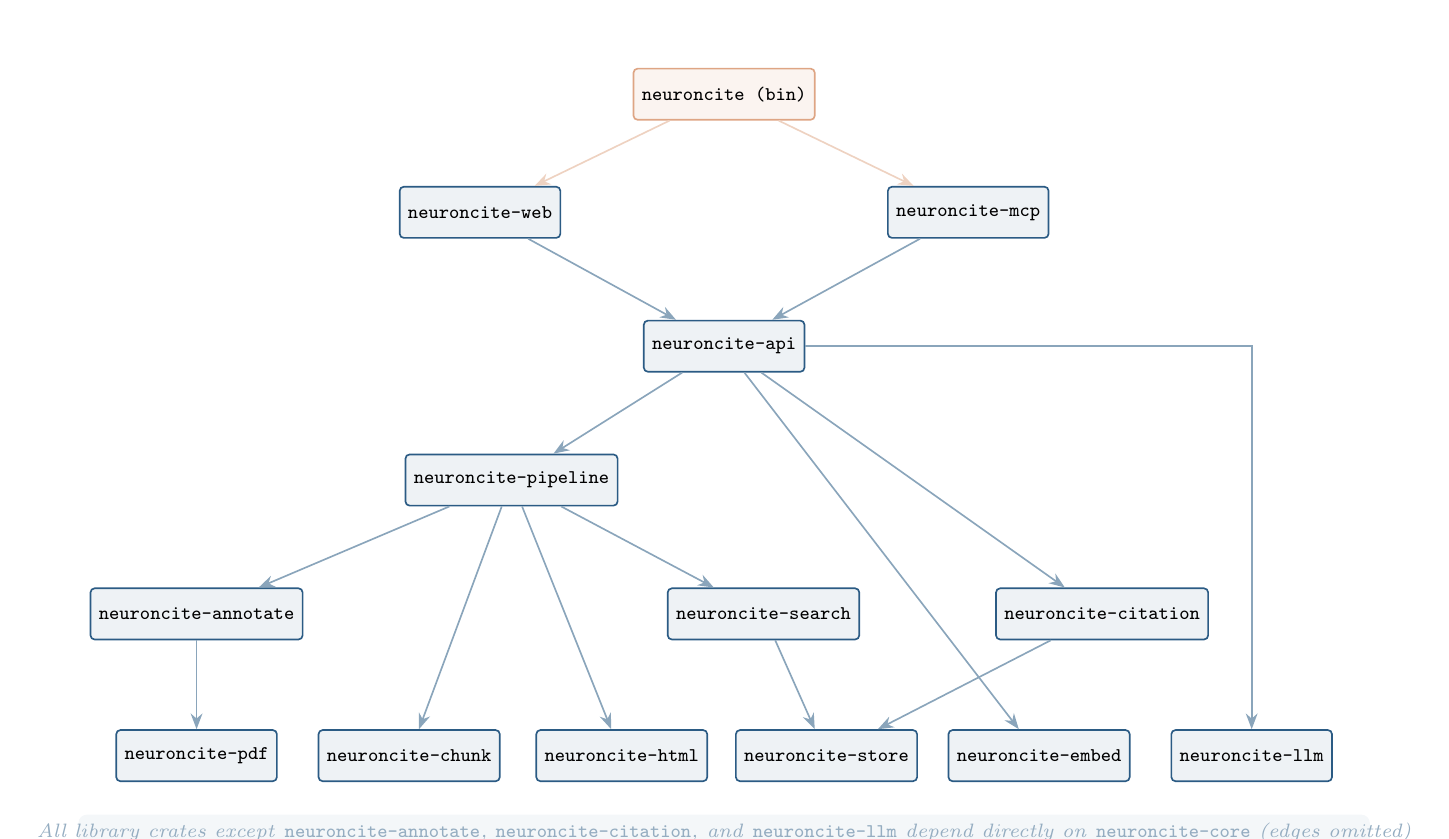
\begin{tikzpicture}[x=1cm, y=1cm,
    % Library crate boxes: rounded rectangles with monospace labels.
    crate/.style={rectangle, draw=cratecolor, fill=cratecolor!8,
                  semithick, rounded corners=1.5pt,
                  minimum height=0.65cm, inner xsep=3pt, inner ysep=1.5pt,
                  font=\scriptsize\ttfamily},
    % Binary crate: distinct color to separate it from library crates.
    bincrate/.style={crate, fill=rustcolor!12, draw=rustcolor},
    % Dependency arrows: from consumer (above) to dependency (below).
    dep/.style={-{Stealth[length=2mm, width=1.5mm]}, semithick,
                color=cratecolor!55},
    % Binary dependency arrows: distinct color matching the binary crate.
    bindep/.style={dep, color=rustcolor!50}
]

    % === Level 0: Foundation crates ===
    % These crates have no workspace-internal dependencies besides core.
    % neuroncite-llm has zero workspace deps (not even core).
    \node[crate] (pdf)   at (1.3,  0) {neuroncite-pdf};
    \node[crate] (chunk) at (4.0,  0) {neuroncite-chunk};
    \node[crate] (html)  at (6.7,  0) {neuroncite-html};
    \node[crate] (store) at (9.3,  0) {neuroncite-store};
    \node[crate] (embed) at (12.0, 0) {neuroncite-embed};
    \node[crate] (llm)   at (14.7, 0) {neuroncite-llm};

    % === Level 1: Single-dependency crates ===
    % Each depends on exactly one Level-0 crate (plus core).
    \node[crate] (annotate) at (1.3,  1.8) {neuroncite-annotate};
    \node[crate] (search)   at (8.5,  1.8) {neuroncite-search};
    \node[crate] (citation) at (12.8, 1.8) {neuroncite-citation};

    % === Level 2: Pipeline ===
    % Orchestrates extraction, chunking, search, and annotation.
    \node[crate] (pipeline) at (5.3, 3.5) {neuroncite-pipeline};

    % === Level 3: API server ===
    % Central integration point: REST handlers, background jobs, workers.
    \node[crate] (api) at (8.0, 5.2) {neuroncite-api};

    % === Level 4: High-level consumers ===
    % Web frontend and MCP protocol server, both backed by the API crate.
    \node[crate] (web) at (4.9, 6.9) {neuroncite-web};
    \node[crate] (mcp) at (11.1, 6.9) {neuroncite-mcp};

    % === Level 5: Binary entry point ===
    \node[bincrate] (bin) at (8.0, 8.4) {neuroncite (bin)};

    % === Core dependency annotation ===
    % Most library crates depend on neuroncite-core directly (12 of 15).
    % neuroncite-annotate and neuroncite-citation obtain core types
    % transitively; neuroncite-llm has zero workspace dependencies.
    % Drawing these edges would dominate the graph, so a text annotation
    % replaces them.
    \fill[cratecolor!5, rounded corners=3pt] (-0.2, -0.75) rectangle (16.2, -1.2);
    \node[font=\scriptsize\itshape, text=cratecolor!50] at (8.0, -0.975)
        {All library crates except \textnormal{\texttt{neuroncite-annotate}},
         \textnormal{\texttt{neuroncite-citation}}, and
         \textnormal{\texttt{neuroncite-llm}} depend directly on
         \textnormal{\texttt{neuroncite-core}} (edges omitted)};

    % === Transitive reduction edges ===
    %
    % The diagram shows the transitive reduction of the full dependency
    % graph: if crate A depends on B and B depends on C, the implied
    % edge A -> C is omitted. This reduces 45+ edges to 15 without
    % losing structural information.

    % Level 0 -> Level 1
    \draw[dep] (annotate) -- (pdf);
    \draw[dep] (search)   -- (store);
    \draw[dep] (citation) -- (store);

    % Level 0/1 -> Level 2 (pipeline)
    \draw[dep] (pipeline) -- (annotate);
    \draw[dep] (pipeline) -- (chunk);
    \draw[dep] (pipeline) -- (html);
    \draw[dep] (pipeline) -- (search);

    % Level 0/1/2 -> Level 3 (api)
    % api reaches store, chunk, pdf, html, search, annotate transitively
    % through pipeline. The four edges below are the non-redundant ones.
    \draw[dep] (api) -- (pipeline);
    \draw[dep] (api) -- (embed);
    \draw[dep] (api) -- (citation);
    % Orthogonal routing: exits api on the right side, runs horizontally
    % to llm's x-coordinate, then drops vertically into llm from the top.
    \draw[dep] (api.east) -| (llm.north);

    % Level 3 -> Level 4 (web, mcp)
    % web reaches pdf, embed, store, llm transitively through api.
    % mcp reaches store, search, embed, annotate, citation, chunk, html
    % transitively through api.
    \draw[dep] (web) -- (api);
    \draw[dep] (mcp) -- (api);

    % Level 4 -> Level 5 (binary)
    % The binary reaches all workspace crates transitively through
    % web and mcp.
    \draw[bindep] (bin) -- (web);
    \draw[bindep] (bin) -- (mcp);

\end{tikzpicture}
\caption{Crate dependency graph (transitive reduction). Arrows point from the consuming
         crate to its dependency. To reduce visual clutter, only non-redundant edges are
         shown: if crate A depends on B and B depends on C, the implied edge A $\to$ C
         is omitted. Most library crates depend directly on \texttt{neuroncite-core}
         for shared domain types; \texttt{neuroncite-annotate} and
         \texttt{neuroncite-citation} obtain core types transitively through
         \texttt{neuroncite-pdf} and \texttt{neuroncite-store} respectively, and
         \texttt{neuroncite-llm} has zero workspace-internal dependencies. These
         edges are replaced by the annotation band at the bottom. The full set of
         direct Cargo.toml dependencies per crate is documented in the crate overview
         table above.}
\label{fig:dep-graph}
\end{figure}

\newpage

\subsection{Internal Module Structure}
\label{sec:module-structure}

The following tables define the internal file and module layout for each library crate.
Every crate follows a shared structural convention: \texttt{src/lib.rs} serves as the
module root that declares submodules and re-exports the crate's public API. It contains
primarily module declarations and re-exports; non-trivial logic is placed in submodules.
Private modules (declared as \texttt{mod}, not \texttt{pub mod}) are not addressable by
downstream crates; only items that are re-exported or otherwise exposed through public
signatures form the crate's public API. The sole exception is \texttt{neuroncite-core},
where all modules are \texttt{pub mod} because it serves as the shared type vocabulary
imported by every other crate.

% --- neuroncite-core ---

\begin{longtable}{>{\ttfamily\small\raggedright\arraybackslash}p{5.2cm}
                   >{\raggedright\arraybackslash}p{2.3cm}
                   >{\raggedright\arraybackslash}p{7cm}}
    \toprule
    \normalfont\textbf{Module Path} & \textbf{Visibility} & \textbf{Responsibility} \\
    \midrule
    \endfirsthead
    \toprule
    \normalfont\textbf{Module Path} & \textbf{Visibility} & \textbf{Responsibility} \\
    \midrule
    \endhead
    \bottomrule
    \endfoot
    src/lib.rs      & public & Declares submodules and re-exports all public types,
                      traits, configuration structs, and error variants. \\
    src/types.rs    & public & Defines the domain value types: \texttt{PageText},
                      \texttt{Chunk}, \texttt{EmbeddedChunk}, \texttt{Citation},
                      \texttt{SearchResult}, \texttt{IndexConfig},
                      \texttt{IndexProgress}, \texttt{ModelInfo},
                      \texttt{ModelManifest}, \texttt{PoolingStrategy}, and
                      \texttt{EmbeddingModelConfig}. \\
    src/traits.rs   & public & Declares the \texttt{EmbeddingBackend},
                      \texttt{ChunkStrategy}, and \texttt{Reranker} trait contracts
                      that downstream crates implement or consume. \\
    src/config.rs   & public & Contains application-wide and session-level
                      configuration structs deserialized from TOML files and CLI
                      arguments. \\
    src/offset.rs   & public & Provides the shared document-offset-to-page resolution
                      algorithm. Accepts a slice of per-page byte counts and a
                      document-level UTF-8 byte offset, and returns the
                      corresponding page number and page-local byte offset. This
                      module is consumed by both \texttt{neuroncite-chunk} (for
                      computing \texttt{page\_start}/\texttt{page\_end} during
                      chunking) and \texttt{neuroncite-search} (for citation
                      generation), avoiding duplication of the offset mapping
                      logic. \\
    src/math.rs     & public & Canonical mathematical utility functions shared across
                      all crates. Provides \texttt{cosine\_similarity(a, b)} which
                      computes the cosine similarity between two \texttt{f32} slices
                      using \texttt{f64} accumulation for numerical stability. Returns
                      0.0 for zero-magnitude vectors. Used by
                      \texttt{neuroncite-search} (reranking) and
                      \texttt{neuroncite-api} (verification). 7 unit tests. \\
    src/paths.rs    & public & Centralized storage path resolution for the
                      application. Computes the base directory
                      (\texttt{Documents/NeuronCite}), runtime directory for
                      driver DLLs (ORT, pdfium, Tesseract), model cache
                      directory for ONNX embedding files, and per-indexed-path
                      database directories under \texttt{indexes/}. Provides
                      \texttt{sanitize\_path} to convert filesystem paths into
                      safe directory names and \texttt{canonicalize\_directory}
                      to resolve a directory to its absolute canonical form
                      (stripping the \texttt{\textbackslash\textbackslash?\textbackslash}
                      UNC prefix on Windows). The canonical path is the single
                      source of truth for all session creation, search, and
                      deletion operations, preventing duplicate sessions when
                      MCP clients pass temporary or non-canonical paths. \\
    src/disk.rs     & public & Cross-platform disk space detection utility.
                      Provides \texttt{available\_disk\_space} (bytes free on the
                      volume containing a given path) and \texttt{check\_disk\_space}
                      (pre-flight check that errors below 500\,MB, warns below
                      1\,GB, and passes otherwise). Uses PowerShell
                      \texttt{Get-PSDrive} on Windows and \texttt{df} on
                      Unix. Consumed by \texttt{neuroncite-pdf} and
                      \texttt{neuroncite-embed} before large runtime downloads. \\
    src/error.rs    & public & Defines the \texttt{NeuronCiteError} enum with
                      \texttt{thiserror}-derived variants covering all failure
                      categories across the application. \\
    src/time.rs     & public & Centralized UNIX timestamp helper. Provides
                      \texttt{unix\_timestamp\_secs() -> i64} that returns the
                      current system time as seconds since the UNIX epoch,
                      falling back to zero if the system clock is before the
                      epoch. Replaces duplicated \texttt{SystemTime} boilerplate
                      across the store and citation crates. \\
    \caption{Internal module structure of \texttt{neuroncite-core}. All modules are
             \texttt{pub mod} because this crate is the shared type vocabulary.}
\end{longtable}

% --- neuroncite-pdf ---

\begin{longtable}{>{\ttfamily\small\raggedright\arraybackslash}p{5.2cm}
                   >{\raggedright\arraybackslash}p{2.3cm}
                   >{\raggedright\arraybackslash}p{7cm}}
    \toprule
    \normalfont\textbf{Module Path} & \textbf{Visibility} & \textbf{Responsibility} \\
    \midrule
    \endfirsthead
    \toprule
    \normalfont\textbf{Module Path} & \textbf{Visibility} & \textbf{Responsibility} \\
    \midrule
    \endhead
    \bottomrule
    \endfoot
    src/lib.rs      & public & Declares submodules and re-exports the file discovery
                      function, page extraction entry point, and
                      \texttt{PdfError}. \\
    src/discovery.rs & private  & Recursively traverses a directory tree, collects PDF
                      file paths with cycle detection via visited-path sets, and
                      returns them in deterministic sorted order. \\
    src/extract/mod.rs & private & Dispatches page extraction to the configured backend
                      and implements the automatic fallback chain (pdf-extract
                      $\to$ pdfium $\to$ OCR). \\
    src/extract/\allowbreak pdf\_extract.rs & public & Wraps the \texttt{pdf-extract}
                      crate to parse PDF content streams and reconstruct text
                      layout on a per-page basis. \\
    src/extract/\allowbreak pdfium.rs & public & Wraps the \texttt{pdfium-render} crate
                      for extraction from PDFs with multi-column layouts, complex
                      tables, and non-standard font encodings. \\
    src/pdfium\_binding.rs & public & Locates the pdfium shared library at runtime
                      by searching the executable directory, the current working
                      directory, the auto-download cache, and system library paths.
                      Falls back to auto-downloading pdfium from GitHub. Used by
                      both the pdfium extraction backend and the OCR module. \\
    src/deps.rs     & public    & Download logic for optional runtime dependencies
                      (pdfium shared library, Tesseract binary, tessdata language
                      packs). Downloads portable distributions and caches them in
                      \texttt{<Documents>/NeuronCite/runtime/}. Uses PowerShell on
                      Windows and curl/tar on Linux/macOS. Public so the web
                      frontend's dependency doctor page can call the download
                      and probe functions. \\
    src/ocr.rs      & public    & Renders pages to raster images at adaptive DPI via
                      pdfium, writes them to temporary files, and invokes the
                      Tesseract CLI binary as a subprocess. Tesseract must be
                      installed via the system package manager or the Doctor
                      panel's install button. \\
    src/quality.rs  & public    & Evaluates extracted text against quality heuristics
                      (alphabetic ratio, replacement character density, line break
                      density, unique token ratio) to decide backend fallback. \\
    src/error.rs    & private   & Defines \texttt{PdfError} with variants for I/O
                      failures, backend extraction failures, OCR failures,
                      dependency download failures, and missing runtime
                      dependencies. \\
    \caption{Internal module structure of \texttt{neuroncite-pdf}.}
\end{longtable}

% --- neuroncite-chunk ---

\begin{longtable}{>{\ttfamily\small\raggedright\arraybackslash}p{5.2cm}
                   >{\raggedright\arraybackslash}p{2.3cm}
                   >{\raggedright\arraybackslash}p{7cm}}
    \toprule
    \normalfont\textbf{Module Path} & \textbf{Visibility} & \textbf{Responsibility} \\
    \midrule
    \endfirsthead
    \toprule
    \normalfont\textbf{Module Path} & \textbf{Visibility} & \textbf{Responsibility} \\
    \midrule
    \endhead
    \bottomrule
    \endfoot
    src/lib.rs      & public & Declares submodules and re-exports a factory function
                      that returns a boxed \texttt{ChunkStrategy} from a strategy
                      identifier string. \\
    src/normalize.rs & public   & Applies deterministic text preprocessing: whitespace
                      collapsing, line-break hyphenation repair, and Unicode NFC
                      normalization. \\
    src/page.rs     & public    & Implements \texttt{ChunkStrategy} for page-based
                      chunking where each PDF page becomes one chunk with its full
                      page text. \\
    src/word\_window.rs & public & Implements \texttt{ChunkStrategy} for sliding
                      word-window chunking with configurable window size and word
                      overlap. \\
    src/token\_window.rs & public & Implements \texttt{ChunkStrategy} for sliding
                      token-window chunking using the model's tokenizer to measure
                      boundaries against the maximum sequence length. The tokenizer
                      instance (from the \texttt{tokenizers} crate) is injected
                      into the strategy constructor by the caller (the API handler
                      or binary crate), which obtains it from the embedding
                      backend. This avoids a compile-time dependency from
                      \texttt{neuroncite-chunk} to \texttt{neuroncite-embed}. \\
    src/sentence.rs & public    & Implements \texttt{ChunkStrategy} for sentence-based
                      chunking using \texttt{unicode-segmentation} with
                      abbreviation-aware boundary suppression. \\
    src/abbreviations.rs & public & Contains the static abbreviation whitelist
                      (\textit{et~al.}, \textit{Fig.}, \textit{Eq.}, etc.)
                      consumed by the sentence chunker to suppress false
                      breaks. \\
    src/offset.rs   & public    & Tracks document-level UTF-8 byte offsets during
                      chunking. Delegates the byte-offset-to-page-number mapping
                      to \texttt{neuroncite\_core::offset} and adds chunk-specific
                      bookkeeping (accumulating offsets across pages, computing
                      \texttt{page\_start}/\texttt{page\_end} for each chunk). \\
    src/error.rs    & public    & Defines \texttt{ChunkError} with variants for
                      normalization failures, invalid parameter combinations, and
                      tokenizer initialization errors. \\
    src/property\_tests.rs & private & Proptest-based property tests covering the
                      \texttt{Page}, \texttt{WordWindow}, and \texttt{Sentence}
                      chunking strategies and normalization invariants. Contains
                      20 tests. Compiled only under \texttt{\#[cfg(test)]}. \\
    \caption{Internal module structure of \texttt{neuroncite-chunk}.}
\end{longtable}

% --- neuroncite-embed ---

\begin{longtable}{>{\ttfamily\small\raggedright\arraybackslash}p{5.2cm}
                   >{\raggedright\arraybackslash}p{2.3cm}
                   >{\raggedright\arraybackslash}p{7cm}}
    \toprule
    \normalfont\textbf{Module Path} & \textbf{Visibility} & \textbf{Responsibility} \\
    \midrule
    \endfirsthead
    \toprule
    \normalfont\textbf{Module Path} & \textbf{Visibility} & \textbf{Responsibility} \\
    \midrule
    \endhead
    \bottomrule
    \endfoot
    src/lib.rs      & public & Conditionally declares backend modules via
                      \texttt{\#[cfg(feature)]} attributes and re-exports the
                      backend registry, shared utilities, and
                      \texttt{EmbedError}. \\
    src/registry.rs & public    & Iterates over all compiled-in backends at runtime,
                      collects their \texttt{ModelInfo} lists, and provides a
                      unified model and backend selection interface. \\
    src/normalize.rs & public   & Normalizes embedding vectors to unit length (L2
                      normalization) so that cosine similarity reduces to a dot
                      product at search time. \\
    src/tokenize.rs & public    & Wraps the HuggingFace \texttt{tokenizers} crate for
                      shared tokenization, padding, and attention mask
                      construction across all backends. \\
    src/cache.rs    & public    & Manages the platform-specific model cache directory
                      (\texttt{\%LOCALAPPDATA\%\textbackslash neuroncite\textbackslash
                      models\textbackslash} on Windows,
                      \texttt{\textasciitilde/.cache/neuroncite/models/} on Linux).
                      Downloads model weights and tokenizer files from Hugging Face
                      Hub on first use, verifies SHA-256 checksums against the
                      \texttt{models.lock} manifest, resolves pinned revisions for
                      reproducible builds, and provides a local file system path to
                      the cached model directory for backend initialization. Supports
                      registration of local model files via \texttt{file://} source
                      URLs. \\
    \midrule
    \multicolumn{3}{l}{\textit{ONNX Runtime backend -- compiled under feature
    \texttt{backend-ort}}} \\
    \midrule
    src/ort/mod.rs  & public    & Backend module root; declares submodules and
                      re-exports \texttt{OrtEmbedder} and
                      \texttt{OrtReranker}. Public to allow downstream
                      crates access to model config functions. \\
    src/ort/embedder.rs & public & Implements \texttt{EmbeddingBackend} for ONNX
                      Runtime with CUDA execution provider selection and batched
                      tensor inference. \\
    src/ort/reranker.rs & public & Implements \texttt{Reranker} for ONNX Runtime
                      cross-encoder models with batched (query, document) pair
                      scoring. \\
    src/ort/session.rs & public & Manages ONNX session lifecycle: execution provider
                      negotiation, GPU memory configuration, and thread pool
                      options. \\
    \midrule
    src/error.rs    & public    & Defines \texttt{EmbedError} with variants for model
                      loading, tokenization, GPU initialization, and inference
                      failures. \\
    \caption{Internal module structure of \texttt{neuroncite-embed}. Backend modules
             are conditionally compiled via Cargo feature flags. The
             \texttt{\#[cfg(feature = "...")]} gate is applied to the
             \texttt{mod} declaration in \texttt{lib.rs}; submodules within each
             backend are implicitly gated.}
\end{longtable}

% --- neuroncite-store ---

\begin{longtable}{>{\ttfamily\small\raggedright\arraybackslash}p{5.2cm}
                   >{\raggedright\arraybackslash}p{2.3cm}
                   >{\raggedright\arraybackslash}p{7cm}}
    \toprule
    \normalfont\textbf{Module Path} & \textbf{Visibility} & \textbf{Responsibility} \\
    \midrule
    \endfirsthead
    \toprule
    \normalfont\textbf{Module Path} & \textbf{Visibility} & \textbf{Responsibility} \\
    \midrule
    \endhead
    \bottomrule
    \endfoot
    src/lib.rs      & public & Declares submodules and re-exports the connection
                      pool builder, repository types, index management functions,
                      workflow types, and \texttt{StoreError}. \\
    src/pool.rs     & private   & Creates and configures the \texttt{r2d2} connection
                      pool with WAL mode, foreign key enforcement, busy timeout,
                      and SQLite PRAGMA tuning. \\
    src/schema.rs   & private   & Contains all DDL statements for tables, indexes,
                      triggers, and the FTS5 virtual table; runs versioned schema
                      migrations on startup. \\
    src/manifest.rs & private   & Reads and writes the \texttt{models.lock} TOML file,
                      recording model revisions, checksums, and tokenizer
                      checksums for index reproducibility. This module is the
                      sole owner of the \texttt{models.lock} file on disk.
                      The \texttt{neuroncite-embed} cache module queries
                      \texttt{neuroncite-store} through a \texttt{ModelManifest}
                      value (defined in \texttt{neuroncite-core}) to verify
                      checksums; it does not access the lock file directly. \\
    src/error.rs    & public    & Defines \texttt{StoreError} with variants for SQLite
                      failures, HNSW serialization errors, manifest parsing
                      errors, and connection pool exhaustion. \\
    \midrule
    \multicolumn{3}{l}{\textit{Repository layer (\texttt{repo/}) -- CRUD operations
    for SQLite tables}} \\
    \midrule
    src/repo/mod.rs & public    & Declares repository submodules and re-exports
                      all repository types for use by downstream crates. \\
    src/repo/session.rs & public & Provides CRUD operations for the
                      \texttt{index\_session} table, including
                      configuration-based session lookup, unique constraint
                      enforcement, \texttt{find\_sessions\_by\_directory} (returns
                      all sessions whose \texttt{directory\_path} matches a given
                      canonical path), and \texttt{delete\_sessions\_by\_directory}
                      (deletes all matching sessions; \texttt{ON DELETE CASCADE}
                      removes child records). \\
    src/repo/file.rs & public   & Provides CRUD operations for the
                      \texttt{indexed\_file} table with two-stage change
                      detection (mtime/size pre-filter, then SHA-256 hash
                      verification). Provides \texttt{find\_file\_by\_session\_path}
                      to look up an existing file record by session ID and file
                      path, used by the change detection step in the indexing
                      pipeline. \\
    src/repo/page.rs & public   & Provides CRUD operations for the \texttt{page}
                      table, including bulk insert of normalized page text and
                      per-page \texttt{byte\_count} computation. \\
    src/repo/chunk.rs & public & Provides CRUD operations for the \texttt{chunk}
                      table, including transactional bulk insert with embedding
                      blobs and batch deletion by file ID. \\
    src/repo/\allowbreak aggregate.rs & public & Reusable SQL aggregate query functions
                      shared by statistics and discovery endpoints. Provides
                      \texttt{all\_session\_aggregates} (per-session file, page,
                      chunk, byte counts), \texttt{file\_chunk\_stats\_by\_session},
                      \texttt{file\_page\_stats\_by\_session},
                      \texttt{browse\_chunks} (paginated chunk browsing),
                      \texttt{find\_files\_by\_path\_pattern} (cross-session file search),
                      and \texttt{session\_quality\_data} (extraction quality per file). \\
    src/repo/\allowbreak annotation\_status.rs & public & Repository functions for the
                      \texttt{annotation\_quote\_status} table. Tracks per-quote
                      progress during annotation pipeline execution. Functions:
                      \texttt{insert\_pending\_quotes} (bulk insert at job start),
                      \texttt{update\_quote\_status} (per-quote update),
                      \texttt{list\_quote\_statuses} (paginated query),
                      \texttt{count\_quote\_statuses\_by\_status} (aggregate
                      counts). \\
    src/repo/diff.rs & public & Session comparison functions. Contains
                      \texttt{FileDiff} and \texttt{SessionDiff} types. The
                      \texttt{diff\_sessions} function compares two sessions by
                      \texttt{file\_path}, classifying files into
                      \texttt{only\_in\_a}, \texttt{only\_in\_b},
                      \texttt{identical}, and \texttt{changed} categories using
                      SHA-256 hash, page count, and file size. \\
    src/repo/\allowbreak web\_source.rs & public & CRUD operations for the
                      \texttt{web\_source} table that stores HTML-specific
                      metadata linked 1:1 to \texttt{indexed\_file} rows.
                      Provides \texttt{insert\_web\_source},
                      \texttt{get\_web\_source\_by\_file},
                      \texttt{get\_web\_source\_by\_url},
                      \texttt{list\_web\_sources} (by session),
                      \texttt{list\_web\_sources\_all}, and
                      \texttt{delete\_web\_source}. \\
    \midrule
    \multicolumn{3}{l}{\textit{Index layer (\texttt{index/}) -- search index
    construction and access}} \\
    \midrule
    src/index/mod.rs & private  & Declares index submodules and re-exports the HNSW
                      management functions, FTS5 operations, and external
                      embedding storage interface. \\
    src/index/hnsw.rs & public & Builds, serializes, deserializes, and rebuilds the
                      HNSW index; tracks orphan counts. The built index is
                      inserted into the per-session \texttt{ArcSwap} map in
                      \texttt{AppState} via \texttt{insert\_hnsw()}. \\
    src/index/fts.rs & public   & Manages the FTS5 virtual table
                      \texttt{chunk\_fts}: four synchronization triggers (INSERT,
                      DELETE, soft-delete, un-delete of \texttt{is\_deleted}),
                      and the optimize maintenance command. \\
    src/index/\allowbreak external.rs & public & Manages the memory-mapped external
                      embeddings file via \texttt{memmap2} for session-scoped
                      embedding storage in large collections. \\
    \midrule
    \multicolumn{3}{l}{\textit{Workflow layer (\texttt{workflow/}) -- job tracking
    and idempotency}} \\
    \midrule
    src/workflow/\allowbreak mod.rs & private & Declares workflow submodules and re-exports
                      job and idempotency repository types. \\
    src/workflow/\allowbreak job.rs & public & Provides CRUD operations for the
                      \texttt{job} table: state transitions, progress updates,
                      and 24-hour retention cleanup. \\
    src/workflow/\allowbreak idempotency.rs & public & Provides CRUD operations for the
                      \texttt{idempotency} table: key lookup, response storage,
                      and expiration cleanup aligned with the job retention
                      window. \\
    \caption{Internal module structure of \texttt{neuroncite-store}. Modules are
             organized into three internal layers: \texttt{repo/} for SQLite table
             CRUD operations, \texttt{index/} for search index file management
             (HNSW, FTS5, external embeddings), and \texttt{workflow/} for
             background job tracking and idempotency. All three layers share the
             same \texttt{r2d2} connection pool configured in \texttt{pool.rs}.}
\end{longtable}

% --- neuroncite-search ---

\begin{longtable}{>{\ttfamily\small\raggedright\arraybackslash}p{5.2cm}
                   >{\raggedright\arraybackslash}p{2.3cm}
                   >{\raggedright\arraybackslash}p{7cm}}
    \toprule
    \normalfont\textbf{Module Path} & \textbf{Visibility} & \textbf{Responsibility} \\
    \midrule
    \endfirsthead
    \toprule
    \normalfont\textbf{Module Path} & \textbf{Visibility} & \textbf{Responsibility} \\
    \midrule
    \endhead
    \bottomrule
    \endfoot
    src/lib.rs      & public & Declares submodules and re-exports the
                      \texttt{SearchPipeline} entry point, search configuration
                      options, \texttt{SearchError}, and refinement functions
                      (\texttt{generate\_sub\_chunks}, \texttt{apply\_refinement},
                      \texttt{parse\_divisors}). \\
    src/pipeline.rs & private   & Orchestrates the full search pipeline: receives
                      the pre-computed query vector, runs parallel retrieval
                      (HNSW + FTS5), fusion, deduplication, reranking, and
                      citation assembly. \\
    src/vector.rs   & private   & Executes HNSW approximate nearest neighbor queries
                      with configurable \texttt{ef\_search} and filters orphaned
                      vector labels against the \texttt{chunk} table. \\
    src/keyword.rs  & private   & Executes FTS5 BM25 keyword queries, converts the
                      raw BM25 scores to 1-indexed rank positions, and returns
                      ranked chunk IDs. \\
    src/fusion.rs   & private   & Merges vector and keyword result lists using
                      Reciprocal Rank Fusion with configurable $k$ parameter and
                      optional BM25 must-match filtering. \\
    src/dedup.rs    & private   & Removes exact-duplicate results by
                      \texttt{content\_hash} and near-duplicate results by
                      SimHash Hamming distance comparison. \\
    src/citation.rs & private   & Generates \texttt{Citation} objects from chunk
                      metadata. Delegates document-level UTF-8 byte offset
                      resolution to \texttt{neuroncite\_core::offset} and
                      assembles the formatted citation string from the resolved
                      page numbers and text excerpts. \\
    src/refine.rs   & public    & Sub-chunk refinement post-processing. Splits each
                      search result chunk into token-based sub-windows at
                      multiple scales (controlled by divisor values), embeds
                      the sub-chunks, and replaces the chunk content with the
                      highest-scoring sub-section when it exceeds the original
                      cosine similarity. Exports \texttt{RefinementConfig},
                      \texttt{generate\_sub\_chunks}, \texttt{apply\_refinement},
                      and \texttt{parse\_divisors}. \\
    src/error.rs    & private   & Defines \texttt{SearchError} with variants for query
                      embedding failures, HNSW query errors, FTS5 query errors,
                      chunk metadata lookup failures, and refinement errors. \\
    \caption{Internal module structure of \texttt{neuroncite-search}.}
\end{longtable}

% --- neuroncite-api ---

\begin{longtable}{>{\ttfamily\small\raggedright\arraybackslash}p{5.2cm}
                   >{\raggedright\arraybackslash}p{2.3cm}
                   >{\raggedright\arraybackslash}p{7cm}}
    \toprule
    \normalfont\textbf{Module Path} & \textbf{Visibility} & \textbf{Responsibility} \\
    \midrule
    \endfirsthead
    \toprule
    \normalfont\textbf{Module Path} & \textbf{Visibility} & \textbf{Responsibility} \\
    \midrule
    \endhead
    \bottomrule
    \endfoot
    src/lib.rs      & public & Declares submodules and re-exports the server
                      builder function, \texttt{AppState}, DTO types, and
                      \texttt{ApiError}. \\
    src/state.rs    & private   & Defines \texttt{AppState} with three composable
                      sub-structs: \texttt{AuthState} (bearer token hash, rate-limit
                      counters, shutdown nonce), \texttt{IndexState} (HNSW index map,
                      vector dimension, progress tracker), and \texttt{SseChannels}
                      (three \texttt{tokio::sync::broadcast::Sender<String>} fields
                      for progress, citation, and source events, initialized
                      unconditionally in \texttt{SseChannels::new()}). Implements the
                      \texttt{PipelineContext} trait from
                      \texttt{neuroncite-pipeline}. \\
    src/router.rs   & private   & Constructs the axum \texttt{Router} with all
                      \texttt{/api/v1/} route registrations, middleware layers,
                      and the OpenAPI JSON endpoint. \\
    \midrule
    \multicolumn{3}{l}{\textit{Request handlers}} \\
    \midrule
    src/handlers/mod.rs & private & Declares handler submodules for each endpoint
                      group. \\
    src/handlers/\allowbreak health.rs & public & Reports application version, build
                      features, GPU availability, and optional dependency
                      status. \\
    src/handlers/\allowbreak index.rs & public & Validates indexing parameters, checks
                      the idempotency key, enforces concurrent job policy, and
                      orchestrates the indexing pipeline by scheduling CPU-bound
                      work via \texttt{spawn\_blocking} and GPU embedding via
                      the GPU worker channel. \\
    src/handlers/\allowbreak search.rs & public & Delegates search and hybrid search
                      requests to the search pipeline and serializes the ranked
                      results. \\
    src/handlers/\allowbreak verify.rs & public & Computes keyword overlap (Jaccard) and
                      semantic similarity (cosine) to produce a weighted evidence
                      verdict. \\
    src/handlers/\allowbreak jobs.rs & public & Queries job state, lists active and
                      historical jobs within the retention window, and triggers
                      cooperative cancellation. \\
    src/handlers/\allowbreak sessions.rs & public & Lists index session configurations,
                      performs cascading deletion of individual sessions
                      (with HNSW eviction), and provides a
                      \texttt{delete\_sessions\_by\_directory} handler that
                      deletes all sessions for a given canonical directory path
                      (also evicting their HNSW graphs from the in-memory map). \\
    src/handlers/\allowbreak documents.rs & public & Retrieves stored page text from the
                      \texttt{page} table by indexed file ID and page
                      number. \\
    src/handlers/\allowbreak backends.rs & public & Returns the list of compiled-in
                      embedding backends with their available models, reranker
                      models, and runtime capabilities (e.g., GPU support). \\
    src/handlers/\allowbreak shutdown.rs & public & Triggers the global
                      \texttt{CancellationToken} for graceful shutdown and
                      returns 202 Accepted (headless mode only). \\
    src/handlers/\allowbreak annotate.rs & public & Handles \texttt{POST /api/v1/annotate}:
                      validates input data (CSV or JSON), creates an annotate
                      job with serialized parameters in \texttt{params\_json},
                      and returns the job ID for progress tracking. \\
    src/handlers/\allowbreak citation.rs & public & Six citation verification handlers:
                      \texttt{create} (parses LaTeX/BibTeX, matches PDFs,
                      assigns batches, inserts citation rows),
                      \texttt{claim} (atomic batch claiming with stale reclaim),
                      \texttt{submit} (accepts verification results, auto-completes
                      job), \texttt{status} (aggregates counts, verdicts, alerts),
                      \texttt{export} (generates annotation CSV, corrections
                      JSON, summary report, triggers annotation pipeline),
                      and \texttt{auto\_verify} (starts a background citation
                      agent that uses a local LLM via the \texttt{LlmBackend}
                      trait to verify all pending rows autonomously). \\
    src/handlers/\allowbreak chunks.rs & public & Handles
                      \texttt{GET /api/v1/sessions/\{id\}/files/\{fid\}/chunks}:
                      paginated chunk browsing for a file with optional page-number
                      filtering. \\
    src/handlers/\allowbreak quality.rs & public & Handles
                      \texttt{GET /api/v1/sessions/\{id\}/quality}:
                      extraction quality report with per-file flags and
                      extraction method distribution summary. \\
    src/handlers/\allowbreak compare.rs & public & Handles
                      \texttt{POST /api/v1/files/compare}:
                      cross-session file comparison by path or name pattern. \\
    src/handlers/\allowbreak discover.rs & public & Handles
                      \texttt{POST /api/v1/discover}:
                      directory-level overview with filesystem scan, session listing,
                      and unindexed PDF detection. \\
    \midrule
    \multicolumn{3}{l}{\textit{Middleware}} \\
    \midrule
    src/middleware/\allowbreak mod.rs & public & Declares middleware submodules for
                      authentication, CORS, and security headers. \\
    src/middleware/\allowbreak auth.rs & public & Extracts and validates the Bearer token
                      from the Authorization header; bypassed when the server is
                      bound to localhost. \\
    src/middleware/\allowbreak cors.rs & public & Configures CORS response headers:
                      omitted for localhost binding, wildcard or explicit origin
                      list for LAN binding. \\
    src/middleware/\allowbreak security\_headers.rs & public & Tower middleware layer that
                      appends defensive response headers
                      (\texttt{X-Content-Type-Options}, \texttt{X-Frame-Options},
                      \texttt{Content-Security-Policy}) to every response. \\
    src/middleware/\allowbreak api\_version.rs & public & Tower middleware layer that appends
                      \texttt{X-API-Version: v1} to every response. Registered in
                      \texttt{router.rs} alongside \texttt{SecurityHeadersLayer} so
                      that every endpoint advertises the active API version without
                      per-handler boilerplate. \\
    \midrule
    \multicolumn{3}{l}{\textit{Service Layer}} \\
    \midrule
    src/service/\allowbreak mod.rs & public & Module declaration for the service layer,
                      which holds business logic shared between REST handlers and MCP
                      handlers. Centralising shared logic here prevents duplication
                      across the two handler trees. \\
    src/service/\allowbreak index.rs & public & Provides the shared
                      \texttt{resolve\_vector\_dimension} function used by both the
                      REST index handler and the MCP index handler. Returns the vector
                      dimension for a given model identifier by querying the model
                      catalog, eliminating the previous duplication between the two
                      handler trees. \\
    \midrule
    \multicolumn{3}{l}{\textit{Indexing Pipeline}} \\
    \midrule
    src/indexer/mod.rs & public & Thin shim re-exporting the complete public API
                      from \texttt{neuroncite-pipeline::indexer}. Sub-module shims
                      (\texttt{batch}, \texttt{pipeline}, \texttt{stdio}) preserve
                      qualified path resolution for intra-crate callers. \\
    src/indexer/\allowbreak batch.rs & public & Glob re-export shim for
                      \texttt{neuroncite\_pipeline::indexer::batch}. Exposes batch
                      size computation, length-sorted permutation, and byte
                      conversion utilities under the \texttt{crate::indexer::batch}
                      path so that test modules inside neuroncite-api continue to
                      resolve without modification. \\
    src/indexer/\allowbreak pipeline.rs & public & Glob re-export shim for
                      \texttt{neuroncite\_pipeline::indexer::pipeline}. Exposes PDF
                      extraction, chunking, embedding, and database insertion
                      functions under the \texttt{crate::indexer::pipeline} path
                      for intra-crate callers. \\
    src/indexer/\allowbreak stdio.rs & public & Glob re-export shim for
                      \texttt{neuroncite\_pipeline::indexer::stdio}. Exposes stdout
                      suppression utilities and the MCP writer flag under the
                      \texttt{crate::indexer::stdio} path for intra-crate callers. \\
    src/html\_indexer.rs & public & Two-phase indexing pipeline for HTML web pages,
                      mirroring the PDF indexer architecture. Phase~1 reads cached
                      HTML from disk, splits content into heading-based sections
                      via \texttt{neuroncite-html}, applies the configured chunk
                      strategy, and computes a SHA-256 content hash. Phase~2
                      embeds chunk text and stores vectors, page records, and
                      \texttt{web\_source} metadata in the database. Provides
                      \texttt{extract\_and\_chunk\_html} (CPU-bound),
                      \texttt{embed\_and\_store\_html} (synchronous), and
                      \texttt{embed\_and\_store\_html\_async} (via WorkerHandle). \\
    src/executor.rs & public    & Thin wrapper shim that re-exports the background
                      job executor from \texttt{neuroncite-pipeline}. Provides
                      \texttt{spawn\_job\_executor}, \texttt{load\_all\_session\_hnsw},
                      \texttt{ensure\_hnsw\_for\_session}, and
                      \texttt{ensure\_hnsw\_for\_session\_async} with
                      \texttt{Arc<AppState>} signatures, coercing to
                      \texttt{Arc<dyn PipelineContext>} internally. \\
    \midrule
    \multicolumn{3}{l}{\textit{GPU Worker}} \\
    \midrule
    src/worker.rs   & private   & Thin shim re-exporting \texttt{WorkerHandle} and
                      \texttt{spawn\_worker} from
                      \texttt{neuroncite-pipeline::worker}. All intra-crate paths
                      (\texttt{crate::worker::WorkerHandle}) resolve through
                      this shim without modification. \\
    \midrule
    src/dto.rs      & private   & Defines JSON request and response structs with
                      \texttt{serde} serialization and \texttt{utoipa} OpenAPI
                      schema annotations. \\
    src/openapi.rs  & private   & Assembles the \texttt{utoipa} OpenAPI 3.1
                      specification from all annotated handler functions, DTO
                      types, and error schemas. \\
    src/agent.rs    & public    & Autonomous citation verification agent driven by a
                      local LLM via the \texttt{LlmBackend} trait. Claims
                      batches from the citation job, prompts the LLM to
                      generate search queries, executes the search pipeline
                      (embedding + HNSW + FTS5), reads page content, prompts
                      the LLM for a structured verdict (JSON), and submits
                      results back to the database. Emits SSE events for
                      per-row phase transitions, streaming reasoning tokens,
                      and aggregate job progress. Runs as a fire-and-forget
                      \texttt{tokio::spawn} background task started by the
                      \texttt{auto\_verify} handler. \\
    src/error.rs    & private   & Defines \texttt{ApiError} and implements axum
                      \texttt{IntoResponse} to map each variant to the
                      appropriate HTTP status code and JSON error body. \\
    src/util.rs     & private   & Internal path validation utilities.
                      \texttt{validate\_path\_containment} verifies that a
                      user-supplied file path resolves to a location within
                      one of the allowed session root directories, rejecting
                      directory traversal attempts. Used by the annotate and
                      citation handlers. \\
    \midrule
    \multicolumn{3}{l}{\textit{Test Infrastructure}} \\
    \midrule
    src/test\_support.rs & private & Shared test utilities compiled only under
                      \texttt{\#[cfg(test)]}:\ stub embedding backend, stub reranker,
                      vector helpers, AppState constructors with in-memory database,
                      and Axum request dispatching helpers. \\
    \caption{Internal module structure of \texttt{neuroncite-api}.}
\end{longtable}

% --- neuroncite-pipeline ---

\begin{longtable}{>{\ttfamily\small\raggedright\arraybackslash}p{5.2cm}
                   >{\raggedright\arraybackslash}p{2.3cm}
                   >{\raggedright\arraybackslash}p{7cm}}
    \toprule
    \normalfont\textbf{Module Path} & \textbf{Visibility} & \textbf{Responsibility} \\
    \midrule
    \endfirsthead
    \toprule
    \normalfont\textbf{Module Path} & \textbf{Visibility} & \textbf{Responsibility} \\
    \midrule
    \endhead
    \bottomrule
    \endfoot
    src/lib.rs      & public & Declares the four public submodules (\texttt{context},
                      \texttt{executor}, \texttt{indexer}, \texttt{worker}) and
                      re-exports the primary public API items. The \texttt{test\_support}
                      module is declared \texttt{pub(crate)} and compiled only under
                      \texttt{\#[cfg(test)]}. \\
    src/context.rs  & public & Defines the \texttt{PipelineContext} trait with 12
                      methods providing access to the database pool, GPU worker
                      handle, HNSW index map, progress tracker, configuration,
                      and SSE channels. Decouples the pipeline from the concrete
                      \texttt{AppState} type in \texttt{neuroncite-api} and
                      enables independent testing via stub implementations. \\
    src/executor.rs & public & Background job executor: \texttt{spawn\_job\_executor}
                      drives the job queue loop, \texttt{load\_all\_session\_hnsw}
                      rebuilds all HNSW indices from stored embeddings on startup,
                      and \texttt{ensure\_hnsw\_for\_session} loads or rebuilds
                      the HNSW index for a single session on demand. Generic over
                      \texttt{Arc<dyn PipelineContext>}. \\
    src/worker.rs   & public & GPU worker management: \texttt{WorkerHandle} holds
                      priority channels for embedding and reranking requests,
                      and \texttt{spawn\_worker} starts the dedicated worker thread
                      that owns the \texttt{EmbeddingBackend} and processes
                      requests via message passing. \\
    \midrule
    \multicolumn{3}{l}{\textit{Indexing Pipeline}} \\
    \midrule
    src/indexer/mod.rs & public & Re-exports \texttt{ExtractionResult},
                      \texttt{ExtractedFile}, and \texttt{FileIndexResult} and
                      all public items from the \texttt{batch}, \texttt{pipeline},
                      and \texttt{stdio} sub-modules so that callers import from
                      a single path. \\
    src/indexer/\allowbreak batch.rs & public & Adaptive batch size computation
                      (\texttt{compute\_batch\_size}) based on sequence length,
                      length-sorted permutation (\texttt{length\_sorted\_permutation},
                      \texttt{restore\_original\_order}) for throughput, and
                      byte-vector conversion utilities (\texttt{f32\_slice\_to\_bytes},
                      \texttt{bytes\_to\_f32\_vec}). \\
    src/indexer/\allowbreak pipeline.rs & public & Two-phase indexing pipeline:
                      \texttt{extract\_and\_chunk\_file} (Phase~1, CPU-bound,
                      parallelizable via rayon) reads and chunks a PDF;
                      \texttt{embed\_and\_store\_file} (Phase~2, synchronous)
                      and \texttt{embed\_and\_store\_file\_async} (Phase~2,
                      routes via \texttt{WorkerHandle}) embed chunks and persist
                      vectors, page records, and file metadata to SQLite. \\
    src/indexer/\allowbreak stdio.rs & public & Stdout suppression for parallel
                      rayon PDF extraction on Windows: \texttt{suppress\_stdout}
                      redirects the CRT file descriptor for stdout to
                      \texttt{/dev/null} (or \texttt{NUL} on Windows),
                      \texttt{restore\_stdout} undoes the redirect.
                      \texttt{StdoutSuppressionGuard} provides RAII-based
                      suppression. Used to silence noisy third-party PDF crates
                      during background indexing without affecting the MCP
                      stdio transport. \\
    \midrule
    \multicolumn{3}{l}{\textit{Test Infrastructure}} \\
    \midrule
    src/test\_support.rs & private & \texttt{StubBackend} test double that implements
                      \texttt{EmbeddingBackend} with deterministic fixed-dimension
                      embeddings. Used by pipeline unit tests in \texttt{executor.rs}
                      and \texttt{worker.rs} to avoid loading real ONNX models.
                      Compiled only under \texttt{\#[cfg(test)]}. \\
    \caption{Internal module structure of \texttt{neuroncite-pipeline}.}
\end{longtable}

% --- neuroncite-web ---

\begin{longtable}{>{\ttfamily\small\raggedright\arraybackslash}p{5.2cm}
                   >{\raggedright\arraybackslash}p{2.3cm}
                   >{\raggedright\arraybackslash}p{7cm}}
    \toprule
    \normalfont\textbf{Module Path} & \textbf{Visibility} & \textbf{Responsibility} \\
    \midrule
    \endfirsthead
    \toprule
    \normalfont\textbf{Module Path} & \textbf{Visibility} & \textbf{Responsibility} \\
    \midrule
    \endhead
    \bottomrule
    \endfoot
    src/lib.rs      & public & Declares submodules and re-exports
                      \texttt{build\_web\_router}, \texttt{WebState}, and
                      \texttt{open\_browser}. Contains the router assembly
                      that merges the existing API router with web-specific
                      handlers, SSE endpoints, and embedded static assets. \\
    src/assets.rs   & public & Embedded static file serving via \texttt{rust-embed}.
                      The compiled SolidJS frontend from \texttt{frontend/dist/}
                      is baked into the binary at compile time. Serves files
                      with correct MIME types and falls back to
                      \texttt{index.html} for SPA client-side routing. \\
    src/sse.rs      & public & Server-Sent Event endpoints for real-time streaming.
                      Registers six SSE streams: \texttt{/logs} (log messages),
                      \texttt{/progress} (indexing progress),
                      \texttt{/jobs} (job state transitions),
                      \texttt{/models} (model operations),
                      \texttt{/citation} (citation verification events), and
                      \texttt{/sources} (source fetching events). Each stream
                      is backed by a \texttt{tokio::sync::broadcast} channel
                      in \texttt{WebState}. Includes a 15-second keep-alive
                      ping interval. \\
    src/broadcast\_layer.rs & public & Tracing \texttt{Layer} implementation that
                      forwards log events to a \texttt{tokio::sync::broadcast}
                      channel for SSE log streaming to the web frontend. Each
                      log event is formatted as a JSON string with level,
                      target, and message fields. \\
    src/browser.rs  & public & Cross-platform browser launcher that opens the
                      default browser to the server URL after startup via the
                      \texttt{opener} crate. Prints the URL to the console as
                      fallback when the browser cannot be opened. \\
    src/native\_window.rs & public & Native OS window creation via \texttt{tao}
                      (event loop) and \texttt{wry} (WebView). Shows a transparent
                      PNG splash screen (via \texttt{splash.rs}) during startup,
                      then transitions to a platform-native application window
                      (WebView2 on Windows, WebKit on macOS/Linux) pointing at
                      the local Axum server URL. The \texttt{tao} event loop runs
                      on the main thread while the Axum server runs in a background
                      \texttt{tokio} thread. Compiled only when the \texttt{gui}
                      feature is enabled. Falls back to browser launch on failure. \\
    src/splash.rs   & public & Transparent splash screen rendering via platform-native
                      APIs. Embeds a pre-rendered PNG (\texttt{assets/splash.png})
                      via \texttt{include\_bytes!} and renders it onto a \texttt{tao}
                      window using Win32 layered windows (\texttt{UpdateLayeredWindow})
                      on Windows, \texttt{NSImageView} on macOS, and Cairo surfaces
                      on Linux. Compiled only when the \texttt{gui} feature is
                      enabled. Called from \texttt{native\_window.rs} during startup
                      to display a frameless transparent splash while the Axum server
                      initializes. \\
    \midrule
    \multicolumn{3}{l}{\textit{Web-specific REST handlers under \texttt{/api/v1/web/}}} \\
    \midrule
    src/handlers/mod.rs & public & Declares handler submodules and assembles the
                      Axum router for all web-specific endpoints. \\
    src/handlers/\allowbreak browse.rs & public & File system browsing and recursive document
                      discovery. Provides directory listing (\texttt{/browse})
                      with drive enumeration on Windows, native OS directory
                      picker (\texttt{/browse/native}), native file picker
                      (\texttt{/browse/native-file}), and document scanning
                      (\texttt{/scan-documents}) with metadata collection. \\
    src/handlers/\allowbreak models.rs & public & Model catalog endpoint returning embedding
                      and reranker models with cached/active status from the
                      static registry in \texttt{neuroncite-embed}. Includes
                      placeholder endpoints for model download and activation. \\
    src/handlers/\allowbreak doctor.rs & public & Dependency probe handlers that check for
                      pdfium (shared library), tesseract (CLI executable), and
                      poppler/pdftotext (CLI executable). Includes a placeholder
                      install endpoint for pdfium. \\
    src/handlers/\allowbreak model\_doctor.rs & public & Model health diagnostics and repair
                      handlers. \texttt{model\_diagnostics} returns file-level
                      cache state for all models in the static registry.
                      \texttt{repair\_model} purges a broken model cache
                      directory and re-downloads all files from HuggingFace. \\
    src/handlers/\allowbreak config.rs & public & Configuration reading endpoint that serializes
                      the \texttt{AppConfig} from \texttt{neuroncite-core} for
                      browser display. \\
    src/handlers/\allowbreak mcp.rs & public & MCP server registration status check, install,
                      and uninstall handlers. Reads the Claude Desktop
                      configuration file to determine registration status and
                      spawns the \texttt{neuroncite mcp install/uninstall}
                      subprocess for registration changes. \\
    src/handlers/\allowbreak ollama.rs & public & Ollama proxy handlers for the web frontend.
                      Seven endpoints: \texttt{ollama\_status} (connectivity check
                      with version info), \texttt{list\_ollama\_models} (installed
                      model list via \texttt{/api/tags}),
                      \texttt{list\_running\_models} (currently loaded models),
                      \texttt{ollama\_catalog} (available model catalog),
                      \texttt{pull\_model} (download a model),
                      \texttt{delete\_model} (remove a model), and
                      \texttt{show\_model} (model metadata and parameters). \\
    src/handlers/\allowbreak setup.rs & public & First-run setup dialog state handlers.
                      \texttt{get\_setup\_status} checks whether the
                      \texttt{.setup\_complete} marker file exists in the
                      NeuronCite data directory and returns the
                      \texttt{is\_first\_run} flag with the data directory
                      path. \texttt{mark\_setup\_complete} creates the marker
                      file to suppress the welcome dialog on future launches. \\
    src/handlers/\allowbreak update.rs & public & Update check handler.
                      Queries the GitHub Releases API to determine whether a
                      newer version of NeuronCite is available. Returns the
                      current version, latest version, an
                      \texttt{update\_available} flag, and a link to the
                      GitHub release page. Does not download or install
                      updates. \\
    src/middleware.rs & public & Security response header middleware for the
                      web router. Applies \texttt{X-Content-Type-Options:~nosniff},
                      \texttt{X-Frame-Options:~DENY}, and
                      \texttt{Referrer-Policy:~strict-origin-when-cross-origin}
                      to all responses served through the web interface. \\
    \caption{Internal module structure of \texttt{neuroncite-web}.}
\end{longtable}

% --- neuroncite-html ---

\begin{longtable}{>{\ttfamily\small\raggedright\arraybackslash}p{5.2cm}
                   >{\raggedright\arraybackslash}p{2.3cm}
                   >{\raggedright\arraybackslash}p{7cm}}
    \toprule
    \normalfont\textbf{Module Path} & \textbf{Visibility} & \textbf{Responsibility} \\
    \midrule
    \endfirsthead
    \toprule
    \normalfont\textbf{Module Path} & \textbf{Visibility} & \textbf{Responsibility} \\
    \midrule
    \endhead
    \bottomrule
    \endfoot
    src/lib.rs      & public & Declares submodules and re-exports the public API:
                      \texttt{HtmlError}, \texttt{WebMetadata}, \texttt{FetchResult},
                      \texttt{HtmlSection}, \texttt{CrawlConfig}, fetch functions,
                      parse functions, and crawl functions. \\
    src/error.rs    & public & Defines \texttt{HtmlError} with variants for HTTP
                      failures, URL parsing, I/O errors, HTML parsing, crawling,
                      caching, invalid arguments, and regex compilation. \\
    src/types.rs    & public & Domain types: \texttt{WebMetadata} (URL, canonical URL,
                      title, Open Graph tags, author, language, domain, HTTP status,
                      fetch timestamp), \texttt{FetchResult} (URL, raw HTML, metadata,
                      cache path), \texttt{HtmlSection} (section index, heading text,
                      heading level, content, byte offsets), and \texttt{CrawlConfig}
                      (start URL, max depth, domain filter, URL pattern, max pages,
                      request delay, sitemap mode, boilerplate stripping). \\
    src/fetch.rs    & public & HTTP fetching with disk caching and URL normalization.
                      \texttt{build\_http\_client} constructs a \texttt{reqwest::Client}
                      with a 30-second timeout, 10-redirect limit, and NeuronCite
                      User-Agent. \texttt{fetch\_url} downloads a page and writes the
                      raw HTML to a SHA-256-named cache file; when the HTTP response
                      is a redirect, the content is written under both the final URL
                      hash and the original URL hash so that callers passing either URL
                      to \texttt{cache\_path\_for\_url} find the cached file.
                      \texttt{fetch\_urls} fetches multiple URLs sequentially with a
                      configurable delay. \texttt{cache\_path\_for\_url} normalizes the
                      URL via \texttt{normalize\_cache\_url} before SHA-256 hashing,
                      stripping tracking parameters (UTM, fbclid, gclid, msclkid),
                      error parameters (error, code), and fragment identifiers to
                      produce stable cache keys independent of dynamic query strings.
                      \texttt{default\_cache\_dir} returns
                      \texttt{\textasciitilde/.neuroncite/html\_cache/}. \\
    src/parse.rs    & public & HTML text extraction and section splitting.
                      \texttt{extract\_visible\_text} strips all tags and returns
                      visible text preserving paragraph structure.
                      \texttt{extract\_main\_content} applies a readability algorithm
                      that scores DOM nodes by text density and penalizes elements
                      with nav/sidebar/footer/ad class names.
                      \texttt{extract\_metadata} reads \texttt{<title>},
                      \texttt{<meta>}, \texttt{<link rel="canonical">}, and
                      Open Graph tags. \texttt{split\_into\_sections} segments
                      content at H1/H2 heading boundaries, producing
                      \texttt{HtmlSection} values with byte offsets.
                      \texttt{sections\_to\_pages} converts sections into
                      \texttt{PageText} values with 1-based page numbers.
                      \texttt{extract\_links} collects and deduplicates
                      \texttt{<a href>} URLs, resolving relative paths. \\
    src/crawl.rs    & public & BFS website crawling and sitemap parsing.
                      \texttt{crawl} performs breadth-first traversal from a
                      start URL, following links up to \texttt{max\_depth} with
                      same-domain filtering and optional regex URL matching.
                      Respects \texttt{max\_pages} and \texttt{delay\_ms}
                      between requests. \texttt{fetch\_sitemap} downloads and
                      parses \texttt{sitemap.xml} to discover URLs.
                      \texttt{normalize\_url} standardizes URLs for deduplication
                      (lowercase scheme/host, remove fragment, remove trailing
                      slash, sort query parameters). \\
    src/download.rs & public & PDF download and URL classification.
                      \texttt{classify\_url} sends an HTTP HEAD request and inspects
                      the Content-Type header and URL path extension to determine
                      whether a URL serves a PDF or an HTML page (returns
                      \texttt{UrlSourceType::Pdf} or \texttt{Html}).
                      \texttt{download\_pdf} downloads a file via GET, validates the
                      Content-Type and \texttt{\%PDF-} magic bytes, and writes the
                      content to disk. \texttt{sanitize\_filename} replaces
                      filesystem-invalid characters and truncates to 200 characters. \\
    src/ssrf.rs     & public & Server-Side Request Forgery (SSRF) protection module.
                      \texttt{validate\_url\_no\_ssrf} parses a URL and rejects
                      requests targeting internal network addresses: IPv4 loopback
                      (127.0.0.0/8), RFC~1918 private ranges (10.0.0.0/8,
                      172.16.0.0/12, 192.168.0.0/16), link-local (169.254.0.0/16),
                      IPv6 loopback (::1), IPv6 link-local (fe80::/10), and
                      IPv4-mapped IPv6 addresses embedding blocked ranges. Called at
                      the entry point of \texttt{fetch\_url}, \texttt{crawl},
                      \texttt{download\_pdf}, and \texttt{fetch\_sitemap}.
                      44 unit tests covering all blocked ranges, boundary addresses,
                      and IPv4-mapped IPv6 bypass attempts. \\
    src/resolve.rs & public & Multi-source DOI resolution chain for obtaining direct
                      open-access PDF URLs. Queries three free academic APIs in
                      sequence: Unpaywall (requires email, no account),
                      Semantic Scholar, and OpenAlex, with a 10-second timeout
                      per API call. Short-circuits on first success.
                      Falls back to \texttt{https://doi.org/\{doi\}} when all APIs
                      fail. Pure parser functions (\texttt{parse\_unpaywall\_response},
                      \texttt{parse\_semantic\_scholar\_response},
                      \texttt{parse\_openalex\_response}) are testable without
                      network access. 21 unit tests. \\
    \caption{Internal module structure of \texttt{neuroncite-html}. The crate depends
             only on \texttt{neuroncite-core} for shared types and uses
             \texttt{reqwest} for HTTP, \texttt{scraper} (html5ever) for DOM parsing,
             and \texttt{url} for URL manipulation.}
\end{longtable}

% --- neuroncite-mcp ---

\begin{longtable}{>{\ttfamily\small\raggedright\arraybackslash}p{5.2cm}
                   >{\raggedright\arraybackslash}p{2.3cm}
                   >{\raggedright\arraybackslash}p{7cm}}
    \toprule
    \normalfont\textbf{Module Path} & \textbf{Visibility} & \textbf{Responsibility} \\
    \midrule
    \endfirsthead
    \toprule
    \normalfont\textbf{Module Path} & \textbf{Visibility} & \textbf{Responsibility} \\
    \midrule
    \endhead
    \bottomrule
    \endfoot
    src/lib.rs      & public & Declares submodules and gates the crate with
                      \texttt{\#![forbid(unsafe\_code)]} and
                      \texttt{\#![deny(warnings)]}. \\
    src/protocol.rs & public & Defines JSON-RPC 2.0 message types: \texttt{JsonRpcRequest},
                      \texttt{JsonRpcResponse}, \texttt{JsonRpcError}. Provides
                      serialization/deserialization for the wire format. \\
    src/transport.rs & public & Line-based stdin/stdout reader and writer.
                      \texttt{StdioReader} reads complete lines from stdin,
                      \texttt{StdioWriter} serializes responses to stdout. Both
                      operate on synchronous I/O; the server loop drives them
                      sequentially. \\
    src/tools.rs    & public & Static MCP tool definitions. Each \texttt{ToolDefinition}
                      contains the tool name, a human-readable description, and a
                      JSON Schema for the input parameters. The \texttt{all\_tools()}
                      function returns the complete catalog of forty-three tools
                      (core search, indexing, annotation, and citation tools
                      plus HTML web scraping tools). \\
    src/dispatch.rs & public & Routes \texttt{tools/call} requests to handler functions.
                      Maps each tool name string to the corresponding handler in the
                      \texttt{handlers} module. Returns a JSON-RPC error for
                      unrecognized tool names. \\
    src/server.rs   & public & The main server loop. Performs the MCP \texttt{initialize}
                      handshake, responds to \texttt{tools/list} with tool definitions,
                      dispatches \texttt{tools/call} to the dispatch layer, and handles
                      \texttt{notifications/cancelled} and shutdown. \\
    src/registration.rs & public & Install/uninstall/status logic for the MCP server entry
                      in Claude Code's configuration file
                      (\texttt{\textasciitilde/.claude/claude\_mcp\_settings.json}).
                      Reads/writes JSON with the server command and arguments. \\
    \midrule
    \multicolumn{3}{l}{\textit{Tool handlers}} \\
    \midrule
    src/handlers/mod.rs & public & Declares handler submodules. All handlers share the
                      same signature: \texttt{async fn(\&Arc<AppState>,
                      \&serde\_json::Value) -> Result<Value, String>}. \\
    src/handlers/search.rs & public & Handles \texttt{neuroncite\_search}: loads the HNSW
                      index, executes vector/hybrid search, and returns ranked
                      passages with citations and scores. \\
    src/handlers/index.rs & public & Handles \texttt{neuroncite\_index}: creates a session
                      and job, spawns the indexing pipeline (PDF extraction,
                      chunking, embedding), and returns the job ID. \\
    src/handlers/batch\_search.rs & public & Handles \texttt{neuroncite\_batch\_search}:
                      executes multiple search queries in a single call with shared
                      HNSW guard and database connection. \\
    src/handlers/files.rs & public & Handles \texttt{neuroncite\_files}: lists all indexed
                      PDF files in a session with file\_id, path, page count, and
                      size. \\
    src/handlers/sessions.rs & public & Handles \texttt{neuroncite\_sessions} (list all
                      sessions), \texttt{neuroncite\_session\_delete} (cascade
                      delete by session ID or by directory path, with HNSW
                      eviction), and \texttt{neuroncite\_session\_update} (set or
                      clear the session label). \\
    src/handlers/jobs.rs & public & Handles \texttt{neuroncite\_jobs} (list all jobs) and
                      \texttt{neuroncite\_job\_status} (retrieve a single job's
                      state, progress, and timestamps). \\
    src/handlers/export.rs & public & Handles \texttt{neuroncite\_export}: formats the most
                      recent search results as Markdown, BibTeX, or CSL-JSON
                      citation output. \\
    src/handlers/models.rs & public & Handles \texttt{neuroncite\_models}: lists all
                      supported embedding models with their dimensions, pooling
                      strategies, and download cache status. \\
    src/handlers/common.rs & public & Shared utility functions for content handlers:
                      \texttt{truncate\_content} (truncates at a UTF-8 boundary
                      at 100\,KB) and \texttt{content\_part\_to\_json} (builds
                      the JSON response object for a single content part with
                      part number, extraction backend, and optional truncation
                      metadata). Used by both \texttt{content.rs} and
                      \texttt{batch\_content.rs}. \\
    src/handlers/content.rs & public & Handles \texttt{neuroncite\_content}: retrieves the full
                      text content of a specific part from the database for
                      context expansion around search results. A ``part'' is
                      the logical content unit of the source format: a page in
                      PDFs, a heading-based section in HTML. Validates
                      parameters before any DB access. Enriches HTML sources
                      with \texttt{web\_source} metadata. \\
    src/handlers/system.rs & public & Handles \texttt{neuroncite\_doctor} and \texttt{neuroncite\_health}: returns runtime
                      diagnostics including GPU availability, loaded backend,
                      database statistics, and feature flags. \\
    src/handlers/\allowbreak annotate.rs & public & Handles \texttt{neuroncite\_annotate}:
                      validates annotation input (CSV or JSON), creates an
                      annotate job with serialized parameters, and returns
                      the job ID and quote count. \\
    src/handlers/\allowbreak citation.rs & public & Five citation verification tool handlers:
                      \texttt{handle\_create} (parses LaTeX/BibTeX, matches
                      PDFs via Jaro-Winkler, assigns batches, creates job),
                      \texttt{handle\_claim} (atomic batch claiming),
                      \texttt{handle\_submit} (accepts results, auto-completes),
                      \texttt{handle\_status} (counts, verdicts, alerts),
                      and \texttt{handle\_export} (generates output files,
                      triggers annotation). \\
    src/handlers/\allowbreak chunks.rs & public & Handles \texttt{neuroncite\_chunks}:
                      browses chunks of a file with pagination and optional
                      page-number filtering. Returns chunk content, page range,
                      word count, and byte count without requiring a search query. \\
    src/handlers/\allowbreak quality.rs & public & Handles \texttt{neuroncite\_quality\_report}:
                      generates text extraction quality flags per file (incomplete
                      extraction, OCR-heavy, low text density, empty pages).
                      Classifies files by extraction method (native, OCR, mixed). \\
    src/handlers/\allowbreak compare.rs & public & Handles \texttt{neuroncite\_file\_compare}:
                      finds the same PDF across different sessions by path pattern,
                      compares chunk counts, content hashes, and chunking strategies
                      to evaluate configuration differences. \\
    src/handlers/\allowbreak discover.rs & public & Handles \texttt{neuroncite\_discover}:
                      scans a directory for PDFs, queries all sessions for that
                      directory, computes unindexed files and per-session aggregate
                      statistics. \\
    src/handlers/\allowbreak inspect.rs & public & Handles
                      \texttt{neuroncite\_inspect\_annotations}: reads annotation
                      properties from a PDF file via pdfium. Returns type,
                      stroke\_color (\texttt{/C}), fill\_color (\texttt{/IC}),
                      alpha, and bounding rectangle per annotation. \\
    src/handlers/\allowbreak batch\_content.rs & public & Handles
                      \texttt{neuroncite\_batch\_content}: retrieves content parts
                      from multiple files in a single call with partial failure
                      reporting. Enforces limits on batch size (10 requests)
                      and total parts (20). Truncates large content at
                      100\,KB. Enriches HTML sources with \texttt{web\_source}
                      metadata. \\
    src/handlers/\allowbreak compare\_search.rs & public & Handles
                      \texttt{neuroncite\_compare\_search}: runs the same query
                      against two sessions and returns side-by-side results
                      with per-session average vector scores for comparing
                      search quality across different chunking strategies or
                      embedding models. \\
    src/handlers/\allowbreak reindex.rs & public & Handles
                      \texttt{neuroncite\_reindex\_file}: re-indexes a single
                      PDF file within an existing session. Deletes old file
                      record (CASCADE), re-extracts, re-chunks, re-embeds,
                      and rebuilds the HNSW index for the session. \\
    src/handlers/\allowbreak index\_add.rs & public & Handles
                      \texttt{neuroncite\_index\_add}: incrementally adds or
                      updates specific PDF files in an existing session. Uses
                      two-stage change detection (mtime/size + SHA-256) to skip
                      unchanged files. Extracts, chunks, embeds, and rebuilds
                      the HNSW index once at the end. \\
    src/handlers/\allowbreak preview\_chunks.rs & public & Handles
                      \texttt{neuroncite\_preview\_chunks}: stateless chunking
                      preview that extracts pages from a single PDF, applies the
                      requested strategy, and returns the first N chunks without
                      database writes. \\
    src/handlers/\allowbreak multi\_search.rs & public & Handles
                      \texttt{neuroncite\_multi\_search}: searches across 2--10
                      index sessions simultaneously. Embeds the query once, runs
                      the search pipeline per session, and merges results into a
                      single ranked list with session\_id attribution. \\
    src/handlers/\allowbreak reranker.rs & public & Handles
                      \texttt{neuroncite\_reranker\_load}: loads a cross-encoder
                      reranker model at runtime and hot-swaps it into the GPU
                      worker via \texttt{ArcSwap}. Activates the \texttt{rerank}
                      parameter in search tools without server restart. \\
    src/handlers/\allowbreak annotate\_status.rs & public & Handles
                      \texttt{neuroncite\_annotate\_status}: returns per-quote
                      progress for annotation jobs including status
                      (pending/matched/not\_found/error), match method, page
                      number, and PDF filename. Validates the job exists and
                      is an annotate job. Supports pagination (limit/offset).
                      Queries the \texttt{annotation\_quote\_status} table. \\
    src/handlers/\allowbreak remove.rs & public & Handles
                      \texttt{neuroncite\_annotation\_remove}: parses parameters
                      (\texttt{pdf\_path}, \texttt{mode}, \texttt{output\_path},
                      \texttt{colors}, \texttt{pages}, \texttt{dry\_run}).
                      Delegates to
                      \texttt{neuroncite\_annotate::remove\_highlights} via
                      \texttt{spawn\_blocking}. Runs in a blocking task
                      because lopdf performs synchronous file I/O. \\
    src/handlers/\allowbreak session\_diff.rs & public & Handles
                      \texttt{neuroncite\_session\_diff}: compares two index
                      sessions to report file differences. Validates both
                      sessions exist. Returns four categories:
                      \texttt{only\_in\_a}, \texttt{only\_in\_b},
                      \texttt{identical}, \texttt{changed}. Delegates to
                      \texttt{neuroncite\_store::diff\_sessions}. \\
    src/handlers/\allowbreak text\_search.rs & public & Handles
                      \texttt{neuroncite\_text\_search}: performs literal
                      substring search within indexed PDF page text stored
                      in the database. Validates the file exists. Returns
                      matching pages with context. Delegates to
                      \texttt{neuroncite\_store::search\_page\_text}. \\
    \midrule
    \multicolumn{3}{l}{\textit{HTML web scraping and indexing tool handlers}} \\
    \midrule
    src/handlers/\allowbreak html\_fetch.rs & public & Handles
                      \texttt{neuroncite\_html\_fetch}: fetches one or more URLs
                      via HTTP GET, caches raw HTML to disk, extracts metadata
                      (title, author, Open Graph tags). Accepts \texttt{urls}
                      array or single \texttt{url} parameter. \\
    src/handlers/\allowbreak html\_crawl.rs & public & Handles
                      \texttt{neuroncite\_html\_crawl}: crawls a website from a
                      start URL with configurable depth, same-domain filtering,
                      URL pattern matching, and sitemap-based discovery. Returns
                      metadata and cache paths for all fetched pages. \\
    \midrule
    \multicolumn{3}{l}{\textit{Citation source acquisition}} \\
    \midrule
    src/handlers/\allowbreak source\_fetch.rs & public & Handles
                      \texttt{neuroncite\_citation\_fetch\_sources}: parses a
                      BibTeX file, extracts \texttt{url} and \texttt{doi} fields,
                      classifies each URL as PDF or HTML via HEAD request,
                      downloads PDFs to disk, fetches HTML pages via the cache
                      pipeline, and indexes all acquired files into the specified
                      session. Filters out bot-detection and Cloudflare challenge
                      pages via \texttt{check\_blocked\_page} (word count below 50
                      plus title/content pattern match). Operates in four phases:
                      fetch and classify (with blocked page filtering), PDF
                      indexing (extract/chunk/embed via the PDF pipeline), HTML
                      indexing (section splitting/chunk/embed via
                      \texttt{html\_indexer}), rebuild HNSW. \\
    \midrule
    src/handlers/\allowbreak bib\_report.rs & public & Handles
                      \texttt{neuroncite\_bib\_report}: parses a BibTeX file, checks
                      file existence in the output directory, and generates CSV and
                      XLSX report files listing all entries with cite\_key, title,
                      author, year, link type (URL/DOI/none), download status
                      (exists/missing/no\_link), and the existing filename. The XLSX
                      workbook includes a formatted data sheet with status-colored
                      rows, badge column, and a summary sheet with aggregate
                      statistics. \\
    % html\_index, html\_page, html\_batch\_page, html\_list, html\_preview
    % were removed in the MCP tool consolidation. Their functionality is
    % absorbed into index.rs (urls param), content.rs, batch\_content.rs,
    % files.rs (source\_type/domain filter), and preview\_chunks.rs (url param).
    \caption{Internal module structure of \texttt{neuroncite-mcp}.}
\end{longtable}

% --- neuroncite-annotate ---

\begin{longtable}{>{\ttfamily\small\raggedright\arraybackslash}p{5.2cm}
                   >{\raggedright\arraybackslash}p{2.3cm}
                   >{\raggedright\arraybackslash}p{7cm}}
    \toprule
    \normalfont\textbf{Module Path} & \textbf{Visibility} & \textbf{Responsibility} \\
    \midrule
    \endfirsthead
    \toprule
    \normalfont\textbf{Module Path} & \textbf{Visibility} & \textbf{Responsibility} \\
    \midrule
    \endhead
    \bottomrule
    \endfoot
    src/lib.rs      & public & Module root, re-exports \texttt{annotate\_pdfs},
                      \texttt{parse\_input}, \texttt{detect\_format},
                      \texttt{inspect\_pdf}, \texttt{inspect\_pdf\_with\_pdfium},
                      \texttt{AnnotateConfig}, \texttt{AnnotationDetail},
                      \texttt{InspectionResult}, \texttt{InputFormat}, and
                      \texttt{InputRow}. \\
    src/error.rs    & public & \texttt{AnnotateError} enum with variants covering
                      input parsing, PDF discovery, quote location, annotation
                      creation, save, and verification failures. \\
    src/types.rs    & public & Core types: \texttt{AnnotateConfig},
                      \texttt{InputRow}, \texttt{InputFormat},
                      \texttt{Color}, \texttt{MatchMethod},
                      \texttt{MatchResult}, \texttt{PreCheckResult},
                      \texttt{PostCheckResult}. \\
    src/input.rs    & private & CSV and JSON input parsing with automatic format
                      detection. Validates required fields (title, author, quote)
                      and optional fields (color as \texttt{\#RRGGBB} hex,
                      comment text). \\
    src/resolve.rs  & public  & Fuzzy PDF filename matching. Extracts title and
                      author from filenames via regex, computes Jaro-Winkler
                      similarity with weighted scoring ($0.6 \times \text{title} +
                      0.4 \times \text{author}$), and groups input rows by
                      matching PDF file. Threshold: 0.80. Public because the
                      MCP annotate handler calls \texttt{match\_pdfs\_to\_quotes}
                      directly for dry-run validation. \\
    src/locate.rs   & private & 4-stage text location pipeline. Stage~1: exact
                      \texttt{str::find()} on pdfium-extracted page text.
                      Stage~2: normalized match (Unicode NFC, soft-hyphen
                      removal, whitespace collapse). Stage~3: fuzzy match via
                      Levenshtein sliding window ($\geq 90\%$ threshold).
                      Stage~4: OCR fallback via Tesseract hOCR bounding boxes
                      (feature-gated). \\
    src/annotate.rs & private & Creates pdfium highlight and text annotations.
                      Merges per-character bounding boxes into line-level
                      rectangles. Uses \texttt{set\_bounds()},
                      \texttt{set\_stroke\_color()} (writes the \texttt{/C}
                      entry for PDF viewer display), and
                      \texttt{set\_fill\_color()} (writes the \texttt{/IC}
                      entry for compatibility). \\
    src/appearance.rs & public & lopdf-based post-processing that injects
                      \texttt{/AP} (Appearance Stream) entries into highlight
                      annotations. pdfium-render creates highlights with
                      \texttt{/Rect}, \texttt{/QuadPoints}, \texttt{/C},
                      \texttt{/IC} but without \texttt{/AP}. Most PDF viewers
                      require the \texttt{/AP /N} Form XObject to render the
                      colored overlay. Generates compliant Form XObject
                      appearance streams with Multiply blend mode and 50\%
                      opacity. Runs after pdfium save and before post-check
                      verification. \\
    src/inspect.rs  & public & Read-only PDF annotation inspector. Scans all
                      annotations via pdfium and extracts type, stroke\_color
                      (\texttt{/C}), fill\_color (\texttt{/IC}), alpha, and
                      bounding rectangle. Used by the
                      \texttt{neuroncite\_inspect\_annotations} MCP tool for
                      agent-driven color verification after annotation. \\
    src/verify.rs   & public & Pre-check (validates bounding box coverage $\geq
                      95\%$) and post-check (verifies annotation count and
                      area within $\pm 15\%$ tolerance after save). \\
    src/report.rs   & public & \texttt{AnnotationReport}, \texttt{PdfReport},
                      \texttt{QuoteReport}, \texttt{ReportSummary}, and
                      \texttt{UnmatchedInput} structs. JSON-serializable
                      report saved to the output directory. \\
    src/pipeline.rs & private & Pipeline orchestration: resolves PDFs, iterates
                      matched groups, locates quotes, creates annotations,
                      saves results, and generates the final report. \\
    src/remove.rs   & public & Removes highlight annotations from PDFs using
                      lopdf (pure Rust). Supports three removal modes:
                      \texttt{All} (all highlights), \texttt{ByColor}
                      (matching specific hex colors), \texttt{ByPage}
                      (specific page numbers). Two-pass algorithm: pass~1
                      collects annotation targets by filtering on
                      \texttt{/Subtype=Highlight} and mode criteria, pass~2
                      removes matching annotation \texttt{ObjectId}s from page
                      \texttt{/Annots} arrays and deletes orphaned objects.
                      Supports \texttt{dry\_run} mode and separate
                      \texttt{output\_path}. Depends on \texttt{inspect.rs}
                      helpers (\texttt{read\_subtype\_str},
                      \texttt{read\_color\_entry}, etc.) for reading
                      annotation properties. \\
    \caption{Internal module structure of \texttt{neuroncite-annotate}.}
\end{longtable}

% --- neuroncite-citation ---

\begin{longtable}{>{\ttfamily\small\raggedright\arraybackslash}p{5.2cm}
                   >{\raggedright\arraybackslash}p{2.3cm}
                   >{\raggedright\arraybackslash}p{7cm}}
    \toprule
    \normalfont\textbf{Module Path} & \textbf{Visibility} & \textbf{Responsibility} \\
    \midrule
    \endfirsthead
    \toprule
    \normalfont\textbf{Module Path} & \textbf{Visibility} & \textbf{Responsibility} \\
    \midrule
    \endhead
    \bottomrule
    \endfoot
    src/lib.rs      & public & Module root, re-exports all primary types:
                      \texttt{Verdict}, \texttt{CorrectionType},
                      \texttt{CitationRow}, \texttt{CitationRowInsert},
                      \texttt{BatchClaim}, \texttt{SubmitEntry},
                      \texttt{CitationJobParams}, \texttt{Alert},
                      \texttt{ExportSummary}. Declares submodules. \\
    src/error.rs    & public & \texttt{CitationError} enum with variants
                      covering TeX/Bib file reading, unresolved cite-keys,
                      database errors, JSON serialization, CSV generation,
                      and I/O failures. \\
    src/types.rs    & public & Data types for all pipeline stages:
                      \texttt{Verdict} (6 variants with color mapping),
                      \texttt{CorrectionType} (4 variants),
                      \texttt{RawCitation}, \texttt{BibEntry},
                      \texttt{CitationRow} (19-column DB row),
                      \texttt{CitationRowInsert},
                      \texttt{BatchClaim}, \texttt{SubmitEntry},
                      \texttt{PassageRef}, \texttt{LatexCorrection},
                      \texttt{StatusCounts}, \texttt{BatchCounts},
                      \texttt{StatusReport}, \texttt{ExportResult},
                      \texttt{ExportSummary}, \texttt{CitationJobParams}. \\
    src/latex.rs    & public & LaTeX citation parser. Extracts
                      \texttt{\textbackslash cite}, \texttt{\textbackslash citep},
                      \texttt{\textbackslash citet}, \texttt{\textbackslash autocite},
                      \texttt{\textbackslash parencite}, and
                      \texttt{\textbackslash textcite} commands with line numbers,
                      anchor words, section headings, and group IDs for
                      multi-key citations. \\
    src/bibtex.rs   & public & BibTeX parser. Extracts entries by cite-key
                      with author, title, year, abstract, and keywords.
                      Handles brace-delimited and quote-delimited field
                      values with case-insensitive field names. \\
    src/batch.rs    & public & Batch assignment. Groups nearby citations by
                      section proximity into batches of configurable size.
                      Citations sharing a \texttt{group\_id} (from the same
                      \texttt{\textbackslash cite\{a,b,c\}} command) are
                      kept together. \\
    src/db.rs       & public & SQLite CRUD operations for the
                      \texttt{citation\_row} table: insert rows, claim the
                      next pending batch (with 5-minute stale reclaim),
                      submit batch results, count rows and batches by
                      status, aggregate verdicts, and build alert entries
                      from flagged rows. \\
    src/export.rs   & public & Export functions: builds annotation CSV
                      (verdict-colored), corrections JSON sorted by
                      \texttt{tex\_line}, and a summary report JSON with
                      statistics and alert counts. \\
    \caption{Internal module structure of \texttt{neuroncite-citation}.}
\end{longtable}

% --- neuroncite-llm ---

\begin{longtable}{>{\ttfamily\small\raggedright\arraybackslash}p{5.2cm}
                   >{\raggedright\arraybackslash}p{2.3cm}
                   >{\raggedright\arraybackslash}p{7cm}}
    \toprule
    \normalfont\textbf{Module Path} & \textbf{Visibility} & \textbf{Responsibility} \\
    \midrule
    \endfirsthead
    \toprule
    \normalfont\textbf{Module Path} & \textbf{Visibility} & \textbf{Responsibility} \\
    \midrule
    \endhead
    \bottomrule
    \endfoot
    src/lib.rs      & public & Declares submodules and re-exports the
                      \texttt{LlmBackend} trait, type definitions, error
                      types, and the \texttt{OllamaBackend} implementation.
                      Defines the \texttt{LlmBackend} trait with
                      \texttt{chat\_completion} (blocking) and
                      \texttt{chat\_completion\_streaming} (token-by-token
                      callback) methods returning
                      \texttt{Pin<Box<dyn Future>>} for object safety. \\
    src/types.rs    & public & Data structures for LLM communication:
                      \texttt{ChatRole} (System, User, Assistant),
                      \texttt{ChatMessage}, \texttt{LlmResponse} (with
                      optional token counts), and \texttt{LlmConfig}
                      (base URL, model name, temperature, max tokens). \\
    src/error.rs    & public & Error enumeration for LLM operations:
                      \texttt{ConnectionFailed}, \texttt{RequestFailed}
                      (with HTTP status and body), \texttt{ParseError},
                      \texttt{SchemaViolation}, \texttt{ModelNotFound},
                      and \texttt{Timeout}. \\
    src/ollama.rs   & public & Concrete \texttt{LlmBackend} implementation for
                      the Ollama HTTP API. \texttt{chat\_completion} sends
                      POST \texttt{/api/chat} with \texttt{stream:~false}.
                      \texttt{chat\_completion\_streaming} sends POST
                      \texttt{/api/chat} with \texttt{stream:~true} and
                      reads NDJSON line-by-line via
                      \texttt{reqwest::Response::bytes\_stream()}, invoking
                      the \texttt{on\_token} callback per chunk.
                      \texttt{list\_models} queries GET \texttt{/api/tags}
                      for installed model metadata. \\
    \caption{Internal module structure of \texttt{neuroncite-llm}.}
\end{longtable}

\newpage

% ============================================================
% 3. CORE ABSTRACTIONS
% ============================================================
\section{Core Abstractions}

The \texttt{neuroncite-core} crate defines all shared types and trait contracts that the
other crates depend on. It contains primarily data structures, trait signatures,
configuration types, and a unified error enumeration, with no domain-specific processing
logic.

\subsection{Domain Types}

\begin{traitbox}[Domain Types]
\begin{description}[style=nextline, labelwidth=3.5cm, leftmargin=3.8cm]
    \item[\texttt{PageText}]
        Represents the extracted text of a single PDF page. Fields: source file path,
        page number (one-indexed), the raw text content as a string, and the extraction
        backend that produced it (\texttt{pdf\_extract}, \texttt{pdfium}, or
        \texttt{ocr}).

    \item[\texttt{Chunk}]
        A text fragment produced by a chunking strategy. Fields: source file path,
        page number start (one-indexed), page number end (equal to page number start
        for single-page chunks, greater for chunks spanning page boundaries),
        chunk index within the document (zero-indexed, sequential across all pages),
        document text offset start and end (UTF-8 byte positions within the
        concatenated, normalized full-document text), the text content, and a SHA-256
        content hash for deduplication.

    \item[\texttt{EmbeddedChunk}]
        A chunk together with its dense vector embedding. Fields: all fields from
        \texttt{Chunk} plus the embedding as a vector of 32-bit floats.

    \item[\texttt{Citation}]
        A structured reference to the source of a search result. Fields: source file
        path, file display name (without directory prefix), page number start, page
        number end (for chunks spanning page boundaries), document-level UTF-8 byte
        offset start and end (resolved to page-local positions for display), and a
        pre-formatted citation string
        (e.g., ``pagan1996.pdf, p.\,17: \textit{``Financial econometrics has
        emerged...''}'').

    \item[\texttt{SearchResult}]
        A single ranked result returned by a search query. Fields: final ranking score
        (the RRF score from hybrid fusion, or the reranker score if reranking was
        applied -- this is the primary sort key), vector similarity score (diagnostic,
        included for transparency), BM25 rank position (diagnostic, included for
        transparency; SQLite FTS5 \texttt{bm25()} returns a lower-is-better score,
        so this field stores the rank position rather than the raw BM25 value),
        reranker score (if reranking was applied), source file path, page number start,
        page number end, chunk index, the text content, and a \texttt{Citation}
        instance.

    \item[\texttt{IndexConfig}]
        Captures the full configuration of an indexing session. Fields: directory path,
        embedding model name, chunking strategy identifier, chunk size, chunk overlap,
        maximum words per chunk (sentence-based strategy), OCR language string,
        embedding storage mode (sqlite\_blob or mmap\_file), and the vector
        dimensionality. All fields that participate in the session uniqueness constraint
        (see Section~\ref{sec:session-table}) are present in this type.

    \item[\texttt{IndexProgress}]
        Reports the current state of an ongoing indexing operation. Fields: total number
        of files discovered, number of files processed so far, total number of chunks
        created, and a boolean indicating whether the operation is complete.

    \item[\texttt{PoolingStrategy}]
        Enum that determines how the final embedding vector is extracted from a
        transformer model's output tensor. Three variants:
        \texttt{Cls} (extract the [CLS] token at position 0, used by BERT-family models),
        \texttt{MeanPooling} (attention-weighted mean over all non-padding tokens, used by
        Qwen3-Embedding and similar decoder models),
        \texttt{LastToken} (extract the embedding at the last non-padding position,
        reserved for causal decoder models).

    \item[\texttt{EmbeddingModelConfig}]
        Static configuration for a single embedding model. Encapsulates all parameters
        that differ between encoder (BERT, GTE-Large) and decoder (Qwen) architectures:
        model identifier, display name, vector dimension, maximum sequence length (512
        for standard BERT, 8192 for GTE-Large and decoder models), pooling strategy,
        whether the model requires \texttt{token\_type\_ids} input tensor, whether the
        ONNX model requires explicit \texttt{position\_ids} (for rotary position embeddings),
        and optional instruction prefix strings (\texttt{query\_prefix},
        \texttt{document\_prefix}) for decoder models that use instruction-tuned embeddings.

    \item[\texttt{ModelInfo}]
        Describes an available embedding model. Fields: model identifier string, display
        name, vector dimensionality, and the backend that provides it.

    \item[\texttt{ModelManifest}]
        Tracks a downloaded model for reproducibility and offline operation. Fields:
        model identifier string, revision hash (the specific Hugging Face commit),
        SHA-256 checksum of the model weights file, source URL, license identifier
        (e.g., ``MIT'', ``Apache-2.0''), and a local file system path hint pointing
        to the cached model directory (re-resolved on each launch; not a hard
        requirement for portability). A manifest file (\texttt{models.lock}) in the
        \texttt{.neuroncite/} directory records all models used by the current index,
        analogous to \texttt{Cargo.lock} for Rust dependencies.
\end{description}
\end{traitbox}

\subsection{The Embedding Backend Trait}

\begin{traitbox}[EmbeddingBackend Trait]
The central abstraction for all machine-learning backends. The ort backend
provides an implementation of this trait. The trait is object-safe and uses dynamic
dispatch so that the web server and API can hold a reference to the active backend without
knowing its concrete type at compile time.

\textbf{Required methods:}
\begin{description}[style=nextline, labelwidth=4.5cm, leftmargin=4.8cm, noitemsep]
    \item[\texttt{name}]
        Returns the human-readable name of the backend (e.g., ``ONNX Runtime'').
    \item[\texttt{vector\_dimension}]
        Returns the dimensionality of the embedding vectors produced by the currently
        loaded model (e.g., 384 for bge-small-en-v1.5).
    \item[\texttt{load\_model}]
        Loads a specific model by identifier string. This may involve downloading model
        weights on first use and initializing a GPU session.
    \item[\texttt{embed\_batch}]
        Accepts a slice of text strings and returns a vector of embedding vectors. This
        is the primary hot path and must leverage GPU parallelism.
    \item[\texttt{embed\_single}]
        Convenience method that embeds a single text string. Delegates to
        \texttt{embed\_batch} with a one-element slice.
    \item[\texttt{supports\_gpu}]
        Returns whether this backend was compiled with GPU support and whether a
        compatible GPU is currently available.
    \item[\texttt{available\_models}]
        Returns a list of \texttt{ModelInfo} structures describing all models this
        backend can load.
\end{description}
\end{traitbox}

\subsection{The Reranker Trait}

\begin{traitbox}[Reranker Trait]
Abstracts over cross-encoder models that score (query, document) pairs. Unlike the
\texttt{EmbeddingBackend} trait, which produces independent vector representations,
a reranker jointly attends to both query and document text and outputs a single
relevance score. This produces higher-quality relevance judgments than cosine
similarity alone, at the cost of being unable to pre-compute document representations.

\textbf{Required methods:}
\begin{description}[style=nextline, labelwidth=4.5cm, leftmargin=4.8cm, noitemsep]
    \item[\texttt{name}]
        Returns the human-readable name of the reranker model.
    \item[\texttt{rerank\_batch}]
        Accepts a query string and a slice of candidate document texts. Returns a
        vector of relevance scores (one per candidate), where higher scores indicate
        stronger relevance. The reranker processes all pairs on the GPU in a single
        batched forward pass.
    \item[\texttt{load\_model}]
        Loads a cross-encoder model by identifier string.
\end{description}

The embedding backend (ort) provides a corresponding reranker
implementation behind the same feature flag. The reranker is an optional component:
if no reranker model is configured, the search pipeline skips the reranking stage and
returns results ranked by the hybrid score alone.
\end{traitbox}

\subsection{The Chunk Strategy Trait}

\begin{traitbox}[ChunkStrategy Trait]
Abstracts over different text splitting approaches. Each strategy receives a list of
\texttt{PageText} values (the full extracted text of a document, page by page) and
produces a list of \texttt{Chunk} values.

\textbf{Required method:}
\begin{description}[style=nextline, labelwidth=3cm, leftmargin=3.3cm, noitemsep]
    \item[\texttt{chunk}]
        Accepts a slice of \texttt{PageText} and returns a vector of \texttt{Chunk}.
        The implementation determines how text is split and what metadata is attached.
        Each chunk records its UTF-8 byte offset range within the concatenated,
        normalized full-document text, and the page range it spans.
\end{description}

\textbf{Provided strategies:}
\begin{description}[style=nextline, labelwidth=3cm, leftmargin=3.3cm, noitemsep]
    \item[Page-based]
        Each PDF page becomes one chunk. The simplest strategy, suitable for documents
        where page boundaries carry semantic meaning.
    \item[Word-window]
        A sliding window of configurable word count with configurable overlap. Parameters:
        \textit{window\_size} (number of words per chunk) and \textit{overlap} (number of
        words shared between consecutive chunks).
    \item[Token-window]
        A sliding window measured in model tokens rather than whitespace-separated
        words. Uses the tokenizer of the active embedding model to count tokens,
        ensuring that each chunk fits within the model's maximum sequence length.
        Parameters: \textit{token\_limit} and \textit{token\_overlap}. Produces
        deterministic chunk boundaries for a given model and text.
    \item[Sentence-based]
        Splits text at sentence boundaries using the \texttt{unicode-seg\-men\-ta\-tion}
        crate. Groups consecutive sentences until a configurable maximum word count is
        reached. Uses an abbreviation whitelist to avoid false sentence breaks.
\end{description}
\end{traitbox}

\newpage

% ============================================================
% 4. PDF EXTRACTION PIPELINE
% ============================================================
\section{PDF Extraction Pipeline}

The \texttt{neuroncite-pdf} crate is responsible for three tasks: discovering PDF files in a
directory tree, extracting their textual content through multiple backends, and
triggering OCR for pages where text extraction fails.

\subsection{File Discovery}

Given a root directory path, the crate recursively traverses all subdirectories and
collects every file with a \texttt{.pdf} extension (case-insensitive). The traversal
uses Rust's standard library directory iterator and filters by extension. Symbolic links
are followed, with cycle detection via a visited-inode set (on Linux) or
canonicalized-path set (on Windows) to prevent infinite loops caused by circular
symlinks. Unreadable directories are skipped with a warning logged to the progress
channel, but do not abort the overall discovery.

The result is an ordered list of absolute file paths, sorted alphabetically for
deterministic processing order.

\subsection{Extraction Backends}

The crate supports two text extraction backends. The user can configure which backend
to use, or leave the default automatic selection.

\begin{designbox}[Primary Backend: pdf-extract]
The \texttt{pdf-extract} crate parses PDF content streams and reconstructs text layout.
It is fast, pure Rust, and requires no external dependencies. It handles the majority
of well-formed PDF documents correctly. This is the default backend.
\end{designbox}

\begin{designbox}[Fallback Backend: pdfium]
The \texttt{pdfium-render} crate provides Rust bindings to Google's PDFium library
(the rendering engine used in Chromium). PDFium handles complex PDF features that
\texttt{pdf-extract} struggles with: multi-column layouts, tables with cell boundaries,
non-standard font encodings, and PDFs produced by certain commercial tools.

The pdfium backend requires the PDFium shared library to be present at runtime. On
Windows, this is \texttt{pdfium.dll}; on Linux, \texttt{libpdfium.so}. The library is
bundled alongside the executable or downloaded on first use.
\end{designbox}

\textbf{Automatic backend selection:} When set to ``auto'' mode, the system first
attempts extraction with \texttt{pdf-extract}. The extracted text is evaluated against
multiple quality heuristics to decide whether to fall back to pdfium:

\begin{itemize}[noitemsep]
    \item \textbf{Alphabetic ratio:} If the ratio of alphabetic characters to total
          characters falls below a configurable threshold (default 0.3), the text is
          likely garbled due to encoding issues.
    \item \textbf{Replacement character ratio:} If the ratio of Unicode replacement
          characters (\texttt{U+FFFD}) and other common substitution markers to total
          characters exceeds a configurable threshold (default 0.05), the font encoding
          was not decoded correctly.
    \item \textbf{Line break density:} If the number of line break characters per total
          character count exceeds a configurable threshold (default 0.15), the layout
          reconstruction fragmented continuous text into single-character or single-word
          lines.
    \item \textbf{Unique token ratio:} If the ratio of unique whitespace-separated tokens
          to total tokens falls below a configurable threshold (default 0.05), the text
          consists of repetitive garbage output rather than natural language.
\end{itemize}

If any heuristic fails, the page is re-extracted using pdfium. This catches cases where
\texttt{pdf-extract} returns garbled output due to encoding issues, fragmented multi-column
layouts, or non-standard font mappings.

\subsection{Automatic OCR Fallback}

For pages where both text extraction backends produce insufficient text (fewer than 20
non-whitespace characters), the system assumes the page contains scanned or image-based
content and triggers OCR:

\begin{enumerate}[noitemsep]
    \item The page is rendered to a raster image (PNG) at an adaptive DPI setting using
          pdfium's rendering capabilities (see below).
    \item The rendered PNG image is written to a temporary file and passed to the
          Tesseract CLI binary as a subprocess (\texttt{tesseract <file> stdout -l <lang>}).
          Tesseract is located on the system PATH or in the Doctor panel's
          download cache. It must be installed beforehand via the system package
          manager or the Doctor panel's install button (UB-Mannheim installer on
          Windows, AppImage on Linux).
    \item The OCR output replaces the empty extraction result.
    \item The \texttt{PageText} is annotated with extraction backend \texttt{ocr} so that
          downstream components can distinguish OCR text from directly extracted text.
\end{enumerate}

\textbf{Adaptive DPI:} The render resolution for OCR is selected based on the page
dimensions and content density. Pages with physical dimensions smaller than
$150 \times 200$\,mm (approximately A5 or smaller) are rendered at 400 DPI to capture
fine detail. All other pages use the default of 300 DPI. The user can override this
behavior by setting a fixed DPI value in the session configuration.

\textbf{OCR language configuration:} Tesseract requires trained language data files
(tessdata) for each language it recognizes. The OCR language is configurable per session
through the web frontend settings or the API \texttt{/api/v1/index} request field
\texttt{ocr\_language} (default: \texttt{eng}). Multiple languages can be specified as
a \texttt{+}-separated string (e.g., \texttt{eng+deu} for English and German). The web
frontend provides a dropdown populated with all \texttt{.traineddata} files found in
the Tesseract data directory.

\begin{notebox}[OCR Dependency]
OCR requires the Tesseract engine and trained language data files to be installed on
the system. If Tesseract is not available, the OCR step is skipped and the page is
included with empty text. The web frontend displays a warning listing pages that could
not be processed and the reason (missing Tesseract binary or missing language data).
\end{notebox}

\subsection{Text Extraction Output}

Each page produces one \texttt{PageText} value containing:
\begin{itemize}[noitemsep]
    \item The absolute path to the source PDF file
    \item The one-indexed page number
    \item The extracted text as a UTF-8 string
    \item The extraction backend identifier (\texttt{pdf\_extract}, \texttt{pdfium}, or \texttt{ocr})
\end{itemize}

Pages that yield empty text after all backend attempts are included in the output with
an empty string. This preserves correct page numbering for subsequent chunking and result
display.

\subsection{Error Handling}

If a PDF file cannot be opened (corrupted, password-protected, or unsupported format),
the error is recorded and the file is skipped. Processing continues with the remaining
files. The final extraction summary reports the count of successfully processed files
and the count of skipped files with their error reasons.

\newpage

% ============================================================
% 4b. PDF ANNOTATION PIPELINE
% ============================================================
\section{PDF Annotation Pipeline}

The \texttt{neuroncite-annotate} crate provides a pipeline for highlighting quoted text
passages in PDF documents and adding popup comment annotations. It operates standalone
without requiring an indexed session. The pipeline takes structured input (CSV or JSON)
containing paper titles, authors, and verbatim quotes, resolves them to PDF files in a
source directory, locates the quoted passages, and creates pdfium annotations on the
matching regions.

\subsection{Architecture Overview}

The annotation pipeline consists of six sequential stages:

\begin{enumerate}[noitemsep]
    \item \textbf{Input Parsing:} CSV or JSON input is parsed into a list of
          \texttt{InputRow} structures. Format detection is automatic: if the first
          non-whitespace byte is \texttt{[} or \texttt{\{}, JSON is assumed; otherwise CSV.
          Required fields: \texttt{title}, \texttt{author}, \texttt{quote}. Optional:
          \texttt{color} (\texttt{\#RRGGBB} hex, default \texttt{\#FFFF00} yellow) and
          \texttt{comment} (popup text).
    \item \textbf{PDF Resolution:} Input rows are matched to PDF files via Jaro-Winkler
          similarity on extracted title and author metadata from filenames. The filename
          pattern \texttt{Title (Author, Year).pdf} is decomposed via regex. The combined
          score uses weights $0.6 \times \text{title\_score} + 0.4 \times \text{author\_score}$
          with a minimum threshold of 0.80. Multiple quotes can target the same PDF.
    \item \textbf{Text Location:} A 4-stage pipeline locates each quote in the PDF text
          (described below).
    \item \textbf{Annotation Creation:} Highlight annotations with configurable color and
          optional popup text annotations are created via pdfium-render's annotation API.
    \item \textbf{Verification:} Pre-check validates bounding box coverage; post-check
          verifies annotations in the saved file.
    \item \textbf{Report Generation:} A JSON report documents per-PDF and per-quote
          results, saved as \texttt{annotate\_report.json} in the output directory.
\end{enumerate}

\subsection{4-Stage Text Location Pipeline}

For each quote, the pipeline iterates all pages of the resolved PDF and attempts
progressively more tolerant matching strategies. The first successful match terminates
the search.

\begin{designbox}[Stage 1: Exact Match]
Performs \texttt{str::find()} on the pdfium-extracted page text. If the verbatim quote
string is found, per-character bounding boxes are extracted from the pdfium
\texttt{PdfPageText} API via \texttt{loose\_bounds()}.
\end{designbox}

\begin{designbox}[Stage 2: Normalized Match]
Both the quote and page text are normalized: Unicode NFC, soft hyphen (\texttt{U+00AD})
removal, hyphenated line break joining (\texttt{-\textbackslash n}), whitespace collapse
to single spaces, and lowercase conversion. If the normalized quote is found in the
normalized page, the match position is mapped back to original character indices for
bounding box extraction.
\end{designbox}

\begin{designbox}[Stage 3: Fuzzy Match]
Slides a window of approximately $\pm10\%$ of the quote length across the page text.
For each window, the normalized Levenshtein similarity is computed. The best-scoring
window above the 0.90 threshold is accepted. A pre-filter skips pages where fewer than
30\% of the quote's words appear. Pages exceeding 100,000 characters or quotes exceeding
500 characters are skipped to prevent excessive computation.
\end{designbox}

\begin{designbox}[Stage 4: OCR Fallback (feature-gated)]
Requires the \texttt{ocr} feature flag to be enabled. Renders the page to a PNG image,
invokes Tesseract with hOCR output (\texttt{-c tessedit\_create\_hocr=1}), and parses
the resulting HTML for word-level bounding boxes. The OCR text is concatenated from hOCR
words and matched using the Stage~2 normalized match algorithm. Pixel bounding boxes are
converted to PDF coordinate space using the render DPI: $\text{pdf\_x} = \text{pixel\_x}
\times 72 / \text{DPI}$, with Y-axis inversion for PDF's bottom-up coordinate system.
\end{designbox}

\subsection{Annotation Creation}

Annotations are created using pdfium-render's annotation API:

\begin{itemize}[noitemsep]
    \item \textbf{Highlight annotations:} Per-character bounding boxes are merged into
          line-level rectangles (characters on the same line with vertical midpoints
          within half the character height). Each line rectangle produces one highlight
          annotation via \texttt{create\_highlight\_annotation()}, configured with
          \texttt{set\_bounds()} and \texttt{set\_fill\_color()} for semi-transparent color
          (alpha = 128).
    \item \textbf{Text annotations:} If a comment is specified, a popup text annotation is
          created via \texttt{create\_text\_annotation()} positioned at the top-left corner
          of the first bounding box.
\end{itemize}

\subsection{Verification}

\begin{itemize}[noitemsep]
    \item \textbf{Pre-check:} Before annotation creation, validates that at least 95\% of
          characters in the match range have valid (non-degenerate) bounding boxes. Computes
          the total highlight area in square points.
    \item \textbf{Post-check:} After saving the annotated PDF, the file is re-opened and
          highlight annotations on the target page are counted. The annotation count must
          match expectations and the total area must be within $\pm15\%$ of the pre-check
          value.
\end{itemize}

\subsection{Job Integration}

Annotation jobs use the existing job executor infrastructure. The \texttt{job} table's
\texttt{params\_json} column stores serialized job parameters (source directory, output
directory, input data, default color). The executor's \texttt{find\_next\_queued\_job}
query accepts both \texttt{index} and \texttt{annotate} job kinds.

The annotation pipeline runs synchronously within a \texttt{spawn\_blocking} task.
Progress updates (done PDFs / total PDFs) are written to the job table for polling.

\subsection{Interface Exposure}

The annotation feature is accessible through all three interfaces:

\begin{itemize}[noitemsep]
    \item \textbf{REST API:} \texttt{POST /api/v1/annotate} accepts an
          \texttt{AnnotateRequest} body and returns an \texttt{AnnotateResponse} with the
          job ID. Status code 202 (Accepted).
    \item \textbf{MCP:} The \texttt{neuroncite\_annotate} tool accepts
          \texttt{source\_directory}, \texttt{output\_directory}, \texttt{input\_data},
          and optional \texttt{default\_color}. Returns a job ID for progress tracking.
    \item \textbf{CLI:} The \texttt{annotate} subcommand runs the pipeline synchronously
          with \texttt{-{}-input}, \texttt{-{}-source-dir}, \texttt{-{}-output-dir}, and
          \texttt{-{}-default-color} flags. Prints the JSON report to stdout.
\end{itemize}

\newpage

% ============================================================
% 4c. CITATION VERIFICATION PIPELINE
% ============================================================
\section{Citation Verification Pipeline}

The \texttt{neuroncite-citation} crate provides a multi-agent citation verification
system. A main agent creates a job from a \LaTeX{}/BibTeX file pair. The
deterministic backend parses citations, groups them by proximity, and stores them
as \texttt{citation\_row} records. Sub-agents claim batches of related citations,
verify them against indexed PDFs, and submit structured results with verdicts,
passages, and optional \LaTeX{} corrections.

\subsection{Architecture Overview}

The citation verification workflow consists of five sequential phases:

\begin{enumerate}[noitemsep]
    \item \textbf{Job Creation (\texttt{create}):} Parses the \texttt{.tex} file for
          citation commands (\texttt{\textbackslash cite}, \texttt{\textbackslash citep},
          \texttt{\textbackslash citet}, \texttt{\textbackslash autocite},
          \texttt{\textbackslash parencite}, \texttt{\textbackslash textcite}),
          resolves cite-keys against the \texttt{.bib} file, matches cited works to
          indexed PDFs via Jaro-Winkler similarity (threshold 0.65), assigns nearby
          citations to batches (respecting group boundaries), and inserts all
          \texttt{citation\_row} records.
    \item \textbf{Batch Claiming (\texttt{claim}):} Sub-agents atomically claim the
          lowest pending batch. Stale batches (claimed more than 5 minutes ago) are
          reclaimed to pending status before selection.
    \item \textbf{Result Submission (\texttt{submit}):} Each sub-agent submits
          verification results for its batch: verdict, passages found, reasoning,
          confidence score, and optional \LaTeX{} corrections. The job auto-completes
          when all rows are done or failed.
    \item \textbf{Status Monitoring (\texttt{status}):} Aggregates counts by row
          status, batch status, verdict distribution, and flagged alerts for
          immediate escalation.
    \item \textbf{Export (\texttt{export}):} Generates three output files (annotation
          CSV, corrections JSON, summary report) and triggers the
          \texttt{neuroncite-annotate} pipeline with verdict-colored highlights.
\end{enumerate}

\subsection{Database Schema}
\label{sec:table-citation-row}

The \texttt{citation\_row} table stores all citation verification data. It contains
21 columns covering cite-key identity, source matching, batch assignment, and
sub-agent results. Foreign key references the \texttt{job} table with cascade
delete. Four indexes cover job-scoped queries by status, batch, and group.

\begin{longtable}{>{\ttfamily\raggedright\arraybackslash}p{3.2cm}
                   >{\raggedright\arraybackslash}p{3cm}
                   >{\raggedright\arraybackslash}p{8cm}}
    \toprule
    \normalfont\textbf{Column} & \textbf{Type} & \textbf{Description} \\
    \midrule
    \endfirsthead
    \toprule
    \normalfont\textbf{Column} & \textbf{Type} & \textbf{Description} \\
    \midrule
    \endhead
    \bottomrule
    \endfoot
    id              & INTEGER PRIMARY KEY AUTOINCREMENT & Auto-incrementing row identifier. \\
    job\_id         & TEXT NOT NULL       & Foreign key to \texttt{job.id}. Cascade delete
                      removes all citation rows when the parent job is deleted. \\
    group\_id       & INTEGER NOT NULL    & Identifies all cite-keys originating from
                      the same \texttt{\textbackslash cite\{a,b,c\}} command. Citations
                      sharing a \texttt{group\_id} are never split across batches. \\
    cite\_key       & TEXT NOT NULL       & The BibTeX cite-key as it appears in the
                      \LaTeX{} source (e.g., ``fama1993''). \\
    author          & TEXT NOT NULL       & Author field from the resolved BibTeX entry. \\
    title           & TEXT NOT NULL       & Title field from the resolved BibTeX entry. \\
    year            & TEXT                & Publication year from the BibTeX entry.
                      NULL if the entry has no year field. \\
    tex\_line       & INTEGER NOT NULL    & 1-based line number of the \texttt{\textbackslash cite}
                      command in the \LaTeX{} source file. \\
    anchor\_before  & TEXT NOT NULL       & Text fragment preceding the citation command,
                      used by sub-agents to understand the citing context. \\
    anchor\_after   & TEXT NOT NULL       & Text fragment following the citation command. \\
    section\_title  & TEXT                & Heading of the \LaTeX{} section containing the
                      citation. NULL if no section heading precedes the cite. \\
    matched\_\allowbreak file\_id & INTEGER & Foreign key to \texttt{indexed\_file.id}. The
                      PDF matched via Jaro-Winkler similarity (threshold 0.65).
                      NULL if no matching PDF was found in the corpus. \\
    bib\_abstract   & TEXT                & Abstract field from the BibTeX entry, if present.
                      Provides additional context for sub-agent verification. \\
    bib\_keywords   & TEXT                & Keywords field from the BibTeX entry, if present. \\
    tex\_context    & TEXT                & Surrounding \LaTeX{} source text (approximately 200
                      characters) centered on the citation command's line. Provides
                      sub-agents with the prose context in which the citation
                      appears, beyond the single-line anchor fragments. \\
    batch\_id       & INTEGER             & Batch number assigned during the batching phase.
                      Sub-agents claim entire batches atomically. NULL before
                      batch assignment. \\
    status          & TEXT NOT NULL       & Row status: ``pending'', ``claimed'', ``done'',
                      or ``failed''. Default: ``pending''. \\
    flag            & TEXT                & Alert flag: NULL (normal), ``critical'', or
                      ``warning''. Flagged rows are surfaced in the status
                      endpoint for immediate escalation. \\
    claimed\_at     & INTEGER             & Unix epoch seconds when a sub-agent claimed the
                      batch containing this row. NULL while unclaimed. Used
                      for stale-batch reclamation (threshold: 5 minutes). \\
    result\_json    & TEXT                & Serialized JSON containing the sub-agent's verdict,
                      passages found, reasoning, confidence score, and optional
                      \LaTeX{} correction. NULL until submission. \\
    co\_citation\_json & TEXT              & Serialized JSON array of co-citation metadata for
                      cite-keys that share the same \texttt{\textbackslash cite\{a,b,c\}}
                      command (identified by \texttt{group\_id}). Each entry records
                      the companion cite-key, its verdict, and confidence. NULL for
                      singleton citations that appear alone in their cite command. \\
    \bottomrule
    \caption{Schema of the \texttt{citation\_row} table. Each row represents one
             cite-key from a \texttt{\textbackslash cite\{\}} command in a \LaTeX{}
             document.}
\end{longtable}

\textbf{Indexes:}

\begin{itemize}[noitemsep]
    \item \texttt{idx\_citation\_row\_job} on \texttt{(job\_id)} -- filters all citation
          rows belonging to a specific verification job.
    \item \texttt{idx\_citation\_row\_status} on \texttt{(job\_id, status)} -- supports
          the claim and status endpoints that count rows by status within a job.
    \item \texttt{idx\_citation\_row\_batch} on \texttt{(job\_id, batch\_id)} -- supports
          the claim endpoint that atomically selects all rows in a batch.
    \item \texttt{idx\_citation\_row\_group} on \texttt{(job\_id, group\_id)} -- verifies
          that cite-groups sharing a \texttt{group\_id} are never split across batches.
\end{itemize}

\subsection{Cite Groups and Batching}

A multi-key citation command like \texttt{\textbackslash cite\{a,b,c\}} produces three
\texttt{citation\_row} entries sharing the same \texttt{group\_id}. The batch assignment
algorithm sorts citations by (\texttt{section\_title}, \texttt{tex\_line}), groups them
into batches of configurable size (default 5), and enforces the constraint that
citations sharing a \texttt{group\_id} are never split across batches. If a group would
exceed the batch size, the batch extends rather than splitting the group.

\subsection{Verdict Types}

Six verdict types capture the sub-agent's assessment:

\begin{description}[style=nextline, labelwidth=3cm, leftmargin=3.3cm, noitemsep]
    \item[\texttt{supported}] The cited source contains a passage supporting the claim.
         Color: \texttt{\#00AA00} (green).
    \item[\texttt{partial}] The source partially supports the claim.
         Color: \texttt{\#FFD700} (gold).
    \item[\texttt{unsupported}] The source exists but does not support the claim.
         Color: \texttt{\#FF4444} (red).
    \item[\texttt{not\_found}] No relevant passage found in any indexed PDF.
         Color: \texttt{\#AAAAAA} (gray).
    \item[\texttt{wrong\_source}] The claim is correct but attributed to the wrong source.
         Color: \texttt{\#FF8800} (orange).
    \item[\texttt{unverifiable}] The cited source is not in the indexed corpus.
         Color: \texttt{\#CCCCCC} (light gray).
\end{description}

\subsection{Interface Exposure}

The citation verification feature is accessible through two interfaces:

\begin{itemize}[noitemsep]
    \item \textbf{REST API:} Ten endpoints under \texttt{/api/v1/citation/}:
          \texttt{POST create}, \texttt{POST claim}, \texttt{POST submit},
          \texttt{GET \{job\_id\}/status}, \texttt{POST \{job\_id\}/export},
          \texttt{GET \{job\_id\}/rows}, \texttt{POST \{job\_id\}/auto-verify},
          \texttt{POST bib-report}, \texttt{POST fetch-sources}, and
          \texttt{POST parse-bib}.
    \item \textbf{MCP:} Eight tools: \texttt{neuroncite\_citation\_create},
          \texttt{neuroncite\_citation\_claim}, \texttt{neuroncite\_citation\_submit},
          \texttt{neuroncite\_citation\_status}, \texttt{neuroncite\_citation\_export},
          \texttt{neuroncite\_citation\_rows}, \texttt{neuroncite\_citation\_retry},
          and \texttt{neuroncite\_citation\_fetch\_sources}.
\end{itemize}

\newpage

% ============================================================
% 5. CHUNKING STRATEGIES
% ============================================================
\section{Chunking Strategies}

The \texttt{neuroncite-chunk} crate implements the \texttt{ChunkStrategy} trait with four
concrete strategies. The user selects the active strategy through the web frontend or API before
starting an indexing operation. Every chunk records its UTF-8 byte offset range (start and
end positions) within the concatenated, normalized full-document text and the page range
it spans (page start and page end), enabling precise citation generation even for chunks
that cross page boundaries. The concatenation rule that joins pages into a single
document string is defined in Section~\ref{sec:page-table} (concatenated document text
definition) and is shared between the chunking pipeline and the storage layer.

\subsection{Page-Based Chunking}

The simplest strategy. Each \texttt{PageText} is converted directly into one
\texttt{Chunk}. The \texttt{chunk\_index} is the sequential document-level
position (0 through \texttt{page\_count}~$-$~1), and the content is the full
text of the page.

\textbf{When to use:} Documents where page boundaries carry semantic meaning, such as
textbooks with self-contained pages or papers with clear section breaks per page.

\subsection{Word-Window Chunking}

A sliding window approach that produces overlapping chunks of a fixed word count.

\textbf{Parameters:}
\begin{itemize}[noitemsep]
    \item \textit{window\_size}: The number of words per chunk (e.g., 300).
    \item \textit{overlap}: The number of words shared between consecutive chunks (e.g., 50).
\end{itemize}

The algorithm concatenates all pages of a document into a single word sequence, then
slides a window of \textit{window\_size} words forward by
\textit{window\_size $-$ overlap} words at each step. Each window becomes one chunk.
The chunk records its UTF-8 byte offset range within the concatenated document text. The
source page range (\texttt{page\_start}, \texttt{page\_end}) is determined by mapping
the document-level byte offsets back to page boundaries using the
\texttt{page.byte\_count} column. Chunks near page boundaries may span two or more
pages.

\textbf{When to use:} General-purpose strategy suitable for most documents. The overlap
ensures that information spanning a window boundary is still captured in at least one
chunk.

\subsection{Token-Window Chunking}

A sliding window approach measured in model tokens rather than whitespace-separated
words. This strategy addresses the mismatch between word counts and the actual token
budget consumed by the embedding model: technical documents containing formulas,
abbreviations, URLs, and hyphenated compounds produce significantly more tokens per
word than plain prose, causing word-based chunks to exceed the model's maximum
sequence length.

\textbf{Parameters:}
\begin{itemize}[noitemsep]
    \item \textit{token\_limit}: The maximum number of tokens per chunk (e.g., 256).
          This must be less than or equal to the model's maximum input sequence length
          minus 2 (to account for the \texttt{[CLS]} and \texttt{[SEP]} special tokens).
    \item \textit{token\_overlap}: The number of tokens shared between consecutive chunks
          (e.g., 32).
\end{itemize}

The algorithm loads the tokenizer of the active embedding model (the same
\texttt{tokenizers} crate instance used by the embedding backend). It concatenates all
pages of a document into a single normalized string, tokenizes the full text, then
slides a window of \textit{token\_limit} tokens forward by
\textit{token\_limit $-$ token\_overlap} tokens at each step. The chunk content is
extracted by slicing the original normalized document string using the byte offset
mappings returned by the tokenizer (the \texttt{offsets} field of each token), rather
than by calling the tokenizer's \texttt{decode()} method. This guarantees that the
chunk text is a verbatim substring of the normalized document text, preserving exact
byte offsets for citation generation. The tokenizer's \texttt{decode()} method is not
used for content extraction because it may alter whitespace or apply internal
normalization that would make the chunk text diverge from the stored page text.
Document-level byte offsets are taken directly from the tokenizer's offset mappings,
and the page range is resolved using the \texttt{page.byte\_count} column, preserving
the ability to generate precise citations even for chunks that span page boundaries.

\textbf{When to use:} Documents with mixed content (prose, code snippets, mathematical
notation, bibliographic references) where word-based counting produces inconsistent
chunk sizes relative to the model's token budget. This strategy guarantees that every
chunk fits within the model's context window.

\subsection{Sentence-Based Chunking}

Splits text at sentence boundaries and groups consecutive sentences until a maximum
word count is reached.

\textbf{Parameters:}
\begin{itemize}[noitemsep]
    \item \textit{max\_words}: The maximum number of words per chunk (e.g., 250).
\end{itemize}

Sentence boundary detection uses the \texttt{unicode-segmentation} crate, which
implements the Unicode Standard Annex \#29 sentence segmentation algorithm. This
handles Unicode punctuation, quotation marks, and non-Latin scripts correctly.

To avoid false sentence breaks at abbreviations common in academic text, the splitter
maintains a whitelist of known abbreviations: ``et al.'', ``Fig.'', ``Eq.'', ``Dr.'',
``Prof.'', ``Inc.'', ``Ltd.'', ``vs.'', ``i.e.'', ``e.g.'', ``cf.'', ``approx.'',
``Vol.'', ``No.'', ``pp.'', and ``Sect.''. When a period is followed by a whitelisted
abbreviation pattern, the sentence boundary is suppressed and the abbreviation is kept
within the current sentence.

Sentences are accumulated into a buffer until adding the next sentence would exceed
\textit{max\_words}, at which point the buffer is flushed as a chunk and a new
accumulation begins.

\textbf{When to use:} Documents with flowing prose where sentence integrity matters for
semantic coherence, such as academic papers and reports.

\subsection{Chunk Boundary Determinism}

All chunking strategies produce deterministic output: the same PDF file processed with
the same strategy and parameters always yields identical chunks (same text content, same
byte offsets, same content hashes). This property is critical for incremental
re-indexing, where the system relies on content hashes to detect whether a file's chunks
have changed. To ensure determinism, text normalization (whitespace collapsing,
hyphenation repair at line breaks, and Unicode NFC normalization) is applied as a fixed
preprocessing step before the chunking strategy runs.

\subsection{Context Window for Display}
\label{sec:context-window}

When the web frontend displays a search result, the user can expand the result to view
surrounding context beyond the chunk boundaries. The context window uses a two-tier
strategy: it first loads the adjacent chunks ($\pm 1$ by \texttt{chunk\_index}) from
the \texttt{chunk} table. If adjacent chunks are not available (the matched chunk is
the first or last in the document), the system falls back to loading $\pm N$ sentences
(configurable, default 3) from the stored page text in the \texttt{page} table (see
Section~\ref{sec:page-table}). The surrounding context is rendered in a visually
distinct style (lighter color) to distinguish it from the matched chunk text.

\newpage

% ============================================================
% 6. EMBEDDING BACKENDS
% ============================================================
\section{Embedding Backends}

The \texttt{neuroncite-embed} crate provides three implementations of the
\texttt{EmbeddingBackend} trait and three corresponding implementations of the
\texttt{Reranker} trait, each gated behind a Cargo feature flag. Multiple backends can
be compiled into the same binary simultaneously. At runtime, the user selects which
backend to use from a dropdown that lists only the compiled-in options.

\subsection{Backend: ONNX Runtime (\texttt{backend-ort})}

\begin{designbox}[ONNX Runtime via the \texttt{ort} Crate]
\textbf{Feature flag:} \texttt{backend-ort}

\textbf{Description:} Uses the \texttt{ort} Rust crate, which provides safe bindings to
Microsoft's ONNX Runtime. Models are loaded from ONNX format files. The runtime
supports multiple execution providers, with CUDA being the primary target for GPU
acceleration.

\textbf{Supported embedding models:} Both BERT-family encoder models and decoder-based
LLM embedding models exported to ONNX format. Each model is described by an
\texttt{EmbeddingModelConfig} struct that defines its architecture-specific parameters:
pooling strategy, maximum sequence length, input tensor layout, and optional instruction
prefixes. The built-in model catalog contains:

\begin{itemize}[noitemsep]
    \item \textbf{Encoder models (BERT architecture, CLS pooling):}
    \begin{itemize}[noitemsep]
        \item BAAI/bge-small-en-v1.5 (384 dimensions, 33M parameters, 512 tokens)
        \item BAAI/bge-base-en-v1.5 (768 dimensions, 110M parameters, 512 tokens)
        \item sentence-transformers/all-MiniLM-L6-v2 (384 dimensions, 22M parameters, 512 tokens)
    \end{itemize}
    \item \textbf{Decoder models (LLM architecture, mean pooling):}
    \begin{itemize}[noitemsep]
        \item Qwen/Qwen3-Embedding-0.6B (1024 dimensions, 600M parameters, 8192 tokens, mean pooling)
        \item Qwen/Qwen3-Embedding-4B (2560 dimensions, 4B parameters, 8192 tokens, mean pooling)
        \item Qwen/Qwen3-Embedding-8B (4096 dimensions, 8B parameters, 8192 tokens, mean pooling)
    \end{itemize}
    \item \textbf{Extended encoder models (BERT++ with RoPE, CLS pooling):}
    \begin{itemize}[noitemsep]
        \item Alibaba-NLP/gte-large-en-v1.5 (1024 dimensions, 434M parameters, 8192 tokens, CLS pooling)
    \end{itemize}
    \item \textbf{Multilingual encoder models (CLS pooling):}
    \begin{itemize}[noitemsep]
        \item BAAI/bge-m3 (1024 dimensions, 568M parameters, 8192 tokens, CLS pooling)
    \end{itemize}
\end{itemize}

\textbf{Pooling strategies:} The backend supports three pooling strategies, selected
per model via \texttt{PoolingStrategy}:
\begin{itemize}[noitemsep]
    \item \texttt{Cls} -- Extracts the [CLS] token at sequence position 0 (BERT-family and GTE-Large).
    \item \texttt{MeanPooling} -- Computes the attention-weighted mean over all non-padding
          tokens (Qwen3-Embedding and similar decoder models).
    \item \texttt{LastToken} -- Extracts the embedding at the last non-padding position
          (reserved for causal decoder models; no model in the current catalog uses this strategy).
\end{itemize}

\textbf{Position IDs:} Decoder-based ONNX models with rotary position embeddings (RoPE)
require an explicit \texttt{position\_ids} input tensor. The \texttt{needs\_position\_ids}
field in \texttt{EmbeddingModelConfig} controls whether the inference pipeline generates
a sequential \texttt{[0, 1, 2, \ldots, \text{seq\_len}-1]} tensor per batch element.
Encoder models have absolute position embeddings baked into the model weights and do not
need this tensor.

\textbf{Instruction prefixes:} Decoder-based embedding models use instruction prefixes
to distinguish query embeddings from document embeddings. The \texttt{query\_prefix} and
\texttt{document\_prefix} fields in \texttt{EmbeddingModelConfig} control text prepended
before tokenization. Encoder models leave these fields empty.

\textbf{Input tensor layout:} BERT-family models receive three input tensors
(\texttt{input\_ids}, \texttt{attention\_mask}, \texttt{token\_type\_ids}), while decoder
models receive only \texttt{input\_ids} and \texttt{attention\_mask}. The
\texttt{uses\_token\_type\_ids} flag in \texttt{EmbeddingModelConfig} controls this.

\textbf{Download redirects:} Some decoder models have their ONNX weights hosted in
community conversion repositories rather than the original model repository. The
\texttt{DOWNLOAD\_REPO\_REDIRECTS} mapping translates canonical model IDs to alternate
HuggingFace repository IDs for download. For example, \texttt{Qwen/Qwen3-Embedding-0.6B}
downloads from \texttt{zhiqing/Qwen3-Embedding-0.6B-ONNX}.

\textbf{Supported reranker models:} The built-in reranker catalog contains four
cross-encoder models exported to ONNX format:
\begin{itemize}[noitemsep]
    \item cross-encoder/ms-marco-MiniLM-L-6-v2
    \item cross-encoder/ms-marco-MiniLM-L-12-v2
    \item cross-encoder/ms-marco-electra-base
    \item BAAI/bge-reranker-v2-m3 (downloads from \texttt{mogolloni/bge-reranker-v2-m3-onnx})
\end{itemize}

\textbf{GPU acceleration:} Via the CUDA execution provider. Requires the NVIDIA CUDA
toolkit and cuDNN libraries to be installed on the system. Falls back to the CPU
execution provider if CUDA is not available.

\textbf{Tokenization:} Uses the \texttt{tokenizers} crate from Hugging Face to
tokenize input text according to the model's vocabulary before passing token IDs to
the ONNX session. The tokenizer is model-agnostic and handles both WordPiece (BERT)
and BPE/SentencePiece (decoder models) through the unified \texttt{tokenizer.json} format.

\textbf{Batch processing:} Multiple texts are tokenized and padded to the same
sequence length, then passed as a single batched tensor to the ONNX session for
parallel GPU inference. The maximum sequence length is model-dependent (512 for BERT,
8192 for decoder models).
\end{designbox}

\subsection{Backend Selection at Runtime}

At application startup, the binary queries each compiled-in backend for its availability
(whether the required GPU drivers are present). The web frontend's model management page
displays a catalog of all models reported by all available backends. When the user
activates a model, the corresponding backend is loaded and becomes the globally active
model used for both indexing and search operations.

\subsubsection{Global Model Selection}

The embedding model selection is global: the same model is used for indexing and for
encoding search queries. This is necessary because search requires that query vectors
and indexed chunk vectors inhabit the same embedding space. If a user indexes a session
with model A and then switches the active model to B, the search results would be
meaningless because the query vector (produced by model B) is compared against stored
vectors (produced by model A) in different embedding spaces.

The web frontend tracks this as a \emph{model mismatch}: it stores the
\texttt{active\_model\_id} (the currently loaded model) and the
\texttt{session\_model\_name} (the model stored in the active session's metadata).
When these differ, warnings are displayed in the relevant UI sections.

\subsubsection{Model Manager Panel}

The Model Manager panel (\texttt{panels/models.rs}) provides a dedicated interface for
model inspection and switching. It displays:

\begin{itemize}[noitemsep]
    \item \textbf{System information:} GPU device name and CUDA execution provider
          availability.
    \item \textbf{Active model:} Display name and vector dimension of the currently
          loaded model.
    \item \textbf{Mismatch warning:} When the session model differs from the active
          model, an orange warning describes the specific mismatch.
    \item \textbf{Model catalog table:} Each row shows the model's display name,
          vector dimension, maximum sequence length, pooling strategy, cache status,
          active status, and an ``Activate'' button. The button is disabled when the
          model is already active, a switch is in progress, or the model is not cached.
\end{itemize}

Model switching follows the one-shot dispatch pattern: the panel sets
\texttt{pending\_model\_switch} to \texttt{Some(model\_id)}, which is consumed by
\texttt{dispatch\_actions()} on the next frame. The worker loads the model on a
background thread and responds with \texttt{ModelSwitched}, which updates all
global model state fields and the catalog active flags.

\newpage

% ============================================================
% 7. STORAGE LAYER
% ============================================================
\section{Storage Layer}

The \texttt{neuroncite-store} crate manages all persistent data. It combines three storage
mechanisms: an SQLite database for structured metadata and text content, an FTS5 virtual
table for keyword search, and an HNSW index file for approximate nearest neighbor
vector search.

\subsection{Storage Location}

All persistent data is stored in a centralized, platform-specific application data
directory rather than alongside the indexed documents. The base directory is resolved
with the following priority:

\begin{itemize}[noitemsep]
    \item \textbf{Windows:} \texttt{\%APPDATA\%\textbackslash NeuronCite}, then
          \texttt{\%USERPROFILE\%\textbackslash Documents\textbackslash NeuronCite}
    \item \textbf{Linux:} \texttt{\$XDG\_DATA\_HOME/NeuronCite}, then
          \texttt{\$HOME/Documents/NeuronCite}
    \item \textbf{macOS:} \texttt{\$HOME/Documents/NeuronCite}
    \item \textbf{Fallback:} \texttt{./NeuronCite} (relative to working directory)
\end{itemize}

Within this base directory, per-indexed-path storage is placed under
\texttt{indexes/<sanitized-path>/}, where the sanitized path replaces colons with
underscores and path separators with double dashes (e.g.,
\texttt{D:\textbackslash Papers\textbackslash Finance} becomes
\texttt{D\_-{}-Papers-{}-Finance}). The resulting directory structure is:

\begin{center}
\begin{verbatim}
Documents/NeuronCite/
+-- runtime/                   (ONNX Runtime DLLs, pdfium, Tesseract)
+-- models/                    (downloaded ONNX embedding model files)
+-- indexes/
    +-- <sanitized-path>/
        +-- index.db           (SQLite database)
        +-- hnsw_<session_id>/ (HNSW index directory per session)
        +-- exports/           (exported search results)
\end{verbatim}
\end{center}

Each per-path directory contains:
\begin{itemize}[noitemsep]
    \item \texttt{index.db} -- the SQLite database
    \item \texttt{hnsw\_\{session\_id\}/} -- one HNSW index directory per session
    \item \texttt{models.lock} -- the model manifest (see Section~\ref{sec:model-mgmt})
    \item \texttt{api\_token.txt} -- bearer token for LAN-mode authentication (created
          only when LAN binding is active)
    \item \texttt{exports/} -- directory for exported search results (Markdown, BibTeX,
          CSL-JSON)
    \item \texttt{embeddings\_\{session\_id\}.bin} -- external embedding storage file
          (created only when external storage mode is active)
\end{itemize}

Centralizing storage under the application data directory avoids cluttering source
document trees with hidden directories. The model manifest (\texttt{models.lock})
records model identifiers and checksums for reproducibility; the \texttt{local\_path}
field is a diagnostic hint that is re-resolved from the model cache on each application
launch.

\subsection{Connection Pooling}

The SQLite database is accessed through an \texttt{r2d2} connection pool backed by
\texttt{r2d2\_sqlite}. The pool maintains multiple connections to the same database
file, enabling concurrent read access from the API server and the web frontend without
contention.

\textbf{Pool configuration:}
\begin{itemize}[noitemsep]
    \item \textbf{Maximum connections:} 8 (1 writer, 7 readers).
    \item \textbf{WAL mode:} SQLite is configured in Write-Ahead Logging mode, which
          allows concurrent readers while a single writer is active.
    \item \textbf{Foreign keys:} \texttt{PRAGMA foreign\_keys = ON} is set on every
          connection at initialization time. All foreign key constraints use explicit
          \texttt{ON DELETE CASCADE} rules so that deleting a session or file
          automatically removes all dependent rows.
    \item \textbf{Busy timeout:} 5000\,ms. If a connection cannot acquire the write
          lock within this period, the operation returns a busy error. The
          \texttt{busy\_timeout} PRAGMA causes SQLite to sleep and retry internally
          for up to 5000\,ms before returning \texttt{SQLITE\_BUSY}.
    \item \textbf{Journal size limit:} The WAL file is checkpointed automatically when
          it exceeds 64\,MB.
\end{itemize}

Write operations (inserting chunks, creating sessions) acquire a connection from the
pool and hold it only for the duration of the transaction. Read operations (loading
chunk metadata for search results, listing sessions) use separate connections that
do not block writers.

\subsection{Table: \texttt{index\_session}}
\label{sec:session-table}

Tracks each unique combination of directory, model, and chunking configuration. This
table is the key to incremental indexing: before starting a new indexing operation, the
system checks whether a session with the same configuration already exists.

\begin{longtable}{>{\ttfamily\raggedright\arraybackslash}p{3.5cm}
                   >{\raggedright\arraybackslash}p{2.8cm}
                   >{\raggedright\arraybackslash}p{8cm}}
    \toprule
    \normalfont\textbf{Column} & \textbf{Type} & \textbf{Description} \\
    \midrule
    \endfirsthead
    \toprule
    \normalfont\textbf{Column} & \textbf{Type} & \textbf{Description} \\
    \midrule
    \endhead
    \bottomrule
    \endfoot
    id               & INTEGER PRIMARY KEY & Auto-incrementing session identifier. \\
    directory\_path  & TEXT NOT NULL        & Absolute path to the indexed directory. \\
    model\_name      & TEXT NOT NULL        & Identifier of the embedding model used. \\
    chunk\_strategy  & TEXT NOT NULL        & Strategy identifier (e.g., ``word'',
                       ``token'', ``sentence'', ``page''). \\
    chunk\_size      & INTEGER              & Window size in words or token limit,
                       depending on strategy. NULL for page-based chunking. \\
    chunk\_overlap   & INTEGER              & Overlap in words or tokens, depending
                       on strategy. NULL for page-based and sentence-based chunking. \\
    max\_words       & INTEGER              & Maximum words per chunk for sentence-based
                       chunking. NULL for other strategies. \\
    ocr\_language    & TEXT NOT NULL         & Tesseract language string used during
                       indexing (e.g., ``eng'', ``eng+deu''). Default: ``eng''. \\
    vector\_\allowbreak dimension
                     & INTEGER NOT NULL     & Dimensionality of the embedding vectors. \\
    embedding\_\allowbreak storage\_\allowbreak mode
                     & TEXT NOT NULL         & Storage mode for embedding vectors:
                       ``sqlite\_blob'' (default) or ``mmap\_file'' (external). \\
    schema\_version  & INTEGER NOT NULL     & Database schema version at the time of
                       session creation. Enables automated migrations when the
                       application is upgraded. \\
    app\_version     & TEXT NOT NULL         & Application version string (e.g.,
                       ``0.3.1'') that created the session. Recorded for diagnostic
                       and compatibility purposes. \\
    hnsw\_total      & INTEGER NOT NULL     & Total number of vectors in the HNSW graph
                       for this session. Updated after each indexing operation and
                       after each full rebuild. \\
    hnsw\_orphans    & INTEGER NOT NULL     & Running count of orphaned vectors (vectors
                       whose corresponding \texttt{chunk} row has been physically
                       deleted). Incremented during incremental re-indexing when
                       chunks are removed. Reset to zero after a full HNSW rebuild.
                       The orphan ratio (\texttt{hnsw\_orphans / hnsw\_total}) is
                       used to determine when a rebuild is recommended. \\
    last\_rebuild\_at & INTEGER             & Unix epoch seconds (UTC) of the most recent
                       full HNSW rebuild for this session. NULL if no rebuild has
                       been performed. \\
    created\_at      & INTEGER NOT NULL      & Unix epoch seconds (UTC) of session
                       creation. Formatted as ISO 8601 for display in the web frontend. \\
    label            & TEXT                  & Optional human-readable label for the
                       session. NULL by default. Set via the
                       \texttt{neuroncite\_session\_update} MCP tool or the web frontend. \\
    tags             & TEXT                  & JSON array of user-defined tag strings
                       (e.g., \texttt{["finance","2024"]}). NULL when no tags
                       are set. Added to existing databases by the
                       \texttt{ensure\_columns} repair step. \\
    metadata         & TEXT                  & JSON object of arbitrary key-value pairs
                       (e.g., \texttt{\{"source":"manual"\}}). NULL when no
                       metadata is set. Added to existing databases by the
                       \texttt{ensure\_columns} repair step. \\
    \bottomrule
    \caption{Schema of the \texttt{index\_session} table.}
\end{longtable}

\begin{sloppypar}
\textbf{Unique constraint:} Because \texttt{chunk\_size}, \texttt{chunk\_overlap}, and
\texttt{max\_words} are nullable (NULL for strategies that do not use them), a plain
\texttt{UNIQUE} constraint would not prevent duplicates---in SQLite,
\texttt{NULL != NULL}, so two rows with identical non-null columns and matching NULLs
are considered distinct. The uniqueness invariant is therefore enforced via an
expression-based unique index that substitutes a sentinel value for NULL:

{\small\begin{verbatim}
CREATE UNIQUE INDEX idx_session_unique ON index_session(
  directory_path,
  model_name,
  chunk_strategy,
  COALESCE(chunk_size, -1),
  COALESCE(chunk_overlap, -1),
  COALESCE(max_words, -1),
  ocr_language,
  embedding_storage_mode
);
\end{verbatim}
}

\noindent The index includes \texttt{ocr\_language} and
\texttt{embedding\_storage\_mode} because both affect the session's stored data and
must be part of the identity check.
\end{sloppypar}

\noindent An indexing request that
matches an existing session triggers an incremental update (see
Section~\ref{sec:indexed-file}) rather than a full re-index.

\subsection{Table: \texttt{indexed\_file}}
\label{sec:indexed-file}

Tracks each individual file processed within a session (PDF or HTML). This single table
combines file identity, content hash, and filesystem metadata for incremental change
detection. The \texttt{source\_type} column distinguishes PDF files (default) from HTML
web pages. HTML sources store the local cache file path in \texttt{file\_path} and link
to a \texttt{web\_source} row (see Section~\ref{sec:table-web-source}) for URL and
metadata.
The system first compares \texttt{mtime} and \texttt{size} against the current
filesystem values as a fast pre-filter. Only if either value differs does the system
compute a SHA-256 content hash and compare it against \texttt{file\_hash}. This
two-stage check avoids expensive hash computation for unchanged files.

\begin{table}[htbp]
\centering
\begin{tabularx}{\textwidth}{>{\ttfamily\raggedright\arraybackslash}p{2.5cm}
                              >{\raggedright\arraybackslash}p{2.7cm}X}
    \toprule
    \normalfont\textbf{Column} & \textbf{Type} & \textbf{Description} \\
    \midrule
    id           & INTEGER PK    & Auto-incrementing file identifier. \\
    session\_id  & INTEGER NN    & Foreign key to \texttt{index\_session.id}
                   with \texttt{ON DELETE CASCADE}. \\
    file\_path   & TEXT NN       & Absolute path to the PDF file. \\
    file\_hash   & TEXT NN       & SHA-256 hash of the file contents at the
                   time of last indexing. \\
    mtime        & INTEGER NN    & Last modification timestamp (Unix epoch seconds)
                   at the time of last indexing. Used as a fast pre-filter for change
                   detection. \\
    size         & INTEGER NN    & File size in bytes at the time of last indexing.
                   Used together with \texttt{mtime} as a fast pre-filter. \\
    page\_count  & INTEGER NN    & Number of pages with extracted text. This is the
                   count of pages that were successfully processed by the text
                   extraction pipeline. \\
    pdf\_page\_count & INTEGER  & Structural page count from the PDF page tree
                   (via \texttt{lopdf::Document::get\_pages().len()}). Independent of
                   how many pages had extractable text. NULL for files indexed before
                   this column was added. When \texttt{page\_count < pdf\_page\_count},
                   extraction was incomplete (some pages may lack extractable text or
                   failed during processing). \\
    created\_at  & INTEGER NN    & Unix epoch seconds (UTC) when the file was first
                   indexed in this session. \\
    updated\_at  & INTEGER NN    & Unix epoch seconds (UTC) when the file was last
                   re-indexed (equal to \texttt{created\_at} if never re-indexed). \\
    source\_type & TEXT NN       & Content source type: ``pdf'' for PDF files,
                   ``html'' for web pages. \texttt{DEFAULT 'pdf'} for backward
                   compatibility with existing rows. HTML sources store
                   the cache file path in \texttt{file\_path} and link to a
                   \texttt{web\_source} row for URL and metadata. \\
    \bottomrule
\end{tabularx}
{\small PK = PRIMARY KEY, NN = NOT NULL.}
\caption{Schema of the \texttt{indexed\_file} table. Combines file identity, content
         hash, and filesystem metadata in a single table for incremental change
         detection. The \texttt{source\_type} column distinguishes PDF and HTML
         sources.}
\end{table}

\textbf{Unique constraint:} A composite unique index on
\texttt{(session\_id, file\_path)} ensures one tracking entry per file per session.

\textbf{Incremental re-indexing procedure:}
\begin{enumerate}[noitemsep]
    \item Scan the directory for all PDF files currently present.
    \item Load all \texttt{indexed\_file} rows for the active session.
    \item \textbf{Deleted files:} Files present in \texttt{indexed\_file} but absent from
          the directory scan are removed. Deleting the \texttt{indexed\_file} row cascades
          to all dependent \texttt{page} and \texttt{chunk} rows via
          \texttt{ON DELETE CASCADE}. The FTS5 triggers remove the corresponding full-text
          entries. The old HNSW vectors become temporary orphans within the
          current indexing run but are eliminated when the HNSW graph is rebuilt
          from all active vectors at the end of the run
          (see Section~\ref{sec:hnsw-file}).
    \item \textbf{Modified files:} Files where \texttt{mtime} or \texttt{size} differ
          from \texttt{indexed\_file} are re-hashed.
          \begin{itemize}[noitemsep]
              \item \textit{Content changed} (\texttt{file\_hash} differs): All existing
                    \texttt{page} and \texttt{chunk} rows belonging to that file are
                    physically deleted (\texttt{DELETE FROM chunk WHERE file\_id = ?} and
                    \texttt{DELETE FROM page WHERE file\_id = ?}). The \texttt{AFTER DELETE}
                    trigger on \texttt{chunk} removes the corresponding FTS5 entries. The
                    file is then re-extracted, re-chunked, and re-embedded. The new pages
                    and chunks are inserted into SQLite, FTS5, and the HNSW index. The
                    \texttt{indexed\_file} row is updated with the new
                    \texttt{file\_hash}, \texttt{mtime}, \texttt{size}, and
                    \texttt{updated\_at} values.
              \item \textit{Content unchanged} (\texttt{file\_hash} is the same): Only
                    \texttt{mtime}, \texttt{size}, and \texttt{updated\_at} are updated
                    in \texttt{indexed\_file}. No re-extraction, re-chunking, or
                    re-embedding occurs. This avoids redundant work when filesystem
                    metadata changes without actual content modification (e.g., a file
                    copy or backup restore that preserves content but updates timestamps).
          \end{itemize}
    \item \textbf{New files:} Files present in the directory scan but absent from
          \texttt{indexed\_file} are fully processed (extract, chunk, embed, store).
    \item \textbf{Unchanged files:} Files where \texttt{mtime} and \texttt{size} match
          \texttt{indexed\_file} are skipped entirely. However, the
          \texttt{indexed\_file.updated\_at} timestamp is refreshed to record that the
          file was confirmed present during this indexing run.
\end{enumerate}

\subsection{Table: \texttt{page}}
\label{sec:page-table}

Stores the normalized text content of each PDF page together with the extraction backend
that produced it. The text stored in \texttt{content} has undergone the same deterministic
normalization applied before chunking (whitespace collapsing, line-break hyphenation repair,
Unicode NFC normalization). This guarantees that document-level byte offsets stored in the
\texttt{chunk} table reference the exact text stored in \texttt{page.content}, making
offset-to-page resolution and passage highlighting reliable by construction.
This table serves three purposes: (1) it enables the web frontend to display
full page text for context windows and passage highlighting without re-extracting the
PDF, (2) it records which extraction backend (pdf\_extract, pdfium, or ocr) produced
each page's text, enabling diagnostics and quality auditing, and (3) it provides the
reference text against which document-level UTF-8 byte offsets in the \texttt{chunk}
table can be resolved back to specific pages.

\begin{table}[htbp]
\centering
\begin{tabularx}{\textwidth}{>{\ttfamily\raggedright\arraybackslash}p{2.6cm}
                              >{\raggedright\arraybackslash}p{2.7cm}X}
    \toprule
    \normalfont\textbf{Column} & \textbf{Type} & \textbf{Description} \\
    \midrule
    id            & INTEGER PK    & Auto-incrementing page identifier. \\
    file\_id      & INTEGER NN    & Foreign key to \texttt{indexed\_file.id}
                    with \texttt{ON DELETE CASCADE}. \\
    page\_number  & INTEGER NN    & One-indexed page number within the PDF. \\
    content       & TEXT NN       & The extracted text content of the page.
                    Empty string if the page produced no text after all
                    extraction attempts (stored as \texttt{NOT NULL DEFAULT ''}
                    to avoid NULL-handling complexity in offset computation
                    and FTS indexing). \\
    backend       & TEXT NN       & The extraction backend that produced this
                    page's text: ``pdf\_extract'', ``pdfium'', or ``ocr''. \\
    byte\_count   & INTEGER NN    & Number of UTF-8 bytes in \texttt{content}
                    (0 if the page produced no extractable text). Used for fast
                    document-offset-to-page mapping without loading the full
                    text. Byte counts enable direct \texttt{\&str} slicing in
                    Rust without O(n) character index conversion. \\
    \bottomrule
\end{tabularx}
{\small PK = PRIMARY KEY, NN = NOT NULL.}
\caption{Schema of the \texttt{page} table. Stores per-page extracted text and the
         backend that produced it.}
\end{table}

\textbf{Unique constraint:} \texttt{UNIQUE(file\_id, page\_number)} ensures one row per
page per file.

\textbf{Concatenated document text definition:} The full-document text used for
chunking and offset computation is formed by concatenating each page's normalized
content in page-number order, separated by a single newline character
(\texttt{\textbackslash n}) between consecutive pages. Pages with empty content
contribute zero bytes, but the inter-page newline separator byte is
still inserted. Formally, for a document with pages $p_1, p_2, \ldots, p_n$, the
concatenated text is
$p_1 \| \texttt{`\textbackslash n'} \| p_2 \| \texttt{`\textbackslash n'} \| \cdots
\| \texttt{`\textbackslash n'} \| p_n$, where $\|$ denotes string concatenation and
each $p_i$ is the normalized text stored in \texttt{page.content}. The
\texttt{byte\_count} column stores the number of UTF-8 bytes in the page's content
only (excluding the separator). The offset mapping accounts for the $n - 1$ separator
bytes by adding 1 for each page boundary crossed.

\textbf{Document-offset-to-page mapping:} The \texttt{byte\_count} column enables
resolving a document-level byte offset (as stored in \texttt{chunk.doc\_text\_offset\_start})
to a specific page number and page-local byte offset. The mapping iterates over pages in
order, accumulating \texttt{byte\_count} values plus one separator byte per page
boundary until the target offset falls within the current page's range. The
algorithm is implemented in \texttt{neuroncite-core/src/offset.rs} and is shared
between the chunking pipeline (for computing \texttt{page\_start}/\texttt{page\_end})
and the search pipeline (for citation generation). This computation does not require
loading the full page text. Because all offsets and counts use UTF-8 bytes, the
resolution maps directly to Rust \texttt{\&str} slice indices with O(1) per page.

\subsection{Table: \texttt{chunk}}

Stores the actual text chunks and their embedding vectors. Embeddings are stored as
binary blobs containing the raw little-endian IEEE 754 single-precision (f32) floating
point values. For a 384-dimensional model, each blob is $384 \times 4 = 1536$ bytes.

The embedding blob is kept in SQLite as a backup for HNSW index rebuilding. The primary
search path reads vectors from the HNSW index file, not from SQLite.

\begin{longtable}{>{\ttfamily\raggedright\arraybackslash}p{3.2cm}
                   >{\raggedright\arraybackslash}p{2.8cm}
                   >{\raggedright\arraybackslash}p{8.3cm}}
    \toprule
    \normalfont\textbf{Column} & \textbf{Type} & \textbf{Description} \\
    \midrule
    \endfirsthead
    \toprule
    \normalfont\textbf{Column} & \textbf{Type} & \textbf{Description} \\
    \midrule
    \endhead
    \bottomrule
    \endfoot
    id            & \raggedright INTEGER PRIMARY KEY AUTOINCREMENT & Strictly monotonic chunk identifier.
                    \texttt{AUTOINCREMENT} prevents SQLite from reusing rowids of
                    deleted rows. This is critical because the HNSW index stores
                    \texttt{chunk.id} as the vector label: without
                    \texttt{AUTOINCREMENT}, a stale HNSW vector from a crash-recovery
                    orphan could map to a newly inserted row with a recycled id,
                    producing semantically incorrect search results (old vector, new
                    text). See Section~\ref{sec:hnsw-file}. \\
    file\_id      & INTEGER NOT NULL    & Foreign key to \texttt{indexed\_file.id}
                    \texttt{ON DELETE CASCADE}. \\
    session\_id   & INTEGER NOT NULL    & Foreign key to \texttt{index\_session.id}
                    \texttt{ON DELETE CASCADE} (denormalized for fast session-wide
                    queries). \\
    page\_start   & INTEGER NOT NULL    & One-indexed start page in the source PDF.
                    For chunks contained within a single page, \texttt{page\_start}
                    equals \texttt{page\_end}. \\
    page\_end     & INTEGER NOT NULL    & One-indexed end page in the source PDF.
                    Greater than \texttt{page\_start} for chunks that span page
                    boundaries (word-window and token-window strategies). \\
    chunk\_index  & INTEGER NOT NULL    & Zero-indexed position within the document
                    (sequential across all pages). \\
    doc\_text\_\allowbreak offset\_\allowbreak start
                  & INTEGER NOT NULL    & Start UTF-8 byte offset within the concatenated,
                    normalized full-document text. Together with
                    \texttt{doc\_text\_offset\_end} and the
                    \texttt{page.byte\_count} values, this offset can be resolved
                    to a specific page and page-local position for citation
                    generation. \\
    doc\_text\_\allowbreak offset\_\allowbreak end
                  & INTEGER NOT NULL    & End UTF-8 byte offset (exclusive) within the
                    concatenated, normalized full-document text. \\
    content       & TEXT NOT NULL        & The text content of the chunk. \\
    embedding     & BLOB                & Dense vector as raw little-endian f32 bytes
                    (backup copy; primary search uses HNSW file). NULL when external
                    embedding storage mode is active (see below). \\
    ext\_offset   & INTEGER              & Byte offset into the external embeddings
                    file. NULL when using SQLite blob storage mode. \\
    ext\_length   & INTEGER              & Byte length of the embedding vector in the
                    external embeddings file. NULL when using SQLite blob storage
                    mode. \\
    content\_hash & TEXT NOT NULL        & SHA-256 hash of the text content. \\
    simhash       & INTEGER              & 64-bit SimHash locality-sensitive hash of the
                    chunk text. Pre-computed at index time using FNV-1a per-token
                    hashing with a 64-bit bitwise counter array. Used by the
                    deduplication stage to detect near-duplicate chunks via Hamming
                    distance comparison without loading the full text content from
                    the database. NULL for chunks indexed before this column was
                    introduced; the dedup stage falls back to on-the-fly computation
                    from the stored content when NULL. \\
    is\_deleted   & INTEGER NOT NULL     & Deletion flag (0 = active, 1 = excluded).
                    During incremental re-indexing, old chunks are physically deleted
                    rather than flagged. This column is reserved for manual chunk
                    exclusion (e.g., user-initiated hiding of individual results).
                    Flagged chunks are excluded from search results. Default: 0. \\
    created\_at   & INTEGER NOT NULL     & Unix epoch seconds (UTC) when this chunk
                    was created. \\
    \bottomrule
    \caption{Schema of the \texttt{chunk} table. The \texttt{embedding},
             \texttt{ext\_offset}, and \texttt{ext\_length} columns are always
             present in the schema; exactly one storage mode is active per session
             (determined by
             \texttt{index\_session.\allowbreak embedding\_storage\_mode}).}
\end{longtable}

\textbf{Unique constraint:} \texttt{UNIQUE(file\_id,\allowbreak{} chunk\_index)} ensures
that no duplicate chunks exist for the same file. Since \texttt{file\_id} is already
session-specific (via \texttt{indexed\_file.\allowbreak session\_id}), this constraint
is sufficient to prevent duplicates caused by interrupted re-indexing operations.

\textbf{Indexes:}
\begin{itemize}[noitemsep]
    \item \texttt{idx\_chunk\_session} on \texttt{(session\_id)} -- for loading all
          chunk metadata of a session during result assembly.
    \item \texttt{idx\_chunk\_file} on \texttt{(file\_id)} -- for deleting chunks when
          a file is re-indexed (also serves the \texttt{ON DELETE CASCADE} path).
    \item \texttt{idx\_chunk\_hash} on \texttt{(content\_hash)} -- for deduplication checks.
    \item \texttt{idx\_chunk\_active} -- a partial index defined as:\par
          {\small\texttt{CREATE INDEX idx\_chunk\_active ON chunk(\allowbreak
          session\_id) WHERE is\_deleted = 0;}}\par
          This partial index covers only active (non-deleted) chunks and is used by all
          search queries to exclude flagged chunks without scanning excluded rows.
\end{itemize}

\subsection{Table: \texttt{job}}
\label{sec:table-job}

Persists all background jobs (indexing, HNSW rebuild) so that job state survives
process restarts and clients can query historical jobs. A periodic cleanup task
deletes rows whose \texttt{finished\_at} timestamp is older than 24 hours.

\begin{longtable}{>{\ttfamily\raggedright\arraybackslash}p{3.2cm}
                   >{\raggedright\arraybackslash}p{3cm}
                   >{\raggedright\arraybackslash}p{8cm}}
    \toprule
    \normalfont\textbf{Column} & \textbf{Type} & \textbf{Description} \\
    \midrule
    \endfirsthead
    \toprule
    \normalfont\textbf{Column} & \textbf{Type} & \textbf{Description} \\
    \midrule
    \endhead
    \bottomrule
    \endfoot
    id               & TEXT PRIMARY KEY      & UUID v4 assigned at job creation. \\
    kind             & TEXT NOT NULL          & Job type: ``index'' or ``hnsw\_rebuild''. \\
    session\_id      & INTEGER               & Foreign key to \texttt{index\_session.id}.
                       NULL for cross-session operations such as database
                       \texttt{VACUUM}. All indexing and HNSW rebuild jobs
                       have a non-NULL \texttt{session\_id}. \\
    state            & TEXT NOT NULL          & Current state: ``queued'', ``running'',
                       ``completed'', ``failed'', or ``canceled''. \\
    progress\_done   & INTEGER NOT NULL       & Number of items processed so far. \\
    progress\_total  & INTEGER NOT NULL       & Total number of items to process. Zero
                       if the total is not yet known. \\
    error\_message   & TEXT                   & Human-readable error message if
                       \texttt{state} is ``failed''. NULL otherwise. \\
    created\_at      & INTEGER NOT NULL       & Unix epoch seconds (UTC) when the job
                       was created. \\
    started\_at      & INTEGER                & Unix epoch seconds when the job began
                       executing. NULL while queued. \\
    finished\_at     & INTEGER                & Unix epoch seconds when the job reached
                       a terminal state. NULL while running. \\
    params\_json     & TEXT                   & Serialized JSON parameters for the job.
                       Used by annotation jobs to persist input data and
                       configuration. NULL for indexing and HNSW rebuild jobs. \\
    \bottomrule
    \caption{Schema of the \texttt{job} table. Rows are deleted 24 hours after
             \texttt{finished\_at}.}
\end{longtable}

\textbf{Indexes:}

\begin{itemize}[noitemsep]
    \item \texttt{idx\_job\_state\_active} -- a partial index defined as:\par
          {\small\texttt{CREATE INDEX idx\_job\_state\_active ON job(\allowbreak
          state, kind, created\_at) WHERE state IN ('queued', 'running');}}\par
          Covers only active jobs and accelerates the concurrent job policy check
          (\texttt{has\_active\_job}) without scanning terminal-state rows.
\end{itemize}

\subsection{Table: \texttt{idempotency}}
\label{sec:table-idempotency}

Stores idempotency keys and their associated responses. Entries expire after 24
hours, matching the job retention window.

\begin{longtable}{>{\ttfamily\raggedright\arraybackslash}p{3.2cm}
                   >{\raggedright\arraybackslash}p{3cm}
                   >{\raggedright\arraybackslash}p{8cm}}
    \toprule
    \normalfont\textbf{Column} & \textbf{Type} & \textbf{Description} \\
    \midrule
    \endfirsthead
    \toprule
    \normalfont\textbf{Column} & \textbf{Type} & \textbf{Description} \\
    \midrule
    \endhead
    \bottomrule
    \endfoot
    key              & TEXT PRIMARY KEY      & The client-supplied idempotency key string. \\
    job\_id          & TEXT NOT NULL          & Foreign key to \texttt{job.id}. The job that
                       was created for the original request. \\
    session\_id      & INTEGER NOT NULL       & Foreign key to \texttt{index\_session.id}.
                       The session referenced by the original response. \\
    created\_at      & INTEGER NOT NULL       & Unix epoch seconds (UTC) when the entry
                       was inserted. Entries older than 24 hours are deleted by the
                       same cleanup task that evicts expired jobs. \\
    \bottomrule
    \caption{Schema of the \texttt{idempotency} table. Entries expire 24 hours after
             \texttt{created\_at}.}
\end{longtable}

\textbf{Indexes:}
\begin{itemize}
    \item \texttt{idx\_idempotency\_created} on \texttt{idempotency(created\_at)} --- supports
          the periodic cleanup query that deletes entries older than 24 hours. Without this
          index, each cleanup scan would require a full table scan of the idempotency table.
\end{itemize}

\subsection{Table: \texttt{annotation\_quote\_status}}
\label{sec:table-annotation-quote-status}

Tracks per-quote progress during annotation pipeline execution. Each row corresponds
to one quote from the annotation input (CSV or JSON). The pipeline inserts all quotes
as ``pending'' at job start and updates each row as the quote is located (or not found)
in its target PDF. The MCP \texttt{neuroncite\_annotate\_status} tool queries this table
to report annotation progress to clients.

\begin{longtable}{>{\ttfamily\raggedright\arraybackslash}p{3.2cm}
                   >{\raggedright\arraybackslash}p{3cm}
                   >{\raggedright\arraybackslash}p{8cm}}
    \toprule
    \normalfont\textbf{Column} & \textbf{Type} & \textbf{Description} \\
    \midrule
    \endfirsthead
    \toprule
    \normalfont\textbf{Column} & \textbf{Type} & \textbf{Description} \\
    \midrule
    \endhead
    \bottomrule
    \endfoot
    id               & INTEGER PRIMARY KEY AUTOINCREMENT & Auto-incrementing row identifier. \\
    job\_id          & TEXT NOT NULL       & Foreign key to \texttt{job.id} with
                       \texttt{ON DELETE CASCADE}. All quote status rows are deleted
                       when the parent annotation job is deleted. \\
    title            & TEXT NOT NULL       & Title field from the annotation input row,
                       used to identify the target PDF. \\
    author           & TEXT NOT NULL       & Author field from the annotation input row. \\
    quote\_excerpt   & TEXT NOT NULL       & Truncated excerpt of the quote text from the
                       input row. Stored for display purposes in status queries. \\
    status           & TEXT NOT NULL       & Quote processing status: ``pending'',
                       ``matched'', ``not\_found'', or ``error''. Default:
                       ``pending''. \\
    match\_method    & TEXT                & The location method that found the quote:
                       ``exact'', ``normalized'', ``fuzzy'', or ``ocr''. NULL while
                       pending or if not found. \\
    page             & INTEGER             & 1-based page number where the quote was
                       located. NULL while pending or if not found. \\
    pdf\_filename    & TEXT                & Filename of the PDF that the quote was
                       matched to. NULL if the quote could not be resolved to a PDF. \\
    updated\_at      & INTEGER NOT NULL    & Unix epoch seconds (UTC) when the row was
                       last modified. Set on insert and updated on each status change. \\
    \bottomrule
    \caption{Schema of the \texttt{annotation\_quote\_status} table. Each row tracks
             the annotation status of one input quote within an annotation job.}
\end{longtable}

\textbf{Indexes:}

\begin{itemize}[noitemsep]
    \item \texttt{idx\_ann\_quote\_job} on \texttt{(job\_id)} -- filters all quote status
          rows belonging to a specific annotation job.
\end{itemize}

\subsection{Table: \texttt{web\_source}}
\label{sec:table-web-source}

Stores HTML-specific metadata for web pages indexed via the \texttt{neuroncite-html}
pipeline. Each row is linked 1:1 to an \texttt{indexed\_file} row with
\texttt{source\_type = 'html'}. The table captures the original URL, HTTP response
metadata, Open Graph tags, and optionally the raw HTML bytes for re-extraction.

\begin{longtable}{>{\ttfamily\raggedright\arraybackslash}p{3.2cm}
                   >{\raggedright\arraybackslash}p{3cm}
                   >{\raggedright\arraybackslash}p{8cm}}
    \toprule
    \normalfont\textbf{Column} & \textbf{Type} & \textbf{Description} \\
    \midrule
    \endfirsthead
    \toprule
    \normalfont\textbf{Column} & \textbf{Type} & \textbf{Description} \\
    \midrule
    \endhead
    \bottomrule
    \endfoot
    id               & INTEGER PRIMARY KEY AUTOINCREMENT & Auto-incrementing identifier. \\
    file\_id         & INTEGER NOT NULL UNIQUE & Foreign key to \texttt{indexed\_file.id}
                       with \texttt{ON DELETE CASCADE}. Each web source is linked to
                       exactly one indexed file row. \\
    url              & TEXT NOT NULL       & The fetched URL (after redirect resolution). \\
    canonical\_url   & TEXT                & Canonical URL from \texttt{<link rel="canonical">}
                       or the \texttt{og:url} Open Graph tag. NULL when absent. \\
    title            & TEXT                & Page title from the \texttt{<title>} tag. \\
    meta\_description & TEXT               & Content of \texttt{<meta name="description">}. \\
    language         & TEXT                & Language code from the \texttt{<html lang>}
                       attribute or \texttt{Content-Language} HTTP header. \\
    og\_image        & TEXT                & Open Graph image URL
                       (\texttt{og:image}). \\
    og\_title        & TEXT                & Open Graph title (\texttt{og:title}). \\
    og\_description  & TEXT                & Open Graph description
                       (\texttt{og:description}). \\
    author           & TEXT                & Author from \texttt{<meta name="author">}. \\
    published\_date  & TEXT                & Publication date from
                       \texttt{<meta name="date">} or
                       \texttt{article:published\_time}. \\
    domain           & TEXT NOT NULL       & Domain name extracted from the URL
                       (e.g., ``docs.example.com''). \\
    fetch\_timestamp & INTEGER NOT NULL    & Unix epoch seconds (UTC) when the page was
                       fetched. \\
    http\_status     & INTEGER NOT NULL    & HTTP response status code (e.g., 200, 301). \\
    content\_type    & TEXT                & Content-Type response header value. \\
    raw\_html        & BLOB                & Raw HTML bytes of the fetched page. Stored
                       for potential re-extraction with different parsing settings.
                       NULL when storage is disabled. \\
    \bottomrule
    \caption{Schema of the \texttt{web\_source} table. Each row stores HTML-specific
             metadata for one indexed web page, linked to \texttt{indexed\_file}
             via the \texttt{file\_id} foreign key.}
\end{longtable}

\textbf{Indexes:}

\begin{itemize}[noitemsep]
    \item \texttt{idx\_web\_source\_url} on \texttt{(url)} -- lookup by original URL for
          deduplication checks and cache hit detection.
    \item \texttt{idx\_web\_source\_domain} on \texttt{(domain)} -- filtering indexed pages
          by domain for the \texttt{neuroncite\_files} tool (source type and domain filtering).
\end{itemize}

\subsection{Full-Text Search Index (FTS5)}

A virtual table \texttt{chunk\_fts} provides BM25-based keyword search over chunk
content. The FTS5 table mirrors the text content of the \texttt{chunk} table and is
kept in sync through four SQLite triggers that fire on INSERT, DELETE, soft-delete,
and un-delete operations.

\begin{table}[htbp]
\centering
\begin{tabularx}{\textwidth}{lX}
    \toprule
    \textbf{Definition} & \textbf{Details} \\
    \midrule
    Virtual table & \texttt{chunk\_fts} USING fts5(\texttt{content}, content=\texttt{chunk},
                    content\_rowid=\texttt{id}) \\
    Tokenizer & \texttt{unicode61} with \texttt{remove\_diacritics=2} and
                \texttt{tokenchars='-\_'} for accent-insensitive matching
                that preserves hyphenated terms (e.g., ``state-of-the-art'')
                and underscored identifiers (e.g., ``Eq\_12'') as single tokens.
                The dot character (\texttt{.}) is deliberately excluded from
                \texttt{tokenchars} because including it would cause ``word.''
                and ``word'' to be indexed as distinct tokens, reducing recall
                for ordinary prose queries. Abbreviations such as ``et al.'' are
                handled via query-time preprocessing (trailing punctuation
                stripping) rather than tokenizer configuration.
                \textit{Limitation:} Because hyphenated terms are indexed as
                single tokens, a query for ``art'' does not match the indexed
                token ``state-of-the-art''. Users must include the full
                hyphenated form for an exact match. The hybrid search mode
                mitigates this limitation through the vector search component,
                which captures semantic similarity regardless of tokenization \\
    Ranking & BM25 (built into FTS5) \\
    \bottomrule
\end{tabularx}
\caption{FTS5 virtual table configuration.}
\end{table}

The FTS5 index enables the keyword search component of the hybrid retrieval pipeline.
Given a query string, FTS5 returns chunk IDs ranked by BM25 relevance. These results
are combined with HNSW vector search results through Reciprocal Rank Fusion (see
Section~\ref{sec:search}).

\textbf{Trigger correctness:} The FTS5 external content table relies on SQLite triggers
to stay synchronized with the \texttt{chunk} table. Because FTS5 external content
tables use a special ``delete'' command (not a standard SQL \texttt{DELETE}), the
triggers must use the FTS5-specific syntax for removals. The triggers handle four
cases:
\begin{itemize}[noitemsep]
    \item \texttt{chunk\_fts\_insert} --- \texttt{AFTER INSERT} on \texttt{chunk}: Inserts
          the text into the FTS5 index via
          \texttt{INSERT INTO chunk\_fts(rowid, content) VALUES (new.id, new.content)}.
    \item \texttt{chunk\_fts\_delete} --- \texttt{AFTER DELETE} on \texttt{chunk}: Removes
          the FTS5 entry using the FTS5 delete command:\par
          {\raggedright\small\texttt{INSERT INTO chunk\_fts(\allowbreak chunk\_fts,
          rowid, content) VALUES('delete', old.id, old.content)}.\par}
          This special \texttt{VALUES('delete',\allowbreak{} ...)} syntax is the
          correct way to remove entries from an FTS5 external content table; a standard
          \texttt{DELETE FROM chunk\_fts} would fail or produce ghost hits.
    \item \texttt{chunk\_fts\_update\_deleted} --- \texttt{AFTER UPDATE OF is\_deleted} on
          \texttt{chunk} (soft-delete): When \texttt{is\_deleted} changes from 0 to 1,
          the trigger removes the FTS5 entry using the same delete command:\par
          {\raggedright\small\texttt{INSERT INTO chunk\_fts(\allowbreak chunk\_fts,
          rowid, content) VALUES('delete', old.id, old.content)}.\par}
          This ensures that soft-deleted chunks do not appear in BM25 search results.
    \item \texttt{chunk\_fts\_update\_undeleted} --- \texttt{AFTER UPDATE OF is\_deleted} on
          \texttt{chunk} (un-delete): When \texttt{is\_deleted} changes from 1 back to 0,
          the trigger re-inserts the chunk's content into the FTS5 index via
          \texttt{INSERT INTO chunk\_fts(rowid, content) VALUES (new.id, new.content)}.
          Without this trigger, un-deleted chunks would be permanently lost from the
          FTS5 index and invisible to keyword search.
\end{itemize}

\textbf{FTS5 maintenance:} Over time, the FTS5 index accumulates fragmented data
structures that degrade query performance. The \texttt{fts5} module provides an
\texttt{optimize} command
(\texttt{INSERT INTO chunk\_fts(\allowbreak chunk\_fts) VALUES('optimize')})
that merges all internal b-tree segments into a single segment. The web frontend exposes
a maintenance page with an ``Optimize Search Index'' button that runs this command. The
button also triggers an SQLite \texttt{VACUUM} on the main database to reclaim space
freed by deleted chunks and compacted WAL checkpoints. Because \texttt{VACUUM} requires
exclusive database access, the maintenance operation waits until all active queries and
indexing jobs have completed. The web frontend disables the button and displays a
progress indicator while \texttt{VACUUM} is running.

\subsection{HNSW Index File}
\label{sec:hnsw-file}

Each index session has a corresponding HNSW (Hierarchical Navigable Small World) index
file stored as a binary file in the \texttt{.neuroncite/} directory. The HNSW index is
built and managed by the \texttt{hnsw\_rs} crate.

\textbf{Index parameters:}
\begin{itemize}[noitemsep]
    \item \textbf{M} (max connections per layer): 16. Controls the graph density and
          recall quality.
    \item \textbf{ef\_construction}: 200. Number of candidate neighbors considered
          during index construction. Higher values produce a more accurate graph at the
          cost of slower indexing.
    \item \textbf{ef\_search}: 100 (default, configurable per query). Number of
          candidates explored during search. Higher values improve recall at the cost of
          latency.
    \item \textbf{Distance metric}: Cosine similarity (vectors are pre-normalized to
          unit length, so inner product is used as the distance function).
\end{itemize}

The HNSW index stores the SQLite \texttt{chunk.id} as the label for each vector.
This establishes a direct, stable mapping: when HNSW returns the top candidate labels,
each label is the primary key of the corresponding row in the \texttt{chunk} table,
which is then queried to retrieve the text content and metadata for result assembly.
No separate ID translation layer is needed.

\textbf{Index persistence:} The HNSW graph is serialized to disk after indexing
completes. On subsequent application launches, the index is memory-mapped from the file,
avoiding the cost of rebuilding the graph. If the index file is corrupted or missing,
it is rebuilt from the active embedding storage source for the session: from
\texttt{chunk.embedding} blobs when the session uses \texttt{sqlite\_blob} mode, or
from the memory-mapped external file
(\texttt{embeddings\_\{session\_id\}.bin} via \texttt{chunk.ext\_offset} /
\texttt{chunk.ext\_length}) when the session uses \texttt{mmap\_file} mode.
The \texttt{index\_session.embedding\_storage\_mode} column determines which source
is used.

\textbf{Orphan handling:} Under normal operation, the build-then-swap strategy
(see indexing stage~8) eliminates orphans at the end of each indexing run: the new HNSW
graph is built exclusively from active vectors (\texttt{is\_deleted = 0}), so vectors
belonging to deleted or modified files are simply not included. However, orphaned vectors
can appear in the persisted graph if the application crashes after chunk rows have been
deleted but before the new HNSW graph is serialized to disk. As a safety net, the search
result assembly stage looks up the corresponding \texttt{chunk} row by primary key for
each HNSW candidate label. If the row no longer exists (crash-recovery orphan) or has
\texttt{is\_deleted = 1} (manual chunk exclusion), the candidate is silently skipped.
This ensures that stale HNSW vectors never appear in results regardless of the
application's shutdown history.

\textbf{Periodic full rebuild:} The system tracks the ratio of orphaned vectors (vectors
whose corresponding \texttt{chunk} row has been physically deleted) to total vectors in
the HNSW index. The orphan count and total vector count are persisted in the
\texttt{index\_session} table columns \texttt{hnsw\_orphans} and \texttt{hnsw\_total}
(see Section~\ref{sec:session-table}). The orphan count is incremented each time chunks
are deleted during incremental re-indexing and reset to zero after each successful HNSW
rebuild (which occurs at the end of every indexing run under normal operation). The
\texttt{last\_rebuild\_at} column records the timestamp of the most recent rebuild.
If the orphan ratio exceeds a configurable threshold (default: 20\%), or if
the absolute number of orphaned vectors exceeds a configurable limit (default:
10\,000)---conditions that indicate a prior crash interrupted the rebuild---the web
frontend displays a ``Rebuild recommended'' indicator. The user can trigger a manual HNSW rebuild
from the maintenance panel, which reads all active embedding vectors
(where \texttt{is\_deleted = 0}) from the session's active storage source---the
\texttt{chunk.embedding} column in \texttt{sqlite\_blob} mode or the external
\texttt{embeddings\_\{session\_id\}.bin} file in \texttt{mmap\_file} mode---and
constructs a fresh HNSW graph containing only active vectors.

\textbf{Non-blocking rebuild via double-buffering:} The rebuild constructs a separate,
new HNSW index object without acquiring any lock on the current index. Search queries
continue to read the old index concurrently via the shared \texttt{Arc}. Once the new
index is fully built and serialized to a temporary file, the swap is performed by
atomically replacing the \texttt{Arc} pointer through the \texttt{ArcSwap} primitive
(a single atomic store, not a mutex-based lock). This ensures that search queries are
never blocked during the rebuild; the pointer swap completes in nanoseconds.

\subsection{Embedding Blob Format}

The embedding vector is stored as a contiguous byte sequence with no header or metadata.
The format is:

\begin{center}
$[\texttt{f32}_{LE,0},\; \texttt{f32}_{LE,1},\; \ldots,\; \texttt{f32}_{LE,d-1}]$
\end{center}

where $d$ is the vector dimensionality and $LE$ denotes little-endian byte order. This
allows zero-copy deserialization in Rust by reinterpreting the byte slice as a slice of
\texttt{f32} values, provided the platform is little-endian. All x86/x64 targets and
all AArch64 targets in their standard (little-endian) configuration satisfy this
requirement. ARM processors configured in big-endian mode (rare in practice) would
require byte-swapping during deserialization.

\subsection{External Embedding Storage (Optional)}

For large collections (millions of chunks), storing all embedding blobs inside the
SQLite database file increases the database size significantly and slows down backup,
\texttt{VACUUM}, and WAL checkpoint operations. An optional external storage mode
offloads the raw embedding bytes to a separate memory-mapped file while SQLite retains
only a lightweight reference.

{\raggedright
\textbf{External storage layout:} All embedding vectors for one session are stored
contiguously in a single flat binary file named
\texttt{.neuroncite/embeddings\_\{session\_id\}.bin}. Each vector occupies
exactly $d \times 4$ bytes at a fixed offset.
The \texttt{chunk} table always contains the \texttt{embedding} (BLOB, nullable),
\texttt{ext\_offset} (INTEGER, nullable), and \texttt{ext\_length} (INTEGER, nullable)
columns regardless of the active storage mode. The
\texttt{index\_session.embedding\_storage\_mode} column determines which set of columns
is populated: in ``sqlite\_blob'' mode, \texttt{embedding} contains the vector and
\texttt{ext\_offset}/\texttt{ext\_length} are NULL; in ``mmap\_file'' mode,
\texttt{ext\_offset} and \texttt{ext\_length} reference the external file and
\texttt{embedding} is NULL. This stable schema avoids migrations when switching storage
modes between sessions.\par}

\textbf{Access pattern:} The embeddings file is opened via memory-mapped I/O
(\texttt{memmap2} crate). Reading a vector for HNSW rebuild is a zero-copy slice
into the mapped region. Appending new vectors during incremental indexing extends
the file and updates the mapping. When files are deleted from the index, the
corresponding vector slots in the embeddings file become unused. Compaction is
triggered at the end of an indexing run when the ratio of unused bytes to total
file size exceeds 20\% (matching the HNSW orphan ratio threshold). The compaction
step rewrites the file with only the active vectors and updates the
\texttt{ext\_offset} values in the \texttt{chunk} table within a single SQLite
transaction. The compaction runs after the HNSW rebuild in stage~8 of the indexing
pipeline, so the new graph references the compacted offsets.

\textbf{SQLite PRAGMA tuning:} For large databases regardless of storage mode, the
following PRAGMAs are set at connection initialization:
\begin{itemize}[noitemsep]
    \item \texttt{PRAGMA mmap\_size = 268435456} (256\,MB) -- enables memory-mapped I/O
          for the database file, reducing read system calls.
    \item \texttt{PRAGMA cache\_size = -65536} (64\,MB) -- increases the page cache to
          keep frequently accessed chunk metadata in memory.
    \item \texttt{PRAGMA temp\_store = MEMORY} -- stores temporary tables and indices in
          memory rather than on disk.
\end{itemize}

\newpage

% ============================================================
% 8. SEARCH AND RETRIEVAL
% ============================================================
\section{Search and Retrieval}
\label{sec:search}

The \texttt{neuroncite-search} crate implements the full retrieval pipeline: approximate
nearest neighbor search via HNSW, keyword search via BM25, result fusion, and optional
cross-encoder reranking.

\subsection{Vector Search (HNSW)}

Given a query embedding vector, the HNSW index returns the top $N$ most similar chunk
IDs with their cosine similarity scores in $O(\log n)$ time, where $n$ is the total
number of indexed chunks. This is the primary retrieval mechanism.

The search parameter \texttt{ef\_search} controls the trade-off between recall and
latency. The default value of 100 provides high recall (typically $>$\,95\% of the
true top-K results) with sub-millisecond query times for collections of up to several
million chunks.

\subsection{Keyword Search (BM25)}

FTS5 provides BM25-ranked keyword search over chunk text. This catches cases where
the query contains specific terms (author names, technical abbreviations, exact
phrases) that share little semantic overlap with the embedding space but match
lexically.

The keyword search accepts the raw query string and returns chunk IDs ranked by BM25
relevance. SQLite FTS5's \texttt{bm25()} function returns a lower-is-better score
(typically negative). Since Reciprocal Rank Fusion operates on rank positions rather
than raw scores, the BM25 values are used only for ordering the keyword result list;
the raw BM25 scores are not combined arithmetically with cosine similarity scores.
The \texttt{SearchResult} object stores the BM25 rank position (1-indexed, where 1 is
the best BM25 match) as a diagnostic field for transparency.

\subsection{Hybrid Search via Reciprocal Rank Fusion}

The hybrid search mode combines vector and keyword results using Reciprocal Rank
Fusion (RRF). RRF merges two ranked lists without requiring score normalization:

\[
    \text{RRF}(d) = \sum_{r \in \mathcal{R}} \frac{1}{k + \text{rank}_r(d)}
\]

where $\mathcal{R}$ is the set of rankers (vector search and BM25), $\text{rank}_r(d)$
is the rank of document $d$ in ranker $r$'s result list, and $k$ is a configurable
constant that dampens the influence of high-rank positions.

\textbf{RRF parameter $k$:} The default value is $k = 60$, which provides balanced
fusion between vector and keyword results. The user can select from three presets in
the web frontend or set a custom value via the API:

\begin{itemize}[noitemsep]
    \item \textbf{Balanced} ($k = 60$): Equal weight to both retrieval methods. Suitable
          for general-purpose queries.
    \item \textbf{Semantic-heavy} ($k = 10$): Low damping amplifies the contribution of
          top-ranked vector results, favoring semantic similarity.
    \item \textbf{Lexical-heavy} ($k = 200$): High damping flattens rank differences in
          both lists, giving more relative weight to BM25 exact matches.
\end{itemize}

\textbf{BM25 must-match filter:} An optional mode where candidates are required to
appear in the BM25 result list to be included in the final fusion output. When enabled,
the vector search results serve only to re-rank BM25 matches rather than introducing
candidates that have no lexical overlap with the query. This mode is effective for
queries targeting specific author names, variable identifiers, citation keys, or exact
technical terms where lexical presence is a prerequisite for relevance.

The procedure:
\begin{enumerate}[noitemsep]
    \item Run HNSW vector search, retrieve top $N_{\text{vec}}$ candidates (default: 100).
    \item Run FTS5 BM25 keyword search, retrieve top $N_{\text{kw}}$ candidates
          (default: 100).
    \item If BM25 must-match is enabled, discard any vector candidate that does not also
          appear in the BM25 result list.
    \item Compute the RRF score for each remaining candidate that appears in at least one
          list.
    \item Sort all candidates by descending RRF score.
    \item \textbf{Deduplicate:} Remove near-duplicate results based on
          \texttt{content\_hash}. If two or more chunks share the same hash (identical
          text, e.g., repeated headers, footers, or OCR duplicates), retain only the
          highest-scoring instance. For near-duplicates that are not byte-identical
          (minor OCR variations), the system reads the pre-computed SimHash
          fingerprint from the \texttt{chunk.simhash} column and merges
          chunks whose Hamming distance falls below a configurable threshold (default: 3
          bits out of 64). If a chunk's \texttt{simhash} is NULL (legacy data indexed
          before the column was introduced), the fingerprint is computed on-the-fly from
          the stored text content.
    \item Take the top $K_{\text{rerank}}$ candidates (default: 30) for the optional
          reranking stage.
\end{enumerate}

\subsection{Cross-Encoder Reranking}

If a reranker model is configured, the top candidates from the fusion stage are
reranked using a cross-encoder that jointly processes each (query, chunk) pair. The
cross-encoder produces a relevance score that is more accurate than cosine similarity
or BM25 alone, because it attends to the interaction between query and document tokens
rather than comparing independent representations.

The reranking procedure:
\begin{enumerate}[noitemsep]
    \item Take the top $K_{\text{rerank}}$ candidates from the fusion stage.
    \item For each candidate, construct the input pair
          (query text, chunk text) and pass the batch to the reranker.
    \item The reranker returns a relevance score for each pair.
    \item Sort by descending reranker score.
    \item Return the top $K$ results (the user-configured final result count).
\end{enumerate}

If no reranker is configured, the top $K$ results from the fusion stage are returned
directly.

\subsection{Cosine Similarity}

The cosine similarity between two vectors $\mathbf{a}$ and $\mathbf{b}$ of dimension $d$
is computed as:

\[
    \text{cosine\_sim}(\mathbf{a}, \mathbf{b})
    = \frac{\mathbf{a} \cdot \mathbf{b}}{\|\mathbf{a}\| \, \|\mathbf{b}\|}
    = \frac{\sum_{i=0}^{d-1} a_i \, b_i}
           {\sqrt{\sum_{i=0}^{d-1} a_i^2} \;\cdot\; \sqrt{\sum_{i=0}^{d-1} b_i^2}}
\]

For maximum throughput, the implementation pre-normalizes all stored vectors to unit
length at indexing time. This reduces the similarity computation at search time to a
simple dot product:

\[
    \text{cosine\_sim}(\hat{\mathbf{a}}, \hat{\mathbf{b}})
    = \hat{\mathbf{a}} \cdot \hat{\mathbf{b}}
    = \sum_{i=0}^{d-1} \hat{a}_i \, \hat{b}_i
\]

where $\hat{\mathbf{a}} = \mathbf{a} / \|\mathbf{a}\|$ is the unit-normalized vector.
This dot product can be further accelerated using SIMD intrinsics on x86 platforms.

\subsection{Citation Generation}

After the final ranking, a \texttt{Citation} object is generated for each result. The
page range is derived directly from the chunk's \texttt{page\_start} and
\texttt{page\_end} columns. The citation includes:
\begin{itemize}[noitemsep]
    \item The source file display name (filename without directory path)
    \item The page range (\texttt{page\_start} through \texttt{page\_end}; displayed as
          a single page number when both are equal)
    \item A text excerpt (first 200 characters of the chunk, with ellipsis)
    \item A pre-formatted reference string for copy-paste:\par
          {\small\texttt{filename.pdf, p.\,17: ``excerpt...''}} or\par
          {\small\texttt{filename.pdf, pp.\,17--18: ``excerpt...''}}
          for multi-page chunks
\end{itemize}

\newpage

% ============================================================
% 9. REST API DESIGN
% ============================================================
\section{REST API Design}

The \texttt{neuroncite-api} crate provides a versioned HTTP REST API via axum. All
endpoints use the \texttt{/api/v1/} prefix to enable backwards-compatible evolution.
The server binds to \texttt{127.0.0.1:3030} by default and runs on the tokio runtime
alongside the web frontend (or standalone in headless mode). An OpenAPI 3.1 specification is
generated at compile time by the \texttt{utoipa} crate from the axum handler type
signatures and is served at \texttt{GET /api/v1/openapi.json}.

\subsection{Shared Application State}

The API server and the web frontend share a common application state wrapped in an atomic
reference-counted pointer (\texttt{Arc}). This state contains:

\begin{itemize}[noitemsep]
    \item An \texttt{r2d2} connection pool to the SQLite database (multiple concurrent
          reader connections, serialized writer access)
    \item A \texttt{WorkerHandle} (defined in \texttt{neuroncite-api/src/worker.rs})
          that encapsulates the dual-priority channel interface to the GPU Worker
          thread. API handlers and web request handlers submit embedding and reranking jobs
          through typed methods on \texttt{WorkerHandle} (\texttt{embed\_query},
          \texttt{embed\_batch}, \texttt{rerank\_batch}) rather than interacting
          with raw channels directly. The embedding backend and reranker model are
          owned exclusively by the GPU Worker and accessed only through this handle
          (see Section~\ref{sec:thread-arch} for details). No application-level
          mutex protects the GPU resources.
    \item A per-session map of HNSW indices (as an
          \texttt{ArcSwap<HashMap<i64, Arc<HnswIndex>{>}{>}}), allowing
          lock-free concurrent reads during search. Each session has its own HNSW
          graph keyed by \texttt{session\_id}. When a session's index is built or
          rebuilt, the map is cloned, the entry is inserted or replaced, and the
          \texttt{ArcSwap} is atomically updated without blocking concurrent readers.
          On startup, all sessions with stored embeddings are loaded into the map
          by \texttt{load\_all\_session\_hnsw()}.
    \item The current index progress (as an atomic structure)
    \item A global \texttt{CancellationToken} for graceful process shutdown (triggers
          server stop, GPU Worker exit, and runtime drain). Each indexing job additionally
          receives a per-job \texttt{CancellationToken} (a child of the global token) that
          allows individual job cancellation via the
          \texttt{POST /api/v1/jobs/\{id\}/cancel} endpoint without stopping the server
\end{itemize}

\subsection{Endpoint Overview}

\begin{longtable}{l>{\raggedright\arraybackslash}p{4.8cm}>{\raggedright\arraybackslash}p{7.2cm}}
    \toprule
    \textbf{Method} & \textbf{Path} & \textbf{Description} \\
    \midrule
    \endfirsthead
    \toprule
    \textbf{Method} & \textbf{Path} & \textbf{Description} \\
    \midrule
    \endhead
    \bottomrule
    \endfoot
    \texttt{POST}   & \texttt{/api/v1/annotate}          & Accepts a JSON body with
                      quotes and annotation parameters. Creates an annotation job
                      that highlights matching passages in a PDF file. Returns the
                      job ID and quote count. \\
    \texttt{POST}   & \texttt{/api/v1/annotate/from-file} & Accepts a file path to a
                      CSV or JSON quote list. Creates an annotation job from the
                      file contents. Returns the job ID and quote count. \\
    \texttt{GET}    & \texttt{/api/v1/backends}          & Lists all compiled-in embedding
                      backends with their available models, reranker models, and
                      GPU capability status. \\
    \texttt{POST}   & \texttt{/api/v1/citation/bib-report} & Generates a CSV or XLSX
                      report from a BibTeX file. Summarizes entries with metadata
                      fields, missing fields, and structural diagnostics. \\
    \texttt{POST}   & \texttt{/api/v1/citation/claim}    & Claims a batch of citation
                      rows for sub-agent verification. Uses an atomic transaction
                      to prevent concurrent claim of the same rows. \\
    \texttt{POST}   & \texttt{/api/v1/citation/create}   & Creates a citation
                      verification job from LaTeX and BibTeX file paths. Parses the
                      LaTeX source, extracts citation references, and matches them
                      against BibTeX entries. Returns the job ID. \\
    \texttt{POST}   & \texttt{/api/v1/citation/fetch-sources} & Downloads source
                      documents referenced in a BibTeX file. Resolves DOIs and URLs,
                      fetches PDFs, and stores them locally. Returns a status report
                      per entry. \\
    \texttt{POST}   & \texttt{/api/v1/citation/parse-bib} & Parses a BibTeX file and
                      returns the structured entry data without creating a
                      verification job. Used for preview and validation. \\
    \texttt{POST}   & \texttt{/api/v1/citation/submit}   & Submits verification results
                      for a batch of citation rows. Accepts per-row verdicts,
                      confidence scores, and supporting evidence text. \\
    \texttt{POST}   & \texttt{/api/v1/citation/\{job\_id\}/auto-verify} & Triggers
                      automatic verification of all pending citation rows in a job.
                      Runs the verification pipeline without agent interaction. \\
    \texttt{POST}   & \texttt{/api/v1/citation/\{job\_id\}/export} & Exports citation
                      verification results for a job as CSV, XLSX, or JSON.
                      Includes per-row verdicts and confidence scores. \\
    \texttt{GET}    & \texttt{/api/v1/citation/\{job\_id\}/rows} & Returns citation rows
                      for a job with optional status filtering. Includes row data,
                      current verification status, and assigned agent. \\
    \texttt{GET}    & \texttt{/api/v1/citation/\{job\_id\}/status} & Returns job status
                      with verdict distribution and flagged alerts. Includes counts
                      for each verdict category and completion percentage. \\
    \texttt{POST}   & \texttt{/api/v1/discover}          & Scans a directory for
                      supported files (PDF, HTML) and reports the indexing status
                      for each file (indexed, not indexed, stale). \\
    \texttt{GET}    & \texttt{/api/v1/documents/}
                      \texttt{\{id\}/pages/\{n\}}        & Returns the full text of
                      page $n$ of the indexed file with the given ID. \\
    \texttt{POST}   & \texttt{/api/v1/files/compare}     & Compares the same file
                      across different index sessions. Reports differences in chunk
                      count, page count, and embedding dimensions. \\
    \texttt{GET}    & \texttt{/api/v1/health}           & Returns a health check response
                      including the application version, compiled feature flags,
                      GPU availability, active backend, and the status of optional
                      dependencies (pdfium, tesseract). \\
    \texttt{POST}   & \texttt{/api/v1/index}             & Starts an indexing operation.
                      Returns immediately with a \texttt{job\_id} and
                      \texttt{session\_id}. Indexing runs in the background.
                      Supports an optional \texttt{idempotency\_key} header to
                      prevent duplicate job creation on retried requests. \\
    \texttt{GET}    & \texttt{/api/v1/jobs}              & Lists all jobs stored in the
                      database (active and completed within the 24-hour retention
                      window), ordered by creation time descending. \\
    \texttt{GET}    & \texttt{/api/v1/jobs/\{id\}}       & Returns the state of a
                      background job: \texttt{queued}, \texttt{running},
                      \texttt{completed}, \texttt{failed}, or \texttt{canceled}.
                      Includes progress counters, start time, and finish time. \\
    \texttt{POST}   & \texttt{/api/v1/jobs/\{id\}/cancel} & Requests cooperative
                      cancellation of a running job. The current batch completes
                      before the cancellation takes effect. \\
    \texttt{GET}    & \texttt{/api/v1/openapi.json}     & Returns the OpenAPI 3.1
                      specification for the entire API. Generated at compile time
                      by utoipa. \\
    \texttt{POST}   & \texttt{/api/v1/search}            & Accepts a query string, a
                      session identifier, and a top-K parameter. Returns a ranked
                      list of matching chunks with scores and citations. \\
    \texttt{POST}   & \texttt{/api/v1/search/hybrid}     & Performs hybrid search combining
                      vector similarity and BM25 keyword matching. Accepts
                      additional parameters: \texttt{use\_fts} (boolean),
                      \texttt{use\_vector} (boolean), \texttt{use\_reranker}
                      (boolean), \texttt{bm25\_must\_match} (boolean),
                      \texttt{rrf\_k} (integer, optional). \\
    \texttt{POST}   & \texttt{/api/v1/search/multi}      & Searches across multiple index
                      sessions simultaneously. Merges results from all specified
                      sessions and deduplicates by content hash. \\
    \texttt{GET}    & \texttt{/api/v1/sessions}          & Lists all index sessions with
                      their configurations and creation timestamps. \\
    \texttt{DELETE} & \texttt{/api/v1/sessions/\{id\}}   & Deletes an index session and
                      all associated data (chunks, FTS5 entries, HNSW file).
                      Also evicts the session's HNSW graph from the in-memory map. \\
    \texttt{POST}   & \texttt{/api/v1/sessions/}
                      \texttt{delete-by-directory}       & Accepts a JSON body with a
                      \texttt{directory} field. Canonicalizes the path, deletes all
                      sessions whose \texttt{directory\_path} matches, evicts their
                      HNSW graphs from the in-memory map, and returns the list of
                      deleted session IDs. \\
    \texttt{POST}   & \texttt{/api/v1/sessions/}
                      \texttt{\{id\}/optimize}             & Runs FTS5 optimization on
                      the session's full-text search index, merging internal
                      b-tree segments into a single segment. Returns 202
                      Accepted; the operation runs in the background. \\
    \texttt{POST}   & \texttt{/api/v1/sessions/}
                      \texttt{\{id\}/rebuild}              & Triggers a full HNSW index
                      rebuild from the session's active embedding storage.
                      Returns 202 Accepted with a \texttt{job\_id}. \\
    \texttt{POST}   & \texttt{/api/v1/shutdown}          & Initiates a graceful shutdown
                      of the server (see Section~\ref{sec:graceful-shutdown}).
                      Available only when the server runs in headless mode
                      (\texttt{neuroncite serve}). Returns 202 Accepted immediately;
                      the shutdown sequence proceeds asynchronously. \\
    \texttt{POST}   & \texttt{/api/v1/verify}            & Accepts a claim string and a
                      list of chunk IDs or texts. Returns a heuristic verification
                      result (see Section~\ref{sec:verify-detail}). \\
    \texttt{GET}    & \texttt{/api/v1/sessions/}
                      \texttt{\{id\}/quality}             & Returns text extraction quality
                      metrics for all files in a session: extraction method distribution,
                      page count mismatches, empty pages, and per-file quality flags. \\
    \texttt{GET}    & \texttt{/api/v1/sessions/}
                      \texttt{\{session\_id\}/files/}
                      \texttt{\{file\_id\}/chunks}        & Returns paginated chunks for a
                      file within a session. Each chunk includes content, page range,
                      word count, and byte count. \\
    \bottomrule
    \caption{REST API v1 endpoints. All paths are prefixed with \texttt{/api/v1/}.}
\end{longtable}

\subsection{Request and Response Formats}

All request and response bodies use JSON (\texttt{application/json}). Every response
includes a top-level \texttt{api\_version} field (string, e.g., ``v1'') so that
clients can verify compatibility. Errors are returned as JSON objects with an
\texttt{error} field containing a human-readable message and a \texttt{code} field
containing a machine-readable error identifier.

\textbf{Indexing request} fields: \texttt{directory} (string), \texttt{model} (string),
\texttt{chunk\_strategy} (string), \texttt{chunk\_size} (integer, optional),
\texttt{chunk\_overlap} (integer, optional), \texttt{ocr\_language} (string, optional,
default ``eng'').

\textbf{Indexing response} fields: \texttt{job\_id} (string, UUID), \texttt{session\_id}
(integer). The job ID is used to poll job status via \texttt{GET /api/v1/jobs/\{id\}}.

\textbf{Job status response} fields: \texttt{job\_id} (string), \texttt{state} (string,
one of ``queued'', ``running'', ``completed'', ``failed'', ``canceled''),
\texttt{progress} (object with \texttt{files\_total}, \texttt{files\_done},
\texttt{chunks\_created}), \texttt{started\_at} (ISO 8601 string, null if queued),
\texttt{finished\_at} (ISO 8601 string, null if not finished), \texttt{error}
(string, null unless state is ``failed'').

\textbf{Health response} fields: \texttt{status} (string, ``ok''), \texttt{version}
(string, application version), \texttt{api\_version} (string, ``v1''),
\texttt{build\_features} (array of strings, e.g., [``backend-ort'']),
\texttt{gpu\_available} (boolean), \texttt{active\_backend}
(string or null), \texttt{pdfium\_available} (boolean),
\texttt{tesseract\_available} (boolean), \texttt{bind\_address} (string, the
effective host and port the server is listening on).

\textbf{Search request} fields: \texttt{query} (string), \texttt{session\_id} (integer),
\texttt{top\_k} (integer, default 10).

\textbf{Hybrid search request} extends the search request with: \texttt{use\_fts}
(boolean, default true), \texttt{use\_vector} (boolean, default true),
\texttt{use\_reranker} (boolean, default false), \texttt{bm25\_must\_match} (boolean,
default false -- when true, only candidates that appear in the BM25 result list are
included in the fusion output, see Section~\ref{sec:search}), and \texttt{rrf\_k}
(integer, optional -- overrides the configured RRF fusion parameter $k$ for this query;
if omitted, the server-wide default from the configuration file is used).

\textbf{Verify request} fields: \texttt{claim} (string), \texttt{chunk\_ids}
(array of integers) or \texttt{texts} (array of strings).

\begin{sloppypar}
\textbf{Search response}: An array of result objects, each containing \texttt{score}
(float -- the final ranking score, either RRF or reranker), \texttt{vector\_score}
(float -- cosine similarity, diagnostic), \texttt{bm25\_rank} (integer -- the
1-indexed rank position in the BM25 result list, diagnostic; null if the chunk did not
appear in BM25 results), \texttt{reranker\_score} (float, if reranked),
\texttt{source\_file} (string), \texttt{page\_start} (integer),
\texttt{page\_end} (integer), \texttt{chunk\_index} (integer), \texttt{content}
(string), and \texttt{citation} (object with \texttt{formatted} string and
\texttt{page\_start}/\texttt{page\_end} integers).
\end{sloppypar}

\subsection{Idempotency and Job Model}

Long-running operations (indexing, HNSW rebuild) are modeled as first-class
\texttt{Job} objects rather than anonymous background tasks. This provides three
benefits: (1)~multiple concurrent operations can be tracked independently,
(2)~clients can poll specific jobs by ID rather than relying on a single global
status endpoint, and (3)~retried requests do not create duplicate work.

\textbf{Job lifecycle:} A job transitions through the states \texttt{queued}
$\to$ \texttt{running} $\to$ \texttt{completed} (or \texttt{failed} or
\texttt{canceled}). Each job has a UUID assigned at creation time. Jobs are
persisted in the SQLite \texttt{job} table (see Section~\ref{sec:table-job}),
which means they survive process restarts. The \texttt{GET /api/v1/jobs} endpoint
returns jobs from the database, not from process memory. Completed and failed jobs
are retained in the database for 24 hours after their \texttt{finished\_at}
timestamp; a periodic cleanup task deletes expired rows on server startup and
every 60 minutes thereafter.

\textbf{Idempotency:} The \texttt{POST /api/v1/index} endpoint accepts an optional
\texttt{Idempotency-Key} HTTP header (a client-chosen string, typically a UUID). If
a request arrives with an idempotency key that matches an entry in the
\texttt{idempotency} table (see Section~\ref{sec:table-idempotency}) and the entry
has not expired, the server returns the stored response (the same \texttt{job\_id}
and \texttt{session\_id}) without creating a new job. Idempotency entries share the
same 24-hour retention window as job records, so the two guarantees are consistent.
This prevents duplicate indexing operations when clients retry after network timeouts.

\textbf{Concurrent job policy:} At most one indexing job per session can be in the
\texttt{queued} or \texttt{running} state at any time. If a client submits an index
request for a session that already has an active job, the server responds with
\texttt{409 Conflict} and includes the existing \texttt{job\_id} in the response body
so the client can poll the running job instead. Search requests are not subject to
this constraint and execute concurrently without limit. HNSW rebuild jobs are also
limited to one per session; a rebuild request while a rebuild is running returns the
existing rebuild job's ID.

\subsection{API Versioning Policy}

The API uses URL-based versioning with the prefix \texttt{/api/v1/}. The versioning
policy follows these rules:

\begin{itemize}[noitemsep]
    \item \textbf{Backwards-compatible changes} (adding fields to response objects,
          adding optional request fields, adding endpoints) are made within the
          current version without incrementing the version number.
    \item \textbf{Breaking changes} (removing fields, changing field types, removing
          endpoints, changing endpoint semantics) require a new version prefix
          (e.g., \texttt{/api/v2/}). The previous version remains available for at
          least two minor application releases after the new version is introduced.
    \item \textbf{Deprecation:} Deprecated endpoints include a
          \texttt{X-Deprecated: true} response header and a \texttt{sunset} field in
          the response body indicating the version in which the endpoint will be
          removed.
\end{itemize}

\subsection{Claim Verification Endpoint}
\label{sec:verify-detail}

The \texttt{/api/v1/verify} endpoint provides a heuristic evidence-matching service that
determines whether a given claim is supported by a set of source passages. It does not
use a generative language model and produces no generated text. The verification logic
operates entirely through deterministic scoring:

\begin{enumerate}[noitemsep]
    \item \textbf{Keyword overlap:} Compute the Jaccard similarity between the claim's
          token set and each candidate passage's token set. Tokens are lowercased and
          stemmed using a lightweight Porter stemmer.
    \item \textbf{Semantic similarity:} Embed the claim using the active embedding model
          and compute cosine similarity against each candidate passage's stored embedding.
    \item \textbf{Combined score:} Weight the keyword overlap and semantic similarity
          (default: 0.3 keyword, 0.7 semantic) into a single evidence score per passage.
    \item \textbf{Verdict:} If the highest evidence score exceeds a configurable upper
          threshold (default: 0.75), the verdict is ``supports''. If it falls between
          the upper and a lower threshold (default: 0.45), the verdict is ``partial''.
          Below the lower threshold, the verdict is ``not\_supported''.
    \item \textbf{Quote highlighting:} The response includes the substring of the
          top-scoring passage with the highest local token overlap with the claim,
          extracted as a character-offset range. This substring is the ``matching quote''
          shown in the web frontend.
\end{enumerate}

\begin{sloppypar}
The response contains: \texttt{verdict} (string -- the overall verdict based on the
highest-scoring passage), \texttt{evidence\_score} (float -- the highest combined score
among all candidate passages), \texttt{matching\_quote} (string -- the highlighted
substring from the top-scoring passage), \texttt{source\_file} (string -- the file
containing the top-scoring passage), \texttt{page\_start} (integer),
\texttt{page\_end} (integer), and \texttt{per\_passage\_scores} (array of objects, one
per candidate passage, each containing \texttt{chunk\_id}, \texttt{keyword\_score},
\texttt{semantic\_score}, and \texttt{combined\_score}). When multiple passages are
provided, the verdict is determined by the single highest-scoring passage, not by
aggregation across all passages.
\end{sloppypar}

\subsection{Network Binding and Access Control}

The API server binds to \texttt{127.0.0.1:3030} by default, restricting access to the
local machine. This binding is sufficient for the primary use case where the web frontend and
API run on the same host. The port is configurable via the \texttt{-{}-port} CLI flag,
the \texttt{port} field in the configuration file, or the \texttt{NEURONCITE\_PORT}
environment variable (precedence: CLI flag $>$ environment variable $>$ config file
$>$ default). If the configured port is already in use, the server tries the next
five consecutive ports before failing with an error. The effective bind address and
port are reported in the \texttt{/api/v1/health} response and printed to stdout on
startup.

\textbf{LAN binding:} An optional configuration flag \texttt{bind\_address} allows the
server to listen on \texttt{0.0.0.0:3030} for access from other machines on the local
network. When LAN binding is enabled, the server requires a bearer token for
authentication. The token is generated at startup, displayed in the web frontend's
status area (in web mode), and written to \texttt{.neuroncite/api\_token.txt}. The token is
\emph{not} printed to stdout by default to avoid leaking credentials into shell
histories or CI logs. The \texttt{-{}-print-token} CLI flag explicitly opts in to
printing the token to stdout on startup; this is intended for scripted environments
that capture the token programmatically. All API requests must include an
\texttt{Authorization: Bearer <token>} header; requests without a valid token receive
a 401 Unauthorized response. The token is excluded from log output to prevent
accidental exposure.

\textbf{CORS:} When LAN binding is enabled, the server sets permissive CORS headers
(\texttt{Access-Control-Allow-\allowbreak Origin:~*}) to allow browser-based clients on
the local network to access the API. When bound to localhost, CORS headers are omitted.
As an alternative to the wildcard origin, the configuration file accepts a
\texttt{cors\_origins} list (e.g., \texttt{["http://192.168.1.0:3000"]}) that restricts
allowed origins to specific addresses. When \texttt{cors\_origins} is set, the server
uses those values instead of the wildcard.

\textbf{Private subnet restriction:} For deployments where the server should be
reachable from the local network but not from the public internet, the
\texttt{bind\_address} field can be set to a private subnet IP (e.g.,
\texttt{192.168.1.100}) rather than \texttt{0.0.0.0}. This limits the listening
interface to a single network adapter and avoids exposing the API on public-facing
interfaces, adding a network-level access boundary in addition to the bearer token.

\newpage

% ============================================================
% 11. DATA FLOW
% ============================================================
\section{Data Flow}

\subsection{Indexing Pipeline}

The indexing pipeline transforms a directory of PDF files into searchable embeddings
stored in SQLite and an HNSW index. It consists of eight sequential stages. For
incremental re-indexing of an existing session, stages 3--8 operate only on new and
modified files:

\begin{figure}[htbp]
\centering
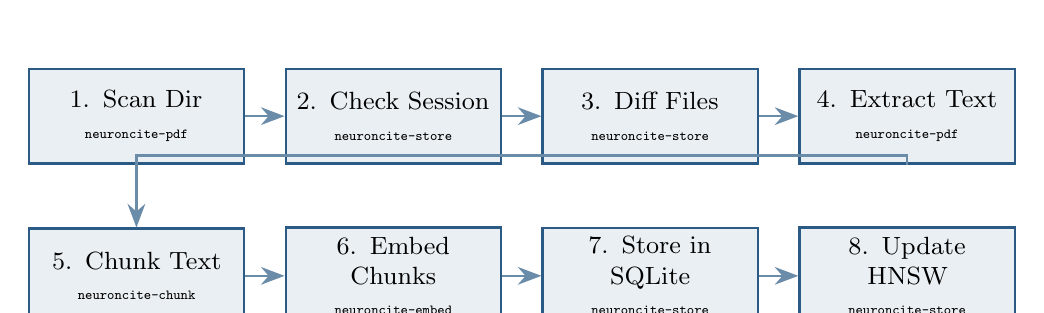
\begin{tikzpicture}[
    stage/.style={rectangle, draw=cratecolor, fill=cratecolor!10, thick,
                  minimum width=2.7cm, minimum height=1.2cm, text width=2.5cm,
                  align=center, font=\small},
    arrow/.style={-{Stealth[length=3mm]}, thick, color=cratecolor!70},
    node distance=0.5cm
]
    \node[stage] (s1) {1. Scan Dir\\{\tiny\texttt{neuroncite-pdf}}};
    \node[stage, right=of s1] (s2) {2. Check Session\\{\tiny\texttt{neuroncite-store}}};
    \node[stage, right=of s2] (s3) {3. Diff Files\\{\tiny\texttt{neuroncite-store}}};
    \node[stage, right=of s3] (s3b) {4. Extract Text\\{\tiny\texttt{neuroncite-pdf}}};
    \node[stage, below=0.8cm of s1] (s4) {5. Chunk Text\\{\tiny\texttt{neuroncite-chunk}}};
    \node[stage, right=of s4] (s5) {6. Embed Chunks\\{\tiny\texttt{neuroncite-embed}}};
    \node[stage, right=of s5] (s6) {7. Store in SQLite\\{\tiny\texttt{neuroncite-store}}};
    \node[stage, right=of s6] (s7) {8. Update HNSW\\{\tiny\texttt{neuroncite-store}}};

    \draw[arrow] (s1) -- (s2);
    \draw[arrow] (s2) -- (s3);
    \draw[arrow] (s3) -- (s3b);
    \draw[arrow] (s3b) |- ++(0,-0.5) -| (s4);
    \draw[arrow] (s4) -- (s5);
    \draw[arrow] (s5) -- (s6);
    \draw[arrow] (s6) -- (s7);
\end{tikzpicture}
\caption{The eight stages of the indexing pipeline. Stage 3 (Diff Files) compares the
         current directory contents against \texttt{indexed\_file} to identify new,
         modified, and deleted files. Unchanged files are skipped.}
\end{figure}

\begin{enumerate}[noitemsep]
    \item \textbf{Scan Directory:} Recursively discover all PDF files in the selected
          directory and its subdirectories.
    \item \textbf{Check Session:} Query the SQLite database for an existing
          \texttt{index\_session} with matching directory, model, and chunk configuration.
          If found, load the existing HNSW index and proceed to the incremental
          diff stage (step~3). If not, create a new session record and process all
          discovered files.
    \item {\begin{sloppypar}\textbf{Diff Against \texttt{indexed\_file}:} Compare the
          discovered file list against the \texttt{indexed\_file} table for this session.
          Classify each file as \textit{new} (not present in \texttt{indexed\_file}),
          \textit{modified} (\texttt{mtime} or \texttt{size} changed and SHA-256 hash
          differs), \textit{deleted} (present in \texttt{indexed\_file} but absent from
          the directory scan), or \textit{unchanged} (metadata matches). Delete the
          \texttt{indexed\_file} rows for deleted files (cascading to chunks and pages).
          For modified files, physically delete their old \texttt{page} and
          \texttt{chunk} rows (the \texttt{AFTER DELETE} trigger on \texttt{chunk}
          removes the corresponding FTS5 entries; the old HNSW vectors are temporary
          orphans until the graph rebuild in step~8).
          Skip unchanged files entirely.\end{sloppypar}}
    \item \textbf{Extract Text:} For each new or modified PDF file, extract text page by
          page using the configured backend (pdf-extract, pdfium, or auto with OCR
          fallback). Compute a SHA-256 hash of the file contents. Store extracted page
          text in the \texttt{page} table. Record or update the file in the
          \texttt{indexed\_file} table.
    \item \textbf{Chunk Text:} Apply the selected chunking strategy to the extracted pages,
          producing a list of \texttt{Chunk} values for each file. Each chunk records its
          document-level UTF-8 byte offsets and the page range it spans.
    \item \textbf{Embed Chunks:} Pass all chunk texts through the selected embedding backend
          in batches. The backend processes each batch on the GPU and returns the
          corresponding embedding vectors. Each vector is normalized to unit length.
    \item \textbf{Store in SQLite:} Write each chunk's text, metadata, and embedding blob
          to the \texttt{chunk} table and the FTS5 index. This is done in a single SQLite
          transaction for performance (bulk insert).
    \item \textbf{Update HNSW Index:} Build a new HNSW graph from all active embedding
          vectors of the session (existing chunks where \texttt{is\_deleted = 0}, plus
          the newly created chunks). The new graph is constructed on a background thread
          without affecting the current search index. Once the build completes, the
          session's entry in the per-session HNSW map is atomically replaced via
          \texttt{insert\_hnsw()}, and the old graph is dropped. This approach eliminates orphan accumulation for sessions
          that are re-indexed: each indexing run produces a clean graph. For sessions
          where files are only added (no deletions or modifications), the rebuild
          overhead is acceptable because the HNSW construction cost is dominated by the
          GPU embedding time that has already occurred. Serialize the graph to the
          session's index file in the \texttt{.neuroncite/} directory. Record the model
          manifest in \texttt{models.lock}.
\end{enumerate}

\subsection{Search Pipeline}

The search pipeline transforms a natural-language query into a ranked list of relevant
document passages with citations. It consists of five stages:

\begin{figure}[htbp]
\centering
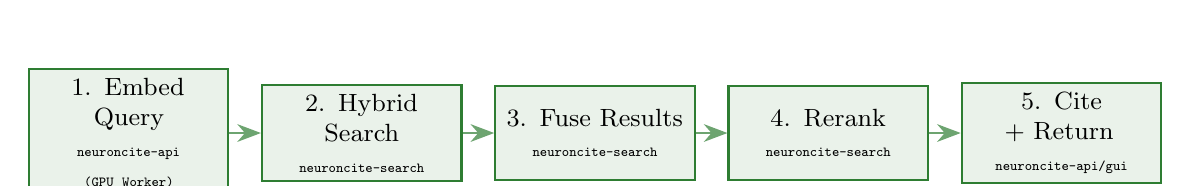
\begin{tikzpicture}[
    stage/.style={rectangle, draw=apicolor, fill=apicolor!10, thick,
                  minimum width=2.5cm, minimum height=1.2cm, text width=2.3cm,
                  align=center, font=\small},
    arrow/.style={-{Stealth[length=3mm]}, thick, color=apicolor!70},
    node distance=0.4cm
]
    \node[stage] (q1) {1. Embed Query\\{\tiny\texttt{neuroncite-api (GPU Worker)}}};
    \node[stage, right=of q1] (q2) {2. Hybrid Search\\{\tiny\texttt{neuroncite-search}}};
    \node[stage, right=of q2] (q3) {3. Fuse Results\\{\tiny\texttt{neuroncite-search}}};
    \node[stage, right=of q3] (q4) {4. Rerank\\{\tiny\texttt{neuroncite-search}}};
    \node[stage, right=of q4] (q5) {5. Cite + Return\\{\tiny\texttt{neuroncite-api/gui}}};

    \draw[arrow] (q1) -- (q2);
    \draw[arrow] (q2) -- (q3);
    \draw[arrow] (q3) -- (q4);
    \draw[arrow] (q4) -- (q5);
\end{tikzpicture}
\caption{The five stages of the search pipeline.}
\end{figure}

\begin{enumerate}[noitemsep]
    \item \textbf{Embed Query:} The query string is passed through the same embedding model
          that was used for indexing, producing a single query vector normalized to unit
          length.
    \item \textbf{Hybrid Search:} Two parallel searches are executed:
          \begin{itemize}[noitemsep]
              \item \textit{Vector:} The HNSW index is queried with the query vector,
                    returning the top $N_{\text{vec}}$ candidates with cosine similarity
                    scores.
              \item \textit{Keyword:} The FTS5 index is queried with the raw query string,
                    returning the top $N_{\text{kw}}$ candidates with BM25 scores.
          \end{itemize}
          If hybrid mode is disabled, only the vector search is executed.
    \item \textbf{Fuse Results:} The two candidate lists are merged using Reciprocal Rank
          Fusion (RRF). Candidates appearing in both lists receive a higher combined score.
          The top $K_{\text{rerank}}$ candidates proceed to the next stage.
    \item \textbf{Rerank (optional):} If a cross-encoder reranker is configured, the
          fused candidates are re-scored by jointly encoding each (query, chunk) pair.
          The reranker score replaces the RRF score as the primary ranking criterion.
          If no reranker is configured, this stage is skipped.
    \item \textbf{Cite and Return:} For each of the final top-K results, a
          \texttt{Citation} is generated from the chunk metadata (source file,
          page range, document-level byte offsets resolved to page-local positions
          via the \texttt{page.byte\_count} column). The \texttt{SearchResult} objects
          are returned to the GUI or API caller.
\end{enumerate}

\newpage

% ============================================================
% 12. CONCURRENCY MODEL
% ============================================================
\section{Concurrency Model}

The application must run an HTTP server, serve the web frontend, and potentially
long-running GPU computations simultaneously without blocking any of them.

\subsection{Thread Architecture}
\label{sec:thread-arch}

\begin{figure}[htbp]
\centering
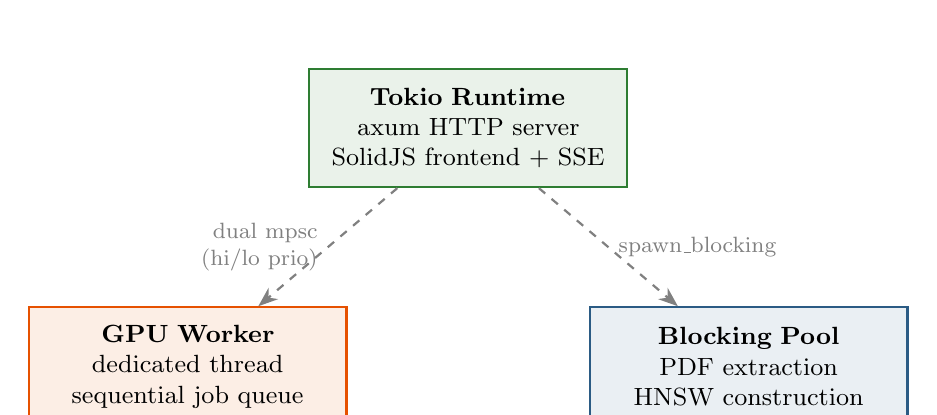
\begin{tikzpicture}[
    thread/.style={rectangle, draw=#1, fill=#1!10, thick, minimum width=4cm,
                   minimum height=1.5cm, text width=3.8cm, align=center, font=\small},
    comm/.style={-{Stealth[length=2.5mm]}, thick, dashed, color=black!50},
    node distance=2cm
]
    \node[thread=apicolor] (tokio) {\textbf{Tokio Runtime}\\axum HTTP server\\SolidJS frontend + SSE};
    \node[thread=storecolor, below left=1.5cm and -0.5cm of tokio] (gpu)
        {\textbf{GPU Worker}\\dedicated thread\\sequential job queue};
    \node[thread=cratecolor, below right=1.5cm and -0.5cm of tokio] (cpu)
        {\textbf{Blocking Pool}\\PDF extraction\\HNSW construction};

    \draw[comm] (tokio) -- node[left, font=\footnotesize, align=right] {dual mpsc\\(hi/lo prio)} (gpu);
    \draw[comm] (tokio) -- node[right, font=\footnotesize] {spawn\_blocking} (cpu);

\end{tikzpicture}
\caption{Thread architecture overview. The GPU Worker runs on a dedicated thread and
         processes embedding and reranking jobs from two channels (high-priority for
         search, low-priority for indexing).}
\end{figure}

\begin{description}[style=nextline]
    \item[Tokio Multi-Threaded Runtime]
        The tokio runtime hosts the axum HTTP server, serves the embedded SolidJS
        frontend, manages SSE broadcast channels for real-time updates, and
        coordinates all asynchronous background tasks (indexing, searching, model
        operations).

    \item[GPU Worker Thread]
        A single dedicated thread that owns the embedding backend and the reranker model.
        The thread is spawned and managed by the \texttt{worker} module in
        \texttt{neuroncite-api} (see \texttt{src/worker.rs} in the module structure
        table). It reads jobs from two separate bounded \texttt{tokio::sync::mpsc}
        channels---a high-priority channel for search-time jobs (query embedding,
        reranking) and a low-priority channel for indexing-time jobs (batch embedding).
        The worker's receive loop uses \texttt{tokio::select!} biased toward the
        high-priority channel: on each iteration it drains all pending high-priority
        jobs before polling the low-priority channel. This ensures that interactive
        queries are serviced with minimal latency even while a large indexing operation
        is in progress, without requiring a custom priority queue. Each job carries a
        oneshot response channel through which the GPU worker returns the result to the
        caller. The \texttt{WorkerHandle} struct provides the public interface
        (\texttt{embed\_query}, \texttt{embed\_batch}, \texttt{rerank\_batch}) that
        API handlers and web request handlers use to submit jobs. This architecture eliminates the
        need for a \texttt{Mutex} around the GPU resources: the worker thread is the
        sole owner, and all access is serialized through the handle's channels.

    \item[Blocking Thread Pool]
        CPU-bound operations (PDF text extraction, HNSW index construction, SHA-256
        hashing) are dispatched to tokio's blocking thread pool via
        \texttt{spawn\_blocking}. This prevents these operations from starving the async
        executor. GPU operations are not dispatched here -- they go through the dedicated
        GPU Worker Thread.
\end{description}

\textbf{Cancellation:} Each long-running job (batch embedding during indexing)
checks a \texttt{Cancellation\-Token} between batches. When the user cancels an
indexing operation through the GUI, the token is triggered, and the GPU worker
discards the remaining batches for that job. The cancellation is cooperative -- the
current batch runs to completion before the cancellation takes effect.

\subsection{Shared State Synchronization}

\begin{itemize}[noitemsep]
    \item \textbf{SQLite connection pool:} Managed by \texttt{r2d2}. The pool handles
          concurrent access internally. No additional application-level mutex is needed
          for database operations. WAL mode allows concurrent readers alongside a single
          writer. The \texttt{busy\_timeout} PRAGMA of 5000\,ms causes SQLite to sleep
          and retry internally when the write lock is held by another connection; if the
          lock is not released within 5000\,ms, SQLite returns \texttt{SQLITE\_BUSY}.
          The GUI treats a busy-timeout error as a transient condition and displays
          ``Database busy, retrying\ldots'' rather than a fatal error, retrying the
          operation up to three times with exponential backoff.
    \item \textbf{HNSW index map:} Stored in an
          \texttt{ArcSwap<HashMap<i64, Arc<HnswIndex>{>}{>}}. Each session has its
          own HNSW graph keyed by \texttt{session\_id}. Multiple search queries read
          the current map concurrently via a load of the \texttt{Arc} pointer
          (lock-free). Index construction and rebuilds build a new HNSW graph into a
          separate object without affecting the current map. Once the new graph is
          complete, the map is cloned, the session's entry is inserted, and the
          \texttt{ArcSwap} is atomically updated. Session deletion removes the entry
          from the map via \texttt{remove\_hnsw()} or \texttt{remove\_hnsw\_many()}.
          On startup, \texttt{load\_all\_session\_hnsw()} populates the map from
          all sessions with stored embeddings in the database.
    \item \textbf{Embedding backend and reranker:} Owned exclusively by the GPU Worker
          thread. No mutex is needed -- all access is mediated through the
          \texttt{WorkerHandle} interface (defined in
          \texttt{neuroncite-api/src/worker.rs}). The GUI and API call typed methods
          on the handle (\texttt{embed\_query}, \texttt{embed\_batch},
          \texttt{rerank\_batch}) and await the response on a oneshot channel. This
          avoids holding a \texttt{std::sync::Mutex} across \texttt{.await} points,
          which would risk deadlocks in the async context.
    \item \textbf{Index progress:} Reported through a \texttt{tokio::sync::watch} channel
          carrying \texttt{IndexProgress} values. The background task sends an updated
          progress snapshot after each file; the GUI calls \texttt{try\_recv()} on the
          watch receiver each frame to read the latest snapshot without blocking. The
          watch channel retains only the most recent value, making it suitable for
          high-frequency progress updates where intermediate values can be skipped.
\end{itemize}

\subsection{Graceful Shutdown}
\label{sec:graceful-shutdown}

The application implements a coordinated shutdown sequence that ensures data integrity
and releases resources in the correct order. Shutdown is triggered by three events:
(1)~closing the GUI window, (2)~sending \texttt{SIGINT} (Ctrl+C) or \texttt{SIGTERM}
to the process in headless mode, or (3)~calling \texttt{POST /api/v1/shutdown} (only
available in headless mode, protected by the bearer token when LAN binding is active).

\textbf{Shutdown sequence:}
\begin{enumerate}[noitemsep]
    \item The global \texttt{CancellationToken} is triggered, signaling all background
          tasks to stop accepting new work.
    \item The axum HTTP server stops accepting new connections and waits up to 5 seconds
          for in-flight requests to complete. After the grace period, remaining
          connections are dropped.
    \item The GPU Worker thread finishes its current batch (if any), then exits its job
          processing loop. No new jobs are accepted after the cancellation token fires.
    \item Any in-progress HNSW serialization completes. If serialization has not started
          for a modified graph, the system performs a final serialization to prevent
          data loss.
    \item The SQLite connection pool is drained: all checked-out connections are returned,
          pending WAL checkpoints are flushed, and the pool is closed.
    \item The tokio runtime shuts down, joining all spawned tasks.
    \item The process exits with code 0.
\end{enumerate}

\textbf{Forced shutdown:} If the graceful shutdown does not complete within 15 seconds,
the process exits with code 3. This timeout prevents indefinite hangs caused by
unresponsive GPU operations or stuck I/O.

\newpage

% ============================================================
% 13. FEATURE FLAGS
% ============================================================
\section{Cargo Feature Flags}

Feature flags control which embedding backends are compiled into the binary. This allows
users to build a minimal binary with only the backend they need, or a full binary with
all three.

\subsection{Feature Definitions}

Embedding backend features are defined on the \texttt{neuroncite-embed} crate and forwarded
through the workspace root and the binary crate. The \texttt{web}, \texttt{mcp},
\texttt{pdfium}, and \texttt{ocr} features are defined on the binary crate and
\texttt{neuroncite-pdf}, respectively.

\begin{table}[htbp]
\centering
\begin{tabularx}{\textwidth}{lX}
    \toprule
    \textbf{Feature} & \textbf{Effect} \\
    \midrule
    \texttt{backend-ort} (default) & Compiles the ONNX Runtime backend. Pulls in the
        \texttt{ort} and \texttt{ndarray} crates. Provides both embedding and
        reranking via ONNX models. Requires ONNX Runtime shared libraries at runtime
        for GPU execution. \\
    \texttt{web} (default) & Compiles the \texttt{neuroncite-web} crate and pulls in
        \texttt{rust-embed}, \texttt{mime\_guess}, and \texttt{opener}. Enables the
        \texttt{neuroncite web} CLI subcommand that starts an Axum server with the
        embedded SolidJS frontend and opens a native OS window (when the
        \texttt{gui} feature is also enabled) or the default browser. The
        \texttt{backend-ort} feature is forwarded to \texttt{neuroncite-web} via
        optional dependency syntax. Defined on the binary crate. \\
    \texttt{pdfium} (default) & Enables the \texttt{pdfium-render} backend in
        \texttt{neuroncite-pdf} for PDFs with multi-column layouts, complex tables,
        and non-standard font encodings. Requires the pdfium shared library at
        runtime. Defined on \texttt{neuroncite-pdf}, forwarded by the binary
        crate. \\
    \texttt{ocr} (default) & Enables Tesseract-based OCR fallback for image-heavy pages in
        \texttt{neuroncite-pdf}. Tesseract is invoked as a CLI subprocess and must
        be installed separately via the system package manager or the Doctor
        panel's install button. Implies the \texttt{pdfium} feature for page
        rendering to raster images. Defined on \texttt{neuroncite-pdf}, forwarded
        by the binary crate. \\
    \texttt{mcp} (default) & Compiles the \texttt{neuroncite-mcp} crate and enables the
        \texttt{mcp serve}, \texttt{mcp install}, \texttt{mcp uninstall}, and
        \texttt{mcp status} CLI subcommands. The MCP crate is an optional
        dependency of the binary crate (\texttt{dep:neuroncite-mcp}). When
        disabled, all MCP-related CLI subcommands are hidden and the binary
        has no MCP protocol code. The \texttt{backend-ort} feature is forwarded
        to \texttt{neuroncite-mcp} via the \texttt{neuroncite-mcp?/backend-ort}
        optional dependency syntax. Defined on the binary crate. \\
    \texttt{gui} (default) & Compiles the native OS window module in
        \texttt{neuroncite-web} using \texttt{tao} for the event loop and
        \texttt{wry} for the WebView. When enabled, the \texttt{web} subcommand
        opens a dedicated application window instead of a browser tab. The
        feature is forwarded from the binary crate to \texttt{neuroncite-web}
        via \texttt{neuroncite-web?/gui}. When disabled or when native window
        creation fails at runtime, the \texttt{opener}-based browser launch
        is used as fallback. Defined on \texttt{neuroncite-web}, forwarded by
        the binary crate. \\
    \bottomrule
\end{tabularx}
\caption{Feature flag definitions and their effects.}
\end{table}

\subsection{Build Commands}

\begin{table}[htbp]
\centering
\begin{tabularx}{\textwidth}{>{\raggedright\arraybackslash}p{0.52\textwidth}X}
    \toprule
    \textbf{Command} & \textbf{Result} \\
    \midrule
    \texttt{cargo build -{}-release} & Builds with default features (ort only). \\
    \texttt{cargo build -{}-release -{}-all-features} & Builds with all features enabled. \\
    \bottomrule
\end{tabularx}
\caption{Example build commands for different backend combinations.}
\end{table}

\subsection{Conditional Compilation}

Inside the \texttt{neuroncite-embed} crate, each backend module is wrapped in a
\texttt{\#[cfg(feature = "...")]} attribute. A backend registry function iterates over
all compiled-in backends and collects their \texttt{ModelInfo} lists. The GUI and API
only see backends that were actually compiled in.

\newpage

% ============================================================
% 14. ERROR HANDLING
% ============================================================
\section{Error Handling}

\subsection{Strategy}

The project follows the standard Rust error handling convention:

\begin{itemize}[noitemsep]
    \item \textbf{Library crates} (core, pdf, chunk, embed, store, search) use the
          \texttt{thiserror} crate to define typed error enumerations. Each crate has
          its own error type with variants for each failure mode.
    \item \textbf{Application crates} (api, gui, binary) use the \texttt{anyhow} crate
          for error aggregation, converting library errors into a unified error type
          with context messages.
\end{itemize}

\subsection{Error Propagation}

Library errors propagate upward through the \texttt{Result} type using the \texttt{?}
operator. At the API boundary, errors are mapped to appropriate HTTP status codes:

\begin{table}[htbp]
\centering
\begin{tabularx}{\textwidth}{lX}
    \toprule
    \textbf{Error Category} & \textbf{HTTP Status} \\
    \midrule
    Invalid request parameters & 400 Bad Request \\
    Session or resource not found & 404 Not Found \\
    Concurrent index job for the same session & 409 Conflict \\
    PDF extraction or embedding failure & 500 Internal Server Error \\
    \bottomrule
\end{tabularx}
\caption{Error-to-HTTP-status mapping.}
\end{table}

In the GUI, errors are displayed as dismissable notification banners at the top of the
results panel. The error message includes the error chain (original cause and context)
for debugging.

\newpage

% ============================================================
% 15. MODEL MANAGEMENT
% ============================================================
\section{Model Management}
\label{sec:model-mgmt}

The system downloads, caches, and tracks embedding and reranker models. Model management
ensures reproducibility (the same model version produces the same embeddings), supports
offline operation, and allows users to register locally stored models.

\subsection{Model Cache}

Model weights are cached in a platform-specific directory:
\begin{itemize}[noitemsep]
    \item \textbf{Windows:} \texttt{\%LOCALAPPDATA\%\textbackslash neuroncite\textbackslash models\textbackslash}
    \item \textbf{Linux:} \texttt{\textasciitilde/.cache/neuroncite/models/}
\end{itemize}

Each model is stored in a subdirectory named by its identifier and revision hash
(e.g., \texttt{BAAI--bge-small-en-v1.5--abc123/}). This allows multiple revisions of
the same model to coexist.

\subsection{Model Manifest (\texttt{models.lock})}

Each \texttt{.neuroncite/} directory contains a \texttt{models.lock} file that records the
exact model versions used to build the index. This file serves the same purpose as
\texttt{Cargo.lock}: it pins the model revision so that the index can be rebuilt
identically.

The manifest contains one entry per model used in the directory's index sessions.
Each entry records:
\begin{itemize}[noitemsep]
    \item \textbf{Model identifier:} The Hugging Face model ID (e.g.,
          ``BAAI/bge-small-en-v1.5'').
    \item \textbf{Revision:} The specific commit hash on Hugging Face Hub.
    \item \textbf{SHA-256 checksum:} Hash of the model weights file for integrity
          verification.
    \item \textbf{Tokenizer checksum:} SHA-256 hash of the tokenizer vocabulary file
          (\texttt{tokenizer.json}). The token-window chunking strategy depends on
          the tokenizer to produce deterministic chunk boundaries. Pinning the
          tokenizer checksum ensures that the same model revision with the same
          tokenizer always produces identical chunks, even if the tokenizer file is
          re-downloaded.
    \item \textbf{Source URL:} The URL from which the model was downloaded.
    \item \textbf{License:} The model's license identifier.
    \item \textbf{Local path:} Absolute path to the cached model directory on the machine
          that last wrote the manifest. This field is a diagnostic hint used to locate
          the model cache without re-scanning the file system. On a different machine,
          the application re-resolves the model by identifier and revision from the local
          cache directory, ignoring an invalid \texttt{local\_path}.
\end{itemize}

\subsection{Download and Verification}

On first use of a model, the system:
\begin{enumerate}[noitemsep]
    \item Resolves the latest revision from Hugging Face Hub (or uses a pinned revision
          if specified in \texttt{models.lock}).
    \item Downloads the model weights and tokenizer files.
    \item Computes the SHA-256 checksum and verifies it against the manifest (if present).
    \item Writes or updates the \texttt{models.lock} entry.
    \item Stores the files in the model cache directory.
\end{enumerate}

The download progress is shown in the GUI's progress bar.

\subsection{Offline Operation}

If the model is already cached, no network access is required. If the model is not
cached and the system is offline, the application displays an error message identifying
the missing model and its expected cache path, so the user can manually place the files.

\subsection{Local Model Registration}

Users can register locally stored model files (ONNX format)
through the GUI settings or the API. A registered model is added to the
\texttt{models.lock} manifest with a \texttt{file://} source URL and its computed
checksum. This enables use of custom or proprietary models without requiring Hugging
Face Hub access.

\newpage

% ============================================================
% 16. BUILD AND DEPLOYMENT
% ============================================================
\section{Build and Deployment}

\subsection{Build Output}

The final build artifact is a single executable file. On Windows, this is
\texttt{neuroncite.exe}. The binary contains:

\begin{itemize}[noitemsep]
    \item The SolidJS web frontend (embedded via rust-embed, served by axum)
    \item The axum HTTP server
    \item The SQLite engine (statically linked via rusqlite's bundled feature)
    \item The HNSW index implementation
    \item The selected embedding backend(s) and reranker(s)
    \item All tokenizer vocabularies (embedded as assets or downloaded on first use)
\end{itemize}

\subsection{Runtime Dependencies}
\label{sec:runtime-deps}

The runtime dependencies depend on the build configuration:

\begin{table}[htbp]
\centering
\begin{tabularx}{\textwidth}{lX}
    \toprule
    \textbf{Configuration} & \textbf{Runtime Requirements} \\
    \midrule
    CPU-only (any backend, \texttt{pdf-extract} only) & None for the core
        embedding and search pipeline. GPU acceleration is unavailable, but all
        core functionality works on CPU. PDFium and Tesseract dependencies are
        listed separately below and apply regardless of CPU or GPU mode. \\
    \texttt{backend-ort} + GPU & ONNX Runtime shared libraries (\texttt{onnxruntime.dll}
        / \texttt{libonnxruntime.so}), NVIDIA CUDA toolkit, and cuDNN. \\
    PDF extraction (pdfium) & PDFium shared library (\texttt{pdfium.dll} /
        \texttt{libpdfium.so}). Required if the pdfium extraction backend is used
        \textbf{or} if OCR fallback is enabled (OCR uses pdfium for page-to-image
        rendering). \\
    OCR & Tesseract OCR engine, trained language data files, \textbf{and} the PDFium
        shared library (for page rendering). Only required if OCR fallback is
        triggered. \\
    \bottomrule
\end{tabularx}
\caption{Runtime dependencies by configuration.}
\end{table}

\subsection{Distribution Profiles}

The ``single binary'' claim holds for the CPU-only build, but GPU-enabled builds and
PDF extraction via pdfium require external shared libraries. To prevent user confusion,
the project defines four explicit distribution profiles:

\begin{table}[htbp]
\centering
\begin{tabularx}{\textwidth}{lX}
    \toprule
    \textbf{Profile} & \textbf{Contents and Dependencies} \\
    \midrule
    \textbf{Portable CPU} & A single \texttt{neuroncite.exe} (or \texttt{neuroncite} on Linux)
        with no external dependencies. All processing runs on CPU. Embedding inference is
        slower but fully self-contained. Suitable for machines without a GPU. \\
    \textbf{GPU NVIDIA (ort)} & The binary plus bundled ONNX Runtime shared libraries
        (\texttt{onnxruntime.dll} / \texttt{libonnxruntime.so}) and a cuDNN redistribution.
        Requires the NVIDIA CUDA toolkit to be installed on the system. Distributed as a
        ZIP archive with a directory layout that places all DLLs alongside the binary. \\
    \bottomrule
\end{tabularx}
\caption{Distribution profiles. Each profile targets a specific hardware and dependency
         configuration.}
\end{table}

All profiles optionally include PDFium (\texttt{pdfium.dll} / \texttt{libpdfium.so})
for the pdfium extraction backend and Tesseract language data files for OCR. These
optional components are detected at runtime, and missing components degrade gracefully
(fallback to \texttt{pdf-extract} or skipping OCR).

\subsection{Dependency Doctor}

The GUI includes a \textbf{Dependency Doctor} panel accessible from the settings menu.
On application startup, and on demand through a ``Check Dependencies'' button, the
system probes for all optional runtime dependencies and reports their status:

\begin{itemize}[noitemsep]
    \item \textbf{CUDA toolkit:} Checks for \texttt{nvcc} on the system PATH and reports
          the detected version. If missing, displays the NVIDIA download URL.
    \item \textbf{cuDNN:} Checks for \texttt{cudnn64\_8.dll} (Windows) or
          \texttt{libcudnn.so} (Linux) in the library search path. Reports version if
          found.
    \item \textbf{ONNX Runtime:} Checks for \texttt{onnxruntime.dll} /
          \texttt{libonnxruntime.so} adjacent to the binary or on the library path.
          If missing and the ort backend is compiled in, offers a download button that
          fetches the correct version from the ONNX Runtime GitHub releases.
    \item \textbf{PDFium:} Checks for \texttt{pdfium.dll} / \texttt{libpdfium.so}
          adjacent to the binary. If missing, offers a download button that fetches the
          library from the pdfium-binaries GitHub releases.
    \item \textbf{Tesseract:} Checks for the \texttt{tesseract} binary on the system
          PATH and for the \texttt{TESSDATA\_PREFIX} environment variable. Reports
          available language data files.
    \item \textbf{GPU driver:} Queries the GPU vendor and driver version via the
          platform's graphics API (DXGI on Windows, Vulkan on Linux). Reports whether
          the driver is compatible with the compiled-in backends.
\end{itemize}

Each dependency displays one of three states: ``Found (version X.Y)'', ``Missing
(required for Z)'', or ``Not needed (feature not compiled in)''. Missing dependencies
that have a known download source display an actionable download button.

\subsection{Continuous Integration}

A CI pipeline builds and tests the application across a matrix of:
\begin{itemize}[noitemsep]
    \item Operating systems: Windows, Linux
    \item Feature combinations: ort-only, all-features
    \item Rust toolchain: stable
\end{itemize}

Tests run with the CPU execution provider to avoid requiring GPU hardware in CI.

\newpage

% ============================================================
% 17. CLI INTERFACE
% ============================================================
\section{Command-Line Interface}
\label{sec:cli}

The binary supports a set of subcommands parsed by the \texttt{clap} crate. When the
binary is invoked without any subcommand, it defaults to web mode (equivalent to
\texttt{neuroncite web}). All subcommands that produce output write machine-readable
JSON to stdout by default. A \texttt{-{}-format text} flag switches to human-readable
tabular output for interactive terminal use.

\subsection{Subcommands}

\begin{table}[htbp]
\centering
\begin{tabularx}{\textwidth}{>{\ttfamily\raggedright\arraybackslash}p{3cm}X}
    \toprule
    \normalfont\textbf{Subcommand} & \textbf{Description} \\
    \midrule
    web             & Starts the Axum HTTP server with the embedded SolidJS
                      frontend and opens a native OS window (with the \texttt{gui}
                      feature) or the default browser (without \texttt{gui}). This
                      is the default mode when no subcommand is given (double-click
                      behavior on Windows). Accepts \texttt{-{}-port}, \texttt{-{}-bind},
                      and \texttt{-{}-config} flags. \\
    serve           & Starts the API server in headless mode without a browser window.
                      The server runs until terminated by \texttt{SIGINT} (Ctrl+C),
                      \texttt{SIGTERM}, or a \texttt{/api/v1/shutdown} request.
                      Accepts \texttt{-{}-port}, \texttt{-{}-bind},
                      \texttt{-{}-print-token}, and \texttt{-{}-config} flags. \\
    index           & Indexes a directory from the command line without starting a
                      persistent HTTP server. Internally, this subcommand spawns a
                      tokio runtime and initializes the embedding backend (including
                      GPU resources if available) for the duration of the indexing
                      operation; both are torn down on completion. Accepts
                      \texttt{-{}-directory}, \texttt{-{}-model},
                      \texttt{-{}-strategy}, \texttt{-{}-chunk-size},
                      \texttt{-{}-overlap}, and \texttt{-{}-ocr-language} flags.
                      Outputs a JSON object with the \texttt{session\_id} and
                      indexing statistics on completion. \\
    search          & Executes a single search query against an existing session.
                      Accepts \texttt{-{}-directory}, \texttt{-{}-session-id},
                      \texttt{-{}-query}, \texttt{-{}-top-k}, \texttt{-{}-hybrid},
                      and \texttt{-{}-rerank} flags. Outputs a JSON array of
                      \texttt{SearchResult} objects. \\
    doctor          & Runs the Dependency Doctor checks and reports the status of
                      all optional runtime dependencies (CUDA, cuDNN, ONNX Runtime,
                      PDFium, Tesseract, GPU driver). Outputs a JSON object with
                      each dependency's status. \\
    sessions        & Lists all index sessions in the specified directory's
                      \texttt{.neuroncite/} database. Accepts a
                      \texttt{-{}-directory} flag. Outputs a JSON array of session
                      summary objects. \\
    export          & Exports search results from a previous search to Markdown,
                      BibTeX, or CSL-JSON. Accepts \texttt{-{}-directory},
                      \texttt{-{}-session-id}, \texttt{-{}-query},
                      \texttt{-{}-format} (markdown, bibtex, csl-json), and
                      \texttt{-{}-output} (file path, defaults to stdout). \\
    annotate        & Runs the PDF annotation pipeline from the command line.
                      Accepts \texttt{-{}-input} (CSV or JSON quote file),
                      \texttt{-{}-pdf} (source PDF path), and
                      \texttt{-{}-output} (annotated PDF path) flags.
                      Outputs a JSON object with the annotation results on
                      completion. \\
    models          & Model management subcommand group for LLM agent control.
                      Provides five nested subcommands (\texttt{list},
                      \texttt{info}, \texttt{download}, \texttt{verify},
                      \texttt{system}) that expose the embedding model catalog,
                      cache status, download operations, integrity verification,
                      and GPU/system capability detection. All output is
                      machine-readable JSON by default. See
                      Section~\ref{sec:cli-models} for the full schema. \\
    mcp             & MCP server management subcommand group. Provides four
                      nested subcommands: \texttt{serve} (start the MCP stdio
                      server), \texttt{install} (register in Claude Code MCP
                      settings), \texttt{uninstall} (remove registration),
                      and \texttt{status} (report registration status). \\
    version         & Prints the application version, build features, and Git
                      commit hash as a JSON object (or a single line in text
                      format). \\
    \bottomrule
\end{tabularx}
\caption{CLI subcommands. All subcommands support the global flags
         \texttt{-{}-format} (json or text), \texttt{-{}-config} (path to
         configuration file), and \texttt{-{}-log-level} (trace, debug, info, warn,
         error).}
\end{table}

\subsection{Exit Codes}

\begin{table}[htbp]
\centering
\begin{tabularx}{\textwidth}{lX}
    \toprule
    \textbf{Code} & \textbf{Meaning} \\
    \midrule
    0 & The operation completed successfully. \\
    1 & Application error (indexing failure, search failure, database error, GPU
        initialization failure). The error message is written to stderr as a JSON
        object with \texttt{error} and \texttt{code} fields. \\
    2 & Usage error (invalid arguments, missing required flags, unknown subcommand).
        Printed by clap with a help message. \\
    3 & Shutdown timeout (the graceful shutdown did not complete within 15 seconds). \\
    \bottomrule
\end{tabularx}
\caption{CLI exit codes. Scripts and agents can rely on these codes for control flow.}
\end{table}

\subsection{JSON Output Contract}

CLI subcommands that correspond to API endpoints produce JSON output matching the API
response schema where the semantics are equivalent. For example, the output of
\texttt{neuroncite search} matches the response body of \texttt{POST /api/v1/search},
and \texttt{neuroncite doctor} matches \texttt{GET /api/v1/health}. The
\texttt{neuroncite index} subcommand is an exception: because it runs synchronously
(blocking until indexing completes), its output is a completion result containing
\texttt{session\_id}, \texttt{chunks\_created}, \texttt{files\_processed}, and
\texttt{elapsed\_seconds}---not the asynchronous \texttt{job\_id} response returned
by \texttt{POST /api/v1/index}. Clients switching between CLI and API invocation must
account for this difference in the index operation.

Progress output (during \texttt{neuroncite index}) is written to stderr as newline-
delimited JSON (NDJSON) objects, one per processed file. This separation ensures that
stdout contains only the final result object, while stderr provides real-time progress
updates that can be consumed by monitoring tools or discarded.

Two flags control progress output behavior:

\begin{itemize}[noitemsep]
    \item \texttt{-{}-quiet} -- suppresses all stderr progress output. Only the final
          JSON result is written to stdout. Useful for scripts that do not need
          progress reporting and want to avoid parsing or redirecting stderr.
    \item \texttt{-{}-progress} \textit{mode} -- selects the progress output format.
          Accepted values: \texttt{ndjson} (default, one JSON object per file on
          stderr) and \texttt{none} (equivalent to \texttt{-{}-quiet}). Future
          versions may add additional formats (e.g., a compact single-line counter).
\end{itemize}

\noindent When \texttt{-{}-quiet} is combined with \texttt{-{}-progress ndjson}, the
\texttt{-{}-quiet} flag takes precedence and progress output is suppressed.

\subsection{Model Management Subcommands}
\label{sec:cli-models}

The \texttt{neuroncite models} subcommand group provides LLM agents and automation
scripts with programmatic access to the embedding model catalog, local cache state,
download operations, integrity verification, and GPU/system capability detection. All
five nested subcommands produce JSON to stdout by default and write errors to stderr
as JSON objects with \texttt{error} and \texttt{code} fields.

\subsubsection{\texttt{models list}}

Lists all supported embedding models with their configuration parameters and local
cache status. The JSON output contains a \texttt{models} array where each entry
includes \texttt{model\_id}, \texttt{display\_name}, \texttt{vector\_dimension},
\texttt{max\_seq\_len}, \texttt{pooling} (one of ``cls'', ``mean-pooling'',
``last-token''), \texttt{uses\_token\_type\_ids}, \texttt{query\_prefix},
\texttt{document\_prefix}, \texttt{cached} (boolean), and \texttt{cache\_path}
(present only when cached). Two summary fields \texttt{total} and
\texttt{cached\_count} provide the aggregate counts. The invariant
\texttt{cached\_count $\leq$ total} always holds.

\subsubsection{\texttt{models info <model-id>}}

Returns the full configuration and per-file status for a single model identified
by its Hugging Face model ID (e.g., \texttt{BAAI/bge-small-en-v1.5}). In addition
to the fields from \texttt{models list}, the response includes a \texttt{files}
array listing each expected file with \texttt{filename}, \texttt{exists} (boolean),
and \texttt{size\_bytes} (present only when the file exists). If the model ID is
not in the catalog, the command exits with code~1 and writes a JSON error object
with \texttt{code} set to \texttt{model\_not\_found}.

\subsubsection{\texttt{models download <model-id>}}

Downloads the model files from Hugging Face Hub to the local cache. If the model
is already cached, the command returns immediately with \texttt{status} set to
\texttt{already\_cached}. For a fresh download, the response includes
\texttt{status} set to \texttt{downloaded}, the \texttt{cache\_path}, and
\texttt{elapsed\_seconds} measuring the wall-clock download time. Download progress
is written to stderr. An unknown model ID produces exit code~1 with a
\texttt{model\_not\_found} error.

\subsubsection{\texttt{models verify <model-id>}}

Checks file existence and computes SHA-256 checksums for all expected files of the
specified model. The response contains a \texttt{files} array with per-file
\texttt{filename}, \texttt{exists}, and \texttt{sha256} (present when the file
exists) fields. A top-level \texttt{valid} boolean is \texttt{true} only when all
expected files exist. An unknown model ID produces exit code~1.

\subsubsection{\texttt{models system}}

Reports system capabilities relevant to embedding model execution. The response
contains a \texttt{gpu} object with three detection layers: \texttt{nvidia\_detected}
(whether an NVIDIA GPU is present, detected via \texttt{nvidia-smi}),
\texttt{cuda\_available} (whether the ONNX Runtime CUDA execution provider can
initialize), and \texttt{gpu\_ort\_runtime} (whether the locally cached ORT
runtime DLL was built with GPU support). A \texttt{backends} array lists the
compiled-in embedding backend names. The \texttt{cache\_dir} field provides the
absolute path to the model cache directory, and
\texttt{cache\_disk\_usage\_bytes} reports the total disk usage of all cached
models. This information enables agents to determine whether GPU acceleration is
available before initiating indexing operations.

\newpage

% ============================================================
% 18. OPERATIONAL CONCERNS
% ============================================================
\section{Operational Concerns}
\label{sec:operational}

\subsection{Configuration File}

Application-wide settings are stored in a TOML configuration file. The configuration
file is loaded from the following locations in order of precedence (first found wins):

\begin{enumerate}[noitemsep]
    \item Path specified by the \texttt{-{}-config} CLI flag
    \item Path specified by the \texttt{NEURONCITE\_CONFIG} environment variable
    \item \texttt{.neuroncite/config.toml} in the current working directory
    \item Platform-specific user configuration directory:
    \begin{itemize}[noitemsep]
        \item Windows: \texttt{\%APPDATA\%\textbackslash neuroncite\textbackslash config.toml}
        \item Linux: \texttt{\textasciitilde/.config/neuroncite/config.toml}
    \end{itemize}
\end{enumerate}

If no configuration file is found, the application uses built-in defaults. CLI flags
and environment variables override the corresponding configuration file values.

\textbf{Configuration fields:}
\begin{table}[htbp]
\centering
\begin{tabularx}{\textwidth}{>{\ttfamily\raggedright\arraybackslash}p{3.8cm}
                              >{\raggedright\arraybackslash}p{2cm}X}
    \toprule
    \normalfont\textbf{Field} & \textbf{Type} & \textbf{Description} \\
    \midrule
    port                & integer & API server port (default: 3030). \\
    bind\_address       & string  & Bind address (default: ``127.0.0.1''). \\
    log\_level          & string  & Minimum log level for stderr output: trace,
                          debug, info, warn, error. Default: ``info'' in
                          headless mode, ``warn'' in GUI mode (to avoid
                          cluttering the terminal that launched the
                          application). An explicit value in the config file
                          or \texttt{-{}-log-level} CLI flag overrides the
                          mode-specific default. \\
    log\_file           & string  & Path to log file. If set, logs are written to
                          this file in addition to stderr (default: null, no file
                          logging). \\
    default\_model      & string  & Default embedding model identifier
                          (default: ``BAAI/bge-small-en-v1.5''). \\
    default\_strategy   & string  & Default chunking strategy (default: ``word''). \\
    default\_chunk\_size & integer & Default chunk size (default: 300). \\
    default\_overlap    & integer & Default chunk overlap (default: 50). \\
    ocr\_language       & string  & Default Tesseract language (default: ``eng''). \\
    ef\_search          & integer & Default HNSW ef\_search parameter
                          (default: 100). \\
    rrf\_k              & integer & Default RRF fusion parameter $k$
                          (default: 60). \\
    cors\_origins        & array   & TOML array of allowed CORS origin strings for
                          LAN mode (e.g.,
                          \texttt{["http://192.168.1.0:3000"]}). If empty or
                          unset, all origins are allowed via wildcard. Ignored
                          when bound to localhost (default: \texttt{[]}). \\
    simhash\_threshold  & integer & Maximum Hamming distance (out of 64 bits)
                          below which two chunks are considered
                          near-duplicates during deduplication
                          (default: 3). \\
    orphan\_ratio\_\allowbreak threshold
                        & float   & HNSW orphan ratio above which a rebuild is
                          recommended (default: 0.2). \\
    \bottomrule
\end{tabularx}
\caption{Configuration file fields with their types and defaults.}
\end{table}

\subsection{Logging}

The application uses the \texttt{tracing} crate for structured, leveled logging.
Log output is configured as follows:

\begin{itemize}[noitemsep]
    \item \textbf{Stderr:} In both GUI and headless mode, log messages at the
          configured level and above are written to stderr in a human-readable
          format (\texttt{tracing-subscriber} compact formatter). In GUI mode, the
          log level defaults to \texttt{warn} to avoid cluttering the terminal that
          launched the application. In headless mode, the default level is
          \texttt{info}.
    \item \textbf{Log file:} When the \texttt{log\_file} configuration field is set
          or the \texttt{-{}-log-file} CLI flag is provided, log messages are
          additionally written to the specified file in JSON format (one JSON object
          per log event). The log file uses append mode and is safe for concurrent
          writes from multiple threads. Log rotation is left to external tools
          (e.g., \texttt{logrotate} on Linux).
    \item \textbf{GUI log panel:} In GUI mode, the last 500 log messages at
          \texttt{info} level and above are displayed in a scrollable log panel
          accessible from the settings menu. This enables diagnosing issues without
          leaving the application.
\end{itemize}

\textbf{Log fields:} Each log event includes the timestamp (ISO 8601), level, target
module, thread name, span context (e.g., the current job ID or file being processed),
and the message. Sensitive data (bearer tokens, file system paths containing
usernames) is redacted in log output.

\subsection{Storage Location for Operational Files}

\begin{table}[htbp]
\centering
\begin{tabularx}{\textwidth}{lX}
    \toprule
    \textbf{File} & \textbf{Location} \\
    \midrule
    Database and HNSW index files & \texttt{<base>/indexes/<sanitized-path>/}.
                  Storage is centralized under a single root directory
                  (\texttt{<base>}), not inside the indexed directory itself.
                  The path sanitization converts absolute paths to flat names
                  (e.g., \texttt{D:\textbackslash Papers\textbackslash Finance}
                  becomes \texttt{D\_-{}-Papers-{}-Finance}). \\
    Base directory (\texttt{<base>}) &
                  \textbf{Windows:} \texttt{\%APPDATA\%\textbackslash NeuronCite}
                  (fallback: \texttt{\%USERPROFILE\%\textbackslash Documents\textbackslash
                  NeuronCite}).
                  \textbf{Linux:} \texttt{\$XDG\_DATA\_HOME/NeuronCite}
                  (fallback: \texttt{\textasciitilde/Documents/NeuronCite}).
                  \textbf{macOS:} \texttt{\textasciitilde/Documents/NeuronCite}. \\
    Runtime dependencies & \texttt{<base>/runtime/} (ONNX Runtime DLLs, pdfium
                  shared library, Tesseract executable and tessdata). \\
    Model cache & \texttt{<base>/models/} (downloaded ONNX embedding and
                  reranker model files from HuggingFace). \\
    Configuration file & User-specified via \texttt{-{}-config <path>} CLI flag.
                  No default location; \texttt{AppConfig::default()} is used
                  when no file is provided. The file format is TOML. \\
    Log file (if configured) & User-specified path. \\
    Bearer token (LAN mode) & Generated at runtime and printed to stdout when
                  \texttt{-{}-print-token} is passed to \texttt{neuroncite serve}.
                  Not persisted to disk. \\
    Export files & \texttt{<base>/indexes/<sanitized-path>/exports/}. \\
    \bottomrule
\end{tabularx}
\caption{File system locations for operational files. All paths are relative to
         the centralized base directory (\texttt{<base>}) resolved by
         \texttt{neuroncite\_core::paths::base\_dir()}.}
\end{table}

\newpage

% ============================================================
% 19. AGENT INTEGRATION AND PYTHON CLIENT
% ============================================================
\section{Agent Integration and Python Client}
\label{sec:agent-integration}

The application is designed to be operated by automated agents (LLM-based or
script-based) in addition to human users. This section describes the integration
contract and the reference Python client.

\subsection{Integration Modes}

An automated agent can interact with NeuronCite through four interfaces, ordered
by recommendation:

\begin{enumerate}[noitemsep]
    \item \textbf{MCP stdio server (recommended for Claude Code):} The agent runtime
          spawns \texttt{neuroncite mcp serve} as a subprocess and communicates
          via JSON-RPC 2.0 over stdin/stdout. Claude Code auto-starts the MCP
          server based on the registration entry in
          \texttt{\textasciitilde/.claude/claude\_mcp\_settings.json}. This mode
          provides the tightest integration with AI assistants that support the
          Model Context Protocol.
    \item \textbf{HTTP API (recommended for general use):} The agent starts the
          server via \texttt{neuroncite serve} (or relies on an already-running
          instance) and sends HTTP requests to
          \texttt{http://127.0.0.1:3030/api/v1/}. This mode supports concurrent
          operations, job tracking, and long-lived sessions.
    \item \textbf{CLI subcommands:} The agent invokes \texttt{neuroncite index},
          \texttt{neuroncite search}, etc. as subprocess calls and parses the
          JSON output from stdout. This mode requires no running server and is
          suitable for one-shot operations in pipelines.
    \item \textbf{Python client library:} A thin Python wrapper around the HTTP API
          that provides typed method signatures and handles server lifecycle
          management.
\end{enumerate}

\subsection{Server Lifecycle for Agents}

Agents that use the HTTP API need a running server. The recommended pattern:

\begin{enumerate}[noitemsep]
    \item Start the server as a subprocess:
          \texttt{neuroncite serve -{}-port 3030}
    \item Wait for the server to become ready by polling
          \texttt{GET /api/v1/health} until it returns HTTP 200.
    \item Perform indexing and search operations via the API.
    \item Shut down the server by sending \texttt{SIGINT} to the subprocess or (if
          in headless mode) by calling \texttt{POST /api/v1/shutdown}.
\end{enumerate}

The Python client library automates this lifecycle (see below).

\subsection{Python Client Library}

The repository contains a reference Python client in the \texttt{clients/python/}
directory, installable via \texttt{pip install -e clients/python/}. The client
provides a minimal, typed interface for all API operations.

\textbf{Client architecture:}

\begin{itemize}[noitemsep]
    \item \textbf{Class \texttt{NeuronCiteClient}:} Wraps all HTTP API calls. Accepts
          \texttt{base\_url} (default: \texttt{http://127.0.0.1:3030}) and an optional
          \texttt{token} for LAN-mode authentication. 33 public methods organized
          by domain:
          \begin{itemize}[noitemsep, topsep=2pt]
              \item \textbf{System:} \texttt{health()}, \texttt{backends()},
                    \texttt{shutdown()}.
              \item \textbf{Indexing:} \texttt{index()}.
              \item \textbf{Search:} \texttt{search()}, \texttt{hybrid\_search()},
                    \texttt{multi\_search()}.
              \item \textbf{Verification:} \texttt{verify()}.
              \item \textbf{Jobs:} \texttt{get\_job()}, \texttt{wait\_for\_job()},
                    \texttt{cancel\_job()}, \texttt{list\_jobs()}.
              \item \textbf{Sessions:} \texttt{list\_sessions()},
                    \texttt{delete\_session()},
                    \texttt{delete\_sessions\_by\_directory()},
                    \texttt{optimize\_session()}, \texttt{rebuild\_index()}.
              \item \textbf{Documents:} \texttt{get\_page()},
                    \texttt{quality\_report()}, \texttt{compare\_files()},
                    \texttt{discover()}.
              \item \textbf{Annotation:} \texttt{annotate()},
                    \texttt{annotate\_from\_file()}.
              \item \textbf{Citation:} \texttt{citation\_create()},
                    \texttt{citation\_claim()}, \texttt{citation\_submit()},
                    \texttt{citation\_status()}, \texttt{citation\_rows()},
                    \texttt{citation\_export()},
                    \texttt{citation\_auto\_verify()},
                    \texttt{citation\_fetch\_sources()},
                    \texttt{citation\_parse\_bib()},
                    \texttt{citation\_bib\_report()}.
          \end{itemize}
    \item \textbf{Class \texttt{NeuronCiteServer}:} Manages the server subprocess.
          The constructor accepts the path to the \texttt{neuroncite} binary and
          optional configuration (port, bind address, log level). The
          \texttt{start()} method launches the subprocess and blocks until the health
          endpoint responds. The \texttt{stop()} method sends \texttt{SIGINT} and waits
          for the process to exit. Implements the context manager protocol
          (\texttt{\_\_enter\_\_}/\texttt{\_\_exit\_\_}) for use in \texttt{with}
          statements.
    \item \textbf{Data classes:} Typed dataclasses defined in the
          \texttt{neuroncite.models} module for all response structures
          (\texttt{IndexResponse}, \texttt{SearchResult}, \texttt{JobStatus},
          \texttt{HealthResponse}, \texttt{CitationCreateResponse}, etc.).
          These mirror the Rust DTOs in \texttt{neuroncite-api/src/dto.rs}.
\end{itemize}

\textbf{Usage example:}

\begin{designbox}[Python Client Usage]
\begin{verbatim}
from neuroncite import NeuronCiteServer, NeuronCiteClient

with NeuronCiteServer("./neuroncite.exe", port=3030) as server:
    client = NeuronCiteClient(base_url=server.url)

    # Index a directory
    job = client.index(
        directory="C:/papers/econometrics",
        model="BAAI/bge-small-en-v1.5",
        chunk_strategy="word",
        chunk_size=300,
        overlap=50,
    )
    result = client.wait_for_job(job.job_id)

    # Search
    results = client.search(
        session_id=result.session_id,
        query="financial econometrics methodology",
        top_k=5,
    )
    for r in results:
        print(r.citation.formatted)
\end{verbatim}
\end{designbox}

\subsection{OpenAPI Specification}

The OpenAPI 3.1 specification is served at \texttt{GET /api/v1/openapi.json} and is
generated at compile time from the Rust handler type signatures using the
\texttt{utoipa} crate. The specification describes all endpoints, request bodies,
response schemas, and error responses. Agents can use this specification to
auto-generate client bindings in any language, validate requests before sending them,
or feed the specification to an LLM as context for tool-use prompting.

The specification file is also checked into the repository at
\texttt{docs/openapi.json} for offline reference and CI-based schema validation.

\subsection{LLM Agent Tool-Use Contract}

For LLM agents that use function-calling or tool-use interfaces, each API endpoint
maps to a single tool definition. The tool descriptions, parameter schemas, and
return value schemas are derived from the OpenAPI specification. The recommended
approach is to provide the LLM with the OpenAPI specification as context and let
the LLM construct HTTP requests directly.

\textbf{Key design decisions for agent compatibility:}
\begin{itemize}[noitemsep]
    \item All responses are flat JSON objects or arrays (no nested pagination
          wrappers). Agents can iterate over results directly.
    \item Enumerated string fields (e.g., job state, chunk strategy) use
          lowercase snake\_case identifiers that are unambiguous and
          copy-paste-safe.
    \item Error responses include a machine-readable \texttt{code} field (e.g.,
          ``session\_not\_found'', ``index\_in\_progress'') that agents can
          match against without parsing human-readable error messages.
    \item The \texttt{/api/v1/health} endpoint returns enough information for
          an agent to determine which features are available before attempting
          to use them.
    \item The \texttt{neuroncite models} CLI subcommand group
          (Section~\ref{sec:cli-models}) provides agents with model catalog
          discovery, cache status, download control, integrity verification,
          and GPU capability detection without requiring a running HTTP server.
          Agents that operate in CLI-only mode (no \texttt{serve} process) can
          use these subcommands to inspect and prepare the embedding environment
          before executing \texttt{index} or \texttt{search} operations.
\end{itemize}

\newpage

% ============================================================
% 20. MODEL CONTEXT PROTOCOL (MCP) SERVER
% ============================================================
\section{Model Context Protocol Server}
\label{sec:mcp-server}

The \texttt{neuroncite-mcp} crate implements a Model Context Protocol server that
enables AI assistants (Claude Code, and other MCP-compatible clients) to access all
NeuronCite operations through a standardized tool-use interface. The server
communicates via JSON-RPC 2.0 over stdin/stdout, following the MCP specification
version derived from the workspace crate version (\texttt{CARGO\_PKG\_VERSION}).

\subsection{Protocol Architecture}

The MCP server processes requests through a layered pipeline:

\begin{enumerate}[noitemsep]
    \item \textbf{Transport layer} (\texttt{transport.rs}): Reads complete JSON lines
          from stdin via \texttt{StdioReader} and writes serialized responses to
          stdout via \texttt{StdioWriter}. All diagnostic logging is directed to
          stderr to keep the stdout channel clean for protocol messages.
    \item \textbf{Protocol layer} (\texttt{protocol.rs}): Defines the JSON-RPC 2.0
          message types. \texttt{JsonRpcRequest} contains the method name, params
          object, and request ID. \texttt{JsonRpcResponse} wraps either a result
          value or a \texttt{JsonRpcError} with code and message fields.
    \item \textbf{Server loop} (\texttt{server.rs}): Drives the request lifecycle.
          Performs the MCP \texttt{initialize} handshake (exchanging protocol
          version and server capabilities), responds to \texttt{tools/list} with
          the tool catalog, dispatches \texttt{tools/call} requests to handlers,
          and handles \texttt{notifications/cancelled} messages.
    \item \textbf{Dispatch layer} (\texttt{dispatch.rs}): Maps each tool name string
          (e.g., \texttt{"neuroncite\_search"}) to its handler function. Returns
          a JSON-RPC method-not-found error for unrecognized tool names.
    \item \textbf{Handler layer} (\texttt{handlers/}): Each handler bridges one MCP
          tool call to the NeuronCite subsystems. Handlers receive the shared
          \texttt{AppState} and deserialized parameters, execute the operation,
          and return a \texttt{serde\_json::Value} for the response content.
\end{enumerate}

\subsection{Tool Catalog}

The server exposes forty-three tools, each corresponding to one NeuronCite operation:

\begin{longtable}{lp{10cm}}
    \toprule
    \textbf{Tool Name} & \textbf{Description} \\
    \midrule
    \endfirsthead
    \toprule
    \textbf{Tool Name} & \textbf{Description} \\
    \midrule
    \endhead
    \bottomrule
    \endfoot
    \texttt{neuroncite\_annotate} & Highlights text passages in PDFs with color-coded
        annotations. Accepts a CSV or JSON quote list, creates an annotation job,
        and returns the job ID and quote count. \\
    \texttt{neuroncite\_annotate\_status} & Returns per-quote progress for a running
        annotation job, including completion percentage and individual quote
        match status. \\
    \texttt{neuroncite\_annotation\_remove} & Removes highlight annotations from PDFs
        by color or page range. Accepts a file path and filter criteria
        (color, page number). \\
    \texttt{neuroncite\_batch\_content} & Retrieves content from multiple indexed
        documents in one call. Accepts a list of file IDs and page ranges,
        returning the concatenated text for each requested segment. \\
    \texttt{neuroncite\_batch\_search} & Executes multiple search queries in a single
        call against the same session. Each query runs the full hybrid pipeline
        (vector + BM25 via RRF, deduplication, optional reranking). Returns results
        keyed by caller-provided query ID. Supports session-level \texttt{file\_ids}
        and \texttt{min\_score} filtering. Each query group includes
        \texttt{score\_summary} and each result includes \texttt{relevance} labels
        and \texttt{page\_numbers}. \\
    \texttt{neuroncite\_bib\_report} & Generates a CSV or XLSX report from a BibTeX
        file. Summarizes entries with metadata fields, missing fields,
        and structural diagnostics. \\
    \texttt{neuroncite\_chunks} & Browses chunks of an indexed file with pagination.
        Accepts a file ID, offset, and limit. Returns chunk text, byte offsets,
        and page ranges. \\
    \texttt{neuroncite\_citation\_claim} & Claims a batch of citation rows for
        sub-agent verification. Uses an atomic transaction to prevent
        concurrent agents from processing the same rows. \\
    \texttt{neuroncite\_citation\_create} & Creates a citation verification job from
        LaTeX and BibTeX files. Parses the LaTeX source, extracts citation
        references, and matches them against BibTeX entries. \\
    \texttt{neuroncite\_citation\_export} & Exports citation verification results
        as CSV, XLSX, and JSON. Includes per-row verdicts, confidence scores,
        and flagged alerts. \\
    \texttt{neuroncite\_citation\_fetch\_sources} & Downloads source documents
        referenced in a BibTeX file. Resolves DOIs and URLs, fetches PDFs,
        and stores them locally for subsequent indexing. \\
    \texttt{neuroncite\_citation\_retry} & Resets citation rows or failed batches
        back to pending status, allowing re-verification by agents. \\
    \texttt{neuroncite\_citation\_rows} & Reads citation rows with optional status
        filtering. Returns the row data, current verification status, and
        assigned agent information. \\
    \texttt{neuroncite\_citation\_status} & Returns job status with verdict
        distribution and flagged alerts. Includes counts for each verdict
        category and overall completion percentage. \\
    \texttt{neuroncite\_citation\_submit} & Submits verification results for a batch
        of citation rows. Accepts per-row verdicts, confidence scores, and
        supporting evidence text. \\
    \texttt{neuroncite\_compare\_search} & Compares search quality between two index
        sessions. Runs the same query against both sessions and reports
        result overlap and score differences. \\
    \texttt{neuroncite\_content} & Retrieves text content from an indexed document
        by page number. Supports single-page retrieval via \texttt{page\_number}
        or contiguous range retrieval via \texttt{start\_page}/\texttt{end\_page}
        (maximum 20 pages per request). \\
    \texttt{neuroncite\_discover} & Scans a directory for supported files (PDF, HTML)
        and reports the indexing status for each file (indexed, not indexed,
        stale). \\
    \texttt{neuroncite\_doctor} & Checks system capabilities: GPU availability,
        CUDA version, OCR engine status (Tesseract), pdfium library presence,
        and ONNX Runtime backend. \\
    \texttt{neuroncite\_export} & Exports search results as Markdown, BibTeX, or
        CSL-JSON formatted citations. \\
    \texttt{neuroncite\_file\_compare} & Compares the same file across different
        index sessions. Reports differences in chunk count, page count,
        and embedding dimensions. \\
    \texttt{neuroncite\_files} & Lists all indexed files within a session with
        \texttt{file\_id}, path, display name, \texttt{page\_count} (extracted pages),
        \texttt{pdf\_page\_count} (structural pages), and size. Includes a
        \texttt{warning} field when extraction is incomplete
        (\texttt{page\_count < pdf\_page\_count}). Enables direct use of
        \texttt{neuroncite\_content} and \texttt{file\_ids} parameter in search
        without a prior search. \\
    \texttt{neuroncite\_health} & Returns server health status including the API
        version string, GPU availability flag, and loaded embedding backend
        identifier. \\
    \texttt{neuroncite\_html\_crawl} & Crawls a website via BFS link-following with
        configurable depth. Discovers linked pages, fetches their content,
        and indexes each page into the specified session. \\
    \texttt{neuroncite\_html\_fetch} & Fetches web pages, caches the raw HTML on
        disk, and extracts metadata (title, description, canonical URL,
        language). \\
    \texttt{neuroncite\_index} & Indexes a directory of PDF files. Creates a session
        and spawns the indexing pipeline (extraction, chunking, embedding). Returns
        the job ID for progress monitoring. \\
    \texttt{neuroncite\_index\_add} & Incrementally adds or updates files in an
        existing session. Accepts a list of file paths and processes only
        files that are missing or have changed since the last indexing run. \\
    \texttt{neuroncite\_inspect\_annotations} & Inspects annotation properties in a
        PDF file. Lists all highlight annotations with their color, page
        number, quad points, and associated text. \\
    \texttt{neuroncite\_job\_status} & Retrieves the status of a specific job by
        UUID, including progress and error messages. \\
    \texttt{neuroncite\_job\_cancel} & Requests cooperative cancellation of a running
        job by UUID. The current batch completes before cancellation takes
        effect. \\
    \texttt{neuroncite\_jobs} & Lists all jobs with their state, progress counters,
        and timestamps. \\
    \texttt{neuroncite\_models} & Lists all supported embedding models with their
        vector dimensions, pooling strategies, and download cache status. \\
    \texttt{neuroncite\_multi\_search} & Searches across multiple index sessions
        simultaneously. Merges results from all specified sessions and
        deduplicates by content hash. \\
    \texttt{neuroncite\_preview\_chunks} & Previews the chunking strategy results
        without writing to the database. Accepts a file path and strategy
        parameters, returns the resulting chunks for inspection. \\
    \texttt{neuroncite\_quality\_report} & Generates an index quality report for a
        session. Analyzes chunk distribution, embedding coverage, and extraction
        completeness across all files. \\
    \texttt{neuroncite\_reindex\_file} & Re-extracts and re-embeds a single file
        within an existing session. Deletes the old file data and runs the
        full pipeline on the file again. \\
    \texttt{neuroncite\_reranker\_load} & Loads a cross-encoder reranker model at
        runtime. Downloads the model if not cached and initializes the
        inference session on the GPU Worker thread. \\
    \texttt{neuroncite\_search} & Performs semantic and keyword hybrid search across
        indexed PDF documents. Returns ranked passages with citations (source file,
        \texttt{file\_id}, page numbers) and relevance scores (RRF, vector cosine
        similarity, optional cross-encoder reranker score). Supports file-scoped
        search via \texttt{file\_ids} parameter, relevance filtering via
        \texttt{min\_score}, and includes \texttt{relevance} labels (``high'',
        ``medium'', ``low'', ``marginal''), \texttt{score\_summary} statistics,
        and \texttt{page\_numbers} arrays in each result. \\
    \texttt{neuroncite\_session\_delete} & Deletes sessions and all associated data
        (files, pages, chunks, embeddings) via cascading delete. Accepts either
        a \texttt{session\_id} (integer) to delete a single session or a
        \texttt{directory} (string) to delete all sessions for a given directory
        path. Also evicts the corresponding HNSW graphs from the in-memory map. \\
    \texttt{neuroncite\_session\_diff} & Compares two sessions to find file
        differences. Reports files present in one session but not the other,
        and files with differing metadata. \\
    \texttt{neuroncite\_session\_update} & Updates session metadata. Supports setting
        or clearing the human-readable \texttt{label} field. \\
    \texttt{neuroncite\_sessions} & Lists all index sessions with their metadata
        (directory, model, chunk strategy, creation timestamp). \\
    \texttt{neuroncite\_text\_search} & Performs keyword-only BM25 search via the
        FTS5 full-text index, bypassing vector similarity. Returns ranked
        passages with BM25 scores and source citations. \\
    \bottomrule
    \caption{MCP tool catalog. Each tool maps to one NeuronCite operation accessible
             through the \texttt{tools/call} JSON-RPC method.}
\end{longtable}


\subsection{Registration and Lifecycle}

The registration module (\texttt{registration.rs}) manages the MCP server entry in
Claude Code's configuration file at
\texttt{\textasciitilde/.claude/claude\_mcp\_settings.json}. The configuration
follows the structure expected by Claude Code for auto-starting MCP servers:

\begin{designbox}[MCP Configuration Entry]
\begin{verbatim}
{
  "mcpServers": {
    "neuroncite": {
      "command": "/path/to/neuroncite",
      "args": ["mcp", "serve"]
    }
  }
}
\end{verbatim}
\end{designbox}

The CLI provides four MCP subcommands:

\begin{description}[style=nextline, labelwidth=4.5cm, leftmargin=4.8cm]
    \item[\texttt{neuroncite mcp serve}]
        Starts the MCP stdio server. Initializes the \texttt{AppState} (connection
        pool, GPU worker, per-session HNSW map via \texttt{load\_all\_session\_hnsw()})
        and enters the server loop. Runs until stdin is closed or a shutdown
        notification is received.
    \item[\texttt{neuroncite mcp install}]
        Writes the neuroncite entry into the MCP settings file. Creates the
        \texttt{.claude} directory and settings file if they do not exist. If an
        entry named ``neuroncite'' already exists, it is overwritten with the
        current executable path.
    \item[\texttt{neuroncite mcp uninstall}]
        Removes the neuroncite entry from the MCP settings file. If the file does
        not exist or does not contain a neuroncite entry, the operation is a no-op.
    \item[\texttt{neuroncite mcp status}]
        Reports the current registration status: whether the server is registered,
        the configured executable path and arguments, and the settings file location.
\end{description}

\newpage

% ============================================================
% 21. TESTING STRATEGY
% ============================================================
\section{Testing Strategy}
\label{sec:testing}

This section defines the testing requirements, infrastructure, and the complete test
catalog for the NeuronCite project. Every test listed here specifies a verifiable
acceptance criterion that must hold before the corresponding feature is considered
implemented. The catalog is divided into unit tests (isolated per crate), integration
tests (cross-crate pipelines with real PDF files), property-based tests (randomized
invariant checks), regression tests (edge cases and failure modes), and performance
benchmarks.

\subsection{Testing Requirements and Toolchain}
\label{sec:testing-toolchain}

The following requirements apply to the entire workspace and are enforced by the CI
pipeline:

\begin{itemize}[noitemsep]
    \item \textbf{Clippy with deny-all-warnings:} Every crate compiles under
          \texttt{cargo clippy -{}-workspace -{}-all-targets -{}-all-features
          -{}- -D warnings}. No Clippy lint is suppressed globally; individual
          suppressions require an inline \texttt{\#[allow(clippy::...)]} attribute
          with a comment explaining the rationale.
    \item \textbf{Rustfmt enforcement:} All source files conform to the project's
          \texttt{rustfmt.toml} configuration. The CI pipeline runs
          \texttt{cargo fmt -{}-all -{}- -{}-check} and fails on any formatting
          deviation.
    \item \textbf{No unsafe code:} The crates \texttt{neuroncite-core},
          \texttt{neuroncite-chunk}, \texttt{neuroncite-search},
          \texttt{neuroncite-api}, and \texttt{neuroncite-mcp} declare
          \texttt{\#![forbid(unsafe\_code)]}. The crates \texttt{neuroncite-pdf},
          \texttt{neuroncite-embed}, and \texttt{neuroncite-store} permit
          limited \texttt{unsafe} blocks for FFI boundaries and zero-copy
          deserialization; each such block carries a
          \texttt{// SAFETY:} comment documenting the invariant.
    \item \textbf{Test isolation:} Every test function creates its own temporary
          directory (via \texttt{tempfile::TempDir}) and its own SQLite database.
          Tests do not share mutable state and can run in parallel
          (\texttt{cargo test} default behavior) without interference.
    \item \textbf{Deterministic test order:} Tests must not depend on execution
          order. The CI pipeline runs the test suite twice per build---once with
          default ordering and once with reverse ordering (via
          \texttt{-{}-test-threads=1 -Z unstable-options -{}-shuffle})---to detect
          hidden order dependencies.
    \item \textbf{Feature-flag-aware compilation:} Tests that exercise a specific
          embedding backend are gated behind \texttt{\#[cfg(feature = "...")]}
          attributes matching the backend's feature flag. The CI matrix compiles
          and tests each feature combination separately (see
          Section~\ref{sec:ci-matrix}).
    \item \textbf{Code coverage threshold:} Line coverage across the workspace must
          remain above 80\%. Coverage is measured by \texttt{cargo-llvm-cov} with
          branch coverage enabled. Coverage reports are generated per CI run and
          archived as build artifacts.
    \item \textbf{Documentation tests:} All public API items have doc comments with
          at least one usage example. These examples are compiled and executed as
          part of \texttt{cargo test -{}-doc}.
    \item \textbf{Compilation warnings:} The workspace builds with
          \texttt{\#![deny(warnings)]} in all crates. Any compiler warning fails
          the build.
\end{itemize}

\subsection{Test Infrastructure}
\label{sec:test-infra}

\subsubsection{Synthetic PDF Generation}

Integration tests require real PDF files with known content so that extraction,
chunking, and search results can be verified against expected values. The test
infrastructure generates synthetic PDFs programmatically at test time using a
shared helper module (\texttt{tests/common/pdf\_gen.rs}). This module provides
functions to create PDF files with the following characteristics:

\begin{itemize}[noitemsep]
    \item \textbf{Plain text PDF:} A well-formed PDF with a specified number of pages,
          each containing a deterministic text block. The text is injected via PDF
          content stream operators so that \texttt{pdf-extract} can recover it
          faithfully.
    \item \textbf{Multi-column PDF:} A PDF with two-column layout per page, used to
          verify the pdfium fallback path.
    \item \textbf{Image-only PDF:} A PDF where each page contains a rendered image of
          text (no text layer), used to trigger the OCR fallback path.
    \item \textbf{Mixed-content PDF:} A PDF combining text pages, image pages, and
          pages with mathematical notation, used for end-to-end pipeline tests.
    \item \textbf{Corrupt PDF:} A deliberately malformed byte sequence with a
          \texttt{.pdf} extension, used to verify error handling for unreadable files.
    \item \textbf{Empty PDF:} A valid PDF with zero pages, used to verify boundary
          handling.
    \item \textbf{Unicode PDF:} A PDF containing CJK characters, Arabic script,
          diacritics, and mathematical symbols, used to verify Unicode handling across
          the full pipeline.
\end{itemize}

All synthetic PDFs are created in the test's temporary directory and are deleted
automatically when the \texttt{TempDir} guard is dropped at the end of the test.

\subsubsection{OCR Fallback Test Fixtures}

The OCR integration tests (\texttt{T-OCR-*}) require PDFs that trigger specific failure
modes in the \texttt{pdf-extract} crate, forcing the extraction pipeline through its
fallback chain. These test fixtures are generated by the standalone
\texttt{neuroncite-testgen} crate and committed to the repository under
\texttt{tests/PDFs/ocr/}. Each fixture is a small (1--3~KB) self-contained PDF with no
third-party copyright restrictions. The three fixtures are:

\begin{itemize}[noitemsep]
    \item \textbf{Cross-reference corruption}
          (\texttt{synthetic\_statistics\_xref\_corruption.pdf}):
          A valid 3-page PDF with statistics domain text whose serialized bytes are
          post-processed to corrupt the xref table offsets, the \texttt{startxref}
          pointer, and the trailer \texttt{/Size} value. The triple corruption
          eliminates all anchor points that both \texttt{pdf-extract} and pdfium's
          xref repair algorithm rely on. Both backends fail; only OCR can extract text.
    \item \textbf{CID-range panic}
          (\texttt{synthetic\_finance\_cid\_range.pdf}):
          A multi-page PDF containing a Type0 (CID) font with a deliberately malformed
          CMap encoding stream. The CMap includes \texttt{INVALID\_TOKEN} where the
          pom parser expects a hex string or integer, causing
          \texttt{adobe\_cmap\_parser::get\_byte\_mapping().unwrap()} to panic.
          A standard Helvetica font carries the visible finance domain text, which
          pdfium extracts after the fallback chain catches the panic.
    \item \textbf{Type1 font panic}
          (\texttt{synthetic\_forecasting\_type1\_encoding.pdf}):
          A multi-page PDF containing a Type1 font whose \texttt{/FontFile} stream
          holds an unterminated PostScript string literal. The pom parser in
          \texttt{type1-encoding-parser} consumes to EOF without finding the closing
          parenthesis and returns \texttt{Err}, triggering
          \texttt{.expect("failed to parse")}. A standard Helvetica font carries the
          visible forecasting domain text, which pdfium extracts after the fallback
          chain catches the panic.
\end{itemize}

To regenerate the fixtures after modifying the generator code:
\texttt{cargo run -p neuroncite-testgen}.

\subsubsection{Test Database Lifecycle}

Each test that requires database access creates a fresh SQLite database in a temporary
directory. The database schema is initialized by calling the same migration function
used in production (\texttt{neuroncite\_store::schema::migrate}). After the test
completes, the temporary directory (including the database file) is deleted. No shared
database is used across tests.

\subsubsection{Deterministic Embedding Stub}

Unit tests that require embedding vectors but do not test the embedding backend itself
use a deterministic stub implementation of the \texttt{EmbeddingBackend} trait. The
stub maps each input text to a fixed vector derived from a SHA-256 hash of the text,
normalized to unit length. This produces consistent, reproducible vectors without
requiring a GPU or model files. The stub is defined in
\texttt{tests/common/stub\_embed.rs} and is shared across all crate-level test suites.

\subsubsection{Temporary Directory Management}

Every test that creates files, databases, or index structures uses the
\texttt{tempfile} crate to create an isolated temporary directory. The
\texttt{TempDir} handle is held for the lifetime of the test; when the handle is
dropped (at test completion or panic), the directory and all contents are removed.
This prevents test artifacts from accumulating on the file system.

% The test catalogs and summary table are auto-generated from the Rust
% source tree by tools/generate_test_chapter.py. The CI pipeline runs
% this script before validate_tests.py to keep the catalogs synchronized
% with the codebase. Manual edits to the generated file are overwritten
% on the next CI run.
% Auto-generated by tools/gen/generate_test_chapter.py.
% DO NOT EDIT -- regenerate with: python tools/gen/generate_test_chapter.py
% Source: 239 Rust source files scanned, 1521 test IDs extracted.

\subsection{Unit Test Catalog}
\label{sec:unit-tests}

The following tables define all required unit tests organized by crate. Each test
has a unique identifier, a description of the behavior under test, and the acceptance
criterion that must hold for the test to pass.

\begin{longtable}{>{\ttfamily\footnotesize}p{4.0cm}
                   >{\raggedright\arraybackslash}p{3.8cm}
                   >{\raggedright\arraybackslash}p{7.2cm}}
    \toprule
    \normalfont\textbf{ID} & \textbf{Description} & \textbf{Acceptance Criterion} \\
    \midrule
    \endfirsthead
    \toprule
    \normalfont\textbf{ID} & \textbf{Description} & \textbf{Acceptance Criterion} \\
    \midrule
    \endhead
    \bottomrule
    \endfoot

    \multicolumn{3}{l}{\textit{Crate: \texttt{neuroncite-annotate} -- PDF highlight annotation and text location pipeline}} \\
    \midrule
    T-ANN-BUG-B-001 & When \texttt{cached\_pages} is \texttt{None} and \texttt{live\_extracted} is \texttt{None} (native-text PDF), \texttt{effective\_cached} must be \texttt{None}.
        & This verifies the \texttt{or()} logic correctly falls through when neither cache is available. \\
    T-ANN-BUG-B-002 & When \texttt{cached\_pages} is \texttt{None} but \texttt{live\_extracted} is \texttt{Some}, \texttt{effective\_cached} must resolve to the live-extracted data.
        & This is the path taken for scanned PDFs not in the DB cache. \\
    T-ANN-BUG-B-003 & When \texttt{cached\_pages} is \texttt{Some} (DB cache hit), it takes precedence over \texttt{live\_extracted}.
        & This is the fast path: no live extraction is performed when the DB cache covers the PDF. \\
    T-ANN-CANCEL-001 & \texttt{annotate\_pdfs\_with\_cancel} returns \texttt{AnnotateError::Canceled} when the cancel callback returns \texttt{true} immediately.
        & The pipeline does not process any PDFs because the cancel check fires before the first PDF. \\
    T-ANN-CANCEL-002 & \texttt{annotate\_pdfs\_with\_cancel} with \texttt{cancel\_check} returning \texttt{false} behaves identically to \texttt{annotate\_pdfs}.
        & The pipeline completes and returns an \texttt{AnnotationReport}. \\
    T-ANN-CANCEL-003 & The \texttt{annotate\_pdfs} wrapper function delegates to \texttt{annotate\_pdfs\_with\_cancel} with a never-cancel callback.
        & Verifies backward compatibility of the original API. \\
    T-ANN-CANCEL-004 & The \texttt{AnnotateError::Canceled} variant correctly stores and reports the completed and total PDF counts.
        & --- \\
    T-ANN-CANCEL-005 & The cooperative cancel flag can be shared via \texttt{Arc<AtomicBool>}, matching the pattern used by the executor.
        & This test verifies that the cancel callback correctly reads the flag and that the pipeline respects it. \\
    T-ANN-DEF001-001 & Snapshot directory creation and file copy.
        & Verifies that tempfile::tempdir creates a usable directory and fs::copy preserves file content. \\
    T-ANN-DEF001-002 & Snapshot only copies files that exist in the prior directory.
        & Non-existent files are silently skipped. \\
    T-ANN-DEF001-003 & The effective\_prior\_dir selection logic prefers the snapshot directory over the original prior\_output\_directory.
        & --- \\
    T-ANN-DEF001-004 & When prior\_output\_directory is None (non-append mode), no snapshot is created and effective\_prior\_dir is None.
        & --- \\
    T-ANN-DEF001-005 & Multiple files are correctly snapshotted.
        & Each file from the prior directory is independently copied to the snapshot directory. \\
    T-ANN-PARALLEL-001 & \texttt{annotate\_pdfs\_with\_cancel} accepts progress and cancel\_check callbacks that are \texttt{Send + Sync}, as required by the rayon parallel implementation.
        & This test verifies that Arc-backed closures (the pattern used by the executor) compile and work correctly. \\
    T-ANN-PREFILTER-001 & When cached\_pages is None (no indexed session), all pages are returned regardless of quote content.
        & Pre-filtering is impossible without cached text. \\
    T-ANN-PREFILTER-002 & When a quote exactly matches cached text on a specific page, only that page is included in the result.
        & --- \\
    T-ANN-PREFILTER-003 & Case-insensitive matching catches quotes with different casing than the cached text.
        & --- \\
    T-ANN-PREFILTER-004 & Multiple quotes matching different pages produce a sorted, deduplicated set of all matched pages.
        & --- \\
    T-ANN-PREFILTER-005 & Multiple quotes matching the SAME page produce a single entry (deduplication via HashSet).
        & --- \\
    T-ANN-PREFILTER-006 & When no quote matches any cached page (neither substring nor word-overlap), all pages are returned as a fallback for Stage 4's last-resort full-document search.
        & --- \\
    T-ANN-PREFILTER-007 & Word-overlap heuristic (>= 40\%) catches fuzzy matches where the exact substring does not appear but enough words are shared.
        & This handles OCR text variants (ligatures, "rn" -> "m"). \\
    T-ANN-PREFILTER-008 & Word-overlap heuristic is skipped for short quotes (2 words or fewer) to avoid false positives.
        & Only substring matching applies. \\
    T-ANN-PREFILTER-009 & Word-overlap threshold boundary: exactly 40\% overlap (2 out of 5 words) must be included.
        & --- \\
    T-ANN-PREFILTER-010 & Word-overlap threshold boundary: 39\% overlap (below threshold) must NOT be included.
        & --- \\
    T-ANN-PREFILTER-011 & Empty rows list returns all pages (nothing to pre-filter for, so the fallback triggers).
        & --- \\
    T-ANN-PREFILTER-012 & Empty cached pages (empty HashMap) returns all pages.
        & No text to match against, so all pages need OCR. \\
    T-ANN-PREFILTER-013 & Result pages are sorted in ascending order regardless of the order they were matched or the HashMap iteration order.
        & --- \\
    T-ANN-PREFILTER-014 & page\_count=0 produces an empty result (edge case: a PDF with zero pages should not cause a panic or infinite loop).
        & --- \\
    T-ANN-PREFILTER-015 & page\_count=1 with a match returns a single-element vector.
        & --- \\
    T-ANN-PREFILTER-016 & The channel-based timeout pattern used by the extract\_block returns the hOCR result within the timeout period.
        & Verifies that recv\_timeout works correctly for the happy path. \\
    T-ANN-PREFILTER-017 & The channel-based timeout pattern returns RecvTimeoutError::Timeout when the hOCR batch exceeds the timeout.
        & Verifies the timeout fallback path. \\
    T-ANN-PREFILTER-018 & The channel-based timeout pattern returns RecvTimeoutError::Disconnected when the hOCR thread panics (sender dropped without sending).
        & --- \\
    T-ANN-PREFILTER-019 & The total\_steps counter increases by the number of targeted OCR pages (not all pages).
        & For 35 total pages with 5 matching, total\_steps increases by 5. \\
    T-ANN-PREFILTER-020 & After hOCR completes, on\_quote\_done is called with the number of completed pages.
        & This advances the progress counter by the OCR page count. \\
    T-ANN-PREMATCH-001 & pre\_match\_quotes finds exact matches in cached text.
        & --- \\
    T-ANN-PREMATCH-002 & pre\_match\_quotes uses page hint to search the hinted page first, even when it appears later in the HashMap.
        & --- \\
    T-ANN-PREMATCH-003 & pre\_match\_quotes returns empty map when no cached text is available for any PDF.
        & --- \\
    T-ANN-PREMATCH-004 & pre\_match\_quotes finds normalized matches (whitespace differences between cached text and quote).
        & --- \\
    T-ANN-PREMATCH-005 & pre\_match\_quotes finds fuzzy matches when text has minor differences (anchor-word algorithm).
        & --- \\
    T-ANN-PREMATCH-006 & pre\_match\_quotes handles multiple PDFs with multiple quotes each, producing correct (pdf\_idx, quote\_idx) keys.
        & --- \\
    T-ANN-PROGRESS-001 & When zero PDFs match, the progress callback is not invoked.
        & The handler sets its own initial progress\_total (based on quote count) before the pipeline runs, so the pipeline must not overwrite it with (0, 0). Regression test for ISSUE-014 where a no-match annotation job showed progress\_total=0 instead of the handler's initial value. \\
    T-ANN-RETEST5-001 & The total\_quotes calculation sums all quote rows across all matched PDFs.
        & This is the denominator for per-quote progress. \\
    T-ANN-RETEST5-002 & The atomic quote\_done counter increments by 1 for each quote processed.
        & After processing N quotes, the counter equals N. \\
    T-ANN-RETEST5-003 & When a PDF fails to load, all its quotes are counted as done in a single batch increment.
        & This prevents the progress counter from stalling at the failed PDF. \\
    T-ANN-RETEST5-004 & Progress callbacks fire with monotonically increasing done values.
        & Concurrent atomic increments from parallel PDF workers must produce a strictly increasing sequence when observed. \\
    T-ANN-RETEST5-005 & The OS thread dispatch for pre-extraction avoids rayon pool saturation.
        & This tests the pattern where extract\_pages is called on a separate OS thread and the result is sent back via channel. \\
    T-ANN-RETEST5-006 & When the OS thread panics or terminates without sending a result, the channel recv returns Err.
        & The pre-extraction returns None and the pipeline continues without cached text. \\
    T-ANN-RETEST5-007 & The on\_quote\_done callback is invoked exactly once per quote, even when the page-get fails and the loop uses \texttt{continue}.
        & This verifies that the progress counter does not skip quotes. \\
    T-ANN-RETEST5-008 & With zero matched PDFs (total\_steps=0), the initial progress callback is not fired to avoid overwriting the handler's initial progress\_total.
        & --- \\
    T-ANN-V3-001 & pre\_match\_quotes at the 0.75 threshold catches agent-reformulated text that differs by \~{}20\% from the cached text.
        & The quote uses "market hypothesis" while the cached text says "markets hypothesis", and includes minor word insertions. With the old 0.85 threshold this would be rejected; at 0.75 it matches. \\
    T-ANN-V3-002 & pre\_match\_quotes rejects text that shares too few words even at the lowered 0.75 threshold.
        & Completely unrelated content must not match. \\
    T-ANN-V3-003 & QuoteReport with status "page\_level\_match" is counted as a matched quote in the matched\_count filter logic.
        & This verifies the filter condition used in process\_single\_pdf. \\
    T-ANN-V3-004 & QuoteReport for page-level fallback has the correct field values: status "page\_level\_match", match\_method "page\_level", pre\_check\_passed false, chars\_matched 1, and stages\_tried populated.
        & --- \\
    T-ANN-V3-005 & page\_level fallback comment is built correctly.
        & When the input row has a comment, it is prepended with "[page-level]". When no comment is provided, the default message is used. \\
    T-ANN-V3-006 & The matched\_count filter correctly classifies PDF status as "partial" when some quotes are matched and some are not.
        & --- \\
    T-ANN-V3-007 & The matched\_count filter produces "success" when all quotes are matched (mix of matched + page\_level\_match).
        & --- \\
    T-ANN-V3-008 & pre\_match\_quotes with page hint and fuzzy match at the lowered threshold.
        & The hint page is searched first and the fuzzy algorithm finds the reformulated text on that specific page. \\
    T-ANNOTATE-001 & Parses a CSV with all 5 columns present.
        & --- \\
    T-ANNOTATE-002 & Parses a CSV with only required columns (title, author, quote).
        & Optional columns color and comment are absent. \\
    T-ANNOTATE-003 & Parses a JSON array input.
        & --- \\
    T-ANNOTATE-004 & Parses a JSON wrapper object with "annotations" key.
        & --- \\
    T-ANNOTATE-005 & Auto-detects CSV format from content.
        & --- \\
    T-ANNOTATE-006 & Auto-detects JSON format from content starting with '['.
        & --- \\
    T-ANNOTATE-007 & Rejects input with an empty title field.
        & --- \\
    T-ANNOTATE-008 & Rejects input with an invalid hex color value.
        & --- \\
    T-ANNOTATE-009 & Parses CSV containing Unicode characters in the quote field (e.g., German umlauts, accented characters).
        & --- \\
    T-ANNOTATE-010 & Parses inline JSON (as would be sent by an API request body) with multiple rows.
        & --- \\
    T-ANNOTATE-011 & Rejects empty input (no rows).
        & --- \\
    T-ANNOTATE-012 & JSON with leading whitespace is still detected as JSON format.
        & --- \\
    T-ANNOTATE-020 & Exact title and author match against a filename following the "(Author, Year)" convention.
        & --- \\
    T-ANNOTATE-021 & Matching is case-insensitive.
        & --- \\
    T-ANNOTATE-022 & Partial author matches work (e.g., input "Fama" matches filename "Fama \& French").
        & --- \\
    T-ANNOTATE-025 & Filenames without year in parentheses are still parsed.
        & --- \\
    T-ANNOTATE-026 & Bracketed annotations like "[Book]" are stripped before metadata extraction.
        & --- \\
    T-ANNOTATE-027 & Filenames without parenthesized author return None.
        & --- \\
    T-ANNOTATE-028 & The normalize function collapses multiple spaces and strips punctuation.
        & --- \\
    T-ANNOTATE-029 & Filenames with parenthesized subtitles before the author group.
        & The greedy regex must match the LAST parenthesized group as the author, not the first. This was the root cause of Shapiro \& Wilk not being matched: "Complete Samples" was incorrectly captured as the author instead of "Shapiro \& Wilk". \\
    T-ANNOTATE-030 & normalize\_text collapses whitespace and removes soft hyphens.
        & --- \\
    T-ANNOTATE-031 & normalize\_text joins hyphenated line breaks.
        & --- \\
    T-ANNOTATE-032 & normalize\_text removes Unicode soft hyphens.
        & --- \\
    T-ANNOTATE-033 & map\_normalized\_to\_original returns correct indices for a simple case without normalization differences.
        & --- \\
    T-ANNOTATE-034 & fuzzy\_match\_score returns a high score (>= 0.90) for text with minor differences (a few character substitutions).
        & --- \\
    T-ANNOTATE-035 & fuzzy\_match\_score returns a low score (< 0.90) for completely unrelated text.
        & --- \\
    T-ANNOTATE-036 & fuzzy\_match\_score handles empty inputs without panicking.
        & Returns 0.0 for empty quote or empty page text. \\
    T-ANNOTATE-040 & Pre-check passes when all characters have valid bounding boxes.
        & --- \\
    T-ANNOTATE-041 & Pre-check fails when too many characters lack bounding boxes (below 95\% threshold).
        & --- \\
    T-ANNOTATE-045 & Pre-check with zero total chars returns passed=false.
        & --- \\
    T-ANNOTATE-050 & Report JSON serialization produces valid JSON.
        & --- \\
    T-ANNOTATE-051 & compute\_summary calculates correct aggregate counts.
        & --- \\
    T-ANNOTATE-052 & excerpt truncates strings longer than the limit.
        & --- \\
    T-ANNOTATE-053 & excerpt returns the full string when it fits.
        & --- \\
    T-ANNOTATE-054 & QuoteReport with stages\_tried serializes the array into the JSON output.
        & --- \\
    T-ANNOTATE-055 & QuoteReport with fuzzy\_score serializes the score into the JSON output.
        & --- \\
    T-ANNOTATE-056 & QuoteReport with both stages\_tried and fuzzy\_score set to None omits both fields from JSON output.
        & --- \\
    T-ANNOTATE-060 & merge\_boxes\_into\_lines merges two horizontally adjacent boxes on the same line.
        & --- \\
    T-ANNOTATE-061 & merge\_boxes\_into\_lines splits boxes on different lines into separate rectangles.
        & --- \\
    T-ANNOTATE-062 & merge\_boxes\_into\_lines handles a single box.
        & --- \\
    T-ANNOTATE-063 & merge\_boxes\_into\_lines handles empty input.
        & --- \\
    T-ANNOTATE-064 & Color parsing and RGB extraction.
        & --- \\
    T-ANNOTATE-065 & Authors with "Last, First" comma format are preserved.
        & When only one comma appears and the part after it is not a 4-digit year, the entire content is treated as the author string. \\
    T-ANNOTATE-066 & Two authors separated by \& with year correctly parsed.
        & --- \\
    T-ANNOTATE-067 & Three authors with commas and ampersand, plus bracketed annotation.
        & Verifies that bracket stripping, rfind for last paren, and rfind for last comma all work together. \\
    T-ANNOTATE-068 & strip\_subtitle extracts the main title before a colon separator.
        & Colon is the standard academic subtitle separator. \\
    T-ANNOTATE-069 & strip\_subtitle extracts the main title before an em-dash separator.
        & --- \\
    T-ANNOTATE-070 & End-to-end test of create\_highlight\_annotations.
        & Uses the production function to create highlights on a blank PDF page, saves the PDF to disk, then reopens it with the inspect module and verifies: 1. The highlight annotation exists in the saved file 2. The stroke color (/C entry) matches the requested color 3. The QuadPoints (/QuadPoints entry) are present (quad\_points\_count >= 1) This is the critical test that catches invisible highlights: without QuadPoints, the highlight annotation exists as a PDF object (with color metadata and working comments) but is invisible in PDF viewers. \\
    T-ANNOTATE-071 & End-to-end test with multiple colors on the same page.
        & Creates two sets of highlights with different colors via the production function, saves the PDF, and verifies both colors and QuadPoints are present in the saved file. \\
    T-ANNOTATE-072 & Appearance stream injection on a blank PDF.
        & Creates highlight annotations with pdfium-render, saves the PDF, injects appearance streams via the lopdf post-processing module, and verifies that the /AP /N Form XObject is present in the saved file. This is the core regression test for the invisible-highlight bug where annotations had /Rect, /QuadPoints, /C, /IC but no /AP. \\
    T-ANNOTATE-073 & Appearance stream injection on a loaded (non-blank) PDF.
        & Loads a real PDF from the test fixtures, creates highlight annotations on its first page, saves, injects appearance streams, and verifies that the /AP entry is present. This catches issues that only manifest with PDFs that have existing content (fonts, images, complex page trees) as opposed to freshly-created blank pages. \\
    T-ANNOTATE-074 & Color preserved in appearance stream after round-trip.
        & Creates a highlight with a specific color, saves with pdfium, injects appearance streams, and verifies that the /C color array in the annotation dictionary matches the requested color AND that the appearance stream content contains the corresponding RGB values. \\
    T-ANNOTATE-075 & Full pipeline test on a real PDF from the test fixtures.
        & Loads a real academic paper, creates highlights, saves, injects appearance streams, and inspects with pdfium to verify that highlight annotations are visible (have color AND QuadPoints AND appearance streams). \\
    T-ANNOTATE-076 & create\_page\_level\_match produces a single bounding box covering the content area (page minus 72pt margins) with MatchMethod::PageLevel.
        & --- \\
    T-ANNOTATE-077 & create\_page\_level\_match clamps margins to 10\% on small pages.
        & --- \\
    T-ANNOTATE-078 & create\_page\_level\_match and create\_highlight\_annotations together produce a visible full-page highlight in a saved PDF.
        & --- \\
    T-ANNOTATE-079 & is\_duplicate\_highlight returns true when a candidate rectangle overlaps an existing highlight by more than 90\% of its area.
        & --- \\
    T-ANNOTATE-080 & is\_duplicate\_highlight returns false when the candidate does not overlap any existing highlight.
        & --- \\
    T-ANNOTATE-081 & is\_duplicate\_highlight returns true for nearly-identical rectangles that differ by minor floating-point rounding (within 90\% overlap).
        & This simulates the case where two annotation runs produce slightly different bounding boxes for the same text region. \\
    T-ANNOTATE-082 & is\_duplicate\_highlight handles partial overlap below the 90\% threshold.
        & Two rectangles sharing only 50\% of their area must not be flagged as duplicates. \\
    T-ANNOTATE-083 & is\_duplicate\_highlight handles an empty existing list.
        & --- \\
    T-ANNOTATE-084 & collect\_existing\_highlight\_rects returns an empty Vec for a page with no annotations.
        & --- \\
    T-ANNOTATE-085 & create\_highlight\_annotations skips duplicate highlights when the page already has a highlight at the same position.
        & Regression test for DEF-5 (append=true duplicate highlights). \\
    T-ANNOTATE-090 & The deadline guard in find\_via\_fallback\_extraction returns None when the deadline has already passed.
        & This verifies that the function does not attempt the expensive extract\_pages() call when insufficient time remains. Regression test for BUG-003: Before the fix, find\_via\_fallback\_extraction did not accept or check a deadline parameter. When a non-matching quote was searched in a scanned PDF, the function would call extract\_pages() (which triggers OCR) without any timeout, causing the entire annotation pipeline to hang indefinitely. This test verifies the guard logic using the elapsed-deadline path (cached\_pages = None, deadline already expired). Without the fix, the function would attempt to open the PDF and call extract\_pages, which would fail/hang. With the fix, it returns None immediately. \\
    T-ANNOTATE-091 & Deadline with sufficient time remaining passes the guard check.
        & Verifies that the 5-second margin is correctly computed. \\
    T-ANNOTATE-092 & Deadline exactly at the 5-second boundary is treated as insufficient.
        & The guard condition is \texttt{remaining < 5s}, so exactly 4.999s should skip extraction. \\
    T-ANNOTATE-100 & StageTracker with all stages attempted and no timeout produces diagnostics for every stage.
        & --- \\
    T-ANNOTATE-101 & StageTracker with skipped stages (native text PDF) produces "skipped" diagnostics for fallback and OCR.
        & --- \\
    T-ANNOTATE-102 & StageTracker with timeout produces a timeout diagnostic.
        & --- \\
    T-ANNOTATE-103 & StageTracker with zero fuzzy pages and all skipped produces the "skipped on all pages" diagnostic.
        & --- \\
    T-ANNOTATE-104 & StageTracker default state produces diagnostics with zero page counts, reflecting no pages processed.
        & --- \\
    T-ANNOTATE-105 & find\_fuzzy returns (None, 0.0) for empty quote.
        & --- \\
    T-ANNOTATE-106 & The anchor-word algorithm returns 0.0 for text where most content words differ.
        & Only 2 of 8 anchor words ("brown", "dog") match between the quote and page text, which is below the 40\% cluster threshold. The algorithm correctly avoids wasting CPU on Levenshtein scoring for clearly unrelated passages. \\
    T-ANNOTATE-107 & find\_fuzzy returns a score >= threshold for a match with minor differences.
        & --- \\
    T-ANNOTATE-108 & MatchResult from a fuzzy match carries the fuzzy\_score field when constructed with Some(score).
        & --- \\
    T-ANNOTATE-109 & MatchResult from a non-fuzzy match has fuzzy\_score None.
        & --- \\
    T-ANNOTATE-110 & The OCR fuzzy threshold is lower than the regular fuzzy threshold to accommodate character-level OCR recognition errors (ligature misreads, character substitutions).
        & --- \\
    T-ANNOTATE-111 & Text with severe OCR errors (most distinctive words mangled) returns 0.0 from the anchor-word algorithm because fewer than 40\% of anchor words survive the OCR errors.
        & This is correct: heavily OCR-degraded text is handled by Stage 4 (hOCR word-level bounding boxes from Tesseract) rather than text-level fuzzy matching. Stage 4 uses the hOCR word boxes directly and matches against the clean hOCR word output, which preserves word boundaries even when individual characters are misread. \\
    T-ANNOTATE-112 & Completely unrelated text falls below the OCR fuzzy threshold, preventing false-positive matches in OCR stage.
        & --- \\
    T-ANNOTATE-113 & find\_word\_range\_for\_match maps a normalized position at the start of the word sequence to the correct word range.
        & --- \\
    T-ANNOTATE-114 & find\_word\_range\_for\_match maps a mid-text position spanning two words to the correct word range.
        & --- \\
    T-ANNOTATE-115 & find\_word\_range\_for\_match handles a match that spans the entire concatenated text, returning all words.
        & --- \\
    T-ANNOTATE-116 & find\_word\_range\_for\_match handles a single-word input.
        & --- \\
    T-ANNOTATE-117 & The OCR fuzzy threshold is between 0.70 and 0.85, providing enough tolerance for OCR artifacts without being too permissive.
        & --- \\
    T-ANNOTATE-118 & normalize\_text handles OCR-typical artifacts: ligature errors produce different Unicode characters but the normalization still collapses whitespace and lowercases text.
        & --- \\
    T-ANNOTATE-200 & extract\_anchor\_words filters stopwords and short words, sorts by length descending, and deduplicates.
        & --- \\
    T-ANNOTATE-201 & extract\_anchor\_words returns at most 8 words.
        & --- \\
    T-ANNOTATE-202 & extract\_anchor\_words strips punctuation from word boundaries.
        & --- \\
    T-ANNOTATE-203 & extract\_anchor\_words returns empty for a quote made entirely of stopwords and short words.
        & --- \\
    T-ANNOTATE-204 & find\_word\_positions locates multiple occurrences.
        & --- \\
    T-ANNOTATE-205 & find\_word\_positions returns empty for absent word.
        & --- \\
    T-ANNOTATE-206 & cluster\_anchor\_positions groups nearby positions and merges overlapping clusters.
        & --- \\
    T-ANNOTATE-207 & cluster\_anchor\_positions returns empty when too few distinct anchors appear in any window.
        & --- \\
    T-ANNOTATE-208 & find\_anchor\_fuzzy returns exact match with score 1.0 when the quote appears verbatim on the page.
        & --- \\
    T-ANNOTATE-209 & find\_anchor\_fuzzy returns None for completely unrelated text.
        & --- \\
    T-ANNOTATE-210 & find\_anchor\_fuzzy handles text with a few word substitutions (agent reformulation scenario).
        & --- \\
    T-ANNOTATE-211 & find\_anchor\_fuzzy handles text where the agent omitted a section (e.g., [...] in the middle of the passage).
        & --- \\
    T-ANNOTATE-212 & find\_anchor\_fuzzy short-circuits via normalized substring search within the candidate window, producing score 1.0 for text that matches after normalization (whitespace differences).
        & --- \\
    T-ANNOTATE-213 & fuzzy\_match\_score returns 0.0 for empty inputs.
        & --- \\
    T-ANNOTATE-214 & fuzzy\_match\_score returns high score for text with one word difference embedded in a larger page.
        & --- \\
    T-ANNOTATE-220 & InputRow deserializes from JSON without the optional \texttt{page} field (backward compatibility with existing CSV/JSON inputs).
        & --- \\
    T-ANNOTATE-221 & InputRow deserializes from JSON with the optional \texttt{page} field set to a valid page number.
        & --- \\
    T-ANNOTATE-222 & InputRow deserializes from CSV without a page column (the field defaults to None via serde).
        & --- \\
    T-ANNOTATE-223 & InputRow deserializes from CSV with a page column.
        & --- \\
    T-ANNOTATE-224 & Filenames with multiple parenthesized groups.
        & The regex must capture the LAST parenthesized group as the author, regardless of how many parenthesized sections appear in the title. \\
    T-ANNOTATE-225 & Filename with a single author group and no subtitle parentheses.
        & Verifies that the greedy regex does not break the common case. \\
    T-ANNOTATE-226 & Filename with a bracketed annotation AND parenthesized subtitle.
        & Both stripping and greedy matching must work together. \\
    T-ANNOTATE-227 & Filename with ampersand in the author field.
        & --- \\
    T-ANNOTATE-228 & Multi-author names with commas are captured in full.
        & Regression test for the bug where the regex \texttt{[\^{},)]+} stopped at the first comma, truncating "McNeil, Frey \& Embrechts" to just "McNeil". The rfind-based approach splits on the LAST comma, correctly identifying the year and preserving the full author string. \\
    T-ANNOTATE-229 & FallbackExtract MatchMethod variant serializes to "fallback\_extract" in JSON (snake\_case).
        & --- \\
    T-ANNOTATE-230 & MatchMethod::CrossPage serializes to "cross\_page" via serde snake\_case renaming and "crosspage" via Debug lowercasing.
        & --- \\
    T-ANNOTATE-231 & Cross-page matching via concatenated adjacent page texts.
        & Verifies the core text concatenation and matching logic used by Stage 3+ (cross-page matching). Simulates two adjacent pages where a sentence spans the page boundary. \\
    T-ANNOTATE-231b & Text with moderate OCR errors (most words intact, a few substitutions) produces a non-zero score from the anchor-word algorithm.
        & When enough anchor words survive (>= 40\%), clusters form and the Levenshtein scoring produces a meaningful similarity measure. \\
    T-ANNOTATE-232 & Cross-page matching with normalized text.
        & Tests that the pipeline's normalize\_text function collapses extra whitespace at the page boundary, allowing a quote with regular spacing to match text that has irregular whitespace from PDF extraction across two pages. \\
    T-ANNOTATE-233 & strip\_subtitle extracts the main title before a hyphen-with-spaces separator.
        & --- \\
    T-ANNOTATE-234 & strip\_subtitle returns None when no subtitle separator is present.
        & --- \\
    T-ANNOTATE-235 & strip\_subtitle does not match hyphens without spaces.
        & This prevents false positives on compound words like "Bid-Ask". \\
    T-ANNOTATE-236 & BibTeX title with subtitle matches a filename that contains only the main title.
        & Regression test for NEW-5 where the citation export annotation failed because "Quantitative Risk Management: Concepts, Techniques and Tools" scored below the 0.80 Jaro-Winkler threshold against the filename "Quantitative Risk Management". \\
    T-ANNOTATE-237 & Title without subtitle still matches correctly (no regression from the subtitle stripping logic).
        & --- \\
    T-ANNOTATE-238 & strip\_subtitle returns None for empty main title (colon at start of string).
        & --- \\
    T-ANNOTATE-239 & All MatchMethod variants survive JSON roundtrip.
        & --- \\
    T-ANNOTATE-240 & find\_via\_fallback\_extraction with an empty cached\_pages HashMap behaves identically to None (falls through to live extraction).
        & This verifies the \texttt{.filter(|c| !c.is\_empty())} guard correctly handles the empty map case. \\
    T-ANNOTATE-241 & Cached page texts are sorted by page number before iteration.
        & Verifies that the fallback extraction stage processes pages in deterministic order regardless of HashMap insertion order. \\
    T-ANNOTATE-242 & Cached page texts with matching content are found by the normalized matching logic.
        & This verifies that the cached texts are correctly passed through the normalization and substring search pipeline. \\
    T-ANNOTATE-243 & Cached page texts with fuzzy-matching content produce a score above the FUZZY\_THRESHOLD.
        & Verifies that fuzzy matching works correctly against cached text with minor differences. \\
    T-ANNOTATE-BUG-D-001 & FALLBACK\_FUZZY\_THRESHOLD is strictly below FUZZY\_THRESHOLD.
        & Stage 3.5 uses the fallback threshold because OCR-extracted text from older scanned documents contains systematic character-level errors (ligature misreads, rn->m substitutions) that produce similarity scores in the 0.80-0.89 range where the standard fuzzy threshold (0.90) rejects them. Tukey (1977) and Newey \& West (1987) are known affected PDFs. The fallback threshold must be below 0.90 to accept these matches, and above or equal to OCR\_FUZZY\_THRESHOLD (0.75) to maintain consistent threshold ordering across the pipeline stages. \\
    T-ANNOTATE-BUG-D-002 & FALLBACK\_FUZZY\_THRESHOLD accepts text with moderate OCR errors that FUZZY\_THRESHOLD rejects.
        & A quote with \~{}85\% similarity to the page text must pass the fallback threshold but fail the standard threshold. This simulates the scenario where a scan has character substitutions that reduce the Levenshtein similarity below 0.90 but above 0.80. \\
    T-ANNOTATE-BUG-D-003 & FALLBACK\_FUZZY\_THRESHOLD rejects text that is clearly unrelated to the quote (low similarity), preventing false positive matches.
        & --- \\
    T-ANNOTATE-ERR-001 & QuoteNotFound error message includes the quote excerpt but not the stages\_tried data (stages\_tried is a structured field, not part of the Display format).
        & --- \\
    T-ANNOTATE-ERR-002 & QuoteNotFound error carries stages\_tried data accessible via pattern matching.
        & --- \\
    T-ANNOTATE-ERR-003 & QuoteNotFound with empty stages\_tried (for edge cases like empty quotes where no stages are attempted).
        & --- \\
    T-ANNOTATE-RETEST5-001 & When Stage 3.5 identified a page (fallback\_page is Some) and hOCR words are available for that page, the fallback constructs word-level bounding boxes from ALL hOCR words on the page.
        & This tests the pixel-to-PDF coordinate conversion formula: pdf\_x = pixel\_x * 72.0 / render\_dpi pdf\_y = page\_height - (pixel\_y * 72.0 / render\_dpi) \\
    T-ANNOTATE-RETEST5-002 & The fallback produces one bounding box per hOCR word.
        & This tests that N words produce exactly N bounding boxes, and that the MatchResult uses MatchMethod::Ocr. \\
    T-ANNOTATE-RETEST5-003 & When fallback\_page is None (Stage 3.5 did not identify a page), the hOCR word fallback is skipped entirely.
        & The function returns None. \\
    T-ANNOTATE-RETEST5-004 & When fallback\_page is Some but the hOCR results for that page are empty (Tesseract returned no words), the fallback is skipped.
        & This happens for blank/empty scanned pages. \\
    T-ANNOTATE-RETEST5-005 & When fallback\_page refers to a page that has no hOCR results (the page was not included in the OCR batch), the fallback is skipped.
        & This guards against HashMap key misses. \\
    T-ANNOTATE-RETEST5-006 & The scale factor conversion from pixel to PDF coordinates is correctly computed for different DPI values.
        & At 300 DPI: scale = 72/300 = 0.24 At 400 DPI: scale = 72/400 = 0.18 \\
    T-ANNOTATE-RETEST5-007 & The fallback\_page parameter is correctly derived from the Stage 3.5 fallback\_result.
        & When fallback\_result is Some, the page\_number is extracted. When None, fallback\_page is None. \\
    T-ANNOTATE-RETEST5-008 & Y-axis inversion is correct for PDF coordinate system.
        & PDF origin is bottom-left (Y increases upward), pixel origin is top-left (Y increases downward). For a page\_height of 792pt: pdf\_y\_bottom = page\_height - (pixel\_y\_bottom * scale) pdf\_y\_top    = page\_height - (pixel\_y\_top * scale) The resulting pdf\_y\_bottom < pdf\_y\_top (bottom is lower than top). \\
    T-ANNOTATE-V3-PERF-001 & find\_anchor\_fuzzy completes within 100ms for a long quote on a large page.
        & Regression test against the O(n\^{}2) sliding Levenshtein window that caused multi-minute hangs. With the 3-scale centered comparison, the function makes at most 3 Levenshtein calls per cluster instead of \~{}6,000. \\
    T-ANNOTATE-V3-REPORT-001 & compute\_summary counts "page\_level\_match" quotes as matched.
        & These are full-page highlights created when text location failed but the page number was known. \\
    T-ANNOTATE-V3-REPORT-002 & compute\_summary classifies a PDF with "page\_level\_match" and "not\_found" as "partial".
        & --- \\
    T-ANNOTATE-V3-REPORT-003 & post\_check\_passed=None is omitted from JSON.
        & --- \\
    T-ANNOTATE-V3-REPORT-004 & page\_level\_match serializes correctly in JSON.
        & --- \\
    T-ANNOTATE-V3-REPORT-005 & All three match statuses together produce correct summary counts.
        & --- \\
    T-APPEAR-001 & build\_appearance\_xobject generates a valid Form XObject stream with the correct BBox, color, and graphics state.
        & --- \\
    T-APPEAR-002 & parse\_color\_array correctly extracts RGB from a PDF color array with Real values.
        & --- \\
    T-APPEAR-003 & parse\_color\_array returns None for missing key.
        & --- \\
    T-APPEAR-004 & parse\_color\_array handles Integer color values (some PDF generators use Integer 0/1 instead of Real 0.0/1.0).
        & --- \\
    T-APPEAR-005 & annotation\_needs\_appearance returns true for a Highlight annotation dictionary without /AP.
        & --- \\
    T-APPEAR-006 & annotation\_needs\_appearance returns false for a Highlight annotation that already has /AP.
        & --- \\
    T-APPEAR-007 & annotation\_needs\_appearance returns false for non-Highlight annotations (e.g.
        & /Text annotations). \\
    T-APPEAR-008 & inject\_appearance\_streams round-trip test.
        & Creates a minimal valid PDF with a highlight annotation lacking /AP, runs the injection, and verifies the /AP entry was added. \\
    T-APPEAR-009 & inject\_appearance\_streams is idempotent -- calling it twice does not add a second /AP or modify the existing one.
        & --- \\
    T-APPEAR-010 & read\_rect\_and\_color falls back to /IC when /C is absent.
        & --- \\
    T-APPEAR-011 & read\_rect\_and\_color uses yellow default when both /C and /IC are absent.
        & --- \\
    T-APPEAR-012 & promote\_inline\_annotations converts inline Dictionary objects inside /Annots arrays to indirect References.
        & Simulates the serialization format that pdfium-render produces when saving PDFs. \\
    T-APPEAR-013 & promote\_inline\_annotations is a no-op when all annotations in the /Annots array are already indirect References.
        & --- \\
    T-APPEAR-014 & inject\_appearance\_streams works end-to-end on a PDF with inline annotation dictionaries (simulating pdfium output).
        & Verifies the full pipeline: promote -> detect -> inject -> save. \\
    T-APPEAR-015 & promote\_inline\_annotations handles mixed arrays containing both inline Dictionary annotations and indirect References.
        & --- \\
    T-APPEAR-016 & promote\_inline\_annotations is a no-op for pages without any /Annots entry.
        & --- \\
    T-APPEAR-017 & rects\_overlap\_90\_percent returns true for identical rects.
        & --- \\
    T-APPEAR-018 & rects\_overlap\_90\_percent returns false for non-overlapping rects (completely disjoint).
        & --- \\
    T-APPEAR-019 & rects\_overlap\_90\_percent returns false for partial overlap below 90\% threshold.
        & --- \\
    T-APPEAR-020 & rects\_overlap\_90\_percent returns true for slightly offset rects with > 90\% overlap.
        & --- \\
    T-APPEAR-021 & rects\_overlap\_90\_percent returns false for zero-area rects.
        & --- \\
    T-APPEAR-022 & merge\_prior\_annotations copies a highlight annotation from a prior PDF into a new PDF.
        & End-to-end test using temporary files. \\
    T-APPEAR-023 & merge\_prior\_annotations deduplicates annotations.
        & When the new PDF already has a highlight at the same position as the prior PDF, the prior annotation is not copied (90\% overlap). \\
    T-APPEAR-DEF001-001 & Merge from a snapshot file restores prior annotations into a new (overwritten) PDF.
        & Simulates the full DEF-001 scenario: prior PDF has 1 red highlight, new PDF has 1 blue highlight at a different position, merge adds the red highlight from the snapshot into the new PDF. \\
    T-APPEAR-DEF001-002 & Without the snapshot fix, merging from the overwritten output file produces 0 merged annotations (the overwritten file has no prior annotations to merge).
        & This test demonstrates the bug scenario. \\
    T-INSPECT-001 & annotation\_type\_to\_string returns "highlight" for the Highlight variant.
        & --- \\
    T-INSPECT-002 & annotation\_type\_to\_string returns "text" for the Text variant.
        & --- \\
    T-INSPECT-003 & annotation\_type\_to\_string returns "unknown" for annotation types without an explicit mapping.
        & --- \\
    T-INSPECT-004 & color\_to\_hex produces uppercase hex with leading '\#'.
        & --- \\
    T-INSPECT-005 & color\_to\_hex handles pure black (all zero RGB).
        & --- \\
    T-INSPECT-006 & color\_to\_hex handles pure white (all 255 RGB).
        & --- \\
    T-INSPECT-007 & inspect\_pdf returns an error for a nonexistent file path.
        & --- \\
    T-INSPECT-008 & inspect\_pdf with page\_filter=0 returns an out-of-range error.
        & Page numbers are 1-indexed, so 0 is invalid. \\
    T-INSPECT-009 & inspect\_pdf on a blank PDF (one page, no annotations) returns an InspectionResult with zero annotations.
        & --- \\
    T-INSPECT-010 & Round-trip test that creates a highlight annotation with a specific color (setting /Rect, /QuadPoints, /C, and /IC entries as the production annotate.rs does), saves the PDF, then inspects it to verify all entries are physically present in the saved file.
        & --- \\
    T-INSPECT-011 & Round-trip with multiple colors on the same page.
        & Creates two highlight annotations (red and green) with /Rect, /QuadPoints, /C, and /IC entries, saves, then verifies both colors and QuadPoints appear in the inspection result. \\
    T-INSPECT-012 & Page filter restricts results to the specified page.
        & Creates highlights on pages 1 and 2 (with /Rect, /QuadPoints, /C, /IC), then verifies that filtering to page 2 only returns the annotation from page 2. \\
    T-INSPECT-013 & Page filter with a page number exceeding the document's page count returns an error.
        & --- \\
    T-INSPECT-014 & unique\_colors is sorted alphabetically and deduplicated.
        & Creates three highlights (with /Rect, /QuadPoints, /C, /IC) using only two distinct colors to verify deduplication. \\
    T-INSPECT-015 & Text annotations (popup notes) are reported with type "text" and do not contribute to highlight\_count or unique\_colors.
        & Text annotations have quad\_points\_count == 0 because QuadPoints are only applicable to highlight annotations. \\
    T-INSPECT-016 & annotation\_type\_to\_string covers all explicitly mapped annotation types.
        & --- \\
    T-INSPECT-017 & Round-trip through lopdf AP injection.
        & Creates a pdfium PDF with a yellow highlight annotation, runs inject\_appearance\_streams (the lopdf post-processing step from the production annotation pipeline that converts inline annotation dicts to indirect object references and adds /AP appearance streams), then calls inspect\_pdf. This test is the primary regression guard for DEFECT-004: before the fix, inspect\_pdf called pdfium's FPDF\_Annot\_GetAttachmentPoints C API on lopdf-modified PDFs, triggering a Windows SEH access violation that killed the MCP server process and produced "MCP error -32000: Connection closed" on every neuroncite\_inspect\_annotations call. \\
    T-INSPECT-018 & A PDF written by pdfium only (without lopdf post-processing) is correctly readable through inspect\_pdf's lopdf code path.
        & Verifies that lopdf handles pdfium's inline annotation dict format (annotations stored as inline dicts directly inside the /Annots array, as opposed to indirect references). \\
    T-INSPECT-019 & read\_quad\_points\_count returns 0 for an annotation dictionary without a /QuadPoints entry.
        & --- \\
    T-INSPECT-020 & read\_quad\_points\_count returns 2 for a /QuadPoints array with 16 elements (two groups of 8 floats each, where each group defines one highlighted line region).
        & --- \\
    T-INSPECT-021 & read\_color\_entry returns None for an absent color entry.
        & --- \\
    T-INSPECT-022 & read\_color\_entry returns the correct uppercase hex string for a 3-element RGB array [1.0, 0.0, 0.0] (pure red).
        & --- \\
    T-REMOVE-001 & RemoveMode::All removes all highlight annotations from a PDF with 3 highlights across 2 pages.
        & Verifies annotations\_removed=3 and both pages are in pages\_affected. \\
    T-REMOVE-002 & RemoveMode::ByColor removes only highlights matching the specified color.
        & Red highlights are removed, yellow highlights survive. \\
    T-REMOVE-003 & RemoveMode::ByPage removes only highlights on the specified page.
        & Highlights on page 1 are removed, page 2 highlights are untouched. \\
    T-REMOVE-004 & dry\_run mode reports what would be removed but does not modify the source file.
        & The output file is not written. \\
    T-REMOVE-005 & When output\_path differs from the source, the source file is preserved unchanged while the output has fewer annotations.
        & --- \\
    T-REMOVE-006 & ByColor with a non-existent color results in zero removals.
        & The output PDF is identical to the input (except for lopdf re-serialization). \\
    T-REMOVE-007 & ByColor comparison is case-insensitive.
        & "\#ff0000" matches a highlight with color "\#FF0000". \\
    T-REMOVE-008 & RemoveMode::All on a PDF with zero annotations results in zero removals and an empty pages\_affected list.
        & --- \\
    T-REMOVE-009 & ByPage with a page number that exceeds the document's page count results in zero removals (no error).
        & --- \\
    T-REMOVE-010 & Multiple colors in ByColor filter.
        & Both red and blue highlights are removed, green survives. \\

    \multicolumn{3}{l}{\textit{Crate: \texttt{neuroncite-api} -- REST API server and GPU worker}} \\
    \midrule
    T-CIT-MATCH-001 & BUG-003 regression: \texttt{find\_best\_file\_match} returns the correct file even when the BibTeX year (2000) differs from the filename year (1997).
        & Before the fix, year mismatch caused hard rejection and the function returned None. The fix applies a penalty factor instead, so a strong title match can overcome a year discrepancy. \\
    T-CIT-MATCH-002 & When the BibTeX year matches the filename year, no penalty is applied and the match score is higher than the year-mismatch case.
        & --- \\
    T-CIT-MATCH-003 & When the BibTeX entry has no year field, no year penalty is applied regardless of whether the filename contains a year.
        & --- \\
    T-CIT-MATCH-004 & When the file lookup is empty, returns None.
        & --- \\
    T-CIT-MATCH-005 & When both author and title are empty, returns None.
        & --- \\
    T-CIT-MATCH-006 & The function correctly picks the best matching file when multiple candidates exist, preferring the one with higher token overlap even when another has a matching year.
        & --- \\
    T-CIT-MATCH-007 & The YEAR\_MISMATCH\_PENALTY constant is between 0 (exclusive) and 1 (exclusive) -- it must penalize but not zero out the score.
        & Uses a runtime binding to avoid clippy's \texttt{assertions\_on\_constants} lint. \\
    T-CIT-MATCH-008 & Regression -- a BibTeX entry for a stock-returns paper must not match "Comparing measures of sample skewness and kurtosis.pdf".
        & The previous overlap-coefficient algorithm accepted this because the shared 3-letter token "and" and the word "sample" together reached the 0.30 threshold. After switching to Jaccard similarity with minimum token length 4, both false matches are rejected. \\
    T-CIT-MATCH-009 & Regression -- "The econometrics of financial markets.pdf" must not match cont2000 ("Herd Behavior and Aggregate Fluctuations in Financial Markets").
        & The old overlap coefficient gave score 2/3 = 0.67 because the 3-token file shared "financial" and "markets". Jaccard gives 2/12 = 0.17, which is below threshold, so only the correct Cont/Bouchaud file is returned. \\
    T-CIT-MATCH-010 & Regression -- "The econometrics of financial markets.pdf" must not match a short-title book entry whose only meaningful token is "econometrics".
        & The old overlap coefficient gave score 1/min(2,3) = 0.5. Jaccard gives 1/(2+3-1) = 0.25, which is below threshold. \\
    T-CIT-MATCH-011 & Regression -- "The Akaike Information Criterion Background Derivation Properties Application Interpretation and Refinements.pdf" (the cavanaugh2019 file) must not be flagged as a match for akaike1973 ("Information Theory and an Extension of the Maximum Likelihood Principle").
        & The two titles share only "akaike" and "information" as 4+ char tokens. Jaccard = 2/15 = 0.13 < 0.30 threshold. \\
    T-CIT-MATCH-012 & Regression -- find\_all\_disk\_file\_matches must not return more than one result when only one file genuinely matches the BibTeX entry.
        & Before the fix, shared stopwords ("and", "the") and common domain tokens caused a second unrelated file to exceed the overlap threshold, triggering a false "duplicate" status in the UI. \\
    T-CORS-001 & \texttt{is\_loopback} recognizes all three canonical loopback address representations (IPv4, IPv6, hostname).
        & Any other value is treated as a non-loopback address. \\
    T-CORS-002 & \texttt{build\_cors\_layer} constructs a layer without panicking for each of the three configuration branches: localhost (permissive), LAN without origins (restrictive default), and LAN with explicit origins.
        & This test verifies that config.bind\_address is the sole input used for CORS policy selection. \\
    T-CORS-003 & Documents the fix for the CLI--bind divergence: if the caller omits updating config.bind\_address before calling build\_cors\_layer, a server bound to 0.0.0.0 would be evaluated as localhost (default value).
        & This test asserts that the is\_loopback check uses the actual bind address, NOT the default config value, i.e., the caller has the responsibility to override config.bind\_address with the CLI value before calling this function. \\
    T-SEC-010 & escape\_like\_pattern escapes the backslash escape character itself, then SQL LIKE wildcards \texttt{\%} and \texttt{\_}.
        & --- \\
    T-SEC-011 & escape\_like\_pattern handles empty input.
        & --- \\
    T-SEC-012 & escape\_like\_pattern handles input that is entirely metacharacters.
        & --- \\
    T-SEC-013 & The compare handler wraps file\_path with a leading \texttt{\%} for suffix matching, with the path content escaped.
        & This test verifies the pattern construction logic without needing a database connection. \\
    T-SHUT-001 & Verifies that the error returned when shutdown is called in GUI mode (\texttt{state.headless == false}) maps to HTTP 400 Bad Request.
        & The utoipa annotation on the shutdown handler declares \texttt{status = 400} for this branch. This test confirms that \texttt{ApiError::BadRequest} — the variant the handler returns — produces exactly HTTP 400, so the annotation and the implementation agree. The previous annotation incorrectly declared \texttt{status = 403} (Forbidden), which would have caused API clients and the generated OpenAPI spec to expect the wrong status code. \\
    T-SHUT-002 & Verifies that a nonce mismatch (wrong value or wrong length) maps to HTTP 403 Forbidden, not HTTP 400 or any other code.
        & The handler uses \texttt{ApiError::Forbidden} when the provided nonce does not match the startup nonce. This test confirms that variant maps to exactly HTTP 403 so API clients receive a distinct status from the GUI-mode rejection path (which returns HTTP 400). \\
    T-SOURCE-SSE-001 & Regression -- build\_source\_sse\_payload must produce flat JSON where cite\_key and status are at the top level.
        & Before the fix, the closures wrapped the entry under a nested "data" field, causing the frontend isSourceEntryUpdate type guard to reject every event (it checks for cite\_key and status at the top level). The progress bar stayed at zero and the results list never updated during a fetch. \\
    T-SOURCE-SSE-002 & Regression -- build\_source\_sse\_payload must flatten a download-status entry the same way it flattens a DOI-resolve entry.
        & Covers the send\_source\_event closure used during Phase 2 (downloading). \\
    T-SOURCE-SSE-003 & build\_source\_sse\_payload must not modify the original entry (it clones before inserting the event field).
        & This matters because the same entry value is pushed into the HTTP response results vector after being passed to send\_source\_event; HTTP results must not carry the "event" discriminator field. \\
    T-UTIL-001 & Loopback bind with empty allowlist permits all paths.
        & The returned PathBuf matches the input path (no canonicalization is performed in the loopback fast-path). \\
    T-UTIL-002 & Non-loopback bind with empty allowlist rejects all paths.
        & --- \\
    T-UTIL-003 & Path within an allowed root is permitted.
        & The returned PathBuf is the canonicalized form of the input path. \\
    T-UTIL-004 & Path outside all allowed roots is rejected.
        & --- \\
    T-UTIL-005 & Nonexistent path is rejected when roots are configured.
        & --- \\

    \multicolumn{3}{l}{\textit{Crate: \texttt{neuroncite-chunk} -- Text chunking strategies}} \\
    \midrule
    T-CHK-001 & Given n pages, page-based chunking produces exactly n chunks.
        & --- \\
    T-CHK-002 & The \texttt{chunk\_index} values form a contiguous sequence from 0 to n-1.
        & --- \\
    T-CHK-003 & Each chunk (except the last) contains exactly window\_size whitespace-separated words.
        & --- \\
    T-CHK-004 & The last \texttt{overlap} words of chunk i are identical to the first \texttt{overlap} words of chunk i+1.
        & --- \\
    T-CHK-005 & The last chunk contains between 1 and window\_size words (inclusive).
        & --- \\
    T-CHK-006 & A chunk whose word range spans a page boundary has page\_start < page\_end.
        & --- \\
    T-CHK-007 & Each chunk, when tokenized by the model's tokenizer, produces at most \texttt{token\_limit} tokens.
        & --- \\
    T-CHK-008 & The last \texttt{token\_overlap} tokens of chunk i match the first \texttt{token\_overlap} tokens of chunk i+1 (verified via tokenizer output).
        & --- \\
    T-CHK-009 & Each chunk's content is a verbatim (byte-exact) substring of the concatenated, normalized document text at the offsets \texttt{[doc\_text\_offset\_start, doc\_text\_offset\_end)}.
        & --- \\
    T-CHK-010 & No sentence boundary inside chunk interior (sentences are not split mid-sentence).
        & Each chunk contains only complete sentences. \\
    T-CHK-011 & No chunk exceeds \texttt{max\_words} whitespace-separated words.
        & --- \\
    T-CHK-012 & Text containing "et al." followed by a lowercase word does not produce a sentence break at the period after "al".
        & --- \\
    T-CHK-013 & Multiple spaces, tabs, and form feeds are collapsed to a single space character.
        & --- \\
    T-CHK-014 & A word hyphenated at a line break ("exam-\textbackslash\{\}nple") is joined to "example" in the normalized output.
        & --- \\
    T-CHK-015 & The decomposed sequence "e\textbackslash\{\}u\{0301\}" (e + combining acute accent) is normalized to the precomposed form "\textbackslash\{\}u\{00e9\}" (e-acute).
        & --- \\
    T-CHK-016 & Resolving doc\_text\_offset\_start through cumulative page byte counts yields the correct page\_start value.
        & Test setup: three pages with byte counts [80, 120, 60]. Concatenated text layout: p1(80) + '\textbackslash\{\}n'(1) + p2(120) + '\textbackslash\{\}n'(1) + p3(60). An offset of 100 falls within page 2 (page 2 starts at byte 81). \\
    T-CHK-017 & Processing the same PDF with the same strategy and parameters twice produces identical chunk lists (same text, same offsets, same hashes).
        & --- \\
    T-CHK-018 & The \texttt{content\_hash} of each chunk equals the SHA-256 hex digest of the chunk's content bytes.
        & --- \\
    T-CHK-019 & The factory function creates a token strategy when given valid chunk\_size and tokenizer JSON parameters.
        & --- \\
    T-CHK-020 & The factory function rejects a token strategy when the tokenizer JSON is malformed (cannot be deserialized).
        & --- \\
    T-CHK-021 & The factory function rejects a token strategy when token\_overlap >= token\_limit.
        & --- \\
    T-CHK-022 & The factory function rejects a token strategy with zero chunk\_size.
        & --- \\
    T-CHK-023 & End-to-end test of the token strategy created via the factory function.
        & Verifies that chunking produces non-empty results with valid page ranges and byte offsets. \\
    T-CHK-024 & Token strategy with default overlap (None) produces non-overlapping chunks.
        & When overlap is not specified, the factory defaults to 0. \\
    T-CHK-025 & Token strategy determinism -- identical input produces identical output when using the same tokenizer.
        & --- \\
    T-CHK-026 & The word strategy zero chunk\_size is rejected.
        & --- \\
    T-CHK-027 & The sentence strategy zero max\_words is rejected.
        & --- \\
    T-CHK-028 & The sentence strategy uses explicit max\_words when provided.
        & Regression test for NEW-1: verifies that explicit max\_words overrides the default and is not ignored. \\
    T-CHK-029 & The sentence strategy defaults to 256 when chunk\_size is provided but max\_words is not.
        & The chunk\_size parameter is mapped to max\_words by the preview\_chunks handler, but the factory function itself only looks at max\_words. Verifies the default still applies. \\
    T-CHK-030 & Spacing diaeresis (U+00A8) after a vowel is converted to a combining diaeresis, then NFC composes "u" + combining diaeresis into the precomposed "ue" (U+00FC).
        & This is the primary fix for German umlauts extracted from PDFs with separate diacritical mark glyphs. \\
    T-CHK-031 & All three German umlaut vowels (a, o, u) are correctly composed from spacing diaeresis sequences in a single text block.
        & --- \\
    T-CHK-032 & Spacing diaeresis that does not follow a letter is preserved as-is, because it may be intentional punctuation or mathematical notation.
        & --- \\
    T-CHK-033 & Spacing diaeresis after a digit or punctuation is preserved, since only letter + diaeresis sequences represent decomposed umlauts.
        & --- \\
    T-CHK-034 & Latin ligature ff (U+FB00) is decomposed into "ff".
        & --- \\
    T-CHK-035 & Latin ligatures fi (U+FB01) and fl (U+FB02) are decomposed.
        & --- \\
    T-CHK-036 & Latin ligatures ffi (U+FB03) and ffl (U+FB04) are decomposed.
        & --- \\
    T-CHK-037 & Combined diacritical mark repair and ligature decomposition in a single text block.
        & Tests the full normalization pipeline with a realistic German technical text containing both artifact types. \\
    T-CHK-038 & Spacing acute accent (U+00B4) after a vowel is converted to combining acute, then NFC composes the precomposed form.
        & --- \\
    T-CHK-039 & Spacing cedilla (U+00B8) after 'c' is converted to combining cedilla, then NFC composes c-cedilla (U+00E7).
        & --- \\
    T-CHK-040 & Full pipeline test with hyphenation repair, whitespace collapsing, diacritical mark repair, ligature decomposition, and NFC normalization applied to realistic German PDF extraction output.
        & --- \\

    \multicolumn{3}{l}{\textit{Crate: \texttt{neuroncite-citation} -- LaTeX citation verification pipeline}} \\
    \midrule
    T-CIT-001 & Single \textbackslash\{\}cite\{key\} extraction.
        & Verifies that a single citation command produces one RawCitation with correct fields. The anchor\_before captures all words before the citation on the same line. \\
    T-CIT-002 & Multi-key \textbackslash\{\}cite\{a,b,c\} produces 3 entries with the same group\_id.
        & Each entry has the correct cite\_key. \\
    T-CIT-003 & All supported citation command variants are recognized.
        & --- \\
    T-CIT-004 & Commented lines (starting with \%) are skipped.
        & --- \\
    T-CIT-005 & Section tracking sets section\_title correctly.
        & Citations after a \textbackslash\{\}section\{\} heading inherit that section's title. A subsequent \textbackslash\{\}subsection\{\} updates the section\_title. \\
    T-CIT-006 & Anchor extraction captures up to 15 words from the same line.
        & With the extended anchor context, all available words on the line are captured (up to the MAX\_ANCHOR\_WORDS limit). \\
    T-CIT-007 & Citation with optional argument \textbackslash\{\}cite[p.\~{}42]\{key\}.
        & The optional argument is consumed by the regex and the cite-key is correctly extracted. \\
    T-CIT-008 & Empty .tex content produces an empty vector.
        & --- \\
    T-CIT-009 & Citation at the start of a line (no anchor\_before) and at the end of a line (no anchor\_after).
        & --- \\
    T-CIT-010 & Line numbers are 1-indexed and correct across multiple lines.
        & --- \\
    T-CIT-011 & Single BibTeX entry with all fields populated.
        & --- \\
    T-CIT-012 & Entry without abstract or keywords fields.
        & Those fields must be None in the parsed BibEntry. \\
    T-CIT-013 & Multiple entries parsed correctly.
        & --- \\
    T-CIT-014 & Brace-delimited and quote-delimited values are both correctly parsed.
        & --- \\
    T-CIT-015 & Multi-line field values are collapsed into single-line strings with normalized whitespace.
        & --- \\
    T-CIT-016 & Author names with LaTeX accent commands are preserved as-is without interpretation.
        & --- \\
    T-CIT-017 & Empty .bib content produces an empty HashMap.
        & --- \\
    T-CIT-018 & Case-insensitive field names.
        & "Author" and "author" produce the same result. \\
    T-CIT-019 & Basic batching respects batch\_size.
        & With 7 citations and batch\_size=3, the first batch has 3 entries, the second has 3, and the third has 1. \\
    T-CIT-020 & Citations in different sections get different batches when batch\_size allows.
        & Section boundaries act as natural batch boundaries. \\
    T-CIT-021 & group\_id members are never split across batches.
        & A 3-member group at the batch boundary stays in one batch. \\
    T-CIT-022 & A single group that exceeds batch\_size occupies one batch.
        & --- \\
    T-CIT-023 & A single citation gets batch\_id 0.
        & --- \\
    T-CIT-024 & Case-insensitive url and doi field names.
        & "URL" and "DOI" in uppercase are recognized the same as "url" and "doi". \\
    T-CIT-025 & The first test (t\_cit\_011) with all fields now includes url and doi as None since that entry does not have them.
        & --- \\
    T-CIT-026 & claim\_next\_batch returns None when all batches are done.
        & --- \\
    T-CIT-027 & Two sequential claims take different batches (atomic).
        & --- \\
    T-CIT-028 & Stale batch reclaim after timeout.
        & A claimed batch older than STALE\_TIMEOUT\_SECS is reset to pending and can be claimed again. \\
    T-CIT-029 & submit\_batch\_results updates status and stores result\_json.
        & --- \\
    T-CIT-030 & submit rejects row that is not in claimed status.
        & --- \\
    T-CIT-031 & submit rejects row that belongs to a different job.
        & --- \\
    T-CIT-032 & count\_by\_status returns correct counts.
        & --- \\
    T-CIT-033 & count\_verdicts aggregates from result\_json.
        & --- \\
    T-CIT-034 & list\_flagged\_rows returns only rows with non-NULL flag.
        & --- \\
    T-CIT-035 & progress\_done updates correctly after submit.
        & --- \\
    T-CIT-036 & Annotation CSV has correct columns.
        & --- \\
    T-CIT-037 & Colors map correctly to verdicts.
        & --- \\
    T-CIT-038 & Corrections JSON sorted by tex\_line.
        & --- \\
    T-CIT-039 & Summary report contains all statistics.
        & --- \\
    T-CIT-040 & reset\_failed\_rows resets all failed rows when no batch\_ids filter.
        & --- \\
    T-CIT-041 & reset\_failed\_rows with specific batch\_ids only resets those batches.
        & --- \\
    T-CIT-042 & reset\_failed\_rows returns (0, 0) when no failed rows exist.
        & --- \\
    T-CIT-043 & reset\_failed\_rows clears result\_json and flag fields.
        & --- \\
    T-CIT-044 & list\_all\_rows returns rows in all statuses.
        & --- \\
    T-CIT-045 & list\_rows\_filtered with status filter returns only matching rows.
        & --- \\
    T-CIT-046 & list\_rows\_filtered with pagination returns correct slice.
        & --- \\
    T-CIT-047 & claim\_specific\_batch claims the requested batch directly.
        & --- \\
    T-CIT-048 & claim\_specific\_batch returns None for already claimed batch.
        & --- \\
    T-CIT-049 & claim\_specific\_batch retries failed batches by resetting failed rows to pending before claiming.
        & --- \\
    T-CIT-050 & submit rejects wrong\_source verdict without other\_source\_list.
        & --- \\
    T-CIT-051 & submit rejects partial verdict with confidence > 0.80.
        & --- \\
    T-CIT-052 & submit accepts partial verdict with confidence <= 0.80.
        & --- \\
    T-CIT-053 & submit rejects invalid flag values.
        & --- \\
    T-CIT-054 & submit stores empty flag as NULL in the database.
        & --- \\
    T-CIT-055 & co\_citation\_json is stored and retrieved correctly.
        & --- \\
    T-CIT-056 & co\_citation\_info returns default when JSON is NULL.
        & --- \\
    T-CIT-057 & reset\_rows\_by\_ids resets only the specified rows and leaves other rows in their original status.
        & --- \\
    T-CIT-058 & reset\_rows\_by\_ids with empty slice returns (0, 0) without modifying any rows.
        & --- \\
    T-CIT-059 & reset\_rows\_by\_flags resets only rows with matching flag values and leaves rows with other flags or no flag unchanged.
        & --- \\
    T-CIT-060 & reset\_rows\_by\_ids returns correct batches\_affected count when resetting rows across multiple batches.
        & --- \\
    T-CIT-061 & reset\_rows\_by\_flags clears result\_json and flag columns so the sub-agent starts with a clean slate.
        & --- \\
    T-CIT-062 & submit rejects supported verdict with confidence below 0.50.
        & Under the meta-confidence model, a supported verdict with confidence below the 0.50 floor contradicts the requirement that the agent must be at least moderately certain the source supports the claim. \\
    T-CIT-063 & submit accepts supported verdict with confidence at the floor boundary (0.50).
        & --- \\
    T-CIT-064 & submit rejects not\_found verdict with confidence below 0.70.
        & Corpus absence is a near-binary determination, so the meta-confidence floor is higher (0.70) than for interpretive verdicts. \\
    T-CIT-065 & submit rejects unsupported verdict with confidence below 0.50.
        & --- \\
    T-CIT-066 & submit accepts unsupported verdict with high confidence (0.85).
        & Under meta-confidence, a high value on unsupported means the agent is very certain the source does not support the claim. \\
    T-CIT-067 & submit rejects unverifiable verdict with confidence below 0.50.
        & The agent must be at least moderately certain the claim cannot be checked. \\
    T-CIT-068 & passage\_location is empty string for missing passages.
        & When fewer than 3 passages exist, the missing passage\_location columns are empty strings in the CSV. \\
    T-CIT-069 & row\_to\_columns returns exactly 38 elements.
        & --- \\
    T-CIT-070 & All 16 PassageLocation variants serialize to their snake\_case label and round-trip through serde correctly.
        & --- \\
    T-CIT-071 & PassageRef with passage\_location serializes and deserializes correctly through serde\_json, including through result\_json storage.
        & --- \\
    T-CIT-072 & Full-detail JSON export includes passage\_location in passages.
        & --- \\
    T-CIT-073 & Excel workbook generates valid bytes with passage\_location columns.
        & Verifies the workbook contains all 38 columns including the three passage\_location columns. \\
    T-CIT-074 & EXPORT\_COLUMNS contains passage\_N\_location at correct indices.
        & Verifies the column ordering: passage\_N\_location appears after each passage\_N\_score, before the next passage group. \\
    T-CIT-075 & SubmitEntry with all fields populated serializes and deserializes correctly, including the passage\_location field on passages and the other\_source\_list, better\_source array, and co-citation fields.
        & --- \\
    T-CIT-076 & Annotation CSV includes passage\_location in the comment field when passages have location metadata.
        & --- \\
    T-CIT-077 & Data CSV with rows having no passages produces empty passage\_location columns.
        & --- \\
    T-CIT-078 & Excel with all 6 verdict types and passage\_location produces valid output without errors.
        & --- \\
    T-CIT-089 & Anchor extraction is limited to MAX\_ANCHOR\_WORDS (25) words.
        & When more than 25 words precede a citation, only the last 25 are captured. \\
    T-CIT-091 & tex\_context captures surrounding lines up to \~{}200 chars.
        & A citation on a short line expands to include adjacent lines for context. \\
    T-CIT-092 & tex\_context handles a single-line document.
        & --- \\
    T-CIT-093 & extract\_trailing\_words returns empty string for empty input.
        & --- \\
    T-CIT-094 & extract\_leading\_words strips trailing punctuation from the last word only.
        & --- \\
    T-CIT-095 & extract\_tex\_context builds context from surrounding lines.
        & --- \\
    T-CIT-096 & Rows without passages produce no annotation CSV entry.
        & --- \\
    T-CIT-097 & Rows without latex\_correction produce no corrections entry.
        & --- \\
    T-CIT-098 & Full-detail JSON contains all verification fields for done rows.
        & --- \\
    T-CIT-099 & Full-detail JSON includes pending rows with null result.
        & --- \\
    T-CIT-100 & Entry with url field.
        & The url field is extracted and stored in the BibEntry struct for source acquisition. \\
    T-CIT-101 & Entry with doi field.
        & The doi field is extracted for resolving source URLs via https://doi.org/\{doi\}. \\
    T-CIT-102 & Entry with both url and doi fields.
        & Both are extracted independently and can coexist in the same BibEntry. \\
    T-CIT-103 & Entry without url and doi fields.
        & Both fields are None when absent from the BibTeX source. \\
    T-CIT-104 & URL field with quote-delimited value.
        & The parser handles both brace-delimited and quote-delimited url values. \\
    T-CIT-107 & insert\_citation\_rows stores all fields correctly.
        & --- \\
    T-CIT-108 & claim\_next\_batch returns the lowest pending batch.
        & --- \\
    T-CIT-109 & Data CSV has 38 columns in correct order.
        & --- \\
    T-CIT-110 & Data CSV sorts by tex\_line ascending.
        & --- \\
    T-CIT-111 & Excel workbook generates valid bytes.
        & --- \\
    T-CIT-112 & Excel workbook handles multiple verdicts with different row colors.
        & --- \\
    T-CIT-113 & Verdict row\_bg\_hex and badge\_hex return valid hex strings.
        & --- \\
    T-CIT-114 & other\_source\_list serialized as JSON in data CSV.
        & --- \\
    T-CIT-115 & better\_source serialized as JSON array in data CSV.
        & --- \\
    T-CIT-116 & passage\_location appears in data CSV at the correct column positions.
        & Columns 26, 30, 34 (0-indexed) are passage\_1\_location, passage\_2\_location, passage\_3\_location respectively. \\

    \multicolumn{3}{l}{\textit{Crate: \texttt{neuroncite-core} -- Shared domain types, traits, and configuration}} \\
    \midrule
    T-CORE-001 & \texttt{PageText} construction with valid fields.
        & All fields are accessible after construction and match the input values. \\
    T-CORE-002 & Chunk \texttt{content\_hash} determinism.
        & Two chunks with identical text content produce identical SHA-256 hashes. Two chunks with different content produce different hashes. \\
    T-CORE-003 & \texttt{EmbeddedChunk} vector dimension equals the \texttt{vector\_dimension} field of the associated \texttt{IndexConfig}.
        & --- \\
    T-CORE-004 & Citation formatted string contains the file display name, page number, and a text excerpt enclosed in quotation marks.
        & --- \\
    T-CORE-005 & \texttt{SearchResult} ordering.
        & A vector of \texttt{SearchResult} sorted by descending score produces a monotonically non-increasing sequence. \\
    T-CORE-006 & \texttt{IndexConfig} TOML roundtrip.
        & Serializing an \texttt{IndexConfig} to TOML and deserializing it back produces a value equal to the original. \\
    T-CORE-007 & Every variant of \texttt{NeuronCiteError} produces a non-empty Display string that does not contain the variant name verbatim (the message is human-readable, not a raw enum variant name).
        & --- \\
    T-CORE-008 & \texttt{ModelManifest} TOML roundtrip preserves all fields including the tokenizer checksum.
        & --- \\
    T-CORE-009 & Single-page document of 100 bytes.
        & Resolving offset 50 returns page 1 with page-local offset 50. \\
    T-CORE-010 & Multi-page document with pages [80, 120, 60] bytes.
        & The concatenated text is: p1(80) + '\textbackslash\{\}n'(1) + p2(120) + '\textbackslash\{\}n'(1) + p3(60) Total length = 80 + 1 + 120 + 1 + 60 = 262 bytes. Offset 81 is the first byte of page 2 (80 bytes for page 1 + 1 separator). Expected result: page 2, page-local offset 0. \\
    T-CORE-011 & Last byte of the document returns the last page with the correct page-local offset.
        & Pages [80, 120, 60]: total = 80 + 1 + 120 + 1 + 60 = 262. Last byte offset = 261 (0-indexed). Accumulated before page 3: 80 + 1 + 120 + 1 = 202. Page-local offset = 261 - 202 = 59. Page 3. \\
    T-CORE-020 & Default InferenceCapabilities returns conservative CPU values.
        & --- \\
    T-CORE-021 & InferenceCapabilities Clone produces an independent copy.
        & --- \\
    T-CORE-022 & InferenceCapabilities Debug format includes all fields.
        & --- \\
    T-CORE-023 & InferenceCapabilities supports all known EP names.
        & --- \\
    T-CORE-023a & Regression test for O(log n) binary search correctness.
        & Verifies that a 200-page document resolves correctly at page boundaries and mid-page offsets. The old O(n) linear scan would produce the same results but in O(n) time; the prefix-sum + partition\_point approach achieves O(log n). \\
    T-CORE-024 & InferenceCapabilities handles edge case memory values.
        & --- \\
    T-CORE-024a & SearchResult accesses source\_file, page\_start, page\_end exclusively through the Citation field.
        & Verifies that the SearchResult struct does not contain its own duplicated copies of these fields, and that all values are reachable through \texttt{result.citation.*}. \\
    T-CORE-050 & \texttt{PoolingStrategy} Display trait produces stable string representations used for logging and configuration display.
        & --- \\
    T-CORE-051 & \texttt{PoolingStrategy} equality comparison.
        & Two identical variants compare as equal, different variants compare as unequal. \\
    T-CORE-052 & \texttt{PoolingStrategy} JSON roundtrip.
        & Serializing to JSON and deserializing back produces the original variant. \\
    T-CORE-053 & \texttt{EmbeddingModelConfig} TOML roundtrip preserves all fields including the instruction prefix strings.
        & --- \\
    T-CORE-054 & \texttt{EmbeddingModelConfig} JSON roundtrip preserves all fields.
        & --- \\
    T-CORE-055 & \texttt{compute\_file\_hash} produces the correct SHA-256 digest for a known byte sequence.
        & Two files with identical content produce the same hash; files with different content produce different hashes. \\
    T-CORE-056 & \texttt{compute\_file\_hash} returns an error for a non-existent path.
        & --- \\
    T-CORE-057b & Separator-boundary offset maps to the end of the preceding page.
        & The inter-page '\textbackslash\{\}n' separator at position \texttt{page\_end} is treated as the exclusive-end offset of the previous page. The old O(n) implementation had a latent underflow bug on separator offsets; the O(log n) version handles this correctly. \\
    T-CORE-058c & Single-page exclusive-end boundary.
        & For a single page of 100 bytes, offset 100 (one past end) maps to (1, 100). \\
    T-CORE-058d & Returns Err when doc\_offset exceeds document length.
        & --- \\
    T-CORE-058e & Returns Err when byte\_counts is empty.
        & --- \\
    T-CORE-059b & SearchResult JSON roundtrip.
        & Serializing to JSON and back preserves all fields, confirming that removing the duplicated fields does not break the serde contract. \\
    T-CORE-MATH-001 & Identical vectors produce cosine similarity of 1.0.
        & Two equal non-zero vectors are perfectly aligned, so their cosine is 1.0. \\
    T-CORE-MATH-002 & Orthogonal vectors produce cosine similarity of 0.0.
        & Two vectors whose dot product is zero are perpendicular. \\
    T-CORE-MATH-003 & Opposite vectors (negated) produce cosine similarity of -1.0.
        & A vector and its negation point in exactly opposite directions. \\
    T-CORE-MATH-004 & A zero-magnitude vector (all elements 0.0) returns similarity 0.0 because the denominator is zero.
        & --- \\
    T-CORE-MATH-005 & Vectors of different lengths return 0.0 because cosine similarity is undefined for vectors in different-dimensional spaces.
        & --- \\
    T-CORE-MATH-006 & Single-element vectors.
        & Cosine similarity between two positive scalars is 1.0 (same direction on the number line). \\
    T-CORE-MATH-007 & Empty slices return 0.0 because there are no dimensions to compare.
        & --- \\
    T-DSK-001 & \texttt{available\_disk\_space} returns Some for a valid local path.
        & The current working directory always resides on a valid filesystem, so this test validates that the platform-specific implementation produces a parseable u64 value. \\
    T-DSK-002 & \texttt{available\_disk\_space} returns None for a nonexistent path rather than panicking.
        & Verifies the fail-open behavior documented in the function contract. \\
    T-DSK-003 & \texttt{check\_disk\_space} returns Ok for a valid local path.
        & Since the test environment has more than 500 MB free, this validates the happy path. \\
    T-DSK-004 & \texttt{check\_disk\_space} returns Ok for a nonexistent path (fail-open behavior).
        & When disk space cannot be determined, the check must not block the operation. \\
    T-DSK-005 & Threshold constants are correctly ordered.
        & The error threshold must be strictly below the warning threshold. \\
    T-DSK-006 & On Windows, drive-letter paths produce a valid space reading.
        & Validates that the first character extraction and PowerShell invocation work for standard drive-letter paths. \\
    T-DSK-007 & On Windows, a path without a drive letter (e.g., a relative path or UNC-like prefix) does not panic.
        & The function should either return Some (if the fallback DriveInfo strategy succeeds) or None. \\
    T-PATH-001 & sanitize\_path replaces Windows drive colon with underscore.
        & --- \\
    T-PATH-002 & sanitize\_path handles Unix absolute paths by stripping the leading slash.
        & --- \\
    T-PATH-003 & sanitize\_path handles complex Windows paths with multiple directory levels.
        & --- \\
    T-PATH-004 & sanitize\_path handles paths with trailing separator.
        & --- \\
    T-PATH-005 & sanitize\_path produces a non-empty string for any non-empty input path.
        & --- \\
    T-PATH-006 & base\_dir returns a path containing "NeuronCite".
        & --- \\
    T-PATH-007 & runtime\_dir, models\_dir, indexes\_dir are subdirectories of base\_dir.
        & --- \\
    T-PATH-008 & index\_dir\_for\_path returns a path under indexes\_dir.
        & --- \\
    T-PATH-009 & Two different input paths produce different index directories.
        & --- \\
    T-PATH-010 & sanitize\_path produces a string that contains no path separators (forward slash or backslash), making it safe to use as a single directory name component.
        & --- \\
    T-PATH-011 & canonicalize\_directory returns Ok with a valid path for an existing directory and the result does not start with the Windows \texttt{\textbackslash\{\}\textbackslash\{\}?\textbackslash\{\}} extended-length prefix.
        & --- \\
    T-PATH-012 & canonicalize\_directory returns Err for a path that does not exist on disk.
        & The error propagates to callers instead of silently returning the unverified input path. \\
    T-PATH-013 & canonicalize\_directory produces consistent results for the same directory across multiple calls (idempotent when the path already has no \texttt{\textbackslash\{\}\textbackslash\{\}?\textbackslash\{\}} prefix).
        & --- \\
    T-PATH-014 & strip\_extended\_length\_prefix removes the \texttt{\textbackslash\{\}\textbackslash\{\}?\textbackslash\{\}} prefix from a Windows extended-length path.
        & --- \\
    T-PATH-015 & strip\_extended\_length\_prefix returns the input unchanged when no prefix is present.
        & --- \\
    T-PATH-016 & Stripping the \texttt{\textbackslash\{\}\textbackslash\{\}?\textbackslash\{\}} prefix from both sides of a path comparison produces equality for the same underlying filesystem path.
        & This is the core logic that fixes BUG-007 where the discover handler compared \texttt{\textbackslash\{\}\textbackslash\{\}?\textbackslash\{\}D:\textbackslash\{\}...\textbackslash\{\}paper.pdf} (from the database) against \texttt{D:\textbackslash\{\}...\textbackslash\{\}paper.pdf} (from read\_dir) and the comparison always failed. \\
    T-PATH-017 & A HashSet comparison works correctly after stripping the \texttt{\textbackslash\{\}\textbackslash\{\}?\textbackslash\{\}} prefix from both indexed and filesystem paths.
        & This tests the exact pattern used in the discover handler's unindexed PDF detection. \\
    T-TIME-001 & unix\_timestamp\_secs returns a positive value on any system with a properly configured clock.
        & --- \\

    \multicolumn{3}{l}{\textit{Crate: \texttt{neuroncite-embed} -- Embedding backend abstraction and ML framework integrations}} \\
    \midrule
    T-CACHE-FILES-001 & model\_expected\_files returns the local filenames for a known model.
        & Verifies that the function returns Some with a vector containing both "model.onnx" and "tokenizer.json" for a model that exists in the MODEL\_FILES manifest. \\
    T-CACHE-FILES-002 & model\_expected\_files returns None for an unknown model identifier that is not present in the MODEL\_FILES manifest.
        & --- \\
    T-CACHE-MANIFEST-001 & Every model ID in MODEL\_FILES has a non-empty file list containing at least model.onnx and tokenizer.json.
        & --- \\
    T-CACHE-REDIRECT-001 & Verifies that the download redirect mapping resolves canonical model IDs to their community ONNX repository IDs.
        & Models without a redirect mapping should resolve to themselves. \\
    T-CACHE-RERANK-001 & The cross-encoder model is present in MODEL\_FILES.
        & Without this entry, download\_model() returns "no download manifest" and the reranker handler cannot auto-download the model. \\
    T-CACHE-RERANK-002 & The cross-encoder model manifest contains the required ONNX model file and tokenizer.
        & OrtReranker::resolve\_model\_paths looks for "model.onnx" and "tokenizer.json" in the cache directory. \\
    T-CACHE-RERANK-003 & The cross-encoder canonical repo ships ONNX weights directly at onnx/model.onnx, so no DOWNLOAD\_REPO\_REDIRECT is needed.
        & The previous Xenova redirect was removed because the canonical repo now contains ONNX exports and the Xenova repo became inaccessible. \\
    T-CACHE-RERANK-004 & The cross-encoder remote path in MODEL\_FILES uses the "onnx/model.onnx" prefix, which matches the canonical repository structure.
        & OrtReranker expects a flat "model.onnx" in the cache directory, which is achieved by the (remote\_path, local\_name) mapping. \\
    T-CACHE-RERANK-005 & model\_expected\_files returns the correct local filenames for the cross-encoder model, matching what OrtReranker looks for in the cache directory.
        & --- \\
    T-CACHE-RERANK-006 & All DOWNLOAD\_REPO\_REDIRECTS entries reference a canonical model ID that is also in MODEL\_FILES.
        & A redirect without a MODEL\_FILES entry would be unreachable dead code. \\
    T-CACHE-RERANK-007 & The MiniLM-L12-v2 model is present in MODEL\_FILES.
        & Without this manifest entry, download\_model() returns "no download manifest" and the reranker handler cannot auto-download the model. \\
    T-CACHE-RERANK-008 & The MiniLM-L12-v2 manifest contains the required ONNX model file and tokenizer.
        & OrtReranker::resolve\_model\_paths looks for "model.onnx" and "tokenizer.json" in the local cache directory. \\
    T-CACHE-RERANK-009 & The MiniLM-L12-v2 remote path in MODEL\_FILES uses the "onnx/" prefix, matching the Xenova community repository structure where ONNX weights are stored under an "onnx/" subdirectory.
        & --- \\
    T-CACHE-RERANK-010 & The MiniLM-L12-v2 canonical repo ships ONNX weights directly at onnx/model.onnx, so no DOWNLOAD\_REPO\_REDIRECT is needed.
        & The previous Xenova redirect was removed because the canonical repo now contains ONNX exports and the Xenova repo became inaccessible. \\
    T-CACHE-RERANK-011 & The Electra-Base model is present in MODEL\_FILES.
        & Without this entry, download\_model() cannot locate the file manifest and returns an error before any download is attempted. \\
    T-CACHE-RERANK-012 & The Electra-Base manifest contains the required ONNX model file and tokenizer.
        & OrtReranker::resolve\_model\_paths expects both "model.onnx" and "tokenizer.json" to be present in the cache directory before the model can be loaded. \\
    T-CACHE-RERANK-013 & The Electra-Base canonical repo ships ONNX weights directly at onnx/model.onnx, so no DOWNLOAD\_REPO\_REDIRECT is needed.
        & The previous Xenova redirect was removed because the Xenova/ms-marco- electra-base repository became private (HTTP 401 Unauthorized). \\
    T-CACHE-RERANK-014 & All three cross-encoder reranker models are registered in MODEL\_FILES.
        & This completeness check ensures that every model offered in the GUI catalog has a corresponding download manifest entry so that auto-download never silently fails. \\
    T-EMB-001 & L2 normalization produces a unit vector.
        & After normalization, the Euclidean norm of the vector must be within 1e-6 of 1.0 for any non-zero input. \\
    T-EMB-002 & Tokenizer produces expected token IDs for known input.
        & Verifies that "hello world" tokenizes into the expected token IDs from the test vocabulary. \\
    T-EMB-003 & Batch padding and attention masks are correct.
        & When two texts of different lengths are batched, the shorter one is padded to the length of the longer one. Attention masks have 1 for real tokens and 0 for padding positions. \\
    T-EMB-004 & Registry returns one entry per compiled-in backend.
        & With the default \texttt{backend-ort} feature enabled, this test expects exactly one backend in the registry. \\
    T-EMB-005 & embed\_single returns the same vector as embed\_batch(\&[text])[0] within 1e-6 tolerance.
        & This test uses the registry to create a backend. If no model is available in the cache, the test verifies structural correctness (both paths return the same error type) rather than numerical equality. \\
    T-EMB-006 & embed\_batch vectors all have length equal to vector\_dimension().
        & This test verifies the structural invariant that all returned vectors have the correct dimensionality. If no model is cached, the test verifies that the error path is consistent. \\
    T-EMB-007 & rerank\_batch returns exactly candidates.len() scores.
        & This test verifies that an unloaded reranker returns an error rather than fabricated scores. With a cached model, the test would verify that the number of scores matches the number of candidates. \\
    T-EMB-008 & Relevant pair scores higher than irrelevant.
        & Without a loaded model, this test verifies the error handling path. \\
    T-EMB-009 & Each backend returns at least one ModelInfo.
        & Every compiled-in backend must advertise at least one supported model. \\
    T-EMB-010 & supports\_gpu reflects hardware availability.
        & This test verifies that the gpu\_supported field is a boolean (true or false) -- the actual value depends on the hardware and CUDA driver availability at test time. \\
    T-EMB-011 & Download and checksum verification using a temporary file.
        & Creates a temp file with known content, computes the expected SHA-256, and verifies that \texttt{verify\_checksum} returns \texttt{true} for the correct digest and \texttt{false} for an incorrect digest. \\
    T-EMB-012 & Offline resolution -- cached model loads without network.
        & Creates a fake model directory in the temp cache, then verifies that \texttt{is\_cached} returns true and \texttt{model\_dir} points to the correct path. \\
    T-EMB-020 & The \texttt{ORT\_LIB\_INIT} Mutex starts as None and does not permanently cache failures.
        & This was changed from OnceLock to Mutex so that transient failures (network timeout, disk full) can be retried without restarting the process. The Mutex state must never contain a cached Err; failures leave it as None for retry. \\
    T-EMB-021 & The \texttt{CUDA\_RUNTIME\_READY} OnceLock is correctly typed as OnceLock<bool>.
        & Unlike ORT\_LIB\_INIT, CUDA hardware availability does not change during the process lifetime, so OnceLock is the correct primitive for this value. \\
    T-EMB-022 & The ORT Mutex poison recovery pattern compiles and produces a usable guard.
        & Validates the \texttt{unwrap\_or\_else(|p| p.into\_inner())} pattern used in \texttt{ensure\_ort\_library} for Mutex poison recovery. \\
    T-EMB-023 & \texttt{intra\_op\_threads} returns a value within the EP-specific upper bound.
        & CoreML ≤ 4, CUDA/ROCm/DirectML ≤ 8, CPU ≤ 16. All EPs must return at least 1. \\
    T-EMB-024 & Score clamping guards against overflow and non-finite values.
        & Regression test for DEF-4: cross-encoder inference producing extreme float values (\~{}-5.5e15) that propagated as ranking artifacts. The fix clamps scores to [-1000, 1000] and replaces NaN/infinity with -1000. This test verifies the clamping logic directly on f32 -> f64 conversion. \\
    T-EMB-CFG-001 & Every model in the catalog has a valid, non-empty model\_id and a positive vector\_dimension.
        & --- \\
    T-EMB-CFG-002 & No duplicate model IDs exist in the catalog.
        & --- \\
    T-EMB-CFG-003 & \texttt{find\_model\_config} returns Some for registered models and None for unknown models.
        & --- \\
    T-EMB-CFG-004 & Decoder models (MeanPooling, LastToken) do not use token\_type\_ids.
        & BERT-based CLS models use token\_type\_ids, while XLM-RoBERTa-based CLS models (BGE-M3) do not. The test verifies decoder models never have token\_type\_ids and that the CLS/token\_type\_ids relationship is consistent within each architecture family. \\
    T-EMB-CFG-005 & Decoder models have a non-empty query\_prefix.
        & Encoder models have an empty query\_prefix. \\
    T-EMB-CFG-006 & Decoder models in the catalog use a max\_seq\_len greater than the default BERT 512, reflecting their longer context windows.
        & Encoder models have a max\_seq\_len of 512 or higher (GTE-Large supports 8192). \\
    T-EMB-CFG-007 & \texttt{PoolingStrategy} Display trait produces expected strings.
        & --- \\
    T-EMB-CFG-008 & Models with \texttt{needs\_position\_ids == true} do not use token\_type\_ids, and vice versa.
        & These two input requirements are mutually exclusive across the current catalog. \\
    T-EMB-DIM-001 & \texttt{OrtEmbedder::unloaded()} exposes an unsafe default dimension.
        & This test documents the value so that any change to the default is a conscious decision. The dimension of an unloaded embedder must never be relied upon for session creation -- callers must always use the model catalog (\texttt{find\_model\_config}) for authoritative dimensions. \\
    T-EMB-DIM-002 & Every model in the catalog has a vector\_dimension that matches the known specification.
        & Prevents silent regression if someone changes a dimension constant in the catalog. \\
    T-EMB-DIM-003 & \texttt{find\_model\_config} returns the correct dimension for each model in the catalog.
        & This ensures that index handlers using \texttt{find\_model\_config} to resolve dimensions will always get the right value, independent of which model is loaded in the backend. \\
    T-EMB-DIM-004 & The unloaded embedder's dimension (384) is a real dimension shared by multiple models in the catalog.
        & This test verifies that the default model (BAAI/bge-small-en-v1.5) is among those with dimension 384, and that models with different dimensions (e.g. Qwen3 at 1024) are correctly distinguished. The core safety against the unloaded-dimension bug is the catalog-based resolution in the index handlers, not the uniqueness of dimension 384. \\
    T-EMB-F16-001 & \texttt{convert\_f16\_to\_f32} correctly converts a slice of known f16 values to their f32 equivalents.
        & Verifies that standard IEEE 754 half-precision values survive the round-trip within representable precision. \\
    T-EMB-F16-002 & \texttt{convert\_f16\_to\_f32} handles an empty slice without panic.
        & --- \\
    T-EMB-F16-003 & \texttt{convert\_f16\_to\_f32} preserves the relative ordering of embedding-like values.
        & When downstream pooling computes a mean, the converted values must produce the same ranking as the original f16 data. \\
    T-EMB-F16-004 & Simulates the full output processing path (extraction + pooling) with synthetic f16 data to verify that mean-pooled embeddings from f16 output tensors produce valid, non-zero, L2-normalized vectors.
        & This test exercises the same code path that failed for Qwen3-Embedding before the f16 fallback was added. \\
    T-EMB-LAZY-001 & \texttt{supported\_model\_configs} returns the same pointer on repeated calls, confirming that the catalog is initialized once and reused without reallocation.
        & --- \\
    T-EMB-LAZY-002 & \texttt{find\_model\_config} returns a reference into the static catalog.
        & The returned reference must point into the same memory region as the catalog slice. \\
    T-EMB-ORT-001 & Unloaded embedder returns error on embed\_batch.
        & --- \\
    T-EMB-ORT-002 & available\_models returns entries for all catalog models.
        & --- \\
    T-EMB-POOL-001 & CLS pooling extracts position 0 for each batch element.
        & Verifies that \texttt{cls\_pool} returns the first token's hidden state from a synthetic 3-D output tensor. \\
    T-EMB-POOL-002 & Mean pooling computes attention-weighted average, excluding padding positions (mask == 0).
        & --- \\
    T-EMB-POOL-003 & Mean pooling returns zero vector when all mask values are zero.
        & --- \\
    T-EMB-POOL-004 & Last-token pooling extracts the final non-padding position.
        & --- \\
    T-EMB-POOL-005 & Last-token pooling works when all tokens are real (no padding).
        & --- \\
    T-EMB-POOL-006 & Mean pooling works correctly for batched inputs where different batch elements have different padding amounts.
        & --- \\
    T-EMB-SEQ-001 & Unloaded OrtEmbedder returns the default max\_sequence\_length of 512 (matching the BERT-family default).
        & --- \\
    T-EMB-SEQ-002 & Every model in the catalog has a max\_seq\_len that would produce a valid (>= 1) batch size through the adaptive computation.
        & --- \\
    T-EMB-TRUNC-001 & Truncation flag is set when input exceeds max\_length.
        & Regression test for BUG-006 where truncation occurred silently without any indication. The \texttt{truncated} field in BatchEncoding now correctly reports whether each input was truncated. \\
    T-EMB-TRUNC-002 & Truncation flag is false when input fits within max\_length.
        & --- \\
    T-EMB-TRUNC-003 & Truncation flags are per-input in a batch.
        & When a batch contains both short and long inputs, only the long inputs are flagged as truncated. \\
    T-EMB-TRUNC-004 & Empty batch produces empty truncated flags vector.
        & --- \\
    T-GPU-001 & \texttt{detect\_nvidia\_gpu} returns a boolean without panicking, regardless of whether an NVIDIA GPU or driver is present on the system.
        & This test guards against regressions where nvidia-smi invocation or output parsing could panic on unexpected environments (CI without GPU, Docker containers, etc.). \\
    T-GPU-002 & \texttt{is\_gpu\_ort\_runtime} returns false when no ORT DLLs are installed (clean test environment).
        & This test creates a temporary directory structure mimicking the ORT cache layout and verifies that the GPU variant detection correctly distinguishes between CPU-only and GPU installations based on the presence of \texttt{onnxruntime\_providers\_cuda.dll}. \\
    T-GPU-003 & Verifies that \texttt{ort\_cache\_dir} returns a path containing the expected \texttt{NeuronCite/runtime/ort} directory structure under the user's Documents folder.
        & --- \\
    T-GPU-004 & Verifies that \texttt{ensure\_ort\_runtime} logic correctly decides which variant to download based on GPU detection.
        & This is a structural test: it exercises the decision-making without triggering the actual \~{}300MB download. The test verifies that detect\_nvidia\_gpu() is consistent with is\_gpu\_ort\_runtime() after a successful ensure\_ort\_runtime() call: if GPU hardware is present and ORT is cached, the GPU variant DLLs should be present. \\

    \multicolumn{3}{l}{\textit{Crate: \texttt{neuroncite-html} -- HTML web scraping, parsing, section splitting, and crawling}} \\
    \midrule
    T-HTML-C-001 & normalize\_url handles various URL edge cases.
        & --- \\
    T-HTML-C-002 & parse\_sitemap\_xml extracts URLs from valid sitemap XML.
        & --- \\
    T-HTML-C-003 & CrawlConfig::default has correct default values.
        & --- \\
    T-HTML-C-004 & crawl rejects a start URL that resolves to a private IP.
        & --- \\
    T-HTML-DL-001 & URL path ending in .pdf is detected as PDF.
        & --- \\
    T-HTML-DL-002 & URL path ending in .pdf with query parameters is detected.
        & --- \\
    T-HTML-DL-003 & URL path not ending in .pdf is not detected.
        & --- \\
    T-HTML-DL-004 & URL path ending in .PDF (uppercase) is detected.
        & --- \\
    T-HTML-DL-005 & DOI resolver URL (no .pdf extension) is not detected as PDF.
        & --- \\
    T-HTML-DL-006 & Invalid URL is not detected as PDF.
        & --- \\
    T-HTML-DL-007 & sanitize\_filename replaces invalid characters with underscores.
        & --- \\
    T-HTML-DL-008 & sanitize\_filename preserves valid characters.
        & --- \\
    T-HTML-DL-009 & sanitize\_filename truncates long names to 200 characters.
        & --- \\
    T-HTML-DL-010 & sanitize\_filename handles empty string.
        & --- \\
    T-HTML-DL-011 & sanitize\_filename replaces control characters.
        & --- \\
    T-HTML-DL-012 & URL path ending in .pdf with fragment identifier is detected.
        & --- \\
    T-HTML-DL-013 & classify\_url returns Pdf for obvious .pdf URLs without making a network request (fast path via URL path analysis).
        & --- \\
    T-HTML-DL-014 & build\_source\_filename produces a descriptive filename from BibTeX metadata with "Title (Author, Year)" format.
        & --- \\
    T-HTML-DL-015 & build\_source\_filename handles multiple authors with "et al." suffix when "and" separator is present.
        & --- \\
    T-HTML-DL-016 & build\_source\_filename falls back to cite\_key when the title is empty.
        & --- \\
    T-HTML-DL-017 & build\_source\_filename handles missing year.
        & --- \\
    T-HTML-DL-018 & build\_source\_filename handles missing author and year.
        & --- \\
    T-HTML-DL-019 & build\_source\_filename handles "Given Family" author format (no comma), extracting the last token as family name.
        & --- \\
    T-HTML-DL-020 & build\_source\_filename strips LaTeX braces from author names.
        & The inner backslash-quote sequence from LaTeX accent commands gets sanitized (double-quotes are invalid in filenames). \\
    T-HTML-DL-021 & classify\_url returns Html for a URL targeting a private IP (SSRF protection blocks the HEAD request and falls back to Html).
        & --- \\
    T-HTML-F-001 & cache\_path\_for\_url produces deterministic SHA-256-based paths.
        & The same URL always maps to the same cache file path. \\
    T-HTML-F-002 & cache\_path\_for\_url produces different paths for different URLs.
        & --- \\
    T-HTML-F-003 & default\_cache\_dir returns a path ending with html\_cache.
        & --- \\
    T-HTML-F-008 & build\_http\_client returns a client without error.
        & --- \\
    T-HTML-F-009 & When the original URL differs from the final (redirected) URL, cache\_path\_for\_url produces different paths for each.
        & Both must be written by fetch\_url to enable lookups via either URL. \\
    T-HTML-F-010 & cache\_path\_for\_url produces the same path for URLs that differ only in stripped tracking parameters (UTM, error/code).
        & --- \\
    T-HTML-F-011 & cache\_path\_for\_url preserves meaningful query parameters that are not in the strip list.
        & --- \\
    T-HTML-F-012 & normalize\_cache\_url strips UTM parameters but preserves other query parameters.
        & --- \\
    T-HTML-F-013 & normalize\_cache\_url removes the query string entirely when all parameters are in the strip list.
        & --- \\
    T-HTML-F-014 & normalize\_cache\_url removes fragment identifiers since they are client-side only and do not affect the served content.
        & --- \\
    T-HTML-F-015 & normalize\_cache\_url handles URLs without query or fragment.
        & --- \\
    T-HTML-F-016 & normalize\_cache\_url handles multiple cookie-error and tracking params from Nature/Springer combined URLs.
        & --- \\
    T-HTML-P-001 & extract\_visible\_text extracts text from simple HTML.
        & --- \\
    T-HTML-P-002 & extract\_visible\_text preserves paragraph breaks.
        & --- \\
    T-HTML-P-003 & extract\_visible\_text ignores script and style content.
        & --- \\
    T-HTML-P-004 & extract\_visible\_text handles HTML entities.
        & --- \\
    T-HTML-P-005 & extract\_visible\_text handles empty HTML.
        & --- \\
    T-HTML-P-006 & extract\_main\_content extracts article content.
        & --- \\
    T-HTML-P-008 & extract\_metadata extracts title from <title> tag.
        & --- \\
    T-HTML-P-009 & extract\_metadata extracts Open Graph tags.
        & --- \\
    T-HTML-P-010 & extract\_metadata extracts language from <html lang>.
        & --- \\
    T-HTML-P-011 & extract\_metadata extracts author from <meta name="author">.
        & --- \\
    T-HTML-P-012 & extract\_metadata extracts canonical URL.
        & --- \\
    T-HTML-P-013 & split\_into\_sections creates one section per H1/H2 heading.
        & --- \\
    T-HTML-P-015 & split\_into\_sections handles page with no headings.
        & --- \\
    T-HTML-P-019 & sections\_to\_pages maps section indices to 1-based page numbers.
        & --- \\
    T-HTML-P-020 & sections\_to\_pages sets correct ExtractionBackend.
        & --- \\
    T-HTML-P-021 & extract\_links resolves relative URLs against base URL.
        & --- \\
    T-HTML-P-022 & extract\_links deduplicates links.
        & --- \\
    T-HTML-P-023 & extract\_links ignores javascript: and mailto: URLs.
        & --- \\
    T-HTML-P-025 & extract\_visible\_text handles <br> and <hr> as line breaks.
        & --- \\
    T-HTML-RESOLVE-001 & Unpaywall response with \texttt{url\_for\_pdf} extracts the direct PDF URL and sets is\_pdf=true.
        & --- \\
    T-HTML-RESOLVE-002 & Unpaywall response with \texttt{url\_for\_pdf} = null falls back to the \texttt{url} field and sets is\_pdf=false.
        & --- \\
    T-HTML-RESOLVE-003 & Unpaywall response with no \texttt{best\_oa\_location} returns None (paper is not open access).
        & --- \\
    T-HTML-RESOLVE-004 & Unpaywall response with missing \texttt{best\_oa\_location} key returns None (unexpected schema).
        & --- \\
    T-HTML-RESOLVE-005 & Semantic Scholar response with \texttt{openAccessPdf.url} extracts the PDF URL and sets is\_pdf=true.
        & --- \\
    T-HTML-RESOLVE-006 & Semantic Scholar response with \texttt{openAccessPdf} = null returns None (no open-access PDF available).
        & --- \\
    T-HTML-RESOLVE-007 & Semantic Scholar response without the \texttt{openAccessPdf} key returns None (field absent from response).
        & --- \\
    T-HTML-RESOLVE-008 & OpenAlex response with \texttt{best\_oa\_location.pdf\_url} extracts the PDF URL and sets is\_pdf=true.
        & --- \\
    T-HTML-RESOLVE-009 & OpenAlex response without \texttt{best\_oa\_location.pdf\_url} falls back to \texttt{primary\_location.pdf\_url}.
        & --- \\
    T-HTML-RESOLVE-010 & OpenAlex response with no PDF URLs in any location returns None.
        & --- \\
    T-HTML-RESOLVE-011 & validate\_url accepts a well-formed https URL.
        & --- \\
    T-HTML-RESOLVE-012 & validate\_url accepts a well-formed http URL.
        & --- \\
    T-HTML-RESOLVE-013 & validate\_url rejects an empty string.
        & --- \\
    T-HTML-RESOLVE-014 & validate\_url rejects a data: URI.
        & --- \\
    T-HTML-RESOLVE-015 & validate\_url rejects a malformed URL.
        & --- \\
    T-HTML-RESOLVE-016 & resolve\_doi with email=None skips Unpaywall.
        & Verified by the fact that doi.org fallback is used (no network calls in unit test context would succeed for Semantic Scholar/OpenAlex). \\
    T-HTML-RESOLVE-017 & DoiSource Display trait renders the expected strings.
        & --- \\
    T-HTML-RESOLVE-018 & doi.org fallback produces is\_pdf=false because the redirect target is unknown at resolution time.
        & --- \\
    T-HTML-RESOLVE-019 & Unpaywall parser sets is\_pdf=true for url\_for\_pdf results, distinguishing them from landing page fallbacks.
        & --- \\
    T-HTML-RESOLVE-020 & urlencoding encodes DOI special characters correctly.
        & --- \\
    T-HTML-RESOLVE-021 & urlencoding encodes email special characters correctly.
        & --- \\
    T-SEC-008 & A standard URL-matching pattern compiles within the NFA size limit imposed by RegexBuilder.
        & This verifies that typical user-supplied patterns for crawl filtering are not rejected by the ReDoS protection. \\
    T-SSRF-V-001 & 10.0.0.1 (RFC 1918 Class A private) is blocked.
        & --- \\
    T-SSRF-V-002 & 10.255.255.255 (upper bound of 10.0.0.0/8) is blocked.
        & --- \\
    T-SSRF-V-003 & 172.16.0.1 (RFC 1918 Class B private lower bound) is blocked.
        & --- \\
    T-SSRF-V-004 & 172.31.255.255 (RFC 1918 Class B private upper bound) is blocked.
        & --- \\
    T-SSRF-V-005 & 172.15.255.255 (just below the 172.16.0.0/12 range) is allowed.
        & --- \\
    T-SSRF-V-006 & 172.32.0.0 (just above the 172.16.0.0/12 range) is allowed.
        & --- \\
    T-SSRF-V-007 & 192.168.0.1 (RFC 1918 Class C private) is blocked.
        & --- \\
    T-SSRF-V-008 & 192.168.255.255 (upper bound of 192.168.0.0/16) is blocked.
        & --- \\
    T-SSRF-V-009 & 127.0.0.1 (IPv4 loopback) is blocked.
        & --- \\
    T-SSRF-V-010 & 127.255.255.255 (upper bound of loopback range) is blocked.
        & --- \\
    T-SSRF-V-011 & 169.254.169.254 (AWS/GCP/Azure cloud metadata endpoint) is blocked.
        & --- \\
    T-SSRF-V-012 & 169.254.0.1 (link-local) is blocked.
        & --- \\
    T-SSRF-V-013 & 0.0.0.0 (unspecified) is blocked.
        & --- \\
    T-SSRF-V-014 & 0.255.255.255 (upper bound of 0.0.0.0/8) is blocked.
        & --- \\
    T-SSRF-V-015 & ::1 (IPv6 loopback) is blocked.
        & --- \\
    T-SSRF-V-016 & fe80::1 (IPv6 link-local) is blocked.
        & --- \\
    T-SSRF-V-017 & febf::1 (upper bound of fe80::/10 link-local range) is blocked.
        & --- \\
    T-SSRF-V-018 & fc00::1 (IPv6 unique local address, fc00::/8 subset of fc00::/7) is blocked.
        & --- \\
    T-SSRF-V-019 & fd00::1 (IPv6 unique local address, fd00::/8 subset of fc00::/7) is blocked.
        & --- \\
    T-SSRF-V-020 & fdff:ffff:ffff:ffff:ffff:ffff:ffff:ffff (upper bound of fc00::/7) is blocked.
        & --- \\
    T-SSRF-V-021 & 8.8.8.8 (Google Public DNS) is allowed.
        & --- \\
    T-SSRF-V-022 & 1.1.1.1 (Cloudflare DNS) is allowed.
        & --- \\
    T-SSRF-V-023 & 93.184.216.34 (example.com) is allowed.
        & --- \\
    T-SSRF-V-024 & 2001:db8::1 (documentation range, not blocked by SSRF rules) is allowed.
        & This range is reserved for documentation but is not a private/loopback/link-local range. \\
    T-SSRF-V-025 & URL with scheme "ftp" is rejected.
        & --- \\
    T-SSRF-V-026 & URL with scheme "file" is rejected.
        & --- \\
    T-SSRF-V-027 & URL with scheme "data" is rejected.
        & --- \\
    T-SSRF-V-028 & URL targeting 127.0.0.1 is rejected.
        & --- \\
    T-SSRF-V-029 & URL targeting 10.0.0.1 is rejected.
        & --- \\
    T-SSRF-V-030 & URL targeting 192.168.1.1 is rejected.
        & --- \\
    T-SSRF-V-031 & URL targeting 172.16.0.1 is rejected.
        & --- \\
    T-SSRF-V-032 & URL targeting 169.254.169.254 (cloud metadata) is rejected.
        & --- \\
    T-SSRF-V-033 & URL targeting 0.0.0.0 is rejected.
        & --- \\
    T-SSRF-V-034 & URL targeting [::1] (IPv6 loopback) is rejected.
        & --- \\
    T-SSRF-V-035 & URL targeting [fe80::1] (IPv6 link-local) is rejected.
        & --- \\
    T-SSRF-V-036 & URL targeting [fc00::1] (IPv6 unique local) is rejected.
        & --- \\
    T-SSRF-V-037 & A well-known public URL (google.com) passes validation.
        & This test requires DNS resolution to succeed, so it may be skipped in offline CI environments. \\
    T-SSRF-V-038 & Malformed URL returns an error.
        & --- \\
    T-SSRF-V-039 & URL without host component is rejected.
        & --- \\
    T-SSRF-V-040 & DNS rebinding defense -- hostname "localhost" resolves to 127.0.0.1 and is blocked even though it is a named host.
        & --- \\
    T-SSRF-V-041 & IPv4-mapped IPv6 address ::ffff:127.0.0.1 is blocked at the is\_blocked\_ip level because the mapped IPv4 is in the loopback range.
        & --- \\
    T-SSRF-V-042 & IPv4-mapped IPv6 address ::ffff:10.0.0.1 is blocked.
        & --- \\
    T-SSRF-V-043 & IPv4-mapped IPv6 address ::ffff:169.254.169.254 is blocked.
        & --- \\
    T-SSRF-V-044 & IPv4-mapped IPv6 address ::ffff:8.8.8.8 is allowed (public IP).
        & --- \\

    \multicolumn{3}{l}{\textit{Crate: \texttt{neuroncite-mcp} -- MCP (Model Context Protocol) server}} \\
    \midrule
    T-CIT-079 & Year mismatch causes rejection.
        & When the BibTeX year is "1970" and the only candidate filename contains "1993", the function must return None because the year mismatch indicates a different publication even if author/title tokens overlap. Regression test for BUG-005: Before the fix, find\_best\_file\_match did not consider the year field, allowing "Fama, 1970" to match a file named "Fama, 1993" purely based on author-name token overlap. \\
    T-CIT-080 & Year match allows correct identification.
        & When the BibTeX year matches the filename year, the candidate is considered and returned if token overlap exceeds the threshold. \\
    T-CIT-081 & No year in BibTeX entry still matches via token overlap.
        & When the BibTeX year is None, the function falls back to pure token overlap without year filtering. \\
    T-CIT-082 & Filename without a year still matches when BibTeX has a year.
        & The year filter only rejects candidates that contain a *different* year, not candidates that contain no year at all. \\
    T-CIT-083 & Multiple candidates with different years selects the correct one.
        & Given two files from the same author but different years, the function must select the one whose year matches the BibTeX entry. \\
    T-CIT-084 & Empty file lookup returns None without panicking.
        & --- \\
    T-CIT-085 & Empty author and title returns None without panicking.
        & --- \\
    T-CIT-086 & Year field with extra text (e.g., "1993/04") is parsed correctly by extracting the first 4 digits.
        & --- \\
    T-CIT-087 & Below-threshold overlap score returns None.
        & Two strings that share fewer than 30\% of their tokens must not match. \\
    T-CIT-088 & Author-weighted matching disambiguates papers with similar generic titles.
        & Regression test for BUG-002 where the original overlap coefficient (without author weighting) matched "The econometrics of financial markets" by Campbell, Lo, MacKinlay to the wrong PDF because the generic title tokens "financial" and "markets" appeared in multiple filenames. The weighted algorithm prioritizes author family name matches. \\
    T-CIT-090 & Author-only matching works when the title has only stop-word- length tokens.
        & The algorithm falls back to the combined overlap coefficient when no author tokens are extractable, but when author tokens are present, they dominate the scoring. \\
    T-CIT-117 & handle\_export rejects jobs with pending or claimed rows.
        & Regression test for DEF-1: export on an incomplete job previously succeeded silently and produced partial output. The fix adds a count\_by\_status check that returns an error when rows remain in pending or claimed status. This test verifies the validation logic by checking that the StatusCounts struct correctly detects incomplete states. \\
    T-CIT-118 & HTML page title provides meaningful token overlap for matching.
        & When an HTML file's web\_source title is "Efficient Capital Markets: A Review of Theory and Empirical Work", \texttt{find\_best\_file\_match} matches it to a BibTeX entry with the same title/author. This verifies that using the page title (as the lookup string for HTML files) produces correct matches, unlike using the URL-derived filename stem which yields "article" or a hash. \\
    T-CIT-119 & URL-derived filename stem fails to match BibTeX entries.
        & When the lookup string for an HTML file is the URL's file\_stem (e.g., "article" from "https://journals.plos.org/.../article"), it has no token overlap with the BibTeX author/title and returns None. \\
    T-MCP-001 & JsonRpcRequest deserializes a valid initialize request with all fields present (jsonrpc, id, method, params).
        & --- \\
    T-MCP-002 & JsonRpcRequest deserializes a notification (no \texttt{id} field).
        & --- \\
    T-MCP-003 & JsonRpcResponse success serialization produces correct JSON with \texttt{result} present and \texttt{error} absent.
        & --- \\
    T-MCP-004 & JsonRpcResponse error serialization produces correct JSON with \texttt{error} present and \texttt{result} absent.
        & --- \\
    T-MCP-005 & All standard error codes are negative integers conforming to the JSON-RPC 2.0 specification range (-32768 to -32000).
        & --- \\
    T-MCP-006 & read\_message returns None on empty input (EOF).
        & --- \\
    T-MCP-007 & read\_message parses a valid JSON-RPC request line.
        & --- \\
    T-MCP-008 & read\_message returns an error for malformed JSON.
        & --- \\
    T-MCP-009 & write\_message produces a newline-terminated JSON string.
        & --- \\
    T-MCP-010 & Multiple messages can be read sequentially from the same stream.
        & --- \\
    T-MCP-011 & all\_tools returns a non-empty list of tool definitions.
        & --- \\
    T-MCP-012 & Every tool definition has a non-empty name and description.
        & --- \\
    T-MCP-013 & Every tool name starts with the "neuroncite\_" prefix.
        & --- \\
    T-MCP-014 & Every tool's input\_schema is a valid JSON object with a "type" field set to "object".
        & --- \\
    T-MCP-015 & Tool names are unique (no duplicates in the list).
        & --- \\
    T-MCP-016 & Dispatching an unknown tool name returns METHOD\_NOT\_FOUND.
        & --- \\
    T-MCP-017 & Dispatching without a 'name' field returns INVALID\_PARAMS.
        & --- \\
    T-MCP-018 & The initialize handshake returns the correct protocol version and server capabilities.
        & --- \\
    T-MCP-019 & tools/list returns all tool definitions with the correct structure (name, description, inputSchema for each tool).
        & --- \\
    T-MCP-020 & The server loop processes a full initialize -> tools/list -> EOF sequence without errors.
        & --- \\
    T-MCP-021 & Malformed JSON input produces a parse error response.
        & --- \\
    T-MCP-022 & Unknown method name returns METHOD\_NOT\_FOUND error.
        & --- \\
    T-MCP-023 & Install creates the config file and writes the correct entry structure including the \texttt{"type": "stdio"} field.
        & --- \\
    T-MCP-024 & check\_status returns registered=false when the config file does not contain a neuroncite entry.
        & --- \\
    T-MCP-025 & config\_file\_path returns a path ending with \texttt{.claude.json} on all platforms.
        & --- \\
    T-MCP-026 & Every line written to the MCP stdout transport is valid JSON-RPC 2.0.
        & If tracing, ORT warnings, or any other diagnostic output leaks into stdout, the MCP client receives unparseable data. This test sends a full initialize + tools/list sequence and asserts that every output line is valid JSON containing the "jsonrpc" field. \\
    T-MCP-027 & Searching a session whose embedding dimension differs from the loaded model returns an MCP error with isError=true and a message containing "dimension mismatch".
        & This guards against silently producing meaningless cosine similarity scores when query and document embeddings have different vector sizes (e.g., bge-small 384d vs gte-large 1024d). \\
    T-MCP-028 & Searching a session whose embedding dimension matches the loaded model does NOT trigger a dimension mismatch error.
        & This is the positive counterpart to T-MCP-087, verifying that the validation does not produce false positives for correctly configured sessions. \\
    T-MCP-029 & Calling a nonexistent tool via tools/call returns isError=true instead of a protocol-level JSON-RPC error.
        & This prevents MCP clients from interpreting tool dispatch failures as transport errors, which would cause cancellation of sibling calls in parallel tool call batches. Regression test for the "sibling error" problem: when the MCP client sends parallel tool calls and one returns a protocol-level error, the client aborts all in-flight sibling calls. \\
    T-MCP-030 & A tool handler error (INTERNAL\_ERROR) is returned as isError=true, not as a protocol-level JSON-RPC error.
        & This validates that the isError wrapping works for handler-level failures (e.g., database errors, validation errors). \\
    T-MCP-031 & Protocol-level errors (unknown JSON-RPC method like "resources/list") still return as JSON-RPC errors with an "error" field.
        & The isError wrapping only applies to tools/call dispatch, not to top-level method routing. \\
    T-MCP-032 & Two sequential tool calls where the first fails and the second succeeds both return independent responses.
        & This verifies that a failed tool call does not corrupt the server state or prevent subsequent calls from succeeding. The second call uses tools/list (synchronous dispatch) instead of a real tool call to avoid the Handle::block\_on path that deadlocks when the tokio worker threads are contended by parallel tests. \\
    T-MCP-033 & The tool catalog contains 42 tools.
        & The original 46 tools were reduced to 41 by removing 5 HTML-specific duplicates, then increased to 43 by adding neuroncite\_bib\_report. \\
    T-MCP-034 & Every tool with required parameters has those parameters defined in the properties object.
        & --- \\
    T-MCP-035 & \texttt{probe\_pdfium\_available} returns a boolean without panicking.
        & On a machine where pdfium has been downloaded to the runtime cache, this returns true; otherwise false. Either outcome is valid. \\
    T-MCP-036 & \texttt{probe\_tesseract\_available} returns a boolean without panicking.
        & Verifies that the function completes and the return value is consistent with the runtime cache state (including all search locations that \texttt{cached\_tesseract\_path()} checks in neuroncite-pdf). \\
    T-MCP-037 & The PDFIUM\_LIB\_NAME constant in system.rs matches the platform-specific shared library naming convention.
        & --- \\
    T-MCP-038 & Both probe functions return consistent results across repeated calls (no flaky behavior from process spawning or file system races).
        & --- \\
    T-MCP-039 & probe\_tesseract\_available and cached\_tesseract\_path (from neuroncite-pdf) must agree on Tesseract availability.
        & This regression test catches the BUG-1 scenario where the MCP doctor probe checked fewer filesystem locations than the actual extraction pipeline, causing a false negative "tesseract\_available: false" even when Tesseract is installed. The test verifies that when Tesseract is found by \texttt{cached\_tesseract\_path()} in deps.rs, \texttt{probe\_tesseract\_available()} in system.rs also returns true. This ensures the doctor report and extraction pipeline are consistent. \\
    T-MCP-040 & parse\_filename\_metadata extracts title, authors, and year from a standard academic PDF filename.
        & --- \\
    T-MCP-041 & parse\_filename\_metadata handles filenames with bracketed annotations like "[Book]" or "[arXiv PDF]".
        & --- \\
    T-MCP-042 & parse\_filename\_metadata returns the full stem as title when no parenthesized author/year block exists.
        & --- \\
    T-MCP-043 & parse\_filename\_metadata handles multiple authors with the ampersand separator.
        & --- \\
    T-MCP-044 & parse\_filename\_metadata handles filenames with author-only parentheses (no year after comma).
        & --- \\
    T-MCP-045 & format\_as\_bibtex produces @article entries with extracted metadata and cleaned file paths (no \textbackslash\{\}\textbackslash\{\}?\textbackslash\{\} prefix).
        & Entries with both authors and year use @article; entries missing either use @misc. \\
    T-MCP-046 & format\_as\_csl\_json produces entries with structured author names (family field) and article-journal type when authors+year present.
        & --- \\
    T-MCP-047 & BibTeX uses @misc for entries without year.
        & --- \\
    T-MCP-048 & CSL-JSON uses "report" type for entries without year.
        & The "report" type is a standard CSL type, replacing the non-standard "document" that was used before. \\
    T-MCP-049 & parse\_csl\_author with "Last, First" produces structured name.
        & --- \\
    T-MCP-050 & parse\_csl\_author with single-token name produces family-only.
        & --- \\
    T-MCP-051 & BibTeX uses @article for entries with both authors and year, and @misc otherwise.
        & Regression test for BUG-7 where all entries used @misc regardless of available metadata. \\
    T-MCP-052 & CSL-JSON uses article-journal for entries with both authors and year, and document otherwise.
        & Regression test for BUG-7 where all entries used the generic "document" type. \\
    T-MCP-053 & CSL-JSON author names are structured objects with "family" (and optionally "given") fields, not the deprecated "literal" format.
        & Regression test for BUG-7 where author names used \texttt{\{"literal": "Name"\}} which citation processors cannot format per style. \\
    T-MCP-054 & parse\_csl\_author handles whitespace around names correctly.
        & --- \\
    T-MCP-055 & parse\_csl\_author with trailing comma (no given name).
        & --- \\
    T-MCP-056 & parse\_filename\_metadata handles three or more authors separated by ampersands.
        & --- \\
    T-MCP-057 & parse\_filename\_metadata handles filenames with both parenthesized metadata and bracketed annotations.
        & --- \\
    T-MCP-058 & generate\_citation\_key produces human-readable keys from author names and year.
        & Single author produces "author\_year", multiple authors produce "author1\_author2\_year". \\
    T-MCP-059 & generate\_citation\_key falls back to generic format when no author metadata is available.
        & --- \\
    T-MCP-060 & Missing required parameters return an error.
        & --- \\
    T-MCP-061 & Malformed input\_data (invalid CSV) is detected during early validation before job creation.
        & --- \\
    T-MCP-062 & dry\_run mode validates input without creating a job.
        & --- \\
    T-MCP-063 & append mode parameter is correctly parsed.
        & --- \\
    T-MCP-064 & default values for dry\_run and append are false.
        & --- \\
    T-MCP-065 & dry\_run uses resolve::match\_pdfs\_to\_quotes (same function as the actual pipeline) to guarantee identical match decisions.
        & Regression test for DEF-6: dry\_run previously used a simplified substring-based matching that produced different results from the Jaro-Winkler weighted matching in the actual annotation pipeline. The fix delegates to resolve::match\_pdfs\_to\_quotes directly. \\
    T-MCP-066 & In append mode, the serialized params\_json contains source\_directory (not output\_directory) as the source for text extraction, and prior\_output\_directory is set to output\_directory.
        & Regression test for NEW-2 where append mode passed output\_directory as the effective source, causing text extraction to fail on pdfium-re-linearized PDFs. \\
    T-MCP-067 & In non-append mode, prior\_output\_directory is null.
        & --- \\
    T-MCP-068 & Empty query string is rejected by the export handler.
        & Regression test for BUG-003 where neuroncite\_export accepted empty queries while neuroncite\_search rejected them, causing inconsistent behavior between the two endpoints. \\
    T-MCP-069 & Non-empty query after trimming passes validation.
        & --- \\
    T-MCP-070 & text\_search handler rejects empty query.
        & --- \\
    T-MCP-071 & text\_search handler defaults case\_sensitive to false.
        & --- \\
    T-MCP-072 & \texttt{neuroncite\_index} tool declares a \texttt{chunk\_strategy} enum property with the four valid strategy values: page, word, token, sentence.
        & --- \\
    T-MCP-073 & \texttt{neuroncite\_search} declares a \texttt{min\_score} property with type number.
        & This parameter was added for Issue 8 (search scoring transparency) to allow callers to filter low-relevance results. \\
    T-MCP-074 & \texttt{neuroncite\_session\_update} declares tags with type array-or-null and metadata with type object-or-null.
        & Verifies the exact JSON Schema types added for Issue 21 (session metadata). \\
    T-MCP-075 & RIS export produces valid RIS records with TY/ER tags.
        & --- \\
    T-MCP-076 & RIS uses GEN type for entries without year.
        & --- \\
    T-MCP-077 & Plain-text format includes numbered results with source info.
        & --- \\
    T-MCP-078 & \texttt{neuroncite\_multi\_search} tool definition exists with \texttt{session\_ids} and \texttt{query} as required parameters.
        & The \texttt{session\_ids} property must be typed as an array of integers. \\
    T-MCP-079 & \texttt{neuroncite\_reranker\_load} tool definition exists with \texttt{model\_id} as the sole required parameter.
        & The \texttt{backend} parameter must be optional. \\
    T-MCP-080 & Missing pdf\_path parameter returns an error string.
        & --- \\
    T-MCP-081 & Non-file pdf\_path (a directory path) is detected before reaching the pdfium layer.
        & --- \\
    T-MCP-082 & page\_number extraction from params handles absent value (returns None, meaning scan all pages).
        & --- \\
    T-MCP-083 & page\_number extraction from params handles a valid integer.
        & --- \\
    T-MCP-084 & All 42 tool names exist in the catalog.
        & --- \\
    T-MCP-085 & The \texttt{neuroncite\_reranker\_load} tool description and the model\_id property description both mention auto-download.
        & This pins the contract that the tool no longer requires pre-cached model files. \\
    T-MCP-086 & Missing pdf\_path parameter returns an error string.
        & --- \\
    T-MCP-087 & Missing mode parameter returns an error string.
        & --- \\
    T-MCP-088 & Invalid mode string is detected during parameter parsing.
        & --- \\
    T-MCP-089 & dry\_run defaults to false when not provided.
        & --- \\
    T-MCP-090 & output\_path defaults to pdf\_path when not provided.
        & --- \\
    T-MCP-091 & by\_color mode requires colors parameter.
        & --- \\
    T-MCP-092 & by\_page mode requires pages parameter.
        & --- \\
    T-MCP-093 & Missing job\_id parameter returns None from the JSON accessor.
        & --- \\
    T-MCP-093b & On Windows, probe\_tesseract\_available must check the Tesseract-OCR subdirectory inside the runtime cache.
        & This is the specific location where the UB-Mannheim NSIS installer places files when invoked with /D=<cache\_dir>. \\
    T-MCP-094 & limit defaults to 100 and offset defaults to 0 when absent.
        & --- \\
    T-MCP-094c & On Windows, probe\_tesseract\_available must check the default Program Files installation directory.
        & --- \\
    T-MCP-095 & limit is clamped to 500 when a larger value is provided.
        & --- \\
    T-MCP-096 & limit is clamped to 1 when zero or negative value is provided.
        & --- \\
    T-MCP-097 & offset is clamped to 0 when a negative value is provided.
        & --- \\
    T-MCP-098 & split\_filename\_authors correctly handles comma+ampersand author separators.
        & The comma separates authors, NOT "Last, First" pairs. \\
    T-MCP-099 & BibTeX author field for comma-separated filenames formats each author name joined with " and " (BibTeX standard).
        & Regression test for the bug where "McNeil, Frey \& Embrechts" was formatted as "McNeil, Frey and Embrechts", treating "Frey" as the given name of "McNeil". \\
    T-MCP-100 & \texttt{neuroncite\_citation\_rows} tool exists with job\_id as the sole required parameter, and optional status/offset/limit properties.
        & --- \\
    T-MCP-101 & \texttt{neuroncite\_citation\_claim} tool includes optional batch\_id in its properties while keeping only job\_id as required.
        & --- \\
    T-MCP-102 & \texttt{neuroncite\_annotate} tool declares optional \texttt{dry\_run} and \texttt{append} boolean properties.
        & These parameters are not in the required array, and the description mentions both modes. \\
    T-MCP-103 & \texttt{neuroncite\_preview\_chunks} tool definition exists with \texttt{chunk\_strategy} as the sole required parameter.
        & file\_path is optional because HTML preview uses url or file\_id instead. The chunk\_strategy property must have a 4-value enum. \\
    T-MCP-104 & \texttt{neuroncite\_index\_add} tool definition exists with \texttt{session\_id} and \texttt{files} as required parameters.
        & The \texttt{files} property must be typed as an array of strings. \\
    T-MCP-105 & The \texttt{neuroncite\_multi\_search} description mentions \texttt{session\_id} to inform AI agents that each result is tagged with its source session.
        & --- \\
    T-MCP-106 & The \texttt{neuroncite\_reranker\_load} description mentions \texttt{reranker\_available} to inform AI agents to check health after loading.
        & --- \\
    T-MCP-107 & The \texttt{neuroncite\_index\_add} description mentions change detection to inform AI agents about the skip-unchanged behavior.
        & --- \\
    T-MCP-108 & The \texttt{neuroncite\_preview\_chunks} description mentions "without" database writes to clarify this is a stateless preview.
        & --- \\
    T-MCP-109 & CSL-JSON author array for comma-separated filenames creates separate family-name objects for each author.
        & Regression test for the bug where "McNeil, Frey" was parsed as \{"family": "McNeil", "given": "Frey"\} instead of two separate authors. \\
    T-MCP-110 & BibTeX export deduplicates cite-keys when multiple results come from the same PDF.
        & Duplicate keys get a letter suffix (a, b, c, ...). \\
    T-MCP-111 & CSL-JSON export deduplicates IDs the same way as BibTeX.
        & --- \\
    T-MCP-112 & \texttt{neuroncite\_citation\_create} tool includes optional dry\_run and file\_overrides in its properties.
        & --- \\
    T-MCP-113 & \texttt{neuroncite\_session\_delete} has no required parameters.
        & The tool accepts either \texttt{session\_id} or \texttt{directory}, both optional at the schema level. Validation of "at least one" is handled by the handler at runtime, not by the JSON Schema. \\
    T-MCP-114 & session\_diff handler rejects same session IDs.
        & --- \\
    T-MCP-115 & session\_diff handler requires session\_a parameter.
        & --- \\
    T-MCP-116 & The MCP server starts and completes an initialize handshake when spawn\_worker is called with rt.enter() guard instead of inside rt.block\_on().
        & This reproduces the exact pattern used by \texttt{run\_mcp\_serve} in the main binary: create a tokio runtime, enter its context via guard, spawn the worker, then run the synchronous server loop. The test verifies that this pattern does not panic and produces valid responses. \\
    T-MCP-117 & The \texttt{neuroncite\_batch\_search} tool definition exists and declares \texttt{session\_id} and \texttt{queries} as required parameters.
        & --- \\
    T-MCP-118 & The \texttt{neuroncite\_files} tool definition exists and declares \texttt{session\_id} as the sole required parameter.
        & --- \\
    T-MCP-119 & The \texttt{neuroncite\_session\_update} tool definition exists and declares \texttt{session\_id} as required, with optional \texttt{label}, \texttt{tags}, and \texttt{metadata} parameters.
        & --- \\
    T-MCP-120 & The \texttt{neuroncite\_search} tool description mentions \texttt{file\_id} so AI agents know the field is available in search results.
        & --- \\
    T-MCP-121 & The \texttt{neuroncite\_inspect\_annotations} tool definition exists with \texttt{pdf\_path} as the sole required parameter and an optional \texttt{page\_number} property.
        & --- \\
    T-MCP-122 & generate\_citation\_key without year produces author-only key.
        & --- \\
    T-MCP-123 & BibTeX uses 'file' field instead of 'howpublished'.
        & Regression test ensuring the PDF path is in the standard 'file' field that reference managers (Zotero, Mendeley, JabRef) recognize. \\
    T-MCP-124 & CSL-JSON uses standard "report" type instead of the non-standard "document" type for entries without year.
        & Regression test. \\
    T-MCP-BATCH-001 & A batch where all queries are invalid (missing "id" fields) returns a top-level error because there is nothing to process.
        & --- \\
    T-MCP-BATCH-002 & A batch with one valid and one invalid query returns a successful response containing both the search results for the valid query and an error entry for the invalid query.
        & --- \\
    T-MCP-BATCH-003 & A batch with duplicate query IDs produces per-query error entries for the duplicates while processing the first occurrence.
        & --- \\
    T-MCP-BATCH-004 & Structural validation errors (empty queries array, missing session\_id) still return top-level errors as before.
        & --- \\
    T-MCP-BATCH-005 & A query with out-of-range top\_k produces a per-query error instead of blocking the entire batch.
        & --- \\
    T-MCP-BATCH-006 & top\_k=0 produces a per-query error in batch mode.
        & Regression test for BUG-004: Before the fix, top\_k=0 passed the upper bound check and was silently converted to 1 via \texttt{.max(1)}. After the fix, top\_k=0 fails the lower bound check (top\_k < 1) and produces a per-query error entry. \\
    T-MCP-BATCH-007 & The response includes an \texttt{error\_count} field that reflects the number of queries that failed validation.
        & This allows callers to detect partial failures without iterating all result entries. Regression test for BUG B-02: Before the fix, callers had no top-level indicator that some queries in the batch had failed. Per-query error entries existed but required iterating every result to discover them. \\
    T-MCP-BATCH-008 & When all queries in a batch are valid, error\_count is 0 in the response.
        & --- \\
    T-MCP-BATCH-009 & The error\_count field is present and consistent with the actual number of error entries in the results map.
        & This validates the field is computed before query\_errors is consumed. \\
    T-MCP-BATCH-010 & Duplicate query IDs do not overwrite the valid first occurrence's result.
        & Regression test for ISSUE-007 where the error entry for a duplicate ID was inserted with the same key as the valid result, replacing the successful search output with a "duplicate query id" error. \\
    T-MCP-BATCH-011 & min\_score values outside [0.0, 1.0] are rejected.
        & Regression test for ISSUE-010 where min\_score=1.5 was silently accepted, filtering out all results because no cosine similarity exceeds 1.0. \\
    T-MCP-BATCH-012 & Each query entry in the batch response contains a \texttt{query\_analysis} object with structured tokenization details.
        & Verifies the presence of query\_word\_count, max\_sequence\_length, was\_truncated, and bm25\_terms fields. \\
    T-MCP-BATCH-013 & The query\_analysis section omits bm25\_terms when use\_fts=false in batch mode.
        & --- \\
    T-MCP-BATCH-014 & The full\_chunk\_content field preservation mechanism stores original chunk text per-query before refinement.
        & This unit test verifies the data structure logic without requiring an actual search. \\
    T-MCP-BCONTENT-001 & Content truncation works correctly.
        & --- \\
    T-MCP-BCONTENT-002 & content\_part\_to\_json includes truncation metadata.
        & --- \\
    T-MCP-BCONTENT-003 & content\_part\_to\_json does not include truncation fields for small content.
        & --- \\
    T-MCP-CHUNK-001 & Calling the handler without session\_id returns an error because session\_id is a required parameter.
        & --- \\
    T-MCP-CHUNK-002 & Calling the handler without file\_id returns an error because file\_id is a required parameter.
        & --- \\
    T-MCP-CHUNK-003 & Providing a session\_id that does not exist in the database returns an error.
        & The handler validates session existence before querying chunks. \\
    T-MCP-CHUNK-004 & Providing a file\_id that belongs to a different session returns an error.
        & The handler checks file.session\_id == requested session\_id. \\
    T-MCP-CHUNK-005 & Browsing chunks returns correct pagination metadata.
        & Creates a session with 5 chunks, requests offset=0 limit=3, and verifies that \texttt{returned} is 3 and \texttt{total\_chunks} is 5. \\
    T-MCP-CHUNK-006 & The page\_number filter narrows results to chunks whose page range includes the specified page.
        & With each chunk spanning exactly one page (page\_start == page\_end == chunk\_index + 1), filtering by page\_number=3 returns only the chunk on page 3. \\
    T-MCP-CHUNK-007 & Each chunk object in the response contains word\_count and byte\_count fields.
        & The test content "word\_a word\_b word\_c chunk\_\{i\}" has exactly 4 whitespace-separated words. byte\_count equals the UTF-8 byte length of the content string. \\
    T-MCP-CMP-001 & Calling handle without file\_path or file\_name\_pattern returns an error.
        & The handler requires at least one of these two parameters to construct a LIKE pattern for the database query. \\
    T-MCP-CMP-002 & When no files in the database match the given pattern, the handler returns matched\_files=0 and an empty comparisons array.
        & This verifies the early-return path for zero matches. \\
    T-MCP-CMP-003 & The same file (identical hash) indexed in two separate sessions results in same\_content=true in the comparison output.
        & Both sessions contain the same file path and content hash, so the handler correctly identifies the content as identical across sessions. \\
    T-MCP-CMP-004 & The same file name indexed in two sessions with different content hashes results in same\_content=false.
        & This scenario occurs when a PDF is re-scanned or modified between indexing sessions. \\
    T-MCP-CMP-005 & The file\_name\_pattern parameter supports SQL LIKE wildcards.
        & A pattern with \texttt{\%} matches files whose paths contain the given substring. This verifies that the pattern is forwarded to \texttt{find\_files\_by\_path\_pattern} without additional wrapping. \\
    T-MCP-COMMON-001 & Content within the byte limit is returned unmodified.
        & --- \\
    T-MCP-COMMON-002 & Content exceeding MAX\_CONTENT\_BYTES is truncated at a valid UTF-8 boundary and the truncation flag is set.
        & --- \\
    T-MCP-COMMON-003 & Truncation respects multi-byte UTF-8 characters and does not split in the middle of a codepoint.
        & --- \\
    T-MCP-COMMON-004 & content\_part\_to\_json includes truncation metadata for large content.
        & --- \\
    T-MCP-COMMON-005 & content\_part\_to\_json does not include truncation fields when content is within the limit.
        & --- \\
    T-MCP-COMMON-006 & Content exactly at MAX\_CONTENT\_BYTES is not truncated.
        & --- \\
    T-MCP-COMMON-007 & Empty content is handled correctly.
        & --- \\
    T-MCP-CONTENT-001 & content\_part\_to\_json preserves metadata fields.
        & --- \\
    T-MCP-CONTENT-002 & Truncation includes metadata for large content.
        & --- \\
    T-MCP-CONTENT-003 & part=0 returns a validation error.
        & --- \\
    T-MCP-CSRCH-001 & MAX\_TOP\_K is set to 20 for comparison queries.
        & --- \\
    T-MCP-DISC-001 & Calling the discover handler without the required \texttt{directory} parameter returns an error.
        & The handler validates that \texttt{params["directory"]} is a string; an empty JSON object causes the indexing operation on \texttt{serde\_json::Value::Null} to fail \texttt{as\_str()}. \\
    T-MCP-DISC-002 & Passing a directory path that does not exist on the filesystem returns a valid JSON response with \texttt{directory\_exists} set to \texttt{false}.
        & The filesystem, sessions, and unindexed\_files arrays are all empty because no directory scan or session lookup can find results for a path that does not exist. \\
    T-MCP-DISC-003 & The response JSON structure contains all five required top-level fields: \texttt{directory}, \texttt{directory\_exists}, \texttt{filesystem}, \texttt{sessions}, and \texttt{unindexed\_files}.
        & The \texttt{filesystem} sub-object contains \texttt{type\_counts} and \texttt{total\_size\_bytes}. This test validates the response schema regardless of whether the directory exists on disk. \\
    T-MCP-DISC-004 & Files indexed with the Windows extended-length prefix (\texttt{\textbackslash\{\}\textbackslash\{\}?\textbackslash\{\}}) in their database path are correctly matched against filesystem paths that lack the prefix.
        & This is the regression test for BUG-007 where \texttt{neuroncite\_discover} reported all PDFs as "unindexed" on Windows because indexed file paths had the \texttt{\textbackslash\{\}\textbackslash\{\}?\textbackslash\{\}} prefix from \texttt{std::fs::canonicalize()} while filesystem paths from \texttt{read\_dir()} did not. The test inserts a file into the database with a \texttt{\textbackslash\{\}\textbackslash\{\}?\textbackslash\{\}}-prefixed path and a corresponding file on disk without the prefix, then verifies that the discover handler correctly identifies the file as indexed (not in \texttt{unindexed\_pdfs}). \\
    T-MCP-DISC-005 & Files indexed without the \texttt{\textbackslash\{\}\textbackslash\{\}?\textbackslash\{\}} prefix are also correctly detected as indexed.
        & This verifies that the prefix stripping does not break the common case where paths are stored without prefix. \\
    T-MCP-DISC-006 & An unindexed PDF file on disk is correctly reported in \texttt{unindexed\_files} when no matching file record exists in any session.
        & --- \\
    T-MCP-DISC-007 & A non-existent directory produces a response with a \texttt{warning} field explaining that the path does not exist and that neuroncite\_index will reject it.
        & This addresses the inconsistency between discover (returns structured data) and index (returns error) for non-existent directories by making the behavior self-documenting. Regression test for BUG B-03: Before the fix, discover silently returned directory\_exists=false without any explicit guidance, while index threw an error for the same path, creating a confusing UX. \\
    T-MCP-DISC-008 & An existing directory produces a response without a \texttt{warning} field.
        & The warning is only added for non-existent directories. \\
    T-MCP-DISC-009 & The warning message includes the canonicalized directory path (with Windows extended-length prefix stripped) so the caller can verify which path was checked.
        & --- \\
    T-MCP-ERR-001 & Missing parameter error is classified as MISSING\_PARAMETER with the parameter name in details.
        & --- \\
    T-MCP-ERR-002 & Session not found error is classified as SESSION\_NOT\_FOUND with the session\_id extracted from the message.
        & --- \\
    T-MCP-ERR-003 & Job not found error is classified as JOB\_NOT\_FOUND.
        & --- \\
    T-MCP-ERR-004 & Connection pool error is classified as CONNECTION\_ERROR.
        & --- \\
    T-MCP-ERR-005 & Parsing failure is classified as INVALID\_INPUT.
        & --- \\
    T-MCP-ERR-006 & Concurrent job error is classified as CONCURRENT\_JOB.
        & --- \\
    T-MCP-ERR-007 & Unrecognized error messages fall back to INTERNAL\_ERROR.
        & --- \\
    T-MCP-ERR-008 & All classified errors contain the three required fields: error\_code, message, and details.
        & --- \\
    T-MCP-ERR-009 & extract\_number\_after extracts the session ID from typical error messages.
        & --- \\
    T-MCP-ERR-010 & File not found error is classified as FILE\_NOT\_FOUND.
        & The classifier matches messages containing both "file" and "not found" substrings, which are produced by handlers when a requested file\_id does not exist in the database. \\
    T-MCP-ERR-011 & The "invalid" substring in error messages triggers INVALID\_INPUT classification.
        & This path is distinct from the "parsing failed" path and covers validation errors like "invalid session\_id" or "invalid min\_score value". \\
    T-MCP-ERR-012 & Classification precedence: "session not found" takes priority over "file not found" when both substrings are present.
        & The classifier checks session before file in its match chain. \\
    T-MCP-ERR-013 & extract\_number\_after handles large session IDs.
        & Database-generated AUTOINCREMENT IDs can grow to large values over time, especially after many create/delete cycles. \\
    T-MCP-ERR-014 & All 40 tool names in the dispatch match table are present in the known tools list.
        & Validates that every dispatch match arm has a corresponding entry and the total count is 40 (consolidated from 46). \\
    T-MCP-ERR-015 & The "reranker backend error" message produced by the reranker handler is classified as INTERNAL\_ERROR (no specific classification pattern matches).
        & --- \\
    T-MCP-ERR-016 & The "chunking strategy error" message produced by the preview\_chunks handler is classified as INTERNAL\_ERROR.
        & --- \\
    T-MCP-ERR-017 & Validation error "must not be empty" is classified as INVALID\_INPUT.
        & Regression test for NEW-3 where index\_add's "files array must not be empty" fell through to INTERNAL\_ERROR. \\
    T-MCP-ERR-018 & Validation error "must contain" is classified as INVALID\_INPUT.
        & Regression test for NEW-3/NEW-4 where multi\_search's "session\_ids must contain at least 2 session IDs" and index\_add's "files array must contain only string paths" fell through to INTERNAL\_ERROR. \\
    T-MCP-ERR-019 & Validation error "must be" is classified as INVALID\_INPUT.
        & Regression test for NEW-4 where multi\_search's "min\_score must be between 0.0 and 1.0" fell through to INTERNAL\_ERROR. \\
    T-MCP-ERR-020 & Filesystem path validation error "does not exist" is classified as FILE\_NOT\_FOUND.
        & Regression test for NEW-3 where preview\_chunks's "file does not exist: /path" fell through to INTERNAL\_ERROR. \\
    T-MCP-ERR-021 & "does not exist" messages containing "session" are NOT classified as FILE\_NOT\_FOUND.
        & They fall through to the session-not-found or other branches depending on the full message content. \\
    T-MCP-ERR-022 & "query must not be empty" from multi\_search is classified as INVALID\_INPUT.
        & --- \\
    T-MCP-ERR-023 & "source\_directory does not exist" is classified as FILE\_NOT\_FOUND.
        & --- \\
    T-MCP-ERR-024 & Extraction failure errors from reindex\_file and preview\_chunks are classified as INVALID\_INPUT.
        & Regression test for DEF-005 where "extraction failed: ..." fell through to INTERNAL\_ERROR. \\
    T-MCP-EXPORT-DEDUP-001 & group\_results\_by\_document groups results by file\_id and produces one DocumentGroup per source document.
        & --- \\
    T-MCP-EXPORT-DEDUP-002 & merge\_page\_ranges consolidates overlapping ranges into non-overlapping ranges.
        & --- \\
    T-MCP-EXPORT-DEDUP-003 & merge\_page\_ranges preserves non-overlapping ranges as separate entries.
        & --- \\
    T-MCP-EXPORT-DEDUP-004 & merge\_page\_ranges merges adjacent ranges where one ends at page N and the next starts at page N+1.
        & --- \\
    T-MCP-EXPORT-DEDUP-005 & merge\_page\_ranges handles a single range without modification.
        & --- \\
    T-MCP-EXPORT-DEDUP-006 & merge\_page\_ranges returns an empty vector for empty input.
        & --- \\
    T-MCP-EXPORT-DEDUP-007 & BibTeX dedup produces one entry per document with consolidated page ranges using double-dash notation.
        & --- \\
    T-MCP-EXPORT-DEDUP-008 & CSL-JSON dedup produces one entry per document with consolidated page ranges.
        & --- \\
    T-MCP-EXPORT-DEDUP-009 & RIS dedup produces one record per document with the page range spanning all matched passages.
        & --- \\
    T-MCP-EXPORT-DEDUP-010 & deduplicate=false preserves the per-result entry format (backward compatibility).
        & Three results from the same PDF produce three separate BibTeX entries. \\
    T-MCP-EXPORT-DEDUP-011 & Markdown format is unaffected by dedup logic (always per-result).
        & This test verifies that both results appear in the markdown output. \\
    T-MCP-EXPORT-DEDUP-012 & Plain-text format is unaffected by dedup logic (always per-result).
        & --- \\
    T-MCP-EXPORT-DEDUP-013 & BibTeX dedup handles multiple documents correctly, producing one entry per document sorted by best score.
        & --- \\
    T-MCP-EXPORT-DEDUP-014 & merge\_page\_ranges handles unsorted input correctly, sorting by start page before merging.
        & --- \\
    T-MCP-EXPORT-DEDUP-015 & merge\_page\_ranges handles fully contained ranges (one range completely inside another).
        & --- \\
    T-MCP-EXPORT-DEDUP-016 & format\_bibtex\_page\_ranges produces correct BibTeX notation for single and multi-page ranges.
        & --- \\
    T-MCP-FILES-001 & Calling handle without a session\_id parameter returns an error indicating the required parameter is missing.
        & --- \\
    T-MCP-FILES-002 & Providing a session\_id that does not exist in the database returns a "not found" error.
        & The handler verifies session existence before querying files. \\
    T-MCP-FILES-003 & A session containing one file returns file\_count=1 with correctly populated pages, text, and chunks sub-objects.
        & Verifies the structure and specific field values produced by the handler for a known data set (3 pages, 2 chunks, 1 ocr page, 1 empty page). \\
    T-MCP-FILES-004 & The session\_totals fields in the response match the summed values from all per-file entries.
        & This test inserts two files in the same session and verifies that session\_totals.total\_files, total\_pages, total\_chunks, and total\_content\_bytes equal the sums of the respective per-file values. \\
    T-MCP-FILES-005 & Passing the file\_id parameter returns a single-file detail response (file\_count=1) containing only the specified file, rather than all files in the session.
        & --- \\
    T-MCP-FILES-006 & Passing a file\_id that belongs to a different session returns an error.
        & The handler verifies session ownership of the file before returning its details. \\
    T-MCP-IDX-001 & resolve\_vector\_dimension returns 384 for BGE-small, matching the model catalog specification.
        & --- \\
    T-MCP-IDX-002 & resolve\_vector\_dimension returns 1024 for Qwen3-0.6B, matching the model catalog specification.
        & This is the core regression test for the bug where Qwen3 sessions were stored with dimension=384. \\
    T-MCP-IDX-003 & resolve\_vector\_dimension returns 2560 for Qwen3-4B.
        & --- \\
    T-MCP-IDX-004 & resolve\_vector\_dimension returns an error for unknown model IDs.
        & The error message lists available models. \\
    T-MCP-IDX-005 & resolve\_vector\_dimension is independent of any backend state.
        & It always returns the catalog value regardless of what model was loaded at server startup. \\
    T-MCP-IDX-006 & resolve\_vector\_dimension returns consistent results for every model in the catalog.
        & This ensures no model is accidentally missing from the lookup path. \\
    T-MCP-IDX-007 & The full index handler creates a session with the correct vector\_dimension from the model catalog, not from state.vector\_dimension.
        & Regression test for the core bug. \\
    T-MCP-IDX-008 & The handler rejects unknown model IDs with a descriptive error instead of silently using the default dimension.
        & --- \\
    T-MCP-IDX-009 & The "page" strategy returns null for chunk\_size, chunk\_overlap, and max\_words in the response.
        & Regression test for BUG-3 where the response showed irrelevant default values (256, 32) for parameters that the page strategy ignores entirely. \\
    T-MCP-IDX-010 & The "token" strategy returns the correct chunk\_size and chunk\_overlap values (non-null) and null for max\_words.
        & --- \\
    T-MCP-IDX-011 & The "sentence" strategy returns max\_words and null for chunk\_size and chunk\_overlap.
        & --- \\
    T-MCP-IDXADD-001 & Handler rejects requests missing the session\_id parameter.
        & Validates the parameter extraction logic. \\
    T-MCP-IDXADD-002 & Handler rejects requests missing the files parameter.
        & --- \\
    T-MCP-IDXADD-003 & Handler rejects an empty files array.
        & At least one file path must be provided for the operation to be meaningful. \\
    T-MCP-IDXADD-004 & Nonexistent file paths are detected during the triage phase before any extraction is attempted.
        & --- \\
    T-MCP-IDXADD-005 & Handler rejects non-string entries in the files array.
        & All entries must be valid JSON strings. \\
    T-MCP-IDXADD-006 & Module compiles and the handler returns the correct Result type.
        & Compilation of this module validates that all imports, types, and function signatures are correct. \\
    T-MCP-IDXADD-007 & The ChangeStatus enum variants used by the handler are accessible.
        & Validates that the neuroncite\_store dependency exposes the required types. \\
    T-MCP-IDXADD-008 & Mixed string and non-string entries in the files array produce a count mismatch.
        & The handler uses filter\_map to extract only string values, then compares the count to the original array length to detect non-string entries. \\
    T-MCP-IDXADD-009 & Valid files array with all string entries passes the type validation check.
        & --- \\
    T-MCP-IDXADD-010 & Session ID is correctly extracted from params as i64.
        & --- \\
    T-MCP-IDXADD-011 & The ChangeStatus and FileRow types are accessible from neuroncite\_store.
        & This validates the imports used by the handler. \\
    T-MCP-IDXADD-012 & Canonicalizing a real file path produces a result that matches itself when canonicalized again (idempotent).
        & This is the fundamental property that DEFECT-002 fix relies on. \\
    T-MCP-IDXADD-013 & Two different string representations of the same file canonicalize to the same path.
        & This simulates the bulk indexer storing a canonical path and index\_add receiving a raw user path. \\
    T-MCP-IDXADD-014 & Canonicalization fallback for nonexistent files returns the original path string.
        & The handler uses \texttt{unwrap\_or\_else} to fall back gracefully when canonicalization fails. \\
    T-MCP-IDXADD-015 & The \texttt{to\_process} list stores canonical paths, not raw user paths.
        & This ensures that subsequent \texttt{find\_file\_by\_session\_path} lookups in Phase 2 use the same path format as the initial triage, and that stored file paths match the bulk indexer's format. \\
    T-MCP-IDXADD-016 & Canonical path comparison is case-sensitive on case-sensitive filesystems (Linux/macOS).
        & On Windows, the OS-level canonicalization normalizes casing. This test verifies that the canonical path is stable for the same file. \\
    T-MCP-IDXADD-017 & Multiple files in the same directory all resolve to canonical paths that share the same parent directory prefix.
        & --- \\
    T-MCP-IDXADD-018 & The JSON response fields hnsw\_rebuilt and total\_session\_vectors correctly reflect the DEFECT-005 repair outcome.
        & When ensure\_hnsw\_for\_session succeeds, hnsw\_rebuilt is true and total\_session\_vectors contains the vector count. \\
    T-MCP-IDXADD-019 & When all files are skipped and no embeddings exist in SQLite (ensure\_hnsw\_for\_session returns false), hnsw\_rebuilt is false and total\_session\_vectors is null.
        & --- \\
    T-MCP-JOB-001 & read\_annotate\_completion\_summary parses a well-formed annotate\_report.json and extracts both the completion\_summary and match\_details arrays.
        & --- \\
    T-MCP-JOB-002 & read\_annotate\_completion\_summary returns None when params\_json is missing the output\_directory field.
        & --- \\
    T-MCP-JOB-003 & read\_annotate\_completion\_summary returns None when params\_json is None entirely.
        & --- \\
    T-MCP-JOB-004 & read\_annotate\_completion\_summary returns None when the annotate\_report.json file does not exist on disk.
        & --- \\
    T-MCP-JOB-005 & match\_details handles an empty pdfs array and empty unmatched\_inputs gracefully (returns empty match\_details array).
        & --- \\
    T-MCP-JOB-006 & Annotation jobs include a session\_id\_note explaining that session\_id is always null for annotation jobs.
        & --- \\
    T-MCP-MULTI-001 & Handler rejects requests missing the session\_ids parameter.
        & --- \\
    T-MCP-MULTI-002 & Handler rejects an empty session\_ids array.
        & --- \\
    T-MCP-MULTI-003 & Handler rejects a single session\_id.
        & Multi-search requires at least 2 sessions; single-session search should use neuroncite\_search instead. \\
    T-MCP-MULTI-004 & Handler rejects session\_ids that exceed the maximum of 10 sessions.
        & --- \\
    T-MCP-MULTI-005 & Handler rejects requests missing the query parameter.
        & --- \\
    T-MCP-MULTI-006 & top\_k is clamped to the maximum of 50.
        & --- \\
    T-MCP-MULTI-007 & Module compiles and the handler returns the correct Result type.
        & --- \\
    T-MCP-MULTI-008 & min\_score validation rejects values outside [0.0, 1.0].
        & --- \\
    T-MCP-MULTI-009 & session\_ids with non-integer values are filtered out.
        & The handler uses filter\_map(as\_i64) and compares the count to detect non-integer entries in the session\_ids array. \\
    T-MCP-MULTI-010 & Exactly 2 session\_ids is the minimum accepted count.
        & Multi-search requires at least 2 sessions to be meaningful. \\
    T-MCP-MULTI-011 & Exactly 10 session\_ids is the maximum accepted count.
        & --- \\
    T-MCP-MULTI-012 & top\_k defaults to 10 when omitted.
        & --- \\
    T-MCP-MULTI-013 & use\_fts defaults to true when omitted.
        & --- \\
    T-MCP-MULTI-014 & Empty query string (after trimming) is rejected.
        & --- \\
    T-MCP-MULTI-015 & min\_score at boundary values (0.0 and 1.0) is accepted.
        & --- \\
    T-MCP-MULTI-016 & per\_session\_k is computed as top\_k * 3 to provide a generous candidate pool for cross-session merging.
        & --- \\
    T-MCP-PREVIEW-001 & Handler rejects requests missing the file\_path parameter.
        & The error message must follow the "missing required parameter: <name>" convention used across all handlers. \\
    T-MCP-PREVIEW-002 & Handler rejects requests missing the chunk\_strategy parameter.
        & --- \\
    T-MCP-PREVIEW-003 & Invalid chunk\_strategy values are rejected.
        & Only "page", "word", "token", and "sentence" are accepted. \\
    T-MCP-PREVIEW-004 & Handler rejects a nonexistent file path.
        & The validation happens before any PDF extraction is attempted. \\
    T-MCP-PREVIEW-005 & Default limit is 5 when the parameter is omitted.
        & --- \\
    T-MCP-PREVIEW-006 & Limit is clamped to the maximum of 50.
        & --- \\
    T-MCP-PREVIEW-007 & Module compiles and the handler returns the correct Result type.
        & Compilation of this module validates that all imports, types, and function signatures are correct. \\
    T-MCP-PREVIEW-008 & Limit of zero is clamped to 1 (minimum bound).
        & --- \\
    T-MCP-PREVIEW-009 & All four valid chunk strategy names are accepted by the validation check.
        & --- \\
    T-MCP-PREVIEW-010 & Optional parameters default to None when omitted.
        & The chunk\_size, chunk\_overlap, and max\_words parameters are passed through to neuroncite\_chunk::create\_strategy as Option<usize>. \\
    T-MCP-PREVIEW-011 & Explicit chunk\_size and chunk\_overlap values are extracted correctly from the params JSON.
        & --- \\
    T-MCP-PREVIEW-012 & Limit is honored exactly when within the valid range.
        & --- \\
    T-MCP-PREVIEW-013 & Sentence strategy with chunk\_size but no max\_words maps chunk\_size to max\_words.
        & This is the primary DEFECT-003 regression test. Before the fix, chunk\_size was passed directly as chunk\_size (not max\_words), causing \texttt{create\_strategy} to receive max\_words=None and either error or use the wrong default. \\
    T-MCP-PREVIEW-014 & Sentence strategy with explicit max\_words takes precedence over chunk\_size.
        & When both parameters are provided, the explicit max\_words value is used. \\
    T-MCP-PREVIEW-015 & Sentence strategy with only max\_words (no chunk\_size) passes max\_words through directly.
        & --- \\
    T-MCP-PREVIEW-016 & Sentence strategy with no size parameters results in all None values.
        & The chunking library applies its defaults. \\
    T-MCP-PREVIEW-017 & Word strategy passes chunk\_size and chunk\_overlap through without mapping.
        & The max\_words parameter is ignored (set to None). \\
    T-MCP-PREVIEW-018 & Token strategy passes chunk\_size and chunk\_overlap through without mapping, same as word strategy.
        & --- \\
    T-MCP-PREVIEW-019 & Page strategy ignores all size parameters.
        & The page strategy produces one chunk per PDF page regardless of any size settings. \\
    T-MCP-PREVIEW-020 & Verifies that the preview\_chunks parameter mapping matches the neuroncite\_index handler parameter mapping for all four strategies.
        & This cross-validates both handlers produce identical strategy configurations from the same input parameters, preventing the DEFECT-003 inconsistency from recurring. \\
    T-MCP-QUAL-001 & Calling the quality handler without a \texttt{session\_id} parameter returns an error indicating the missing required field.
        & --- \\
    T-MCP-QUAL-002 & Providing a session\_id that does not exist in the database returns a "not found" error.
        & --- \\
    T-MCP-QUAL-003 & A session containing files that have no quality issues produces a report with files\_with\_issues=0 and files\_clean equal to the number of inserted files.
        & A "clean" file has: - page\_count == pdf\_page\_count (no incomplete extraction or mismatch) - native\_pages > ocr\_pages (not OCR-heavy) - total\_bytes / page\_count >= 100 (sufficient text density) - empty\_pages * 10 <= page\_count (not many empty pages) \\
    T-MCP-QUAL-004 & A file with page\_count < pdf\_page\_count triggers the \texttt{incomplete\_extraction} flag.
        & The handler detects that not all pages from the structural PDF page tree were successfully extracted. \\
    T-MCP-QUAL-005 & A file where all pages are OCR-extracted (ocr\_pages > native\_pages, with both > 0 not required -- only ocr\_pages > native\_pages and ocr\_pages > 0) triggers the \texttt{ocr\_heavy} flag.
        & The test inserts a file with 3 OCR pages and 1 native page. Since ocr\_pages (3) > native\_pages (1) and ocr\_pages > 0, the flag fires. \\
    T-MCP-QUAL-006 & An empty session (no files indexed) returns an extraction\_summary with all zero values and empty quality\_flags.
        & --- \\
    T-MCP-QUAL-007 & A file with empty pages (byte\_count = 0) triggers the \texttt{many\_empty\_pages} flag and lists the specific empty page numbers in the details.
        & --- \\
    T-MCP-QUAL-008 & The extraction\_summary includes total\_words and avg\_words\_per\_page computed from the total\_bytes using the bytes/6 heuristic.
        & --- \\
    T-MCP-QUAL-009 & A file with very low text density (total\_bytes / page\_count < 100) triggers the \texttt{low\_text\_density} flag.
        & This indicates the extraction produced very little text per page, which can happen with scanned PDFs where OCR failed or image-heavy documents. \\
    T-MCP-QUAL-010 & A file where the extracted page count exceeds the structural PDF page count triggers the \texttt{page\_count\_mismatch} flag.
        & This can occur when the extractor produces duplicate pages or when the structural page count is inconsistent with the actual content. \\
    T-MCP-QUAL-011 & A pure-OCR file (all pages extracted via OCR, no native text) is classified as \texttt{ocr\_required\_count=1} in the summary.
        & This is distinct from \texttt{mixed\_count} which requires both OCR and native pages in the same file. \\
    T-MCP-QUAL-012 & avg\_bytes\_per\_page in the extraction summary is computed as total\_bytes / total\_pages (integer division).
        & Verifies the value is present and consistent with the inserted data. \\
    T-MCP-QUAL-013 & A file with multiple quality issues triggers all applicable flags simultaneously.
        & Inserts a file that has low text density AND many empty pages AND incomplete extraction, verifying all three flags appear in the same quality entry. \\
    T-MCP-QUAL-014 & Per-file recommendations are generated for each quality flag.
        & Each flag produces a corresponding actionable recommendation in the \texttt{recommendations} array. \\
    T-MCP-QUAL-015 & Multiple quality flags produce multiple per-file recommendations (one per flag).
        & Verifies the 1:1 correspondence between flags and recommendations. \\
    T-MCP-QUAL-016 & Session-level recommendations array is present in the response.
        & For a session with OCR files, it includes a recommendation about Tesseract. \\
    T-MCP-QUAL-017 & A clean session (no quality issues) produces an empty session-level recommendations array.
        & --- \\
    T-MCP-REIDX-001 & Constants and types used by the handler are accessible.
        & Compilation of this module validates that all imports, types, and function signatures in the handler are correct. \\
    T-MCP-REIDX-002 & Canonicalizing a real file path is idempotent.
        & Calling canonicalize twice on the same file produces identical results. \\
    T-MCP-REIDX-003 & A raw user path and a pre-canonicalized path resolve to the same string after canonicalization.
        & This is the property that the DEF-002 fix relies on: the handler canonicalizes the user path before comparing it against the stored (canonical) path. \\
    T-MCP-REIDX-004 & On Windows, canonicalized paths start with the extended-length prefix.
        & On Unix, the canonical path is absolute. \\
    T-MCP-REIDX-005 & Canonicalization fallback for nonexistent files returns the original path.
        & The handler uses unwrap\_or\_else to avoid a panic when the file does not exist. \\
    T-MCP-REIDX-006 & The handler passes the canonical path to both find\_file\_by\_session\_path and extract\_and\_chunk\_file.
        & This test verifies the construction logic: PathBuf::from(\&canonical\_path) preserves the canonical format. \\
    T-MCP-RERANK-001 & Handler rejects requests missing the model\_id parameter.
        & Validates the parameter extraction logic. \\
    T-MCP-RERANK-002 & Handler rejects an empty model\_id string.
        & The model\_id must contain a valid Hugging Face model identifier. \\
    T-MCP-RERANK-003 & Backend name defaults to "ort" when not specified.
        & Validates the default value logic for the optional backend parameter. \\
    T-MCP-RERANK-004 & Module compiles and the handler returns the correct Result type.
        & Compilation of this module validates that all imports, types, and function signatures are correct. \\
    T-MCP-RERANK-005 & The create\_reranker function from neuroncite-embed returns an error for invalid backend names.
        & Validates that the handler's error path for unknown backends is reachable. \\
    T-MCP-RERANK-006 & Explicit backend parameter overrides the default.
        & When the user specifies a backend, that value is used instead of "ort". \\
    T-MCP-RERANK-007 & model\_id is extracted correctly from the params JSON.
        & --- \\
    T-MCP-RERANK-008 & The Reranker trait from neuroncite-core is accessible in this module.
        & Validates the import chain. \\
    T-MCP-RERANK-009 & Arc<dyn Reranker> can be constructed from Box<dyn Reranker>.
        & This validates the Arc::from(boxed) conversion used in the handler to wrap the loaded reranker. \\
    T-MCP-RERANK-010 & The create\_reranker function succeeds for each compiled-in backend.
        & Validates that at least one backend can create a reranker instance. Requires backend-ort because list\_available\_backends returns an empty list without a compiled-in backend. \\
    T-MCP-RERANK-011 & The cross-encoder model is present in the download manifest.
        & When the model is not in cache, the handler auto-downloads it. This test verifies that the download infrastructure knows the canonical model ID, so the auto-download path is reachable. \\
    T-MCP-RERANK-012 & The \texttt{downloaded} field in the handler response is a boolean.
        & This validates that the response JSON shape is correct for callers that inspect whether a download was triggered. \\
    T-MCP-RERANK-013 & is\_cached returns false for a model ID that has never been downloaded.
        & The auto-download branch in the handler is triggered when is\_cached returns false. This test verifies the is\_cached API behaves correctly for the reranker model ID in a clean environment. \\
    T-MCP-RERANK-014 & download\_model returns a descriptive error when the requested model ID is not in MODEL\_FILES.
        & The error must name the model so the user can identify which model is unknown. \\
    T-MCP-RERANK-015 & download\_model succeeds (i.e., does not immediately error) for the canonical cross-encoder model ID because it is in the manifest.
        & The actual network download is not triggered here; only the manifest lookup and directory creation path are exercised. The test verifies that the error is NOT "no download manifest for model", which was the previous failure mode before the manifest entry was added. Note: The test may return Ok (if network is available and download succeeds) or Err with a network/IO error. Both outcomes are valid here because the manifest lookup succeeded in either case. \\
    T-MCP-RERANK-016 & The handler's auto-download response shape contains all mandatory fields.
        & Callers (e.g., MCP AI agents) parse the response JSON and must find: model\_id, backend, reranker\_name, reranker\_available, and downloaded. \\
    T-MCP-RERANK-017 & The backend name in the response matches the backend parameter from the request.
        & When no backend is specified, the default "ort" is used. This validates that the response correctly reflects the backend that was actually used. \\
    T-MCP-RERANK-018 & Whitespace-only model\_id is rejected before the auto-download path is reached.
        & The handler trims the model\_id and returns an error immediately for empty strings, so no download attempt is made for invalid input. \\
    T-MCP-SEARCH-001 & top\_k=0 returns an error instead of silently returning 1 result.
        & Regression test for BUG-004: Before the fix, top\_k=0 passed the upper bound check (0 <= 200) and was silently converted to 1 via \texttt{.max(1)}. Callers expected an error or zero results but received one result, leading to incorrect behavior in pagination logic and result count assertions. \\
    T-MCP-SEARCH-002 & top\_k=201 returns an error.
        & This value exceeds MAX\_TOP\_K (50), confirming the upper bound is enforced. \\
    T-MCP-SEARCH-003 & top\_k=51 returns an error because the maximum was reduced from 200 to MAX\_TOP\_K (50) to prevent MCP client-side output truncation on large result sets.
        & Regression test for BUG B-01: Requesting top\_k=200 for broad queries produced JSON payloads exceeding 436K characters, which caused the MCP client to truncate the response and save it to a temp file instead of delivering structured JSON. \\
    T-MCP-SEARCH-004 & top\_k=50 (MAX\_TOP\_K) passes the validation check.
        & The handler continues past validation and returns a response. With no HNSW index loaded the response contains an empty result set, which confirms the validation did not reject the boundary value. \\
    T-MCP-SEARCH-005 & truncate\_response\_if\_oversized correctly trims the results array when the serialized payload exceeds the byte limit.
        & Results are trimmed from the end (lowest relevance). The response receives a \texttt{truncated\_from} field reporting the original count. Regression test for BUG B-01: Verifies the safety mechanism that prevents oversized responses even when individual results are large. \\
    T-MCP-SEARCH-006 & truncate\_response\_if\_oversized is a no-op when the serialized payload is already within the byte limit.
        & No \texttt{truncated\_from} field is added and result\_count is unchanged. \\
    T-MCP-SEARCH-007 & truncate\_response\_if\_oversized preserves at least one result even when a single result exceeds the byte limit.
        & This prevents returning an empty results array which callers could mistake for "no matches found". \\
    T-MCP-SEARCH-008 & min\_score values outside [0.0, 1.0] are rejected.
        & Regression test for ISSUE-010 where min\_score=1.5 was silently accepted and filtered out all results because no cosine similarity exceeds 1.0. \\
    T-MCP-SEARCH-009 & min\_score within [0.0, 1.0] passes validation.
        & --- \\
    T-MCP-SEARCH-010 & Truncation warning is generated for long queries.
        & Regression test for BUG-006 where queries exceeding the model's max\_sequence\_length (512 tokens) were silently truncated without any indication to the caller. The heuristic uses word\_count + 2 (accounting for [CLS] and [SEP] special tokens) as the minimum token count estimate. \\
    T-MCP-SEARCH-011 & An empty string query returns an error.
        & The handler rejects queries that are empty after trimming whitespace, to prevent meaningless embedding computations. \\
    T-MCP-SEARCH-012 & A whitespace-only query returns an error.
        & The handler trims leading/trailing whitespace before the empty check, so "   " is treated the same as "". \\
    T-MCP-SEARCH-013 & A non-existent session\_id returns a "not found" error.
        & The handler validates session existence before attempting the embedding or HNSW index lookup. \\
    T-MCP-SEARCH-014 & Missing session\_id parameter returns the "missing required parameter" error.
        & --- \\
    T-MCP-SEARCH-015 & Missing query parameter returns the "missing required parameter" error.
        & --- \\
    T-MCP-SEARCH-016 & When the HNSW index is not loaded, the handler returns a response with an empty results array and a message indicating the index is not available.
        & --- \\
    T-MCP-SEARCH-020 & Language mismatch warning is produced when an English embedding model receives a query with a high proportion of non-ASCII alphabetic characters (above 20\% threshold).
        & The query "Grosse Ol Prufung Anderung" has 5 non-ASCII out of 22 alpha chars (22.7\%). \\
    T-MCP-SEARCH-021 & No warning for English queries with English models.
        & --- \\
    T-MCP-SEARCH-022 & No warning for non-English queries with multilingual models.
        & --- \\
    T-MCP-SEARCH-023 & Short queries with one non-ASCII character do not trigger.
        & --- \\
    T-MCP-SEARCH-024 & Exact token count upgrades truncation warning when the word-based heuristic did not fire.
        & Regression test for BUG-006: Queries where word\_count + 2 <= max\_seq\_len (heuristic passes) but the BPE token count >= max\_seq\_len were silently truncated without any warning. The fix adds a second check using the exact token count from the tokenizer. This test verifies the logic path where the heuristic produces no warning but the exact count triggers one. \\
    T-MCP-SEARCH-025 & Exact token count does NOT generate a spurious warning when the count is below max\_seq\_len.
        & Complementary test to T-MCP-SEARCH-024: when the exact token count is below max\_seq\_len, no warning should be generated regardless of whether the heuristic fired. \\
    T-MCP-SEARCH-026 & Heuristic-based warning is NOT overwritten by the exact token count check.
        & When the heuristic already fires (very long queries), the exact-count path must not replace the heuristic message. \\
    T-MCP-SEARCH-027 & The search response contains a \texttt{query\_analysis} object with structured tokenization and BM25 term information.
        & This test verifies the query\_analysis section is present and contains the expected fields when a valid search is performed against an empty session (no HNSW index loaded). \\
    T-MCP-SEARCH-028 & The query\_analysis section omits bm25\_terms when use\_fts=false, since no keyword search is performed.
        & --- \\
    T-MCP-SEARCH-029 & The \texttt{full\_chunk\_content} field logic is correct.
        & When refinement produces a narrower sub-chunk, the original chunk text must be preserved. This test verifies the preservation mechanism by checking that original\_contents stores clones before refinement. \\
    T-MCP-SES-001 & Deleting a non-existent session by ID returns an error.
        & This is consistent with the search and update handlers that also reject non-existent session IDs with an error, rather than silently succeeding. \\
    T-MCP-SES-002 & Deleting an existing session by ID returns \texttt{deleted: true} and the session is removed from the database.
        & --- \\
    T-MCP-SES-003 & Double-deleting a session by ID returns an error on the second attempt.
        & The first delete succeeds with \texttt{deleted: true}, the second returns a "not found" error because the session no longer exists in the database. \\
    T-MCP-SES-004 & Delete without session\_id or directory returns an error.
        & --- \\
    T-MCP-SES-005 & Delete by directory for a non-matching path returns an error indicating no sessions were found, consistent with the delete-by-ID behavior that also errors on non-existent sessions.
        & --- \\
    T-MCP-SES-006 & session\_update rejects the literal string "null" as the label value to prevent ambiguity with JSON null.
        & Regression test for the bug where MCP clients serializing null as the string "null" would silently store the wrong value. \\
    T-MCP-SES-007 & session\_update with JSON null correctly clears the label.
        & --- \\
    T-MCP-SES-008 & session\_update with a valid string label stores it.
        & --- \\
    T-MCP-SES-009 & handle\_list with a populated session returns aggregate fields (file\_count, total\_pages, total\_chunks, total\_content\_bytes) with non-zero values.
        & Inserts one file, two pages, and two chunks into the session, then verifies all four aggregate fields reflect the inserted data. \\
    T-MCP-SES-010 & handle\_list with an empty session (no files, pages, or chunks) returns all four aggregate fields set to 0.
        & The session row exists in the database but has no associated data. \\
    T-MCP-SES-011 & Deleting a session with an active (queued) job referencing it returns an error.
        & Regression test for BUG-001 where session deletion cascade-deleted citation rows while a citation\_verify job was still running, causing the job to fail with dangling references. \\
    T-MCP-SES-012 & Deleting a session succeeds when the only jobs referencing it are completed (not queued or running).
        & Completed jobs do not block deletion because their data is no longer being actively processed. \\
    T-MCP-SES-013 & session\_update with a valid tags array stores the JSON and returns it parsed in the response.
        & --- \\
    T-MCP-SES-014 & session\_update with JSON null tags clears the tags field.
        & --- \\
    T-MCP-SES-015 & session\_update rejects non-array tags values.
        & --- \\
    T-MCP-SES-016 & session\_update rejects tags arrays containing non-string elements.
        & --- \\
    T-MCP-SES-017 & session\_update with a valid metadata object stores and returns it.
        & --- \\
    T-MCP-SES-018 & session\_update rejects non-object metadata values.
        & --- \\
    T-MCP-SES-019 & session\_update with all three fields (label, tags, metadata) updates all of them in a single call.
        & --- \\
    T-MCP-SES-020 & handle\_list includes tags and metadata in session output.
        & --- \\
    T-MCP-SES-021 & handle\_list returns null for tags and metadata when they are not set on the session.
        & --- \\
    T-MCP-SES-022 & session\_update with empty tags array stores \texttt{[]}.
        & --- \\
    T-MCP-SES-023 & session\_update with empty metadata object stores \texttt{\{\}}.
        & --- \\
    T-MCP-SES-024 & Deleting by directory is blocked when an active job references one of the matching sessions.
        & This covers the directory-based deletion path (distinct from T-MCP-SES-011 which tests delete-by-ID). \\
    T-MCP-SES-025 & handle\_list formats chunk\_param\_label correctly for each chunk strategy.
        & Verifies the four strategy-specific label formats: - "sentence" strategy uses max\_words label - "page" strategy uses fixed "one chunk per page" label - "word" strategy uses chunk\_size label with "words per chunk" - "token" strategy uses chunk\_size label with "tokens per chunk" \\
    T-MCP-SES-026 & session\_update with a non-existent session\_id returns a "not found" error.
        & The handler validates session existence before attempting any field updates. \\
    T-MCP-SES-027 & session\_update with only session\_id (no label, tags, or metadata) returns the current values without modifying anything.
        & This is the "no-op update" path where all three optional fields are absent from the params. \\
    T-MCP-SES-028 & session\_update with numeric label (non-string) returns an error.
        & The label field must be a string or null, not a number. \\
    T-MCP-SRCFETCH-001 & Handler rejects requests missing the bib\_path parameter.
        & --- \\
    T-MCP-SRCFETCH-002 & Handler rejects requests missing the session\_id parameter.
        & --- \\
    T-MCP-SRCFETCH-003 & Handler rejects requests missing the output\_directory parameter.
        & --- \\
    T-MCP-SRCFETCH-004 & Default delay\_ms is 1000 when not specified.
        & --- \\
    T-MCP-SRCFETCH-005 & Custom delay\_ms is respected when specified.
        & --- \\
    T-MCP-SRCFETCH-006 & URL resolution prefers the \texttt{url} field over DOI.
        & When both are present, the \texttt{url} field takes precedence. \\
    T-MCP-SRCFETCH-007 & DOI is resolved to a URL when no url field exists.
        & --- \\
    T-MCP-SRCFETCH-008 & Entries without url or doi are skipped.
        & --- \\
    T-MCP-SRCFETCH-009 & The indexed\_count calculation correctly subtracts index failures from the total of downloaded + fetched sources.
        & --- \\
    T-MCP-SRCFETCH-010 & BibTeX parsing with url and doi fields produces entries with the correct field values through the full parse pipeline.
        & --- \\
    T-MCP-SRCFETCH-011 & Cloudflare "Just a moment" challenge page is detected as blocked.
        & The page has fewer than 50 words and the title matches the "just a moment" bot-detection pattern. \\
    T-MCP-SRCFETCH-012 & A legitimate short page (e.g., an abstract-only page) that has fewer than 50 words but does NOT match any bot-detection pattern passes the quality check.
        & This verifies that short content alone is not sufficient for the blocked classification -- both criteria must be met. \\
    T-MCP-SRCFETCH-013 & A long page (>= 50 words) with a suspect title like "Security Check" passes the quality check because the word count exceeds the MIN\_CONTENT\_WORDS threshold.
        & Only pages that are BOTH short and pattern-matching are blocked. \\
    T-MCP-SRCFETCH-014 & Access denied page is detected as blocked when the title does not match but the body text contains "Access Denied".
        & --- \\
    T-MCP-SRCFETCH-015 & A page with None title and "Redirecting" body text is detected as blocked (covers the case where metadata.title is absent).
        & --- \\
    T-MCP-SRCFETCH-016 & The FetchedHtml struct correctly stores all four fields needed by the Phase 3 HTML indexing pipeline.
        & --- \\
    T-MCP-SRCFETCH-017 & Email parameter is extracted from params when present.
        & --- \\
    T-MCP-SRCFETCH-018 & Email parameter is None when absent from params.
        & --- \\

    \multicolumn{3}{l}{\textit{Crate: \texttt{neuroncite-pdf} -- PDF file discovery and text extraction}} \\
    \midrule
    T-PDF-001 & Discovery finds all PDFs recursively in nested directories.
        & Creates a temp directory with PDFs at multiple nesting depths and verifies that all PDF files are found by the discovery function. \\
    T-PDF-002 & Discovery ignores non-PDF files.
        & Creates files with .txt, .docx, and .png extensions alongside a .pdf file and verifies that only the .pdf file appears in the results. \\
    T-PDF-003 & Discovery returns sorted paths.
        & Creates PDF files with names that would be unsorted by filesystem order and verifies that the result is sorted lexicographically. \\
    T-PDF-004 & Discovery handles empty directories.
        & An empty directory produces an empty result list without error. \\
    T-PDF-005 & Symlink cycle detection.
        & Creates a directory structure with a circular symlink and verifies that discovery terminates without error. On platforms where symlink creation fails (e.g., unprivileged Windows), the test verifies that the visited-path set correctly prevents re-entry. \\
    T-PDF-006 & discover\_pdfs\_flat finds only top-level PDFs and ignores subdirectories.
        & Creates a structure with PDFs at root and in a nested subdirectory. Only the root-level PDFs are returned. \\
    T-PDF-007 & discover\_pdfs\_flat returns sorted paths, consistent with discover\_pdfs behavior.
        & --- \\
    T-PDF-008 & discover\_pdfs\_flat handles empty directories without error.
        & --- \\
    T-PDF-009 & discover\_pdfs\_flat ignores non-PDF files in the top level, consistent with the recursive discovery behavior.
        & --- \\
    T-PDF-010 & discover\_pdfs (recursive) finds PDFs in subdirectories, while discover\_pdfs\_flat does not.
        & Verifies the behavioral difference between the two functions on the same directory structure. \\
    T-PDF-011 & discover\_documents finds PDFs and HTML files recursively in nested directories.
        & Verifies that both file types are collected while other file types (e.g., .txt) are ignored. \\
    T-PDF-012 & discover\_documents finds only PDFs when no HTML files exist, producing the same result as discover\_pdfs.
        & --- \\
    T-PDF-013 & A corrupted PDF file (random bytes with .pdf extension) returns a \texttt{PdfError} variant and does not panic.
        & --- \\
    T-PDF-014 & A valid PDF with no extractable text returns \texttt{PageText} entries with empty or whitespace-only content.
        & --- \\
    T-PDF-015 & QUALITY-004 regression: \texttt{strip\_control\_characters} removes NUL bytes, form feeds, vertical tabs, and other C0 control characters while preserving tab, newline, and carriage return.
        & --- \\
    T-PDF-016 & QUALITY-004 regression: \texttt{strip\_control\_characters} preserves tab, newline, and carriage return characters since these are legitimate whitespace in extracted PDF text.
        & --- \\
    T-PDF-017 & QUALITY-004 regression: \texttt{strip\_control\_characters} is a no-op on strings that contain no control characters.
        & --- \\
    T-PDF-018 & QUALITY-004 regression: \texttt{strip\_control\_characters} handles strings composed entirely of control characters, producing an empty string.
        & --- \\
    T-PDF-019 & QUALITY-004 regression: \texttt{strip\_control\_characters} handles an empty string without error.
        & --- \\
    T-PDF-020 & QUALITY-004 regression: \texttt{strip\_control\_characters} correctly handles multi-byte UTF-8 characters mixed with control characters.
        & Unicode characters outside the C0 range must be preserved. \\
    T-PDF-028a & Single-pass quality check produces identical results to the multi-pass implementation.
        & Tests a string containing all four character categories (alphabetic, replacement, line break, other) and verifies that each ratio is computed correctly in a single iteration. \\
    T-PDF-029 & \texttt{deps\_cache\_base} returns a path ending with "runtime".
        & The centralized runtime directory is \texttt{<Documents>/NeuronCite/runtime/}. \\
    T-PDF-030 & \texttt{pdfium\_cache\_dir} returns a path ending with "pdfium" under the runtime directory.
        & --- \\
    T-PDF-031 & \texttt{tesseract\_cache\_dir} returns a path ending with "tesseract" under the runtime directory.
        & --- \\
    T-PDF-032 & \texttt{tessdata\_dir} returns a "tessdata" subdirectory inside the Tesseract cache directory.
        & --- \\
    T-PDF-033 & \texttt{cached\_pdfium\_path} returns \texttt{Some} only when the pdfium shared library file exists on disk.
        & If it returns \texttt{None}, the library has not been downloaded to the cache. \\
    T-PDF-034 & \texttt{cached\_pdfium\_path} is idempotent.
        & Calling it twice in a row returns the same result (both \texttt{Some} or both \texttt{None}). \\
    T-PDF-035 & \texttt{cached\_tesseract\_path} is idempotent.
        & Calling it twice in a row returns the same result. \\
    T-PDF-036 & \texttt{ensure\_pdfium} returns a valid result (either a directory path when pdfium is available/downloadable, or a \texttt{DepDownload} error when the download fails).
        & The OnceLock serialization ensures this function is safe to call from multiple threads. \\
    T-PDF-037 & \texttt{ensure\_tesseract} returns a valid result: either a path to the Tesseract binary (when installed), or a \texttt{DepDownload} error (when not installed).
        & This function does not trigger downloads. \\
    T-PDF-038 & Concurrent calls to \texttt{ensure\_pdfium} from multiple threads do not cause file lock errors or panics.
        & The OnceLock serialization ensures only one thread performs the download while others wait. \\
    T-PDF-039 & Concurrent calls to \texttt{ensure\_tesseract} from multiple threads do not cause panics.
        & Since ensure\_tesseract is check-only (no download), all threads receive the same result. \\
    T-PDF-040 & The PDFIUM\_TAG constant follows the expected "chromium/<number>" format used by bblanchon/pdfium-binaries releases.
        & --- \\
    T-PDF-041 & The PDFIUM\_ARCHIVE constant matches the current platform and ends with ".tgz".
        & --- \\
    T-PDF-042 & The PDFIUM\_LIB\_NAME constant matches the platform-specific shared library extension.
        & --- \\
    T-PDF-043 & \texttt{ensure\_tesseract} does not trigger downloads.
        & When Tesseract is not installed, it returns an error instead of attempting to download from the network. \\
    T-PDF-044 & The \texttt{PDFIUM\_DOWNLOAD} Mutex starts as None and does not permanently cache failures.
        & After a failed ensure\_pdfium call (when pdfium is not cached), the Mutex state remains None, allowing retries. This was changed from OnceLock (which permanently caches errors) to Mutex to support user-initiated retries from the Doctor panel. \\
    T-PDF-045 & The \texttt{TESSERACT\_DOWNLOAD} Mutex uses the same retry-safe pattern as \texttt{PDFIUM\_DOWNLOAD}.
        & Verifies the Mutex state is never a cached error. \\
    T-PDF-046 & Pdfium and Tesseract Mutex guards recover from poisoned state.
        & If a previous thread panicked while holding the lock, the \texttt{unwrap\_or\_else(|p| p.into\_inner())} pattern in \texttt{ensure\_pdfium} and \texttt{download\_tesseract\_with\_tessdata} must not propagate the poison. \\
    T-PDF-047 & Text with a low alphabetic ratio (below 0.3) triggers fallback.
        & Constructs a string dominated by digits and punctuation so that the alphabetic character ratio falls below the threshold. \\
    T-PDF-048 & lopdf per-page extraction produces correct page numbers.
        & Creates a multi-page PDF and verifies that each page receives its correct 1-indexed page number, rather than all pages being reported as page 1. \\
    T-PDF-049 & Text with a high replacement character ratio (above 0.05) triggers fallback.
        & Constructs a string where more than 5\% of characters are U+FFFD replacement characters. \\
    T-PDF-050 & Text with a high line break density (above 0.15) triggers fallback.
        & Constructs a string where line break characters make up more than 15\% of the total character count. \\
    T-PDF-051 & Text with a low unique token ratio (below 0.05) triggers fallback.
        & Constructs a string of many repeated tokens so that the unique/total ratio falls below the threshold. \\
    T-PDF-052b & Well-formed academic text passes all quality thresholds.
        & Verifies the single-pass implementation correctly classifies representative natural language text as passing. \\
    T-PDF-053 & Caesar-cipher-shifted text (character codes shifted by a constant offset) triggers fallback via the function word check.
        & This type of garbled output passes alphabetic ratio, replacement char, line break, and unique token checks because the shifted characters are still alphabetic and form varied tokens. Only the function word check detects the absence of recognizable English words. \\
    T-PDF-054 & Short text fragments (below FUNCTION\_WORD\_MIN\_TOKENS) are exempt from the function word check.
        & Table captions, equation labels, and headers may legitimately contain no function words. \\
    T-PDF-055 & Text from real PDF extraction where pdf-extract produces garbled output with leading slashes (observed in production: the \texttt{/krzhyhu/kdyhqrw...} pattern from misinterpreted ToUnicode CMap entries).
        & This text contains alphabetic characters and varied tokens but zero English function words. \\
    T-PDF-056 & Function word ratio computation correctly identifies function words in mixed-case text.
        & The comparison is case-insensitive, so "The", "THE", and "the" all count as function words. \\
    T-PDF-057 & Extracts text from a well-formed PDF.
        & Creates a minimal valid PDF containing known text and verifies that \texttt{extract\_with\_pdf\_extract} returns at least one \texttt{PageText} entry annotated with the \texttt{PdfExtract} backend. \\
    T-PDF-058 & lopdf fallback to pdf-extract form-feed split.
        & Verifies that \texttt{extract\_with\_formfeed\_split} filters out empty trailing segments produced by a trailing form-feed character. \\
    T-PDF-059 & Empty file returns empty page list without panicking.
        & --- \\
    T-PDF-060 & Pdfium extracts multi-column text.
        & This test requires the pdfium shared library at runtime. It verifies that \texttt{extract\_with\_pdfium} produces \texttt{PageText} entries with the correct backend annotation. Since the pdfium library may not be available in all CI environments, this test is gated behind \texttt{\#[cfg(feature = "pdfium")]} at the module level. \\
    T-PDF-061 & OCR fallback triggers for image-only pages.
        & This test verifies the \texttt{ocr\_page} function by passing a valid blank PNG through Tesseract. Tesseract must be installed on the system or in the NeuronCite runtime cache for this test to pass. When Tesseract is missing, the test fails with a descriptive assertion message. \\
    T-PERF-003 & Batch OCR processes an empty page list without error.
        & Verifies that \texttt{ocr\_pdf\_pages\_batch} returns an empty map when given an empty slice of page numbers, without loading pdfium or Tesseract. \\
    T-PERF-004 & Batch hOCR processes an empty page list without error.
        & Mirrors T-PERF-012 for the hOCR variant. Returns an empty map without loading pdfium or resolving the Tesseract binary. \\
    T-PERF-005 & parse\_hocr\_words extracts word text and bounding box coordinates from well-formed hOCR HTML output.
        & --- \\
    T-PERF-006 & parse\_hocr\_words filters out whitespace-only words that occasionally appear in Tesseract output for blank page regions.
        & --- \\
    T-PERF-007 & parse\_hocr\_words returns an empty vector for HTML input without any ocrx\_word spans (e.g., a blank page with no recognized text).
        & --- \\
    T-PERF-008 & parse\_hocr\_words handles multi-digit bounding box coordinates that occur with high-DPI rendering (400 DPI on A4 produces coordinates above 3000 pixels).
        & --- \\
    T-PERF-009 & render\_page\_to\_png uses fast PNG compression (CompressionType::Fast) which produces valid, decodable PNG bytes.
        & Regression test for DEFECT-006: the rendering phase (Phase 1) of ocr\_pdf\_pages\_batch\_hocr previously used default PNG compression (level 6, \~{}2-3s per A4 page), contributing to the observed 251-second annotation hang on a 35-page scanned PDF. Verifies that the fast encoder produces lossless output with correct pixel values -- the same data Tesseract reads via its stdin pipe. A synthetic 50x50 RGB image is used so that no pdfium or PDF file is required. \\
    T-PERF-010 & parse\_hocr\_words accepts double-quote attribute syntax produced by Tesseract 5.x builds.
        & Earlier versions use single quotes; the regex must handle both to prevent empty word lists that cause fallback to page-level bounding boxes (DEFECT-007 root cause). \\
    T-PERF-011 & parse\_hocr\_words handles mixed single/double quote attributes (defensive against non-standard or hand-crafted hOCR).
        & --- \\
    T-SEC-001 & validate\_tesseract\_language accepts a single valid language code.
        & --- \\
    T-SEC-002 & validate\_tesseract\_language accepts "+" separated valid codes.
        & --- \\
    T-SEC-003 & validate\_tesseract\_language rejects unknown language codes.
        & --- \\
    T-SEC-004 & validate\_tesseract\_language rejects path separators.
        & --- \\
    T-SEC-005 & validate\_tesseract\_language rejects strings exceeding 100 chars.
        & --- \\
    T-SEC-006 & validate\_tesseract\_language rejects empty segments (leading/trailing "+").
        & --- \\
    T-SEC-007 & validate\_tesseract\_language rejects shell metacharacters.
        & --- \\

    \multicolumn{3}{l}{\textit{Crate: \texttt{neuroncite-pipeline} -- Background job executor, GPU worker, and indexing pipeline}} \\
    \midrule
    T-API-019 & rerank\_batch returns scores when a reranker is configured.
        & Spawns the worker with a stub reranker and verifies that rerank\_batch returns one score per candidate with the expected values. \\
    T-API-020 & embed\_batch\_search splits large input batches into sub-batches limited by compute\_batch\_size.
        & Each sub-batch is sent as a separate message to the worker, so the ONNX forward pass processes at most batch\_size texts at a time. This prevents the memory exhaustion that occurred when hundreds of refinement sub-chunks were embedded in a single ONNX call. \\
    T-API-021 & embed\_batch\_search with a small input (below batch\_size) sends a single message to the worker without splitting.
        & --- \\
    T-API-022 & embed\_batch\_search with empty input returns empty result without sending any messages to the worker.
        & --- \\
    T-API-023 & swap\_reranker changes reranker\_available from false to true.
        & Spawns the worker without a reranker, verifies reranker\_available is false, then hot-swaps a stub reranker and verifies reranker\_available is true. This validates the ArcSwap-based runtime reranker activation mechanism. \\
    T-API-024 & rerank\_batch succeeds after swap\_reranker installs a reranker.
        & Spawns the worker without a reranker (rerank\_batch fails), then hot-swaps a stub reranker and verifies that rerank\_batch returns scores. \\
    T-API-025 & swap\_reranker(None) disables the reranker.
        & After disabling, reranker\_available returns false and rerank\_batch returns an error. \\
    T-API-050 & WorkerHandle embed\_query returns a vector with the correct dimensionality from the stub backend.
        & --- \\
    T-API-051 & WorkerHandle priority ordering.
        & High-priority messages (embed\_query) are processed before low-priority messages (embed\_batch) when both channels have pending items. This test fills both channels and verifies that the high-priority request completes before the low-priority request. \\
    T-API-052 & spawn\_worker succeeds when called outside block\_on but with an active runtime guard (rt.enter()).
        & This reproduces the MCP server startup pattern where the tokio runtime is created manually and the server loop runs synchronously on the main thread. Without rt.enter(), tokio::spawn inside spawn\_worker panics with "there is no reactor running". This test verifies the guard-based approach works correctly. \\
    T-API-053 & rerank\_batch returns an error when no reranker is configured.
        & The worker is spawned without a reranker (None). Calling rerank\_batch must return Err, not silently succeed with empty or default scores. This error is what the MCP and API handlers propagate to the caller when the user requests reranking without a configured reranker model. \\
    T-EXEC-017 & Verifies that the cooperative cancellation pattern using \texttt{Arc<AtomicBool>} correctly propagates the cancel signal.
        & This is the regression test for BUG-001 where calling \texttt{JoinHandle::abort()} on a \texttt{spawn\_blocking} task did NOT stop the blocking thread, causing pdfium (process-global C library) to remain active while the executor started a new job on a different thread, leading to deadlocks. The fix replaces \texttt{abort()} with a cooperative \texttt{AtomicBool} flag that the blocking pipeline checks before each PDF. This test verifies the flag can be read from a spawned thread. \\
    T-EXEC-018 & Verifies that after setting the cancel flag, the executor waits for the blocking task to complete naturally rather than aborting it.
        & The blocking task returns normally and the JoinHandle resolves with Ok (not a JoinError from abort). This guards against regression to the abort()-based cancellation that caused BUG-001. \\
    T-EXEC-020 & The job\_notify Notify wakes the executor loop immediately instead of waiting for the full POLL\_INTERVAL.
        & This verifies that notify\_one() after job creation triggers a wake-up. Regression test for BUG-002: Before the fix, the executor loop used a fixed sleep(POLL\_INTERVAL) without any notification channel. After canceling a job, the executor would sleep for up to POLL\_INTERVAL before discovering the next queued job, causing apparent deadlock. \\
    T-EXEC-021 & Canceling a queued job transitions its state to Canceled and find\_next\_queued\_job skips it.
        & Verifies the cancel state machine. \\
    T-EXEC-022 & When multiple jobs are queued, the executor picks them up in creation order (FIFO).
        & This verifies that the executor correctly processes the oldest queued job first. \\
    T-EXEC-023 & The annotate\_permit semaphore (initialised with one permit) allows exactly one annotation pipeline to hold a permit at a time.
        & This prevents concurrent pdfium access across orphaned spawn\_blocking threads. \\
    T-EXEC-024 & Verifies that the annotate\_permit semaphore permit is returned when the \texttt{spawn\_blocking} closure returns, even if it returns an error.
        & This simulates the pattern used in \texttt{run\_annotate\_pipeline} where the permit is moved into the closure as \texttt{\_permit\_guard}. \\
    T-EXEC-025 & Verifies that the annotate\_permit semaphore permit is returned even when the \texttt{spawn\_blocking} closure panics.
        & Rust's drop semantics guarantee that the \texttt{OwnedSemaphorePermit} destructor runs during stack unwinding. \\
    T-EXEC-026 & Verifies that the semaphore serializes two concurrent annotation pipeline attempts.
        & The second pipeline blocks until the first releases its permit. This prevents the DEFECT-001 scenario where two spawn\_blocking threads simultaneously loaded pdfium. \\
    T-EXEC-027 & Verifies that CANCEL\_GRACE\_PERIOD is set to a finite, reasonable duration.
        & Before the fix, the grace period branch never returned, causing an infinite loop. The fix uses this constant as the timeout after which the executor returns an error. \\
    T-EXEC-028 & The cancel check interval must be strictly shorter than the grace period, ensuring the executor polls at least once before the grace period expires.
        & This prevents the edge case where a single long sleep could skip past the grace period deadline. \\
    T-EXEC-029 & Compile-time verification that the \texttt{annotate\_permit} field returned by \texttt{PipelineContext::annotate\_permit()} is of type \texttt{Arc<tokio::sync::Semaphore>}.
        & This prevents accidental regression to Mutex or removal of the DEFECT-001 fix. \\
    T-EXEC-030 & Simulates the DEFECT-001 scenario where the executor returns early (grace period expired) while the spawn\_blocking thread is still running.
        & The orphaned thread holds the semaphore permit. The next pipeline attempt blocks on acquiring the permit until the orphaned thread finishes. \\
    T-EXEC-DEFECT005-001 & ensure\_hnsw\_for\_session returns true immediately when the HNSW index for the session is already present in the in-memory map (fast path).
        & No database access is performed in this path. \\
    T-EXEC-DEFECT005-002 & ensure\_hnsw\_for\_session returns false for a session that has no embeddings in SQLite.
        & This is the case when indexing produced no chunks (e.g., an empty directory or all PDFs failed extraction). \\
    T-EXEC-DEFECT005-003 & ensure\_hnsw\_for\_session builds the HNSW from SQLite and inserts it into the map when embeddings are present but the in-memory index is absent.
        & This is the repair path for DEFECT-005: the search handler calls this function after Phase 3 silently skipped the HNSW build due to a stale WAL snapshot. \\
    T-EXEC-DEFECT005-004 & ensure\_hnsw\_for\_session returns false for a nonexistent session ID.
        & The repair path must not panic when the session cannot be found in SQLite. \\
    T-IDX-026 & Legacy compute\_batch\_size produces identical results to compute\_batch\_size\_with\_caps with default (CPU, 8GB) capabilities.
        & --- \\
    T-IDX-027 & CoreML on Apple Silicon with unified memory produces larger batch sizes than the same model on CUDA (discrete VRAM).
        & --- \\
    T-IDX-028 & CoreML batch size scales with available RAM.
        & More unified memory → larger batches (logarithmic scaling). \\
    T-IDX-029 & CoreML batch size is clamped to 256 even with enormous RAM.
        & --- \\
    T-IDX-030 & CUDA and ROCm batch sizes are unaffected by system memory.
        & They only depend on the model's sequence length. \\
    T-IDX-031 & CPU batch size is clamped to 64.
        & --- \\
    T-IDX-032 & All EP configurations return at least 1 for any sequence length.
        & --- \\
    T-IDX-033 & CoreML without unified memory (Intel Mac) gets the same treatment as a CPU EP since CoreML on Intel dispatches to Accelerate.
        & --- \\
    T-IDX-034 & DirectML batch sizes match CUDA for the same sequence lengths.
        & Both use discrete VRAM, calibrated identically. \\

    \multicolumn{3}{l}{\textit{Crate: \texttt{neuroncite-search} -- Hybrid search pipeline (vector + keyword)}} \\
    \midrule
    T-PERF-001 & Batch orphan check identifies active vs.
        & deleted chunk IDs in a single query round-trip. \\
    T-PERF-002 & Batch orphan check with empty input returns empty set.
        & --- \\
    T-REF-001 & parse\_divisors parses comma-separated integers correctly.
        & --- \\
    T-REF-002 & parse\_divisors handles whitespace around values.
        & --- \\
    T-REF-003 & parse\_divisors filters out values less than 2.
        & --- \\
    T-REF-004 & parse\_divisors removes duplicates.
        & --- \\
    T-REF-005 & parse\_divisors handles empty input.
        & --- \\
    T-REF-006 & parse\_divisors handles single value.
        & --- \\
    T-REF-007 & parse\_divisors sorts ascending.
        & --- \\
    T-REF-008 & parse\_divisors ignores non-numeric values.
        & --- \\
    T-REF-009 & generate\_sub\_chunks returns empty for empty results.
        & --- \\
    T-REF-010 & generate\_sub\_chunks returns empty for empty divisors.
        & --- \\
    T-REF-011 & generate\_sub\_chunks produces sub-chunks that are substrings of the parent result's content.
        & --- \\
    T-REF-012 & generate\_sub\_chunks respects parent\_index for multiple results.
        & --- \\
    T-REF-013 & generate\_sub\_chunks skips chunks with too few tokens.
        & A chunk with 3 tokens and divisor 4 has window=0, which is skipped. \\
    T-REF-014 & CachedTokenizer::from\_json errors on invalid JSON.
        & --- \\
    T-REF-015 & generate\_sub\_chunks handles single-word content gracefully.
        & --- \\
    T-REF-016 & cosine\_similarity of identical vectors returns 1.0.
        & --- \\
    T-REF-017 & cosine\_similarity of orthogonal vectors returns 0.0.
        & --- \\
    T-REF-018 & cosine\_similarity of zero vector returns 0.0.
        & --- \\
    T-REF-019 & apply\_refinement replaces content when a sub-chunk scores higher than the original.
        & --- \\
    T-REF-020 & apply\_refinement preserves original content when no sub-chunk scores higher.
        & --- \\
    T-REF-021 & apply\_refinement handles empty candidates gracefully.
        & --- \\
    T-REF-022 & apply\_refinement handles multiple results and selects the best sub-chunk independently for each result.
        & --- \\
    T-REF-023 & apply\_refinement preserves citation metadata after content replacement.
        & --- \\
    T-REF-024 & RefinementConfig default values.
        & --- \\
    T-REF-025 & generate\_sub\_chunks with divisor 2 on an 8-token chunk produces sub-chunks with exactly 4 tokens each (window = 8/2 = 4).
        & --- \\
    T-REF-026 & generate\_sub\_chunks with multiple divisors produces candidates at different granularities.
        & --- \\
    T-REF-027 & CachedTokenizer::from\_json succeeds with valid tokenizer JSON and the resulting tokenizer can be used for generate\_sub\_chunks.
        & --- \\
    T-REF-028 & generate\_sub\_chunks enforces MAX\_REFINEMENT\_CANDIDATES.
        & With enough results and fine-grained divisors, the candidate count must not exceed the hard limit. \\
    T-SCH-001 & Vector search returns top-K sorted by descending cosine similarity.
        & --- \\
    T-SCH-002 & Vector search filters orphaned labels (HNSW label with no chunk row is skipped) via batch query.
        & --- \\
    T-SCH-003 & BM25 search returns ranked IDs.
        & An FTS5 query for a term present in exactly 3 chunks returns those 3 chunk IDs. \\
    T-SCH-004 & BM25 rank positions are 1-indexed.
        & The highest-ranked result has bm25\_rank = 1. \\
    T-SCH-005 & RRF fusion combines both lists.
        & A candidate in both lists scores higher than one in only one list. \\
    T-SCH-006 & RRF parameter k effect.
        & k=10 produces a larger score difference between rank 1 and rank 10 than k=200. \\
    T-SCH-007 & BM25 must-match filter.
        & A vector candidate not in the BM25 list is excluded when must-match is enabled. \\
    T-SCH-008 & Dedup by content\_hash.
        & Identical hashes keep only the highest-scoring candidate. \\
    T-SCH-009 & SimHash near-duplicate detection.
        & Hamming distance <= 3 is treated as a near-duplicate. The test constructs two texts that differ by only one short word out of many shared tokens, ensuring the SimHash fingerprints differ by at most 3 bits. A third text shares no meaningful token overlap, producing a Hamming distance well above the threshold. \\
    T-SCH-010 & Citation single-page format.
        & Uses "p. 5" when page\_start == page\_end == 5. Verifies the batch-loaded citation path. \\
    T-SCH-011 & Citation multi-page format.
        & Uses "pp. 5-7" when page\_start=5, page\_end=7. Verifies the batch-loaded citation path. \\
    T-SCH-012 & Sanitize returns an empty string for input that contains no alphanumeric characters (only operators/punctuation).
        & --- \\
    T-SCH-013 & Keyword search with hyphenated terms succeeds instead of failing with "no such column" FTS5 error.
        & The hyphen in "short-term" was previously interpreted as the FTS5 NOT operator. \\
    T-SCH-014 & BM25 keyword search with session\_id scoping only returns chunks from the specified session, even though FTS5 is a global virtual table shared across all sessions.
        & Regression test for BUG-001: Before the fix, keyword\_search did not filter by session\_id, causing results from unrelated sessions to leak into BM25 results. The RRF merge then included these cross-session results in the final output. \\
    T-SCH-015 & BM25 keyword search with file\_ids filter combined with session\_id scoping.
        & Ensures both filters work together correctly. \\
    T-SCH-016 & extract\_query\_terms produces cleaned tokens from a query string.
        & Tokens are stripped of double quotes but preserve their original case and hyphenation. \\
    T-SCH-017 & extract\_query\_terms strips embedded double quotes from tokens (same sanitization as sanitize\_fts5\_query).
        & --- \\
    T-SCH-018 & extract\_query\_terms returns an empty Vec for input containing only punctuation and operator characters.
        & --- \\
    T-SCH-019 & extract\_query\_terms preserves hyphenated terms as single tokens, matching the FTS5 sanitization behavior.
        & --- \\
    T-SCH-020 & Sanitize wraps each token in double quotes so FTS5 treats hyphens, colons, and other operator characters as literal text.
        & --- \\
    T-SCH-021 & Sanitize strips embedded double quotes from tokens to prevent FTS5 syntax errors from unbalanced quote characters.
        & --- \\
    T-SCH-022 & Reranker score replaces RRF score.
        & When reranking is active, the final score of each result equals the reranker score, not the RRF score. \\
    T-SCH-023 & relevance\_label returns correct labels at exact threshold boundaries.
        & The four tiers are: - >= 0.82 -> "high" - >= 0.72 -> "medium" - >= 0.60 -> "low" - <  0.60 -> "marginal" \\
    T-SCH-024 & relevance\_label handles negative vector\_score values.
        & These can occur with cosine similarity for non-normalized vectors and must return "marginal" without panic. \\

    \multicolumn{3}{l}{\textit{Crate: \texttt{neuroncite-store} -- SQLite storage, HNSW index management, and workflow tracking}} \\
    \midrule
    T-AGG-001 & all\_session\_aggregates returns correct counts for a session with files, pages, and chunks.
        & --- \\
    T-AGG-002 & all\_session\_aggregates returns zero counts for an empty session.
        & --- \\
    T-AGG-003 & file\_chunk\_stats\_by\_session returns per-file chunk counts.
        & --- \\
    T-AGG-004 & single\_file\_chunk\_stats returns zero-count for a file with no chunks.
        & --- \\
    T-AGG-005 & file\_page\_stats\_by\_session returns per-file backend distribution.
        & --- \\
    T-AGG-006 & browse\_chunks returns paginated results.
        & --- \\
    T-AGG-007 & browse\_chunks with page\_filter narrows results to chunks spanning the specified page.
        & --- \\
    T-AGG-008 & find\_files\_by\_path\_pattern finds files across sessions.
        & --- \\
    T-AGG-009 & session\_quality\_data returns per-file quality rows.
        & --- \\
    T-AGG-010 & page\_quality\_details returns empty and OCR pages.
        & --- \\
    T-AGG-011 & page\_quality\_details returns empty Vec for a session with only clean pages (no empty or OCR pages).
        & --- \\
    T-ANN-STATUS-001 & insert\_pending\_quotes inserts 3 rows with status "pending".
        & --- \\
    T-ANN-STATUS-002 & update\_quote\_status transitions a row to "matched" and sets match\_method, page, and pdf\_filename.
        & --- \\
    T-ANN-STATUS-003 & CASCADE delete removes quote status rows when the parent job is deleted.
        & --- \\
    T-ANN-STATUS-004 & Pagination with limit and offset.
        & 10 rows inserted, limit=3, offset=3 returns rows 4-6. \\
    T-ANN-STATUS-005 & count\_quote\_statuses\_by\_status returns correct counts for mixed status values.
        & --- \\
    T-ANN-STATUS-006 & update\_quote\_status returns 0 when no matching row exists (wrong job\_id or quote combination).
        & --- \\
    T-ANN-STATUS-007 & Full round-trip simulating the executor's lifecycle.
        & Insert pending quotes, update some to "matched" and some to "not\_found", verify counts reflect the final state. \\
    T-ANN-STATUS-008 & The excerpt\_to\_meta mapping approach used by the executor correctly handles multiple quotes from the same work.
        & Two quotes with the same (title, author) but different excerpts are updated independently. \\
    T-ANN-STATUS-009 & Status rows survive across separate connection instances (persisted to SQLite, not held in memory).
        & This validates that the data is available after the executor's blocking thread completes and the MCP handler reads from a different connection. \\
    T-ANN-STATUS-010 & Updating all quotes to terminal statuses produces zero "pending" count.
        & The executor must leave no rows in "pending" state after the pipeline completes. \\
    T-DIFF-001 & diff\_sessions identifies files that exist only in session A.
        & --- \\
    T-DIFF-002 & diff\_sessions identifies files that exist only in session B.
        & --- \\
    T-DIFF-003 & files with same path and same hash appear in the identical category.
        & --- \\
    T-DIFF-004 & files with same path but different hash appear in the changed category with hash\_changed=true.
        & --- \\
    T-DIFF-005 & files with same hash but different page\_count appear in the changed category.
        & --- \\
    T-DIFF-006 & empty session B produces all files in only\_in\_a.
        & --- \\
    T-EXT-010 & \texttt{read\_embedding} rejects (offset, length) pairs that overflow u64 when added together.
        & Without checked\_add, the sum would silently wrap to a small number in release builds and the bounds check would pass, leading to an out-of-bounds memory access. \\
    T-EXT-011 & \texttt{ExternalReader::read} rejects (offset, length) pairs that overflow u64.
        & Mirrors T-EXT-012 for the stateful reader path. \\
    T-EXT-012 & The BYTES\_PER\_F32 constant matches the actual size of f32 on the target platform.
        & This compile-time assertion ensures the constant remains correct if the codebase is ever built on an exotic platform. \\
    T-EXT-013 & Byte length calculations using BYTES\_PER\_F32 produce the same result as std::mem::size\_of\_val on a concrete f32 slice.
        & Validates that the refactored constant produces identical byte offsets to the original size\_of\_val approach. \\
    T-EXT-014 & ExternalWriter byte offset tracking matches BYTES\_PER\_F32.
        & Verifies that the writer reports correct cumulative offsets when writing embeddings of different dimensions. \\
    T-PAGE-SEARCH-001 & search\_page\_text finds a literal substring on the correct page and returns the matching page number.
        & --- \\
    T-PAGE-SEARCH-002 & case-insensitive search matches uppercase query against lowercase content.
        & --- \\
    T-PAGE-SEARCH-003 & case-sensitive search does NOT match when case differs.
        & --- \\
    T-PAGE-SEARCH-004 & multiple occurrences on the same page are all reported as separate TextMatch entries.
        & --- \\
    T-PAGE-SEARCH-005 & query not found returns empty results (not an error).
        & --- \\
    T-PAGE-SEARCH-006 & context is bounded by page content boundaries and does not panic on short pages.
        & --- \\
    T-PAGE-SEARCH-007 & case-sensitive search finds a match when the query case matches the content exactly.
        & Regression test for DEF-007 where swapped arguments caused case\_sensitive=true to always return zero. \\
    T-PAGE-SEARCH-008 & case-sensitive search finds multiple matches across different pages.
        & Regression test for DEF-007. \\
    T-STO-001 & Schema migration on empty database creates all tables.
        & Running the migration function on a freshly created \texttt{SQLite} database creates all expected tables (\texttt{index\_session}, \texttt{indexed\_file}, page, chunk, \texttt{chunk\_fts}, job, idempotency) without error. \\
    T-STO-002 & Migration idempotency.
        & Running the migration function twice on the same database does not produce errors or duplicate tables. \\
    T-STO-003 & Session creation returns a positive ID and the session is queryable by that ID with the same configuration values.
        & --- \\
    T-STO-004 & Duplicate session configuration returns a constraint violation error on the second insert.
        & --- \\
    T-STO-005 & Session COALESCE uniqueness for NULL values.
        & Two sessions that differ only in having NULL vs NULL for \texttt{chunk\_size} (page-based strategy) are correctly rejected by the COALESCE-based unique index. \\
    T-STO-006 & File tracking insert and query.
        & --- \\
    T-STO-007 & File change detection mtime/size pre-filter.
        & --- \\
    T-STO-008 & File change detection SHA-256 verification.
        & --- \\
    T-STO-009 & Bulk insert 1000 chunks in a transaction.
        & --- \\
    T-STO-010 & AUTOINCREMENT prevents rowid reuse after delete.
        & --- \\
    T-STO-011 & ON DELETE CASCADE from file deletes chunks and pages.
        & --- \\
    T-STO-012 & FTS5 INSERT trigger sync.
        & --- \\
    T-STO-013 & FTS5 DELETE removal.
        & --- \\
    T-STO-014 & FTS5 \texttt{is\_deleted} flag removes from search.
        & --- \\
    T-STO-015 & HNSW serialization roundtrip.
        & --- \\
    T-STO-016 & bulk\_insert\_chunks rolls back on failure.
        & When a constraint violation occurs mid-batch (duplicate chunk\_index for the same file\_id), the RAII Transaction guard rolls back the entire batch. No partial rows remain in the database. \\
    T-STO-017 & \texttt{build\_hnsw} returns an error when a vector's length does not match the declared dimension.
        & Before this fix, the function used \texttt{assert\_eq!} which panics in production. The error variant is \texttt{StoreError::HnswIndex} containing the mismatched chunk ID and both the expected and actual dimensions. \\
    T-STO-018 & \texttt{build\_hnsw} succeeds when all vectors match the declared dimension, returning an index that contains all inserted vectors.
        & --- \\
    T-STO-019 & \texttt{build\_hnsw} with an empty vector slice returns a valid empty index without error.
        & --- \\
    T-STO-020 & \texttt{build\_hnsw} rejects negative chunk IDs that cannot be represented as usize.
        & Before the fix, negative i64 values were silently truncated via \texttt{as usize}, producing incorrect DataId labels in the HNSW graph and corrupting search results. \\
    T-STO-021 & HNSW search returns the original i64 chunk IDs that were used during construction.
        & Verifies the usize->i64 round-trip in build\_hnsw (i64->usize) and search (usize->i64) is lossless. Uses 20 vectors instead of 3 because \texttt{parallel\_insert\_slice} needs a sufficiently large dataset to build a well-connected HNSW graph. With fewer than \~{}10 points the graph connectivity is non-deterministic and the query vector may not appear in search results. \\
    T-STO-022 & Serializing a deserialized index (\texttt{HnswStorage::Loaded}) produces a valid file that deserializes into an index with the same search results.
        & Verifies that \texttt{hnsw().file\_dump()} delegates correctly for both \texttt{Built} and \texttt{Loaded} variants via \texttt{HnswStorage::hnsw()}. \\
    T-STO-023 & \texttt{delete\_session} removes the session and returns count=1.
        & Calling \texttt{get\_session} afterwards returns a NotFound error. \\
    T-STO-024 & The \texttt{index\_session} table includes the \texttt{label} column in the v1 schema.
        & Verifies via \texttt{PRAGMA table\_info}. \\
    T-STO-025 & find\_sessions\_by\_directory returns all sessions for a given directory path, including sessions with different models or chunking strategies.
        & --- \\
    T-STO-026 & find\_sessions\_by\_directory returns an empty vec when no sessions match the given directory.
        & --- \\
    T-STO-027 & delete\_sessions\_by\_directory removes all sessions for a directory and returns the deleted IDs.
        & ON DELETE CASCADE removes dependent file and chunk records. \\
    T-STO-028 & load\_embeddings\_for\_hnsw returns (id, embedding) pairs for active chunks with non-NULL embeddings, excluding deleted chunks and chunks without embeddings.
        & --- \\
    T-STO-029 & The simhash column is stored and retrievable.
        & Verifies that SimHash values inserted via ChunkInsert are persisted in the database and can be read back through a direct SQL query. \\
    T-STO-030 & The simhash column accepts NULL for backward compatibility.
        & Chunks inserted without a simhash value store NULL in the database. \\
    T-STO-031 & Jobs not associated with the deleted session remain untouched.
        & Only jobs whose \texttt{session\_id} matches the deleted session should have their \texttt{session\_id} set to NULL. \\
    T-STO-032 & Column repair is idempotent.
        & Running ensure\_columns() twice does not duplicate columns or produce errors. \\
    T-STO-033 & The SELECT queries in job.rs work against a database that was repaired by ensure\_columns().
        & This is the end-to-end test that reproduces the original "no such column: params\_json" bug. \\
    T-STO-034 & The \texttt{citation\_row} table exists after migration.
        & Verifies that the citation verification table is created as part of the v1 schema. \\
    T-STO-035 & insert\_file with pdf\_page\_count stores and retrieves the structural page count correctly.
        & --- \\
    T-STO-036 & Foreign key constraint on \texttt{citation\_row.job\_id}.
        & Inserting a citation\_row that references a non-existent job\_id must fail when foreign keys are enabled. \\
    T-STO-037 & CASCADE delete removes citation\_rows when a job is deleted.
        & Creating a job, inserting citation\_rows referencing it, then deleting the job must cascade-delete all associated citation\_rows. \\
    T-STO-038 & Migration idempotency with \texttt{citation\_row} table.
        & Running the migration twice does not produce errors or duplicate the table. \\
    T-STO-039 & Column repair adds \texttt{tags} and \texttt{metadata} to an old index\_session table that was created without them.
        & Simulates an old database, then runs ensure\_columns() to verify both columns are added. \\
    T-STO-040 & The v1 schema includes the \texttt{tags} and \texttt{metadata} columns in \texttt{index\_session}.
        & Verifies both columns exist via \texttt{PRAGMA table\_info} and accept NULL values. \\
    T-STO-041 & The \texttt{page} table has exactly 6 columns: id, file\_id, page\_number, content, backend, byte\_count.
        & Verifies that the schema definition in \texttt{create\_core\_tables} produces the expected column set. \\
    T-STO-042 & The \texttt{chunk} table has the expected set of 16 columns.
        & Verifies that the schema definition in \texttt{create\_chunk\_table\_and\_indexes} produces all required columns for embedding storage, deduplication (content\_hash, simhash), soft-delete support (is\_deleted), and the created\_at timestamp. \\
    T-STO-043 & The \texttt{job} table has the expected set of 11 columns including the params\_json column added by the column repair step.
        & --- \\
    T-STO-044 & AUTOINCREMENT on the chunk table prevents ID reuse.
        & After inserting a chunk with ID N, deleting it, and inserting a new chunk, the new chunk's ID is greater than N. \\
    T-STO-045 & The \texttt{annotation\_quote\_status} table exists after migration.
        & --- \\
    T-STO-046 & The \texttt{annotation\_quote\_status} table has exactly 10 columns.
        & --- \\
    T-STO-047 & CASCADE delete on annotation\_quote\_status.
        & Deleting a job removes all associated quote status rows. \\
    T-STO-048 & Column repair creates annotation\_quote\_status on old databases that were created before the table was added.
        & --- \\
    T-STO-049 & The partial index idx\_job\_state\_active exists after migration.
        & Verifies that the partial index on job(state, kind, created\_at) covering active states ('queued', 'running') is created as part of the v1 schema. \\
    T-STO-050 & list\_chunks\_by\_session excludes embedding blobs from the result set.
        & The embedding column is returned as NULL to avoid transferring large binary data when only metadata is needed. \\
    T-STO-051 & \texttt{update\_session\_tags} and \texttt{update\_session\_metadata} return 0 rows affected when called with a non-existent session ID.
        & --- \\
    T-STO-052 & \texttt{list\_sessions} includes tags and metadata fields for each session.
        & Verifies that both columns are correctly projected in the listing query, for sessions with and without tags/metadata. \\
    T-STO-053 & \texttt{find\_sessions\_by\_directory} returns tags and metadata in the session rows.
        & --- \\
    T-STO-060 & \texttt{get\_session} returns the correct \texttt{vector\_dimension} for sessions created with different model dimensions.
        & This is the data path exercised by the API search handler's dimension guard, which rejects search requests when the session dimension does not match the currently loaded model's dimension. Two sessions with distinct dimensions must each return their own value. \\
    T-STO-061 & Schema migration creates all four FTS5 triggers.
        & After running the migration, all four FTS5 synchronization triggers (INSERT, DELETE, soft-delete, un-delete) must exist in \texttt{sqlite\_master}. The un-delete trigger re-inserts a chunk's content into FTS5 when its \texttt{is\_deleted} flag changes from 1 back to 0. \\
    T-STO-062 & delete\_file\_by\_session\_path removes a file record by its composite key (session\_id, file\_path) and returns the count of deleted rows.
        & Verifies that deleting a non-existent path returns 0 and that the correct file is removed when multiple files exist in the session. \\
    T-STO-063 & delete\_file\_by\_session\_path enables re-insert of the same file path after deletion, verifying that the UNIQUE constraint is satisfied after cleanup.
        & This simulates the re-indexing scenario where a stale file record from a previous run blocks a fresh insert. \\
    T-STO-064 & find\_file\_by\_session\_path returns the file record when it exists for the given session and path.
        & --- \\
    T-STO-065 & find\_file\_by\_session\_path returns None for a non-existent file path within the session.
        & --- \\
    T-STO-066 & find\_file\_by\_session\_path returns None when the file exists in a different session but not the queried session.
        & --- \\
    T-STO-067 & FTS5 un-delete trigger restores chunk to search index.
        & When a chunk's is\_deleted flag changes from 1 back to 0, the un-delete trigger re-inserts its content into the FTS5 index so it appears in keyword search results again. Without the trigger, un-deleted chunks are permanently lost from FTS5. \\
    T-STO-068 & get\_chunks\_batch returns an empty vector when called with an empty ID slice, without issuing any SQL statement.
        & --- \\
    T-STO-069 & get\_chunks\_batch retrieves a single chunk correctly when given a one-element ID slice.
        & --- \\
    T-STO-070 & get\_chunks\_batch retrieves multiple chunks in a single query.
        & All requested IDs are returned with correct content. \\
    T-STO-071 & get\_chunks\_batch silently omits IDs that do not exist in the database.
        & Requesting a mix of valid and non-existent IDs returns only the valid ones. \\
    T-STO-072 & get\_chunks\_batch returns an empty vector when all requested IDs are non-existent.
        & --- \\
    T-STO-073 & Atomic job creation with idempotency key — first call creates the job; a second call with the same key returns the existing entry without creating a duplicate job row.
        & --- \\
    T-STO-074 & create\_job (without params) stores NULL for params\_json.
        & Verifies that the legacy create\_job function produces a job with params\_json = None. \\
    T-STO-075 & Atomic job creation with idempotency key — two different keys on the same session create two independent jobs.
        & --- \\
    T-STO-076 & list\_jobs returns all jobs including params\_json.
        & This test reproduces the original "no such column: params\_json" bug by verifying that list\_jobs correctly reads the params\_json column. \\
    T-STO-077 & The v1 schema includes the \texttt{label} column in \texttt{index\_session}.
        & Verifies the column exists via \texttt{PRAGMA table\_info} and accepts NULL values (no NOT NULL constraint). \\
    T-STO-078 & \texttt{schema\_version()} returns the constant SCHEMA\_VERSION value.
        & --- \\
    T-STO-079 & The \texttt{index\_session} table has exactly the expected set of columns.
        & Guards against accidentally missing or extra columns. \\
    T-STO-080 & delete\_sessions\_by\_directory returns an empty vec when no sessions match the given directory (no error, just empty).
        & --- \\
    T-STO-081 & The \texttt{job} table has exactly the expected set of columns, including \texttt{params\_json}.
        & This test guards against the bug where job-related endpoints fail with "no such column: params\_json" because the column was missing from the schema. \\
    T-STO-082 & BUG-004 regression: \texttt{delete\_session} detaches job records instead of cascade-deleting them.
        & A completed job that referenced a deleted session must remain in the job table with \texttt{session\_id = NULL}. \\
    T-STO-083 & The \texttt{indexed\_file} table has exactly the expected set of columns, including \texttt{pdf\_page\_count}.
        & --- \\
    T-STO-084 & BUG-004 regression: \texttt{delete\_sessions\_by\_directory} detaches all job records for all deleted sessions.
        & Multiple jobs across multiple sessions in the same directory must all survive with \texttt{session\_id = NULL}. \\
    T-STO-085 & Column repair adds \texttt{params\_json} to an old job table that was created without it.
        & Simulates an old database by creating the job table without params\_json, then running ensure\_columns() to verify the column is added. \\
    T-STO-086 & Column repair adds \texttt{pdf\_page\_count} to an old indexed\_file table that was created without it.
        & --- \\
    T-STO-087 & The \texttt{citation\_row} table has exactly the expected 20 columns.
        & Guards against accidentally missing or extra columns in the citation verification schema. \\
    T-STO-088 & A freshly created session has a NULL label by default.
        & After calling \texttt{update\_session\_label} with a string, \texttt{get\_session} returns that label. Calling it again with \texttt{None} clears the label back to NULL. \\
    T-STO-089 & \texttt{update\_session\_label} returns 0 rows affected when called with a non-existent session ID (no error, just zero updates).
        & --- \\
    T-STO-090 & \texttt{list\_sessions} includes the label field for each session.
        & Verifies that the label column is correctly projected in the listing query, both for sessions with and without labels. \\
    T-STO-091 & \texttt{find\_session} returns the correct ID for a matching config and \texttt{None} for a config that has no matching session.
        & --- \\
    T-STO-092 & A freshly created session has NULL tags and metadata by default.
        & After calling \texttt{update\_session\_tags} and \texttt{update\_session\_metadata} with JSON strings, \texttt{get\_session} returns those values. Calling with \texttt{None} clears them back to NULL. \\
    T-STO-093 & Job state transitions.
        & --- \\
    T-STO-094 & Job 24-hour retention cleanup.
        & --- \\
    T-STO-095 & create\_job\_with\_params stores and retrieves params\_json.
        & Verifies that annotation-style jobs with JSON parameters can be created and the parameters are correctly read back via get\_job. \\
    T-STO-096 & Idempotency key lookup.
        & Storing an idempotency entry and querying by key returns the associated job\_id and session\_id. A non-existent key returns None. \\
    T-STORE-032 & SAVEPOINT rollback on partial failure.
        & Verifies that when a bulk insert fails mid-batch (due to a UNIQUE constraint violation on duplicate page\_number), all rows from the batch are rolled back and no partial data remains in the page table. Without the SAVEPOINT, each INSERT would autocommit separately and the first two pages would persist even though the batch as a whole failed. \\
    T-STORE-033 & Atomic write leaves no temporary file.
        & Verifies that after write\_manifest completes, only the final \texttt{models.lock} file exists in the directory and the temporary \texttt{.models.lock.tmp} file has been removed by the rename operation. A leftover temp file would indicate the atomic rename failed or was skipped. \\
    T-STORE-WS-001 & insert\_web\_source + get\_web\_source\_by\_file roundtrip.
        & Inserting a web\_source record and retrieving it by file\_id returns all stored fields. \\
    T-STORE-WS-002 & get\_web\_source\_by\_url finds a record by URL.
        & --- \\
    T-STORE-WS-003 & get\_web\_source\_by\_url returns None for a URL that does not exist in the database.
        & --- \\
    T-STORE-WS-004 & list\_web\_sources returns only records belonging to files within the specified session.
        & --- \\
    T-STORE-WS-005 & delete\_web\_source removes the record and cascade from indexed\_file deletion also works.
        & --- \\
    T-STORE-WS-006 & insert\_web\_source with all optional fields as None.
        & --- \\
    T-STORE-WS-007 & insert\_web\_source with raw\_html BLOB stores and retrieves binary data correctly.
        & --- \\
    T-STORE-WS-008 & Schema migration creates the web\_source table with the expected column set.
        & --- \\
    T-STORE-WS-009 & Migration is idempotent -- running migrate() twice does not produce errors or duplicate the web\_source table.
        & --- \\
    T-STORE-WS-010 & CASCADE delete removes web\_source when the parent indexed\_file record is deleted.
        & --- \\
    T-STORE-WS-011 & UNIQUE constraint on file\_id prevents duplicate web\_source records for the same indexed\_file.
        & --- \\
    T-STORE-WS-012 & list\_web\_sources\_all returns records across all sessions.
        & --- \\

    \multicolumn{3}{l}{\textit{Crate: \texttt{neuroncite-web} -- Browser-based web frontend server}} \\
    \midrule
    T-SSRF-001 & Default URL (None) resolves to localhost and passes validation.
        & --- \\
    T-SSRF-002 & Explicit localhost URL with the Ollama port passes validation.
        & --- \\
    T-SSRF-003 & 127.0.0.1 URL with Ollama port passes validation.
        & --- \\
    T-SSRF-004 & javascript: scheme is rejected.
        & --- \\
    T-SSRF-005 & file:// scheme is rejected.
        & --- \\
    T-SSRF-006 & data: scheme is rejected.
        & --- \\
    T-SSRF-007 & ftp: scheme is rejected.
        & --- \\
    T-SSRF-008 & Remote host is rejected.
        & The proxy only allows localhost connections to prevent SSRF to arbitrary external or internal services. \\
    T-SSRF-009 & https scheme with localhost and Ollama port passes validation.
        & --- \\
    T-SSRF-010 & Completely invalid URL is rejected.
        & --- \\
    T-SSRF-011 & Empty string URL is rejected (empty is not a valid URL).
        & --- \\
    T-SSRF-012 & LAN address (192.168.x.x) is rejected.
        & The Ollama proxy only allows localhost connections. \\
    T-SSRF-013 & Localhost with a non-Ollama port is rejected to prevent scanning or accessing other local services.
        & --- \\
    T-SSRF-014 & Localhost with a non-API path is rejected to prevent proxying to non-Ollama endpoints.
        & --- \\
    T-SSRF-015 & Localhost with /api/ path prefix passes validation.
        & --- \\
    T-SSRF-016 & IPv6 loopback [::1] with Ollama port passes validation.
        & --- \\
    T-WEB-028 & The status endpoint rejects URLs with non-Ollama ports.
        & After SSRF hardening (M-004), the Ollama proxy only allows port 11434. A request with port 19999 is rejected at validation with HTTP 400. \\
    T-WEB-029 & The models endpoint rejects URLs with non-Ollama ports.
        & After SSRF hardening (M-004), port 19999 is blocked at validation. \\
    T-WEB-030 & The running endpoint rejects URLs with non-Ollama ports.
        & After SSRF hardening (M-004), port 19999 is blocked at validation. \\
    T-WEB-031 & The catalog endpoint returns a non-empty list of curated Ollama models with all required fields populated.
        & --- \\
    T-WEB-032 & The pull endpoint rejects URLs with non-Ollama ports.
        & After SSRF hardening (M-004), port 19999 is blocked at validation. \\
    T-WEB-033 & The delete endpoint rejects URLs with non-Ollama ports.
        & After SSRF hardening (M-004), port 19999 is blocked at validation. \\
    T-WEB-034 & The pull endpoint returns 400 when the model name is empty.
        & --- \\
    T-WEB-035 & The delete endpoint returns 400 when the model name is empty.
        & --- \\
    T-WEB-036 & All catalog entries have non-empty required fields and positive size values.
        & --- \\

    \bottomrule
    \caption{Unit test catalog: 1436 tests across all library crates.}
\end{longtable}

\subsection{Integration Test Catalog}
\label{sec:integration-tests}

The following table lists all integration tests that verify cross-crate
interactions, end-to-end workflows, and external system integration.

\begin{longtable}{>{\ttfamily\footnotesize}p{4.0cm}
                   >{\raggedright\arraybackslash}p{3.8cm}
                   >{\raggedright\arraybackslash}p{7.2cm}}
    \toprule
    \normalfont\textbf{ID} & \textbf{Description} & \textbf{Acceptance Criterion} \\
    \midrule
    \endfirsthead
    \toprule
    \normalfont\textbf{ID} & \textbf{Description} & \textbf{Acceptance Criterion} \\
    \midrule
    \endhead
    \bottomrule
    \endfoot

    \multicolumn{3}{l}{\textit{Full pipeline integration tests}} \\
    \midrule
    T-E2E-001 & Queries the HNSW index with the embedding vector of the first chunk (seed 1) and verifies that the first chunk is returned as the top result.
        & Keyword search is still active but has minimal impact because the query text uses a generic term. \\
    T-E2E-002 & Queries with a term that appears in exactly one chunk ("bayesian") and verifies that hybrid search returns that chunk with a populated bm25\_rank field, confirming that FTS5 keyword search contributed to the fusion ranking.
        & --- \\
    T-E2E-003 & Regression test for the FTS5 query sanitization fix.
        & Queries containing hyphens (e.g., "short-term") were previously interpreted as the FTS5 NOT operator, causing "no such column: term" errors. This test verifies that the sanitization layer wraps hyphenated tokens in double quotes, allowing FTS5 to treat them as literal terms. \\
    T-E2E-004 & Verifies that the citation assembly stage populates the source file path, file display name, page range, and formatted citation string on each returned result.
        & These fields are resolved from the chunk -> file join in the database. \\
    T-E2E-005 & Verifies that the search pipeline returns results sorted in descending order by their final score.
        & The first result has the highest score and subsequent results have equal or lower scores. \\
    T-E2E-006 & Verifies that a query containing embedded quotes ("Box-Cox") is handled correctly by the FTS5 sanitization layer.
        & The quotes are stripped and the hyphenated token is wrapped in double quotes for FTS5. \\
    T-E2E-007 & When bm25\_must\_match is true, only candidates that appear in both the vector and keyword result sets survive fusion.
        & A query for "heteroskedasticity" (appearing only in chunk 5) with the embedding of chunk 5 should return chunk 5 (present in both sets) and exclude chunks that only appear in the vector results. \\
    T-E2E-008 & Verifies that when a reranker is provided and rerank\_enabled is true, the final scores in the search results reflect the reranker's output rather than the RRF fusion scores.
        & --- \\
    T-E2E-009 & Verifies that an empty or whitespace-only query text does not cause errors.
        & The vector search still runs (using the provided embedding), but keyword search returns no matches. The pipeline completes without error. \\
    T-E2E-010 & Verifies that the max\_results configuration parameter correctly limits the number of results returned, even when more candidates are available from the HNSW index and FTS5.
        & --- \\
    T-E2E-011 & Verifies that the content field of each search result matches the text that was originally inserted into the database.
        & This confirms that the citation assembly stage correctly retrieves the full chunk text from the chunk table. \\
    T-INT-001 & Verifies the complete indexing pipeline from PDF discovery through text chunking to SQLite chunk storage.
        & Creates two test PDF files in a temporary directory, discovers them via neuroncite\_pdf::discover\_pdfs, creates a session and file records, applies the word-window chunking strategy, and bulk-inserts the resulting chunks. Asserts that the session, files, and chunks exist in the database with correct relationships. \\
    T-INT-002 & Verifies that the indexing pipeline creates entities in the correct hierarchical order: session first, then files referencing the session, then pages referencing files, then chunks referencing both files and the session.
        & Validates foreign key relationships by checking that each chunk's session\_id and file\_id match the parent entities. \\
    T-INT-003 & Verifies that the two-stage file change detection correctly identifies files whose mtime and size have not changed since the last indexing run, classifying them as \texttt{Unchanged}.
        & Simulates a re-indexing scenario by inserting a file record, then calling check\_file\_changed with identical metadata. The file is reported as unchanged, avoiding unnecessary re-extraction. \\
    T-INT-004 & Verifies that the indexing pipeline continues processing remaining files when extraction fails for some PDFs.
        & Simulates a batch of three files where the second file's extraction "fails" (represented by an empty page). The pipeline stores chunks for the successful files and the overall operation does not abort. Files with zero extractable text still produce a file record but contribute zero chunks to the session. \\
    T-INT-005 & Verifies that chunks with identical content\_hash values represent duplicates that the deduplication layer can identify.
        & Inserts multiple chunks where two share the same content hash, then queries the chunk table by content\_hash to confirm that the index on content\_hash enables lookup of duplicates. The deduplication logic itself is tested at the unit level in neuroncite-search; this integration test verifies that the database schema supports the hash-based duplicate detection across the store and chunk crates. \\
    T-INT-006 & Verifies that the FTS5 full-text search index is automatically populated when chunks are bulk-inserted into the chunk table.
        & The FTS5 synchronization triggers on the chunk table copy chunk content into the chunk\_fts virtual table on INSERT. This test inserts chunks with distinctive terms and then queries the FTS5 index to confirm that the terms are searchable. \\
    T-OCR-001 & Confirms that the default pdf-extract backend cannot extract text from the three OCR test PDFs.
        & Each file either returns an error or triggers a panic (caught by catch\_unwind). This test validates the premise that these PDFs require fallback backends. \\
    T-OCR-002 & Verifies that the pdfium backend successfully extracts text from all three OCR test PDFs when called directly.
        & These PDFs have broken cross-reference tables, malformed CID-range entries, or corrupt Type1 font data that pdf-extract cannot handle, but pdfium's Chrome- derived PDF engine parses correctly. This test requires pdfium.dll / libpdfium.so at runtime. If the library is not available, the test fails with a descriptive assertion message. \\
    T-OCR-003 & Verifies that \texttt{extract\_pages(path, None, None)} (the automatic fallback chain: pdf-extract -> pdfium -> OCR) produces text for all three OCR test PDFs.
        & The automatic chain should use pdfium as fallback when pdf-extract fails or produces low-quality text. Requires pdfium.dll / libpdfium.so at runtime. \\
    T-OCR-004 & Verifies that the text extracted via the pdfium backend passes the quality heuristics defined in neuroncite\_pdf::quality.
        & For each PDF where pdfium extraction succeeds, at least 50\% of pages with non-trivial text content must pass all quality thresholds (alphabetic ratio, replacement char ratio, line break density, unique token ratio). Requires pdfium.dll / libpdfium.so at runtime. \\
    T-OCR-005 & Exercises the complete indexing pipeline (extract -> chunk -> store) against the OCR test PDFs using the pdfium fallback.
        & Verifies that files, pages, and chunks are persisted in SQLite with correct metadata. Requires pdfium.dll / libpdfium.so at runtime. \\
    T-OCR-006 & Verifies that after indexing OCR-extracted content, the FTS5 full-text search index returns results for domain-specific terms that are expected to appear in the three OCR test PDFs (statistics, finance, and forecasting papers).
        & Requires pdfium.dll / libpdfium.so at runtime. \\
    T-OCR-010 & The synthetic xref-corruption PDF has triple-corrupted cross- reference data (xref offsets, startxref pointer, trailer /Size) that causes both pdf-extract and pdfium to fail.
        & This PDF requires OCR (Tesseract) for text extraction. Without OCR, both backends fail and the fallback chain correctly propagates the error. This test verifies: 1. pdf-extract fails (cross-reference error). 2. pdfium also fails (FormatError from the same corruption). 3. auto-extract returns an error (both backends exhausted, no OCR). \\
    T-OCR-011 & The synthetic CID-range PDF has a malformed CMap encoding stream that causes pdf-extract to panic in adobe\_cmap\_parser (not return an error).
        & Verifies that pdf-extract panics, pdfium succeeds, and the extracted Helvetica text contains finance terms ("trading", "stock", "returns"). \\
    T-OCR-012 & The synthetic Type1 PDF has a malformed FontFile stream with an unterminated PostScript string literal that causes pdf-extract to panic in type1\_encoding\_parser.
        & Verifies that pdfium succeeds and the extracted Helvetica text contains forecasting terms ("forecast", "accuracy", "error"). \\
    T-OCR-013 & Verifies that the auto-extract chain (backend=None) produces non-empty pages for all three problematic PDFs and that every page is annotated with a recognized backend (PdfExtract, Pdfium, or Ocr).
        & Mixed backends within a single file are expected because the per-page quality checks route pages individually through the fallback chain. \\
    T-OCR-020 & Verifies that the Tesseract CLI subprocess OCR pipeline works end-to-end.
        & Creates a minimal PNG image containing a white pixel, invokes \texttt{neuroncite\_pdf::ocr::ocr\_page()} which writes the image to a temp file and calls \texttt{tesseract <file> stdout -l eng}, and checks the result. Tesseract must be installed (on PATH or in the NeuronCite runtime cache) for this test to pass. If Tesseract is missing, the test fails with a descriptive error message directing the user to install it. Requires the \texttt{ocr} feature to be enabled. \\
    T-OCR-021 & Uses one of the two PDFs that pdfium can open (CID-range PDF) and verifies that when the OCR feature is enabled, the auto-extract fallback chain completes without crashing.
        & Since the CID-range PDF PDF contains embedded text (not scanned images), pdfium extracts text directly and the OCR path is reached only for pages with sparse text. The primary assertion is that extraction succeeds and produces substantial text. Requires pdfium and Tesseract at runtime. \\
    T-REAL-001 & Verifies that neuroncite\_pdf::discover\_pdfs correctly locates PDF files in the synthetic test directory (tests/PDFs/ocr/ with 3 subdirectories, each containing one synthetic PDF).
        & --- \\
    T-REAL-002 & Verifies that text extraction produces non-empty page content for at least one synthetic PDF.
        & The auto-fallback chain (pdf-extract -> pdfium -> OCR) handles the malformed fonts in the CID-range and Type1 fixtures. \\
    T-REAL-003 & Verifies that the synthetic PDFs with malformed fonts are handled without panics or hangs.
        & Each PDF is extracted sequentially with per-file timeout protection. Each file is classified by text density. \\
    T-REAL-004 & Exercises the complete indexing pipeline: extract, chunk, and store in SQLite.
        & Uses the synthetic PDFs via the auto-fallback chain. \\
    T-REAL-005 & Verifies that after indexing synthetic PDF content, the FTS5 full-text search index returns results for domain-specific terms present in the synthetic fixtures (statistics, finance, forecasting).
        & --- \\
    T-REAL-007 & Verifies that the sentence-based chunking strategy produces valid chunks from synthetic PDF content.
        & --- \\
    T-REAL-008 & Verifies that the page-based chunking strategy produces one chunk per non-empty page from synthetic PDF content.
        & --- \\
    T-REAL-009 & Verifies that an HNSW index can be built from chunk embeddings produced during the indexing of synthetic PDFs.
        & Uses stub embeddings (4-dimensional). \\

    \multicolumn{3}{l}{\textit{CLI integration tests}} \\
    \midrule
    T-CLI-001 & Verifies that the \texttt{version} subcommand exits with status code 0 and produces JSON output containing a "version" field on stdout.
        & The version subcommand prints build metadata including the crate version from Cargo.toml and the list of compiled feature flags. \\
    T-CLI-002 & Verifies that the \texttt{doctor} subcommand exits with status code 0 and produces a valid JSON report on stdout.
        & The doctor subcommand checks for the availability of optional runtime dependencies (CUDA, ONNX Runtime, PDFium, Tesseract) and reports their status. The report must be valid JSON with entries for each dependency. \\
    T-CLI-003 & Verifies that the \texttt{index} subcommand exits with status code 1 when given a directory path that does not exist on the filesystem.
        & The run\_index function checks for directory existence before proceeding with the indexing pipeline and returns exit code 1 on failure. \\
    T-CLI-004 & Verifies that the \texttt{search} subcommand exits with status code 2 (clap's default for missing required arguments) when invoked without the mandatory --directory, --session-id, and --query arguments.
        & Clap exits with code 2 and writes a usage error message to stderr when required arguments are not provided. \\
    T-CLI-005 & Verifies that the \texttt{sessions} subcommand prints an empty JSON array when pointed at a temporary directory that has no .neuroncite database.
        & The current implementation returns an empty array regardless of the directory contents (it does not open or create a database). This test documents that behavior: the output is \texttt{[]}, and the exit code is 0. \\
    T-CLI-006 & Verifies that \texttt{models list} exits with status 0 and produces JSON output containing a \texttt{models} array with at least one entry.
        & Each entry must have \texttt{model\_id}, \texttt{display\_name}, \texttt{vector\_dimension}, \texttt{cached}, and \texttt{pooling} fields. The response also includes \texttt{total} and \texttt{cached\_count} summary fields. \\
    T-CLI-007 & Verifies that \texttt{models info} with a known model ID exits with status 0 and returns the correct configuration for BGE Small EN v1.5: 384 dimensions, "cls" pooling, 512 max sequence length, and the \texttt{uses\_token\_type\_ids} flag set to true.
        & --- \\
    T-CLI-008 & Verifies that \texttt{models info} with an unknown model ID exits with status 1 and writes an error JSON object to stderr with the error code "model\_not\_found".
        & --- \\
    T-CLI-009 & Verifies that \texttt{models system} exits with status 0 and produces JSON output containing \texttt{gpu} (object), \texttt{backends} (array), \texttt{cache\_dir} (string), and \texttt{cache\_dir\_exists} (boolean) fields.
        & This command initializes the ONNX Runtime shared library (via load-dynamic) and probes GPU execution providers, which can take significant time on first invocation (DLL download) or hang if a GPU provider probe deadlocks. A 90-second timeout prevents the test suite from blocking indefinitely. \\
    T-CLI-010 & Verifies that \texttt{models verify} with an unknown model ID exits with status 1 and writes an error JSON object to stderr.
        & --- \\
    T-CLI-011 & Verifies the invariant that \texttt{cached\_count} is less than or equal to \texttt{total} in the \texttt{models list} output.
        & A violation would indicate a counting bug in the list implementation. \\
    T-CLI-012 & Verifies that every model in the \texttt{models list} output has a \texttt{pooling} field with one of the three valid values: "cls", "mean-pooling", or "last-token".
        & These correspond to the PoolingStrategy enum variants and their Display trait implementations. \\
    T-CLI-013 & Verifies that \texttt{models download} without the required model\_id positional argument exits with status 2 (clap's default for missing required arguments).
        & --- \\

    \multicolumn{3}{l}{\textit{API server integration tests}} \\
    \midrule
    T-SRV-001 & Verifies that the server process binds to a port and responds to the /api/v1/health endpoint with a 200 status code and valid JSON.
        & If the server cannot start (e.g., missing ONNX Runtime or model), the test prints a warning and returns successfully. The test only fails if the server starts but returns incorrect responses. \\
    T-SRV-002 & Verifies that the server handles multiple concurrent requests without panicking or returning server errors.
        & Sends 10 concurrent GET requests to the health endpoint and verifies that all responses have a 200 status code. This exercises the server's ability to handle parallel request processing. \\
    T-SRV-003 & Verifies that the server terminates when a kill signal is sent to the process.
        & On Windows, the process is terminated via TerminateProcess since SIGINT is not directly supported for child processes. The test verifies that the process exits and does not hang. \\
    T-SRV-004 & Verifies that the server handles multiple concurrent GET /api/v1/health requests without returning any error responses.
        & Spawns 10 tasks, each making 2 sequential requests to the health endpoint for a total of 20 concurrent requests. All responses must have HTTP 200. This exercises the multi-threaded Tokio executor's ability to schedule parallel connections without triggering race conditions on the Axum router or the shared AppState. If the server cannot start (missing ORT library or model), the test prints a diagnostic message and returns without failing. \\
    T-SRV-007 & When the server is started with \texttt{--print-token}, requests to /api/v1/health without an Authorization header must receive HTTP 401.
        & This verifies that the auth middleware enforces bearer token authentication on all API endpoints when a token is configured. \\
    T-SRV-008 & When the server is started with \texttt{--print-token}, requests to /api/v1/health with an incorrect bearer token must receive HTTP 401.
        & This verifies that the auth middleware rejects tokens that do not match the configured server token, even when the Authorization header is present. \\
    T-SRV-009 & When the server is started with \texttt{--print-token}, requests to /api/v1/health with the correct bearer token must receive HTTP 200.
        & This verifies that the auth middleware allows requests through when the Authorization header contains the server's configured token. \\
    T-SRV-010 & When the server is started with \texttt{--print-token}, all API endpoints including \texttt{/api/v1/openapi.json} require an \texttt{Authorization: Bearer <token>} header.
        & Requests without the header receive 401. Requests with the correct token receive 200. This test verifies that the fix for the OpenAPI-outside-auth finding is effective: \texttt{/api/v1/openapi.json} must now be inside the auth middleware layer and must not be accessible to unauthenticated callers when a token is configured. \\

    \bottomrule
    \caption{Integration test catalog: 58 tests covering cross-crate interactions.}
\end{longtable}

\subsection{Property-Based and Regression Test Catalog}
\label{sec:property-regression-tests}

The following table lists property-based tests (verified via randomized
input generation) and regression tests (covering previously identified
edge cases and bug fixes).

\begin{longtable}{>{\ttfamily\footnotesize}p{4.0cm}
                   >{\raggedright\arraybackslash}p{3.8cm}
                   >{\raggedright\arraybackslash}p{7.2cm}}
    \toprule
    \normalfont\textbf{ID} & \textbf{Description} & \textbf{Acceptance Criterion} \\
    \midrule
    \endfirsthead
    \toprule
    \normalfont\textbf{ID} & \textbf{Description} & \textbf{Acceptance Criterion} \\
    \midrule
    \endhead
    \bottomrule
    \endfoot

    \multicolumn{3}{l}{\textit{Property-based tests}} \\
    \midrule
    T-PROP-001 & For any valid pages input, chunk output preserves all text content.
        & This property verifies that the union of all chunk texts, when their words are collected and concatenated, accounts for every word present in the normalized concatenated document text. The word-window strategy splits on whitespace, so the content of all chunks (accounting for overlap) must contain every word from the original text at least once. The test iterates over 200 pseudo-random inputs with varying page counts and word counts, using both the "word" and "page" chunking strategies. The LCG seed is printed to stderr for failure reproduction. \\
    T-PROP-002 & Chunk byte offsets are non-overlapping and cover the entire document.
        & For the "page" strategy, each chunk's byte range [doc\_text\_offset\_start, doc\_text\_offset\_end) corresponds to exactly one page's content within the concatenated document text. The byte ranges must be non-overlapping (each page occupies a distinct region) and the union of all byte ranges plus the inter-page newline separators must cover the full concatenated text length. For the "word" strategy with zero overlap, consecutive chunk byte ranges must not overlap (though they may have gaps at whitespace boundaries). With non-zero overlap, chunks share bytes in the overlap regions, but the start of each chunk must advance beyond the start of the previous chunk. The test iterates over 200 pseudo-random inputs. The LCG seed is printed to stderr for failure reproduction. \\
    T-PROP-003 & \texttt{l2\_normalize} produces unit vectors for any non-zero input.
        & For 100 random non-zero vectors with dimensions ranging from 1 to 1024, the L2 norm of the normalized vector must be within 1e-6 of 1.0. This tolerance accounts for accumulated floating-point rounding in the sum of squares and square root operations. \\
    T-PROP-004 & \texttt{l2\_normalize\_batch} normalizes each vector independently.
        & For 50 random batches (each containing 2 to 20 vectors), the function must produce the same result as calling \texttt{l2\_normalize} on each vector individually. This test verifies independence by comparing batch-normalized vectors element-by-element against independently normalized copies. \\
    T-PROP-007 & SimHash of identical texts always produces Hamming distance 0.
        & The SimHash algorithm is deterministic: given the same input text, it must produce the same 64-bit fingerprint every time. Therefore, the Hamming distance between the fingerprint of a text and itself must always be 0. This property is tested with 100 random text strings of varying lengths (1 to 200 words). \\
    T-PROP-008 & RRF fusion score is always positive and bounded.
        & For any candidate that appears in at least one result list at a valid 1-indexed rank position, the RRF score must satisfy: 0 < RRF(d) <= 2 / (k + 1) The upper bound occurs when a candidate appears at rank 1 in both rankers: RRF\_max = 1/(k+1) + 1/(k+1) = 2/(k+1) The lower bound is strictly positive because 1/(k+rank) > 0 for all positive k and rank values. This property is tested with 200 random rank combinations across different k values (10, 30, 60, 100, 200). \\

    \multicolumn{3}{l}{\textit{Regression and edge case tests}} \\
    \midrule
    T-REG-001 & Empty document (0 pages) returns an error, not a panic.
        & All chunking strategies require at least one page. Passing an empty slice must produce \texttt{Err(NeuronCiteError::Chunk(...))} without panicking. \\
    T-REG-002 & Document with only whitespace pages produces no chunks.
        & Pages containing only whitespace characters (spaces, tabs, newlines) have no extractable words. The word-window strategy must return an empty chunk list rather than panicking or producing chunks with empty content. \\
    T-REG-003 & Very long single word (10000 chars) handled without panic.
        & A page containing a single word of 10000 characters must be processed by the word-window strategy without panicking, stack overflow, or producing invalid chunks. The single word forms exactly one chunk. \\
    T-REG-004 & Unicode BOM characters handled gracefully during chunking.
        & The Unicode Byte Order Mark (U+FEFF) appears at the beginning of some PDF-extracted text. The normalization pipeline (whitespace collapsing, hyphenation repair, NFC normalization) does not explicitly strip BOM characters. U+FEFF is not in the set of characters collapsed by \texttt{collapse\_whitespace} (which handles only space, tab, and form feed). This test verifies that text containing BOM characters is chunked without panicking, produces valid chunks with correct content hashes, and the content hash is deterministically reproducible. \\
    T-REG-005 & NULL bytes in text content handled gracefully.
        & Some PDF extraction backends may emit NULL bytes (U+0000) in the extracted text. The chunking pipeline must handle them without panicking. NULL bytes are valid UTF-8 characters and should pass through or be stripped by normalization. \\
    T-REG-006 & Session with COALESCE(-1) handles NULL directory correctly.
        & The COALESCE-based unique index on index\_session substitutes -1 for NULL values in chunk\_size, chunk\_overlap, and max\_words. This test verifies that two sessions with identical configurations where all nullable fields are NULL (page-based strategy) are correctly rejected by the unique constraint, and that finding a session by config returns the correct ID. \\
    T-REG-007 & Chunk with 0-length content hash is computed correctly.
        & An empty string has a well-defined SHA-256 hash. The content hash function must produce the correct 64-character hex digest for the empty string. \\
    T-REG-008 & HNSW index with a single vector can be searched.
        & The HNSW index must support building and searching with just one vector. This is the minimum viable index size. The single vector must be its own nearest neighbor with distance 0 (or very close to 0 for cosine distance). \\
    T-REG-009 & FTS5 query with special characters (AND, OR, NOT) is escaped.
        & FTS5 treats AND, OR, NOT, and NEAR as query operators. If user search text contains these words literally, they must either be escaped or the query must be wrapped in quotes to prevent FTS5 syntax errors. This test verifies that inserting and querying chunks containing these reserved words does not cause database errors. \\
    T-REG-010 & Database migration is idempotent (running twice is safe).
        & Calling \texttt{migrate()} on an already-migrated database must succeed without error and must not create duplicate tables, indexes, or triggers. \\
    T-REG-011 & Connection pool handles concurrent access from 8 threads.
        & The r2d2 connection pool is configured with max\_size=8. This test verifies that 8 threads can simultaneously acquire connections and perform read operations without deadlock or timeout errors. \\
    T-REG-012 & Session label update with NULL clears the label, and update with a string sets the label.
        & Verifies BUG \#5 fix: session\_update must correctly distinguish between JSON null (clear label) and a string value (set label). \\
    T-REG-013 & Session with max\_words stores and retrieves the value correctly.
        & Verifies DESIGN \#5: the max\_words field must be readable from SessionRow for display in session listings. \\
    T-REG-014 & Schema v2 migration creates the pdf\_page\_count column on databases that were originally created with the v1 schema.
        & The column must be nullable (accepting NULL for old files) and accept integer values for new files. Verifies BUG \#1 fix. \\
    T-REG-015 & strip\_extended\_length\_prefix correctly handles Windows \texttt{\textbackslash\{\}\textbackslash\{\}?\textbackslash\{\}} prefixed paths, plain Windows paths, and Unix paths.
        & Verifies DESIGN \#3 fix at the utility function level. \\
    T-REG-016 & relevance\_label returns correct labels for boundary values.
        & Verifies BUG \#6 related logic where relevance labels are computed from vector\_score values at the threshold boundaries. \\
    T-REG-017 & Session listing includes max\_words, chunk\_size, chunk\_overlap for different chunk strategies.
        & Verifies DESIGN \#5: all chunking parameters must be readable from list\_sessions results. \\
    T-REG-018 & Finalize-progress SQL sets progress\_done = progress\_total.
        & Regression test for NEU-001: Annotation jobs where no input matched a PDF completed with progress\_done=0 and progress\_total=N, creating an inconsistent terminal state. The fix adds a \texttt{finalize\_progress} call before transitioning to the Completed state. This test verifies the SQL logic at the database level: after setting progress\_total to a value greater than progress\_done, the finalize query must equalize them. \\
    T-REG-019 & Finalize-progress is a no-op when progress\_done already equals progress\_total (normal completion path).
        & Complementary test to T-REG-021: when a job completes normally with all items processed (progress\_done = progress\_total), the finalize step must not corrupt the counters. \\
    T-REG-020 & Finalize-progress works when progress\_done is partially advanced.
        & Simulates an annotation job where 2 of 5 PDFs were matched and processed, but 3 inputs had no match. The pipeline reports progress\_done=2 (matched PDFs processed) while progress\_total=5 (total input quotes). After finalize, progress\_done must equal progress\_total. \\
    T-REG-021 & A source\_file field containing HTML special characters in the filename round-trips through JSON serialization without modification.
        & serde\_json's default serializer preserves angle brackets as literal characters; it does not escape \texttt{<} or \texttt{>} to \texttt{\textbackslash\{\}u003c}/\texttt{\textbackslash\{\}u003e} unless a custom HTML-safe serializer is configured. XSS prevention for \texttt{source\_file} values is the responsibility of the rendering layer: the frontend must assign the value to \texttt{textContent} (or equivalent) rather than inserting it into \texttt{innerHTML}. This test confirms that the JSON value round-trips correctly and that the literal filename content is present in the serialized output. \\

    \bottomrule
    \caption{Property-based and regression test catalog: 27 tests covering invariants and edge cases.}
\end{longtable}

\subsection{Test Summary}

\begin{table}[htbp]
\centering
\begin{tabularx}{\textwidth}{Xlr}
    \toprule
    \textbf{Category} & \textbf{Count} & \textbf{Type} \\
    \midrule
    neuroncite-annotate unit tests          & 259 & Unit \\
    neuroncite-api unit tests          & 29 & Unit \\
    neuroncite-chunk unit tests          & 40 & Unit \\
    neuroncite-citation unit tests          & 103 & Unit \\
    neuroncite-core unit tests          & 62 & Unit \\
    neuroncite-embed unit tests          & 71 & Unit \\
    neuroncite-html unit tests          & 122 & Unit \\
    neuroncite-mcp unit tests          & 420 & Unit \\
    neuroncite-pdf unit tests          & 70 & Unit \\
    neuroncite-pipeline unit tests          & 37 & Unit \\
    neuroncite-search unit tests          & 54 & Unit \\
    neuroncite-store unit tests          & 144 & Unit \\
    neuroncite-web unit tests          & 25 & Unit \\
    \midrule
    \textit{Unit test subtotal}         & \textit{1436} & \\
    \midrule
    Full pipeline integration tests     & 37 & Integration \\
    CLI integration tests     & 13 & Integration \\
    API server integration tests     & 8 & Integration \\
    \midrule
    \textit{Integration test subtotal}  & \textit{58} & \\
    \midrule
    Property-based tests                & 6 & Property \\
    Regression and edge case tests      & 21 & Regression \\
    \midrule
    \textit{Auxiliary test subtotal}    & \textit{27} & \\
    \midrule
    \midrule
    \textbf{Total}                      & \textbf{1521} & \\
    \bottomrule
\end{tabularx}
\caption{Test catalog summary: 1521 tests across all categories.}
\end{table}


\subsection{Continuous Integration Test Matrix}
\label{sec:ci-matrix}

The CI pipeline executes the test suite across a matrix of operating systems and
feature flag combinations. Each cell in the matrix represents a separate CI job.

\begin{table}[htbp]
\centering
\begin{tabularx}{\textwidth}{lXX}
    \toprule
    \textbf{OS} & \textbf{ort-only} & \textbf{all-features} \\
    \midrule
    Windows (x86\_64) & clippy, test, bench & clippy, test \\
    Linux (x86\_64)   & clippy, test, bench & clippy, test \\
    \bottomrule
\end{tabularx}
\caption{CI test matrix. Each cell executes the full sequence: \texttt{cargo clippy},
         \texttt{cargo test}, and optionally \texttt{cargo bench}. All jobs use the CPU
         execution provider.}
\end{table}

\textbf{CI pipeline stages:}
\begin{enumerate}[noitemsep]
    \item \textbf{Format check:} \texttt{cargo fmt -{}-all -{}- -{}-check}. Fails the
          pipeline if any file deviates from \texttt{rustfmt.toml}.
    \item \textbf{Lint:} \texttt{cargo clippy -{}-workspace -{}-all-targets
          -{}-features <flags> -{}- -D warnings}. Run once per feature combination.
    \item \textbf{Unit and integration tests:} \texttt{cargo test -{}-workspace
          -{}-features <flags>}. Run once per OS and feature combination.
    \item \textbf{Doc tests:} \texttt{cargo test -{}-doc -{}-workspace}. Verifies
          that all code examples in documentation compile and run.
    \item \textbf{Coverage:} \texttt{cargo llvm-cov -{}-workspace -{}-lcov
          -{}-output-path lcov.info}. Uploaded as a build artifact.
    \item \textbf{Benchmarks (optional):} \texttt{cargo bench -{}-workspace
          -{}-features <flags>}. Run on the ort-only configuration. Results
          are compared against the stored baseline; regressions beyond 10\%
          produce a CI warning.
    \item \textbf{Architecture validation:} A suite of six Python validation
          scripts verifies bidirectional consistency between this document and
          the codebase (see Section~\ref{sec:arch-validator}):
          \begin{enumerate}[noitemsep]
              \item \texttt{generate\_test\_chapter.py} -- Generates the test
                    catalog \LaTeX{} from Rust source and verifies the committed
                    file is up to date.
              \item \texttt{validate\_tests.py} -- Validates test IDs, counts,
                    sequencing, and coverage between the catalogs and code.
              \item \texttt{validate\_consistency.py} -- Checks MCP tool catalogs,
                    REST API endpoints, CLI subcommands, crate counts, label
                    integrity, and numeric prose claims.
              \item \texttt{validate\_schemas.py} -- Checks database schema
                    tables, columns, indexes, triggers, and FTS5 configuration.
              \item \texttt{validate\_architecture.py} -- Checks module structure,
                    feature flags, crate overview, and the dependency graph.
              \item \texttt{api\_parity\_check.py} -- Verifies REST, MCP, and
                    Python client API parity.
          \end{enumerate}
\end{enumerate}

\subsection{Architecture-Code Consistency Validator}
\label{sec:arch-validator}

A Python script (\texttt{tools/validate\_architecture.py}) enforces bidirectional
consistency between this architecture document and the Rust source tree. The validator
runs as the final CI pipeline stage and fails the build if any discrepancy is detected
in either direction---code that deviates from the documented structure, or documentation
that describes modules, crates, or features not present in the code.

\subsubsection{Invocation and Arguments}

The script is invoked from the workspace root:

\begin{center}
\texttt{python tools/validate\_architecture.py -{}-tex docs/architecture.tex -{}-root .}
\end{center}

\textbf{Arguments:}
\begin{itemize}[noitemsep]
    \item \texttt{-{}-tex} -- Path to the LaTeX architecture document (required).
    \item \texttt{-{}-root} -- Path to the Cargo workspace root directory (required).
    \item \texttt{-{}-strict} -- Treat warnings as errors (optional, enabled in CI).
    \item \texttt{-{}-json} -- Output results as JSON instead of human-readable text
          (optional, for machine consumption).
\end{itemize}

\textbf{Exit codes:} 0 if all checks pass, 1 if any error-level discrepancy is found,
2 if the script cannot parse the LaTeX file or locate the workspace root.

\subsubsection{LaTeX Parsing Approach}

The script parses the LaTeX source file using regular expressions to extract structured
data from three categories of tables:

\begin{description}[style=nextline, labelwidth=4cm, leftmargin=4.3cm, noitemsep]
    \item[Crate overview table]
        The table in Section~2.1 that lists all crates, their types (Library/Binary),
        and responsibilities. The parser identifies this table by its caption text
        (``Workspace crates and their responsibilities'') and extracts rows matching
        the pattern:

        \texttt{\textbackslash texttt\{<crate-name>\} \& <type> \& <description>}

        Each row yields a \texttt{CrateSpec} record with the crate name and type.

    \item[Module structure tables]
        The per-crate tables in Section~\ref{sec:module-structure} that list module
        paths, visibility, and responsibility. The parser identifies each table by its
        caption text (``Internal module structure of \texttt{<crate-name>}'') and
        extracts rows matching the pattern:

        \texttt{src/<path> \& <visibility> \& <description>}

        Each row yields a \texttt{ModuleEntry} record with the file path, visibility
        (``public'' or ``private''), and an optional feature flag annotation. Feature
        flag annotations are detected by scanning for \texttt{\textbackslash midrule}
        rows containing ``compiled under feature \texttt{<flag>}'' immediately before
        a group of module rows.

    \item[Feature flag table]
        The table in Section~13 that lists Cargo feature flags. The parser extracts
        feature names matching \texttt{\textbackslash texttt\{<feature>\}} in the first
        column.
\end{description}

\subsubsection{Rust Source Tree Scanning}

The script scans the workspace by:

\begin{enumerate}[noitemsep]
    \item Parsing the root \texttt{Cargo.toml} for \texttt{[workspace.members]} to
          determine the list of crate directories.
    \item For each crate directory, recursively collecting all \texttt{.rs} files under
          \texttt{src/}. The relative path of each file (e.g.,
          \texttt{src/extract/mod.rs}) is recorded as the module path.
    \item Parsing each crate's \texttt{src/lib.rs} (or \texttt{src/main.rs} for the
          binary crate) to extract module declarations. The parser identifies lines
          matching:
          \begin{itemize}[noitemsep]
              \item \texttt{pub mod <name>;} -- public module
              \item \texttt{mod <name>;} -- private module
              \item \texttt{\#[cfg(feature = "<flag>")]} before a \texttt{mod}
                    declaration -- feature-gated module
          \end{itemize}
    \item Parsing each crate's \texttt{Cargo.toml} for \texttt{[dependencies]} and
          \texttt{[features]} sections to verify the dependency graph and feature flag
          definitions.
\end{enumerate}

\subsubsection{Validation Checks}

The validator performs seven categories of checks. Each failed check is classified as
either an \textit{error} (blocks the CI pipeline) or a \textit{warning} (reported but
does not block unless \texttt{-{}-strict} is active).

\begin{longtable}{>{\raggedright\arraybackslash}p{3.5cm}
                   >{\raggedright\arraybackslash}p{1.8cm}
                   >{\raggedright\arraybackslash}p{9cm}}
    \toprule
    \textbf{Check} & \textbf{Severity} & \textbf{Condition for Failure} \\
    \midrule
    \endfirsthead
    \toprule
    \textbf{Check} & \textbf{Severity} & \textbf{Condition for Failure} \\
    \midrule
    \endhead
    \bottomrule
    \endfoot

    Workspace member mismatch
        & error
        & A crate listed in the architecture document's crate overview table is
          absent from the \texttt{[workspace.members]} list in the root
          \texttt{Cargo.toml}, or vice versa. \\

    Missing source file
        & error
        & A module path listed in the architecture document's module structure table
          for a crate does not correspond to an existing \texttt{.rs} file on disk.
          This means the documentation describes a module that has not been
          implemented. \\

    Undocumented source file
        & error
        & A \texttt{.rs} file exists in a crate's \texttt{src/} directory but is not
          listed in the architecture document's module structure table for that crate.
          This means code was added without updating the documentation. Files matching
          common exclusion patterns (\texttt{tests/}, \texttt{benches/},
          \texttt{build.rs}) are ignored. \\

    Visibility mismatch
        & error
        & A module declared as ``public'' in the architecture document is declared as
          \texttt{mod} (without \texttt{pub}) in the crate's \texttt{lib.rs}, or a
          module declared as ``private'' is declared as \texttt{pub mod}. \\

    Missing feature gate
        & error
        & A module listed under a feature flag section in the architecture document
          does not have a corresponding \texttt{\#[cfg(feature = "...")]} attribute
          on its \texttt{mod} declaration in \texttt{lib.rs}. \\

    Undocumented feature flag
        & warning
        & A feature flag defined in a crate's \texttt{Cargo.toml} \texttt{[features]}
          section is not described in the architecture document's feature flag
          table. \\

    Dependency graph deviation
        & warning
        & A crate-to-crate dependency declared in \texttt{Cargo.toml} is not depicted
          in the architecture document's dependency graph description
          (Section~2.2), or the document describes a dependency that does not exist
          in \texttt{Cargo.toml}. \\

    \bottomrule
    \caption{Validation checks performed by the architecture-code consistency validator.
             Error-level checks block the CI pipeline. Warning-level checks are reported
             but do not block unless \texttt{-{}-strict} is active.}
\end{longtable}

\subsubsection{Output Format}

In human-readable mode (default), each discrepancy is printed to stderr as a single
line with the format:

\begin{center}
\texttt{[ERROR|WARN] <check-category>: <crate-name> -- <detail>}
\end{center}

Examples:
\begin{itemize}[noitemsep]
    \item \texttt{[ERROR] missing\_file: neuroncite-store -{}- src/manifest.rs listed in
          docs but not found on disk}
    \item \texttt{[ERROR] undocumented\_file: neuroncite-pdf -{}- src/utils.rs exists on
          disk but not in architecture document}
    \item \texttt{[ERROR] visibility\_mismatch: neuroncite-core -{}- src/types.rs declared
          public in docs but mod (private) in lib.rs}
    \item \texttt{[WARN] undocumented\_feature: neuroncite-embed -{}- feature
          ``experimental-fp16'' not described in architecture document}
\end{itemize}

A summary line at the end reports the total count of errors and warnings. In JSON mode
(\texttt{-{}-json}), the output is a JSON object with \texttt{errors} (array),
\texttt{warnings} (array), and \texttt{summary} (object with \texttt{error\_count}
and \texttt{warning\_count} fields).

\subsubsection{Bidirectional Enforcement Rationale}

The validator enforces consistency in both directions: documentation $\to$ code and
code $\to$ documentation. This bidirectional check prevents two failure modes that
unidirectional checks miss:

\begin{itemize}[noitemsep]
    \item \textbf{Documentation drift (code $\to$ docs):} A developer adds a new module
          or renames a file without updating the architecture document. The
          ``undocumented source file'' check catches this case.
    \item \textbf{Phantom documentation (docs $\to$ code):} The architecture document
          describes a planned module that was never implemented, or a module that was
          removed during refactoring without updating the document. The ``missing source
          file'' check catches this case.
\end{itemize}

By running the validator in CI on every commit, the architecture document remains a
reliable and accurate reference for the codebase structure at all times.

\newpage

% ============================================================
% APPENDIX A: GLOSSARY
% ============================================================
\appendix
\section{Glossary}

\begin{description}[style=nextline]
    \item[ANN (Approximate Nearest Neighbor)] A class of algorithms that find the closest
        vectors to a query in sub-linear time by trading a small amount of recall accuracy
        for large speed gains compared to exhaustive linear search.
    \item[BM25] Best Matching 25 -- a probabilistic ranking function for keyword-based
        information retrieval. It scores documents by term frequency, inverse document
        frequency, and document length normalization. SQLite FTS5 implements BM25 natively.
    \item[Chunk] A contiguous fragment of text extracted from a PDF document, produced by
        a chunking strategy. The atomic unit of indexing and retrieval.
    \item[Citation] A structured reference to the source of a search result, containing
        the file name, page range, document-level UTF-8 byte offsets, and a formatted
        reference string suitable for academic or professional use.
    \item[Connection Pool] A set of pre-established database connections that are reused
        across requests, avoiding the overhead of opening and closing a connection for
        every operation. Managed by \texttt{r2d2} in this application.
    \item[Cosine Similarity] A similarity metric between two vectors, computed as the
        cosine of the angle between them. Ranges from $-1$ (opposite) to $+1$ (identical).
    \item[Cross-Encoder] A transformer model that jointly encodes a (query, document) pair
        and produces a single relevance score. More accurate than bi-encoder cosine
        similarity but cannot pre-compute document representations, making it suitable
        only for reranking a small candidate set.
    \item[CSL-JSON] Citation Style Language JSON -- a standardized format for representing
        bibliographic metadata, used by Pandoc, Zotero, and other citation management tools.
    \item[Dense Embedding] A fixed-length vector of floating-point numbers that represents
        the semantic content of a text passage in a continuous vector space.
    \item[Feature Flag] A Cargo build-time switch that conditionally compiles a section of
        code and its dependencies. Used to make embedding backends optional.
    \item[FTS5] Full-Text Search version 5 -- SQLite's built-in full-text search engine.
        Supports BM25 ranking, phrase queries, and prefix queries over text columns.
    \item[HNSW] Hierarchical Navigable Small World -- a graph-based data structure for
        approximate nearest neighbor search. It organizes vectors in a multi-layer
        navigable graph where higher layers contain fewer, more spread-out nodes for
        fast coarse search, and lower layers contain all nodes for precise refinement.
    \item[Immediate-Mode GUI] A GUI paradigm where the interface is fully redrawn every
        frame based on the current application state, as opposed to retained-mode GUIs
        that maintain a persistent widget tree.
    \item[Index Session] A record in the database that captures a specific combination of
        directory, model, and chunking configuration. Used to avoid redundant re-indexing.
    \item[Model Manifest] A lock file (\texttt{models.lock}) that pins the exact revision
        and checksum of every model used to build an index, ensuring reproducibility.
    \item[ONNX] Open Neural Network Exchange -- an open format for representing machine
        learning models. Allows models trained in one framework to run in another.
    \item[Reciprocal Rank Fusion (RRF)] A method for combining ranked lists from multiple
        retrieval systems. Each document receives a score of $1/(k + \text{rank})$ from
        each system, and the scores are summed. Simple, parameter-light, and does not
        require score normalization.
    \item[Reranking] A second-pass scoring stage that re-orders the top candidates from
        the initial retrieval using a more accurate (but slower) model, typically a
        cross-encoder.
    \item[SimHash] A locality-sensitive hashing algorithm that produces similar hash values
        for similar input texts. Pre-computed at index time and stored in the
        \texttt{chunk.simhash} column. Used for near-duplicate detection in search result
        deduplication by comparing Hamming distances between fingerprints.
    \item[Tombstone / Orphan] A vector that remains in the HNSW graph after its
        corresponding \texttt{chunk} row has been physically deleted from the database.
        Under normal operation, orphans do not accumulate because each indexing run
        rebuilds the HNSW graph from all active vectors (build-then-swap). Orphans can
        appear in the persisted graph if the application crashes between chunk deletion
        and HNSW rebuild completion. During search, orphaned labels are detected when the
        chunk row lookup returns no result, and the candidate is silently skipped.
    \item[Top-K] The K highest-scoring results from a similarity search, where K is a
        user-configurable parameter.
    \item[Transformer] A neural network architecture based on self-attention mechanisms,
        widely used for natural language processing tasks including text embedding.
    \item[Vector Dimension] The number of floating-point values in an embedding vector.
        Determined by the model architecture (e.g., 384 for bge-small-en-v1.5).
    \item[Headless Mode] An execution mode where the application runs without a graphical
        user interface. In NeuronCite, headless mode is activated by the
        \texttt{neuroncite serve} subcommand and runs the API server as the sole
        user-facing interface.
    \item[Idempotency Key] A client-chosen unique identifier attached to a request that
        allows the server to recognize duplicate submissions. The key and the associated
        response are persisted in the \texttt{idempotency} table. If a request with the
        same key arrives within the 24-hour retention window, the server returns the stored
        response without performing the operation again.
    \item[Job] A tracked unit of asynchronous work (e.g., an indexing operation or an
        HNSW rebuild) that transitions through the states queued, running, completed,
        failed, or canceled. Each job has a UUID, is persisted in the SQLite \texttt{job}
        table, and can be polled via the API. Jobs are retained for 24 hours after
        completion.
    \item[OpenAPI] A specification standard (formerly Swagger) for describing HTTP APIs
        in a machine-readable JSON or YAML format. Enables auto-generation of client
        libraries, documentation, and request validation.
    \item[wgpu] A cross-platform GPU API based on the WebGPU standard, supporting
        Vulkan, Metal, and DirectX 12 backends.
\end{description}

\end{document}
